\documentclass{article}\usepackage{knitr}

\usepackage{setspace}
\usepackage{booktabs}
\linespread{1.25}

%% Luk_pohja.tex-tiedostosta
%% Oma sivukoko
\setlength{\textheight}{9in}
\setlength{\textwidth}{6in}
\setlength{\topmargin}{0in}
%% Tekstialueen keskitys sivulle (arvot löydetty kokeilemalla)
\setlength{\oddsidemargin}{0.4cm}
\setlength{\evensidemargin}{0.4cm}

\usepackage{bm}
\usepackage{url}
\usepackage{amsmath}
\usepackage{interval}
\usepackage{setspace}
\usepackage{multirow}
\usepackage{graphicx}
\usepackage{float}
\usepackage{listings}
\usepackage{appendix}
\usepackage{tocloft}

\usepackage{amsthm}
\usepackage{adjustbox}

\newtheorem{remark}{Remark}

\usepackage{hyperref}

\hypersetup{
    colorlinks=true,
    linkcolor=black,
    citecolor=black,
    filecolor=black,
    urlcolor=black
}

\graphicspath{ {./figures/} }

\usepackage[T1]{fontenc}
\usepackage[finnish, english]{babel}


\onehalfspacing
\usepackage[natbibapa, nodoi]{apacite}
\usepackage{tcolorbox}

\usepackage{algorithm}
\usepackage[noend]{algpseudocode}





\IfFileExists{upquote.sty}{\usepackage{upquote}}{}
\begin{document}

\thispagestyle{empty}

\thispagestyle{empty}
\begin{center}
\null\vspace{3cm}
\Large
Bayesian Inference and Adaptive Estimation in General Recognition Theory\\[2cm]
\large
Joni Pääkkö\\[1cm]
\vfill
\normalsize
\end{center}
\begin{flushright}
Maisterintutkielma\\
Jyväskylän Yliopisto\\
MUTKU\\ 
Kevät 2020
\end{flushright}

\newpage

\begin{abstract}

General Recognition Theory (GRT) is a multidimensional generalization of Signal Detection Theory. It is used to model the detection of signals with multiple dimensions, e.g. auditory signals which can vary not only in their pitch but also in their timbre independently. Main focus is in if the detection of these dimensions is coupled.

Bayesian adaptive estimation has been succesfully applied to many different tasks and models in psychophysics. The main goal of this thesis is to study the application of it to GRT models. To achieve this, I will introduce a GRT models for a Yes/No and 2I-4AFC procedure that include psychometric functions to model the relationship between physical signal strengths and $d'$ explicitly. Also, methods for Bayesian estimation of these models are introduced.

The performance of the models are evaluated in simulations (N = 772) and in a small scale psychophysical experiment (N = 2).

Simulations indicate that the adaptive algorithm is more efficent on average, but offers little practical improvement over random sampling in this context. 

Data from the psychophysical experiments indicate that non-sensory factors play a big part, indicating that more work should be put into developing models/procedures that can identify between these factors. The data also suggests that the often default choice of coupling means does not necessarily capture all relevant properties of it. 

\end{abstract}

\newpage

\tableofcontents

\newpage

\setcounter{page}{1}

\newpage

%!Rnw root = ../Joni_Paakko_-_Thesis.Rnw

\section{Introduction}

Perception can be thought of as being multidimensional. For example, a single tone played with a guitar could be said to consist of pitch, length and timbre, which are some of the dimensions of an auditory signal, in this case, a musical tone. Another way in which perception is multidimensional is when it is \textit{multimodal}: in many situations we combine information from different sensory modalities, for example haptic and auditory information when pressing a key on the keyboard, or visual and auditory information when watching someone's lips as they speak.

How we perceive such multidimensional signals is a fundamental psychological question: during perception, are the dimensions processed independently, or do they interfere with each other? Is the perception of auditory signals influenced by visual or other signals, and if so, in what situations? Do the physical dimensions, such as amplitude, correspond to the psychological (in this case loudness) or do we perceive them as combinations (do e.g. high pitches sound louder)?

A popular approach for modelling multidimensional perception is the General Recognition Theory (GRT), which is a multidimensional generalization of Signal Detection Theory (SDT) (\citealp{wickens2002,ashby1986, ashby2015}). SDT is a much-studied mathematical framework describing--among other things--the detection of signals in the presence of noise and for dissociating perceptual and decisional processes. 

Most experiments employing GRT use preselected stimuli, i.e. use a paradigm called \textit{method of constant stimuli} (MOCS).  However, it is known that using methods that can adapt the stimulus values to the behaviour of the subject can make the testing more efficient (\citealp{kontsevichtyler1999}). These kinds of methods are usually simply referred to as \textit{adaptive} methods.

The main focus of this thesis is in applying Bayesian adaptive estimation to General Recognition Theory (GRT). However, this is a multifaceted problem, and it's useful to break it down into a few separate topics. I will present the reader with a brief roadmap into these topics, and where they are discussed in more detail. However, one should also be aware that all of these issues are closely interrelated.

First, the "classic" GRT models could be described as non-parametric in the sense that they don't parameterize the relationship between the signal strength and the probability of a response; response probabilities are calculated only for stimulus categories. However, in order to meaningfully implement the adaptive method, one should be able to calculate response probabilities for arbitrary stimuli. In order to achieve just this, I will be integrating psychophysical functions--functions that relate continuous stimulus levels to response probabilities \citep[Chapter 4]{kingdomprins2010}-- into the theory of GRT. This constitutes the main part of Section \ref{sec:GRT} \textit{\nameref{sec:GRT}}.  

Second, when such functional relationships are implemented, the question of \textit{how} or what kind of functional relationships between stimuli and responses should be modelled becomes an issue. There are many different kinds of functions one can choose from, and many kinds of interactions that one could incorporate into the model. This issue will be touched upon in Section \ref{sec:GRT} when different kinds of interactions are discussed. Practical ramifications of this are discussed when analysing the data from the psychophysical experiments. 

Related to this, I will be criticizing the implementation of the classic 2X2 identification experiment in the context of auditory psychophysics and, instead arguing for a model based on auditory discrimination. The main gist is that in a psychophysical experiment, in which the stimulus levels are extremely low, it is likely that participants base their decisions based on differences between the stimuli.

Third, Bayesian statistical inference is different from the usual frequentist methods used when analysing GRT models. This is most apparent in how the concept of \textit{interaction} is not dependent on statistical significance, but rather the posterior probability densities for the coefficients that model interactions. This is, of course, closely related to the earlier point, since the choice of the model determines how those coefficients are to be interpreted. 

Fourth, Bayesian adaptive estimation requires, as its name already implies, the calculation of prior and posterior probability densities. This is mainly a computational problem: since the aim of adaptive estimation is to select optimal stimuli in "real time", the algorithms used have to be relatively lightweight. The posterior probability densities are not analytically calculable, so approximations based on Monte Carlo methods (random sampling) are used. This issue is discussed in Section \ref{sec:posterior_approx} \textit{\nameref{sec:posterior_approx}}.

Related to all of the above angles are multiple practical problems, such as how to maximize the function that describes the optimality of stimuli, how many random samples one should use when approximating the posterior probability densities, what kind of parameterization of the likelihood function to use, what is the most comfortable way of inputting responses for participants and so on. 

The reader should be aware that what is being evaluated here is the intersection of all the factors just mentioned, and changing any of these would change the results. This limits the generalizability of the results, which is a common problem with studies like this. The main contribution of this thesis, then, is to explore the application of Bayesian (adaptive) methods to GRT and map some of the problems associated with this.

This thesis is divided into three main parts: The first part describes GRT, beginning from Signal Detection Theory and gradually exposing the reader to the models used in this thesis (Section \ref{sec:GRT} \textit{\nameref{sec:GRT}}); Second part describes Bayesian statistics and the adaptive algorithm (Sections \ref{sec:bayes} \textit{\nameref{sec:bayes}} and \ref{sec:adaptive} \textit{\nameref{sec:adaptive}}); the final part consists of simulations and psychophysical experiments which are used to evaluate the models (Sections \ref{sec:simulations} \textit{\nameref{sec:simulations}} and \ref{sec:pp_exp} \textit{\nameref{sec:pp_exp}}).

\newpage

%!Rnw root = ../Joni_Paakko_-_Thesis.Rnw

\section{Theories of Detection}
\label{sec:GRT}

The central theoretical concept in this work is General Recognition Theory (GRT), which is essentially a generalization of Signal Detection Theory (SDT) to multiple dimensions, with a focus on modelling interactions between them. Due to this hierarchy, I will first introduce the reader to SDT, before discussing GRT.

Both SDT and GRT are discussed in the context of a \textit{discrimination task}. In such a task a single stimulus consists of two components: the \textit{reference tone} and the \textit{test tone}, as shown schematically  in Figure \ref{fig:discrtask}. If for example the dimension of interest is pitch, the reference tone would always be the same, e.g. 150 Hz, and the test tone would either be the same or a higher pitch. The participant would then have to determine if there was a difference between the test and reference tones.

\begin{figure}[!htb]
\centering
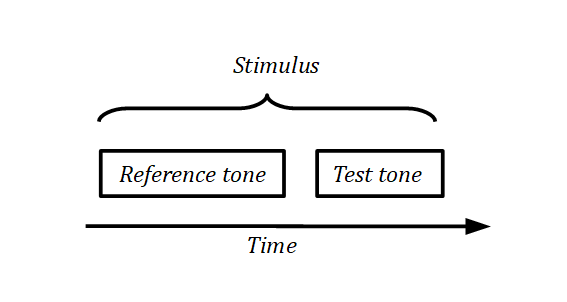
\includegraphics[scale = 0.5]{DiscriminationTask}
\caption{Schematic illustration of a stimulus in a discrimination task.}
\label{fig:discrtask}
\end{figure}

A stimulus in which the difference between reference and test tones is zero is called a \textit{noise} stimulus while one in which the difference is greater than zero is called a \textit{signal} stimulus; alternatively these can be called just noise and signal. 

\subsection{Signal Detection Theory}

Continuing the example of a  pitch discrimination task, during such experiment it is not rare to observe the participant sometimes give a negative and sometimes a positive response to the same stimulus on different presentations. The view that SDT takes is that the responses are not based directly on the physical signals, but rather some latent (unobserved) internal quantity, sometimes referred to as \textit{evidence} \citep{wickens2002} or \textit{judgments} \cite{stigler2003}, I will be using the term \textit{evidence} from here on. It is thought that the latent amount of evidence for e.g. the test tone being higher than the reference tone is subject to random variation, which in turn leads to variation in responses (\citet[p. 154]{kingdomprins2010}, \citet[p. 11]{wickens2002}). These random perturbations to the amount of evidence are commonly thought to arise primarily from sensory sources, but I will discuss this issue later in greater detail.

Some assumptions about the nature of the perturbations are usually made, for example that small perturbations are more common than large ones, and that the average amount of error is zero. A popular choice for modelling the distribution of the perturbations is the normal distribution with mean 0 and unknown variance. This is also the assumption that I will be making in this thesis. By making this assumption about the distribution of the perturbations, one can calculate the predicted response probabilities for different stimuli, and consequently make statistical inferences about the sensory processes of interest. Rest of the discussion will deal with the minutiae of these calculations. 

\subsubsection{Relationship between stimulus and $d'$}

Since the amount of evidence is assumed to be random, it can be represented as probability distributions as in Figure \ref{fig:SDT}. In the figure $S$ stands for physical signal level, for example the difference in frequencies between the reference and test tones. As was discussed in the previous section, normal distribution is used to model the distribution of evidence. 

If the subject is presented with a noise stimulus (one in which $S = 0$), the amount of evidence on any single trial is assumed to be a random sample from the zero-centred distribution in Figure \ref{fig:SDT}; in the context of the pitch discrimination task this would correspond with stimulus in which the test and reference pitches are identical. As $S$ is increased, the distribution from which the evidence is assumed to be sampled from shifts rightward, farther from zero, as is shown for $S = 2$ and $S = 4$.

\begin{figure}[!htb]
\begin{center}
\begin{knitrout}
\definecolor{shadecolor}{rgb}{0.969, 0.969, 0.969}\color{fgcolor}
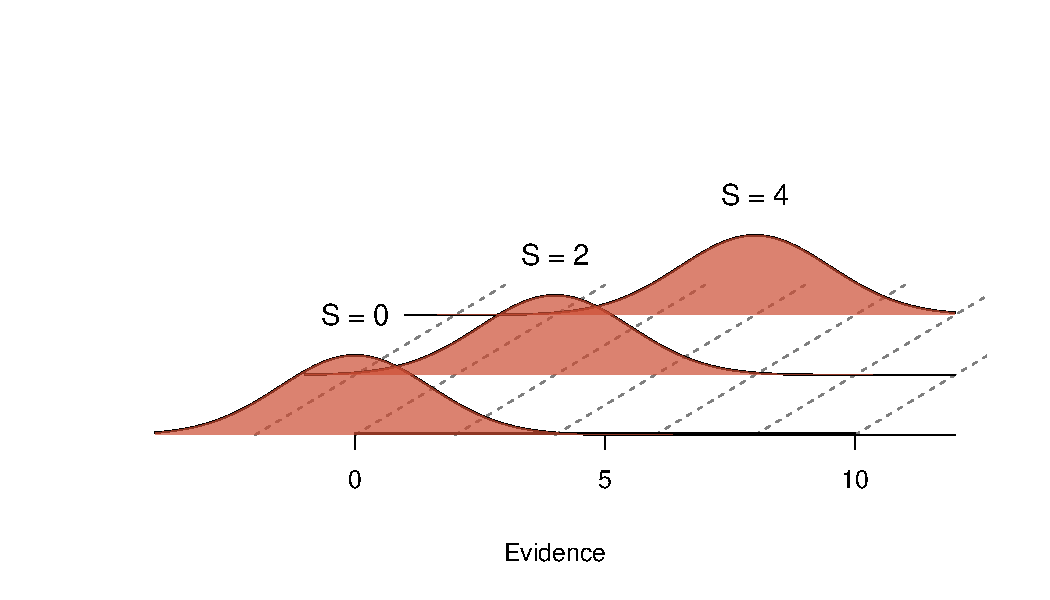
\includegraphics[width=\maxwidth]{figure/unnamed-chunk-2-1} 

\end{knitrout}
\end{center}
\caption{Evidence, according to SDT, is a random  variable. It can be assumed to be normally distributed, with monotonically increasing $\mu$ as a function of signal strength, $S$, and constant variance, $\sigma$.}
\label{fig:SDT}
\end{figure}

Signal level divided by the standard deviation of evidence is called $d'$, usually interpreted as \textit{discriminability} \citep[Chapter 6]{kingdomprins2010} or \textit{signal-to-noise ratio} \citep{kontsevichtyler1999}. Standardized in this way, the standard deviation of evidence distribution is always one, and the mean is $d'$, which is convenient. This is why usually the relationship between signal strength and $d'$ is modelled. 

The relationship between $d'$ and $S$ is not necessarily linear. Theoretically this kind of non-linearity could  arise e.g. from changes in the variance of the evidence distribution. However, the non-linearity is often interpreted as being the result of non-linearity in signal transduction, i.e. the change of physical signal into internal.\footnote{Familiar example of non-linear transduction is how pitch is experienced in large scale: in order to move one octave up on the psychological scale of pitch, one has to move increasingly fast on the physical frequency, see \citet[Chapter 5]{zwickerfastl}.}

The functional relationship between physical signal strength and $d'$ has been quantified in many different ways in the psychophysical literature (for a selection, see \citet[Appendix A]{lesmes2015}). The functional form used here is based on the widely used \textit{power law} model of signal transduction (see e.g. \citet{kontsevichtyler1999, dai2011, lesmes2015}):

\begin{equation}
d' = (\frac{S}{\sigma})^\beta
\label{eq:dprimefunc}
\end{equation}

Here $S$ is again the physical signal strength, $\sigma$ corresponds to the standard deviation of evidence and $\beta$ models non-linearity between signal level and signal-to-noise ratio. Note that often the letter $\alpha$ is used for the standard deviation of evidence (e.g. in \cite{dai2011, kontsevichtyler1999, kingdomprins2010}), but since this parameter is directly related to the standard deviation of the evidence distribution, I feel $\sigma$ is more appropriate. 

The effects of changing these parameters are shown in Figure \ref{fig:dprimefunc}. The smaller $\sigma$ is, the faster $d'$ increases. $\beta$ parameter affects the linearity of the function: when $\beta < 1$ the function increases faster than the linear case before the point at which $d' = 1$ and slower after that; the opposite happens when $\beta > 1$. 

\begin{figure}[!htb]
\begin{center}
\begin{knitrout}
\definecolor{shadecolor}{rgb}{0.969, 0.969, 0.969}\color{fgcolor}
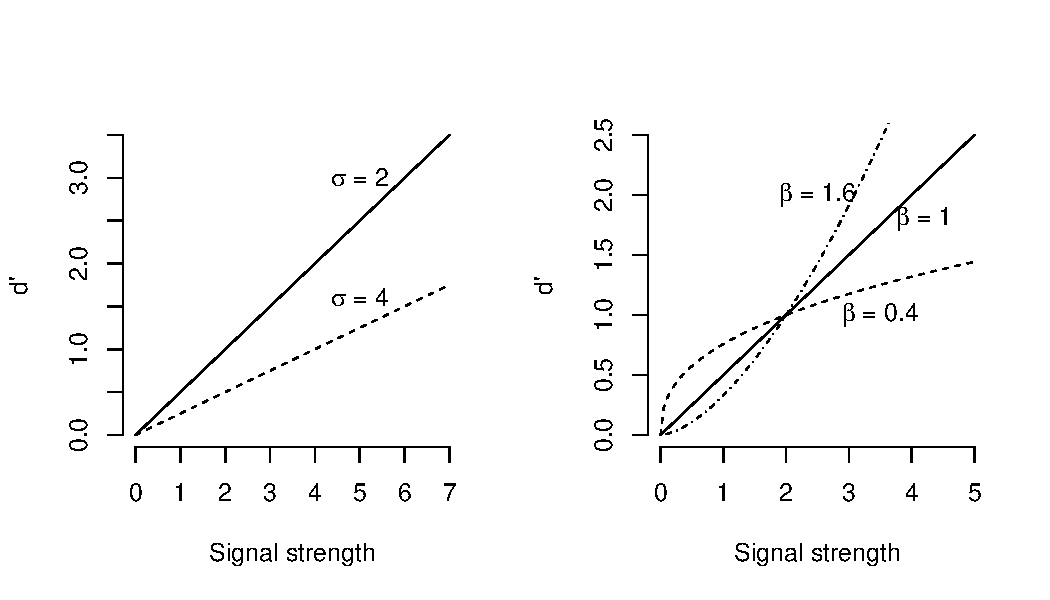
\includegraphics[width=\maxwidth]{figure/unnamed-chunk-3-1} 

\end{knitrout}
\end{center}
\caption{ The effect of $\sigma$ and $\beta$ parameters on the $d'$ function. Left panel shows the effect of changing $\sigma$ parameter while keeping $\beta$ constant ($\beta = 1$) and the right panel shows the effect of changing $\beta$ parameter while keeping $\sigma$ constant ($\sigma = 2$).}
\label{fig:dprimefunc}
\end{figure}

\subsubsection{Modelling responses: relationship between $d'$ and response}

The preceding discussion about relating $S$-values to $d'$-values is just one half of SDT, there has to be a way of relating the $d'$-values to responses, $R$. Usually categorical decisions are required from the participant, and the specific response categories depend on what kind of task they are performing. I will be considering a Yes/No and a 2-interval 2-alternative forced choice (2I-2AFC) tasks. These are shown schematically in Figure \ref{fig:YesNoAfc}.

\begin{figure}[!htb]
\centering
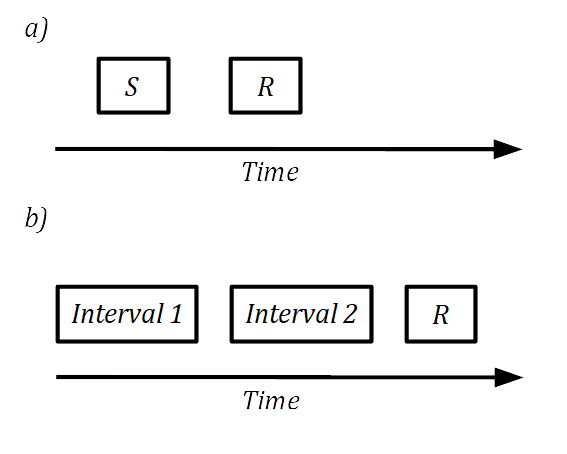
\includegraphics[scale = 0.5]{YesNoAfc}
\caption{Schematic representations of the Yes/No (panel a) and 2-interval forced choice (panel b) tasks. \textit{S = } signal, \textit{R =} response.}
\label{fig:YesNoAfc}
\end{figure}

In the Yes/No task (panel \textit{a} of Figure \ref{fig:YesNoAfc}) the participant's task is to indicate if they detected the signal. The name of the task is quite literal as the participants provide \textit{Yes} and \textit{No} answers. As shown in the figure, the participant is first presented with the stimulus after which they are expected to give their answer.

In contrast to this, in the 2I-2AFC task the participant is presented with two \textit{observation intervals}, interval referring here to a temporal interval as can be seen from panel \textit{b} of Figure \ref{fig:YesNoAfc}. During each interval the participant is presented with a stimulus, one containing only noise and the other containing the signal. The participant's task is then to indicate which interval they thought contained the signal. Again, the name is quite literal: the participant is presented with two \textit{intervals} and they have to choose their response among two \textit{alternatives}.

\paragraph{Responses in the Yes/No task}

Decisional processing in the Yes/No task is modelled by assuming that the participant has an internal criterion for the evidence: when evidence is below this criterion the participant will respond negatively and when evidence exceeds the criterion they will respond  positively.

When the participant is presented with a signal stimulus, positive responses are called \textit{hits}; when they  are presented with a noise stimulus, positive responses are called \textit{false alarms}. \citep{wickens2002, kingdomprins2010}. 

Criterion is represented by the red dashed vertical lines in Figure \ref{fig:yesno}. As signal level increases, and as a consequence $d'$, the evidence distribution shifts to the right. Since the criterion is fixed, larger portion of the evidence distribution falls to the right of the criterion, indicating higher probability of a positive response.

\begin{figure}[!htb]
\centering
\begin{knitrout}
\definecolor{shadecolor}{rgb}{0.969, 0.969, 0.969}\color{fgcolor}
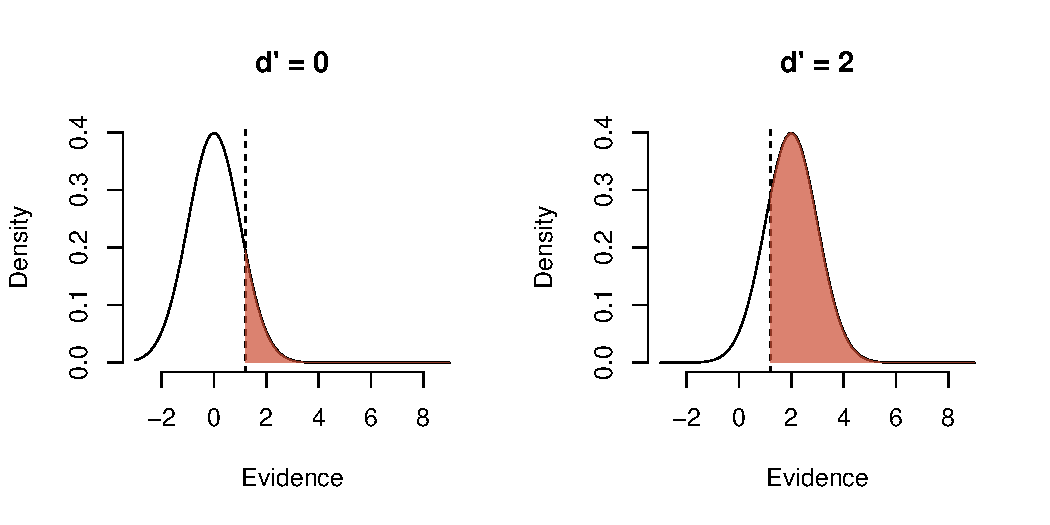
\includegraphics[width=\maxwidth]{figure/unnamed-chunk-4-1} 

\end{knitrout}
\caption{Binary decisions in the YesNo-paradigm. The distribution of evidence is divided into response regions.}
\label{fig:yesno}
\end{figure}

The probability of evidence exceeding the decisional criterion on any trial can be found by finding the area (shaded part in Figure \ref{fig:yesno}) under the normal distribution upwards from the criterion (see \citet{wickens2002, kingdomprins2010}):

\begin{equation}
\label{eq:SDTintegral}
P(R = 1) = \int_{c}^{\infty} N(d', 1)
\end{equation}

where $N$ is the normal distribution function with parameters $\mu$ (mean) and $\sigma$ (standard deviation), $d'$ is the signal-to-noise ratio as calculated in Equation \ref{eq:dprimefunc} and $c$, the lower bound of the integral, is the decisional criterion. 

The integral in this equation is usually written in terms of the cumulative standard normal distribution function, $\phi(u) = \int_{-\infty}^{u} N(0, 1)$. The resulting function, denoted with the Greek letter $\psi$, is called the \textit{psychometric function}. \cite[Chapter 4]{kingdomprins2010}

Usually only the positive response is considered, since the probability of a negative response is simply the complement of it, but it is more principled to show the probabilities for both the positive and negative responses:

\begin{align*}
\begin{split}
\psi(S; \theta)_{\text{Yes}} &= \phi(-c + d') \\
\psi(S; \theta)_{\text{No}} &=  1 - \phi(-c + d')
\end{split}
\end{align*}

Here $\theta$ is a vector containing the parameters of the psychometric function ($\sigma$, $c$ and $\beta$), and $S$ is the physical signal level. Given vectors of observed signals and responses ($S$ and $R$), one can find the best fitting values for the parameters, which then would taken as the Signal Detection Theoretical interpretation of the observer's performance. In this interpretation the performance is divided into sensory (parameters $\sigma$ and $\beta$) and decisional (parameter $c$) factors.

Since sensory and decisional processes are separate in the model, keeping the parameters that model sensory processing constant while varying the criterion will result in different predicted proportions of \textit{Yes} and \textit{No} responses and as a consequence hits and false alarms. That is to say that the perceptual processing capabilities can be exactly the same for two participants, but the observed amounts of hits and false alarms can be different, if one participant has different criterion. This is demonstrated in the left panel of Figure \ref{fig:critchange}: in the figure, parameters relating to sensory factors are kept constant while the criterion is varied. The psychometric function drawn with a solid line represents response probabilities for an observer with more lax criterion in relation to the dashed function.

It is also important to notice that hits and false alarms are coupled. If the participant wants to avoid false alarms, they will have to adopt a stricter criterion for the evidence, and  as a consequence they  will inevitably also make less hits. This is because the aim of SDT is to model situation in which there is a non-zero probability of confusing signal with noise. 

The coupling between hits and false alarms is demonstrated in the form the a \textit{receiver operating characteristic} (ROC) curve \cite[161]{kingdomprins2010} in the right panel of Figure \ref{fig:critchange}. The lines are drawn from two $d'$ values, dashed line representing a stronger signal relative to the solid line. When the participant adopts stricter criterion, they move left on the ROC curves: indicating not only higher proportion of hits but also false alarms. Conversely stricter criterion leads to less false alarms but also less hits.

The result is that if the participant aims to avoid false alarms altogether, they will have to adopt a criterion that, theoretically, would also result in zero hits; the criterion has to be relaxed a bit in order for the participant to perform in the task in any meaningful way, resulting in some false alarms and hits, as just discussed. Generally, the participant is free to "set their own criterion", however it is possible to calculate the optimal value of the decisional criterion. 

\begin{figure}[!htb]
\begin{center}
\begin{knitrout}
\definecolor{shadecolor}{rgb}{0.969, 0.969, 0.969}\color{fgcolor}
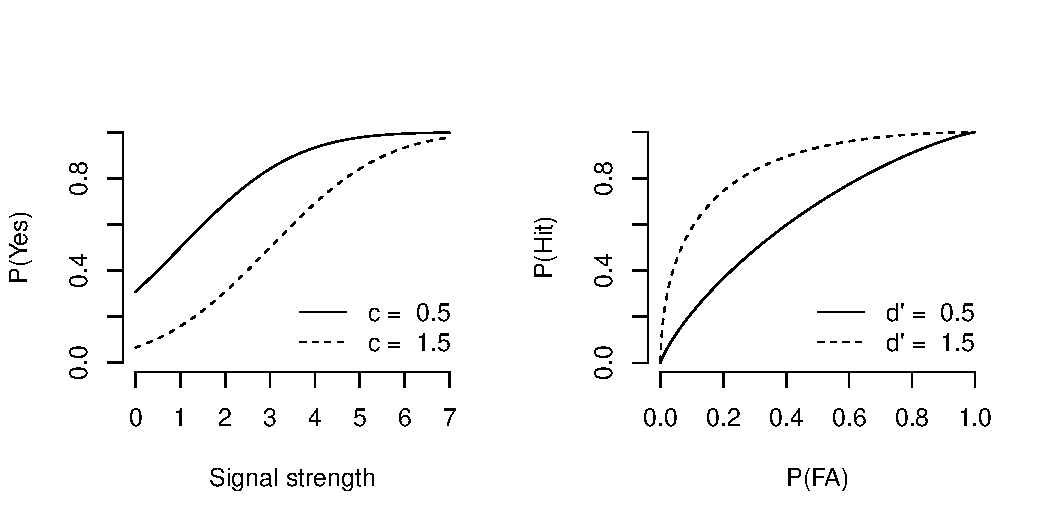
\includegraphics[width=\maxwidth]{figure/unnamed-chunk-5-1} 

\end{knitrout}
\end{center}
\caption{ Decisional processing in Signal Detection Theory. Left panel: The effect of differing criteria on the predicted amounts of false alarms and hits while the parameters describing the sensory processing are kept constant. \textit{Higher} criterion value implies stricter criterion--that the participant is less willing to respond \textit{yes}--while a \textit{lower} value implies more lax criterion. Right panel: Receiver operating characteristic (ROC) curve for two fixed $d'$-values, showing that the proportions of hits and false alarms are coupled.}
\label{fig:critchange}
\end{figure}

\paragraph{Responses in the 2I-2AFC task}

Since the participant is presented with two stimuli in the 2I-2AFC task, theoretically the participant is comparing two random numbers, one representing strength  of evidence in the first interval and the other representing strength of evidence in the second interval. From which ever interval the larger of these two was from gets picked as the \textit{signal} interval by the participant.

As a consequence the signal-to-noise ratio is decreased compared to the Yes/No task. Intuitively this can be understood by noticing that if one compares two things, both of which contain uncertainty, the individual uncertainties add up. Mathematically speaking, the participant can be thought of basing their decision on decision variable (here $dv$) that is the difference of the two random variables:

\begin{equation}
dv = [N(d', 1) - N(0, 1)] I
\end{equation}

Here $I$ is an indicator variable which  is $-1$ when the signal is in the first interval and $1$ when the signal is in the second interval. Consequently the decision rule is to respond \textit{Interval 1} when the decision variable $dv$ is negative and \textit{Interval 2} when it's positive. 

It is usually more practical, however, to think about the responses in terms of hits and false alarms, similar to the Yes/No task. This makes it possible to drop the the indicator variable from the equation, since we are only interested in the difference between the signal and noise distributions. This basic structure of the 2AFC model is demonstrated in Figure \ref{fig:2AFC}. 

\begin{figure}[!htb]
\centering
\begin{knitrout}
\definecolor{shadecolor}{rgb}{0.969, 0.969, 0.969}\color{fgcolor}
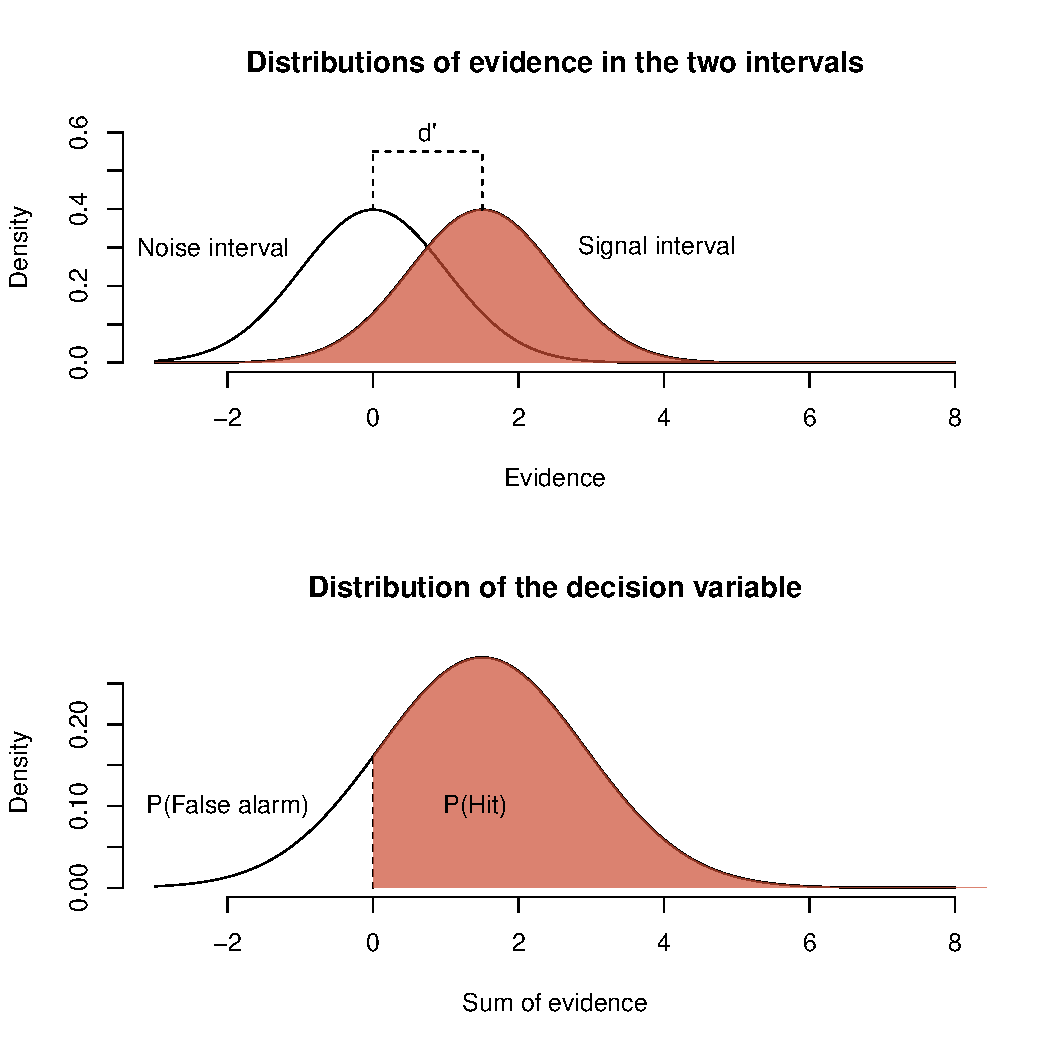
\includegraphics[width=\maxwidth]{figure/unnamed-chunk-6-1} 

\end{knitrout}
\caption{How responses are generated in the forced choice task. In the upper panel, the shaded distribution shows distribution of evidence from the signal interval while the non-shaded distribution shows evidence from the noise interval. The lower panel shows the distribution of the decision variable. }
\label{fig:2AFC}
\end{figure}

In the upper panel the zero-centred distribution represents evidence from the noise-only interval while the distribution centred on 1.5 represents evidence from the signal interval. Irregardless of whether the signal is in the first or second interval, the signal interval will be shifted $d'$ amount. Since the probability of making the correct decision is the proportion of the decision variable distribution that exceeds 0, shifting the signal distribution to the right will increase this probability--as one would expect.

What is important to note is that the decision variable is the difference of two normally distributed random variables, both with standard  deviation of one, since they represent the standardized quantity $d'$. It follows from the additivity of variances, and from the fact that standard deviation is the square root of variance, that the standard deviation of the decision variable is $\sqrt{1^2 + 1^2} = \sqrt{2}$. It follows then that the $d'$ values in the psychometric function have to be divided by this constant:

\begin{align*}
\begin{split}
\psi(S; \Theta)_{\text{Hit}} &= \phi(\frac{d'}{\sqrt{2}}) \\
\psi(S; \Theta)_{\text{False alarm}} &=  1 - \phi(\frac{d'}{\sqrt{2}})
\end{split}
\end{align*}

The term $c$ is dropped since it is assumed that, on average, the observer isn't biased towards either of the intervals. Some bias is probably not detrimental: any such bias would presumably be most noticeable when the signal level is low, and in these cases performance is already close to chance. 


%!Rnw root = ../Joni_Paakko_-_Thesis.Rnw

\subsection{General Recognition Theory}
\label{sec:grt_mdls}

So far I have covered the case in which the participant has to make a single decision, e.g. if the pitch of the stimulus changed. In the two-dimensional case the participant has to observe two things at once. For example did the pitch change \textit{and} did the timbre change. The question of primary interest is if there are any \textit{interactions} between the dimensions: does changing timbre also change response probabilities to pitch changes.

A widely used theoretical framework for generalizing SDT into multiple dimensions is the General Recognition Theory. As in SDT, also in GRT randomness in the responses is thought to arise from the evidence having a probabilistic nature \citep{ashby1986, ashby2015, kadlec1992}. 

In the two-dimensional case also the evidence distribution is two dimensional. Following the assumption made earlier that evidence is distributed normally, it is possible to represent evidence in two dimensions by a bivariate normal distribution. A bivariate normal distribution can be defined by two means, which correspond to its location on each dimension, and a correlation coefficient, which corresponds to the shape of the distribution. A bivariate normal distribution with positive correlation is shown graphically in Figure \ref{fig:2dimnorm}. Left panel shows a projection of the 3-dimensional shape of the bivariate density; right panel shows the same distribution from above, as a contour. Rest of the figures in this thesis will represent bivariate distributions as contours similar to the one in the right panel.

\begin{figure}
\centering
\begin{knitrout}
\definecolor{shadecolor}{rgb}{0.969, 0.969, 0.969}\color{fgcolor}
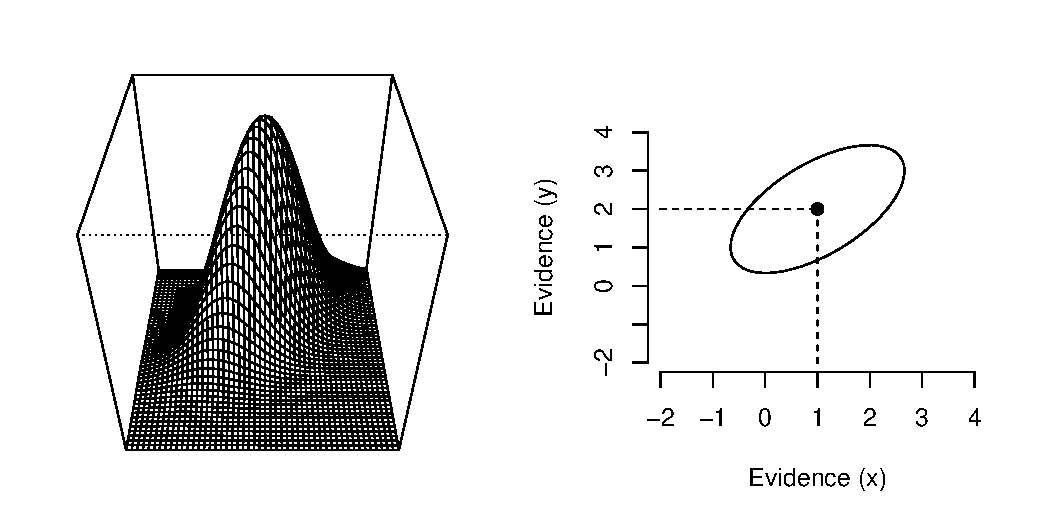
\includegraphics[width=\maxwidth]{figure/unnamed-chunk-7-1} 

\end{knitrout}
\caption{Two projections of a two-dimensional normal distribution with the parameters $\mu = [1.0, 2.0]$, $\rho = 0.6$.} 
\label{fig:2dimnorm}
\end{figure}

\subsubsection{Calculating $d'$ in two dimensions}

For two-dimensional stimuli, two $d'$ values have to be calculated, on for each dimension. Similar to SDT, the $d'$ values are the location of the evidence distribution, but now the location has to be determined in the two-dimensional space on the $x$ and $y$ axes separately: for example, how much evidence there is for a difference in pitch AND how much is there evidence for a difference in timbre. This implies that now there are two $d'$ functions, and consequently, two of each parameter: 

\begin{align}
\label{eq:twodimdprime}
\begin{split}
d'_x &= (\frac{S_x}{\sigma_x})^{\beta_x}\\
d'_y &= (\frac{S_y}{\sigma_y})^{\beta_y}
\end{split}
\end{align}

However, since the main motivation in GRT is to model interactions between the dimensions, this would be rather incomplete. I will first discuss how response probabilities are found in GRT, and then discuss the types of interference included in the models in this thesis.

\subsubsection{Modelling responses in two dimensions}
\label{sec:modelling_responses}

Whereas in SDT the participant is usually required to make a single decision on a single axis, in GRT the participant is required to make one decision per axis; in the two-dimensional case two decisions: did the signal level change on $x$ axis and did the signal level change on $y$ axis (a similar approach has been used also by \cite{wickens1992}). 

\paragraph{Yes/No task in two dimensions}

\begin{figure}
\begin{center}
\begin{knitrout}
\definecolor{shadecolor}{rgb}{0.969, 0.969, 0.969}\color{fgcolor}
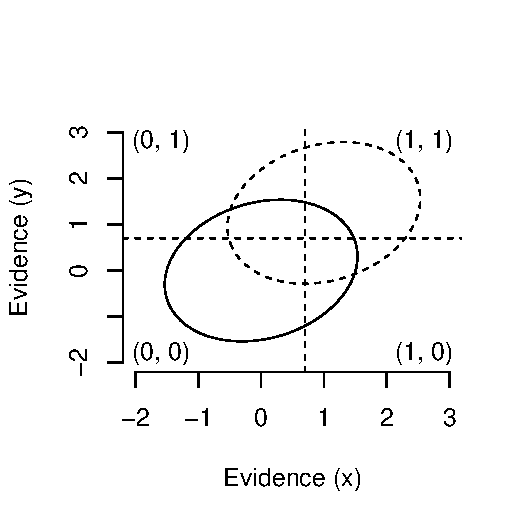
\includegraphics[width=\maxwidth]{figure/unnamed-chunk-8-1} 

\end{knitrout}
\end{center}
\caption{In two dimensions, the evidence distribution--when binary responses are required--is separated into four response regions.}
\label{fig:GRTsimple}
\end{figure}

Figure \ref{fig:GRTsimple} shows how the two-dimensional space is separated into response regions analogously to how it was shown from SDT Figure \ref{fig:SDT}. The distribution represented by the solid line has $d' = [0.00, 0.00]$ and the distribution represented by the dashed lines $d' = [1.00, 1.25]$. The dashed straight lines are the criteria: the vertical line is criterion for the dimension $x$ and the horizontal for dimension $y$. These criteria divide the two-dimensional space into four response regions. Most of the solid lined distribution falls into the region labelled $(0, 0)$ indicating high probability of a negative response on both dimensions. As the signal level on both dimensions is increased, as is done for the dashed line distribution, more of the distribution falls into the other regions, in this case the region $(1,1)$.  

Again, similar to unidimensional SDT, the response probabilities are found by integrating over the evidence distribution, split into response regions at the decisional boundaries as shown in Figure \ref{fig:GRTsimple}. For example the probability of observing a positive response on both dimensions is found by  integrating the two-dimensional normal distribution from the response criteria to positive infinity (region (1,1)). Whereas in the unidimensional case two psychometric functions were needed to model the two response categories, here four are needed, for each of the response possibilities:

\begin{align}
\begin{split}
\label{eq:probs}
\psi(\bm{S}; \theta)_{(\text{No}, \text{No})}  = \int_{-\infty}^{C_x} \int_{-\infty}^{C_y} N(\bm{\mu}, \bm{\Sigma})
\\
\psi(\bm{S}; \theta)_{(\text{Yes}, \text{No})}  = \int_{C_x}^{\infty} \int_{-\infty}^{C_y} N(\bm{\mu}, \bm{\Sigma})
\\
\psi(\bm{S}; \theta)_{(\text{No}, \text{Yes})}  = \int_{-\infty}^{C_x} \int_{C_y}^{\infty} N(\bm{\mu}, \bm{\Sigma})
\\
\psi(\bm{S}; \theta)_{(\text{Yes}, \text{Yes})}  = \int_{C_x}^{\infty} \int_{C_y}^{\infty} N(\bm{\mu}, \bm{\Sigma})
\end{split}
\end{align}

Here $\bm{S}$ is a vector containing the physical signal levels on the individual dimensions, $\bm{\mu}$ corresponds to the vector of $d'$-values. $\bm{\Sigma}$ is the correlation matrix, in which correlated evidence is modelled by treating the correlation coefficient as a free parameter:

$$
\begin{bmatrix}
1 & \rho \\
\rho & 1
\end{bmatrix}
$$

Similar to SDT, the psychometric functions are most practically thought about in terms of the (bivariate) standard normal cumulative distribution function, $\phi_2(u_x, u_y, \rho) = \int_{-\infty}^{u_x} \int_{-\infty}^{u_y} N([0,0], \bm{\Sigma})$, in which $\bm{\Sigma}$ is defined as before. The upper integration limits can be found by calculating:

\begin{align*}
\begin{split}
u_x &= -c_x + d'_x \\
u_y &= -c_y + d'_y
\end{split}
\end{align*}

Then, if responses are coded with $\text{No} = -1$ and $ \text{Yes} = 1$, inputs for the $\phi_2$ function are:

\begin{align*}
\begin{split}
\psi_2(\bm{S}; \theta)_{\text{(-1, -1)}} &= \phi_2(-1 u_x, -1 u_y, \rho [-1 * -1]) \\
\psi_2(\bm{S}; \theta)_{\text{(1, -1)}}  &= \phi_2(\phantom{-}1 u_x, -1 u_y, \rho [\phantom{-}1 * -1]) \\
\psi_2(\bm{S}; \theta)_{\text{(-1, 1)}}  &= \phi_2(-1 u_x, \phantom{-}1 u_y, \rho [-1 * \phantom{-}1]) \\
\psi_2(\bm{S}; \theta)_{\text{(1, 1)}}   &= \phi_2(\phantom{-}1 u_x, \phantom{-}1 u_y, \rho [\phantom{-}1 * \phantom{-}1]) 
\end{split}
\end{align*}

This process can be defined generally with the equation:

\begin{equation}
\psi_2(\bm{S}; \theta)_{\bm{R}} = \phi_2([-c_x + d'_x]r_x, [-c_y + d'_y] r_y, \rho [r_x r_y])
\label{eq:generalPfun}
\end{equation}

in which the $\bm{R} = [r_x r_y]$. All of the Stan \citep{stan2019} programs in the appendices assume that responses are coded in this way.

\paragraph{2I-4AFC}

In the SDT section I discussed the 2I-2AFC task. Here I expand it to the 2I-4AFC task. There are still two temporal intervals, as was shown in the schematic in Figure \ref{fig:YesNoAfc}, but now the participant has four response alternatives, since either signal could be in either interval: for example that pitch changed in the first interval and timbre in the second. The same dimension never changes in both intervals, that is, if there's a pitch change in the first interval, there never is a pitch change in the second interval.

Similar to Figure \ref{fig:2AFC}, Figure \ref{fig:2I4AFC} shows the distributions of evidence from the two intervals. Note that each of the signals could be in either of the intervals, so there are four possible arrangements for the signals, but similar to the case in 2I-2AFC it is not important in which intervals the signals are concretely, what is important is the difference between the signal and noise distributions. 

It is assumed in Figure \ref{fig:2I4AFC} that $\kappa_{x}^{\mu}$ parameter is non-zero, which means that signal on $y$-dimension is able to increase the $d'$-value on the $x$-dimension--the interaction parameters, which $\kappa_{mu x}$ is one of, will be defined more comprehensively in the next section. This can be seen from the fact that in the left panel the mean of the noise distribution on the $x$-axis is slightly greater than zero. If such interaction was absent, the mean of the noise distribution would be zero on both dimensions, there would be on average no evidence for change in either dimension. The interaction shrinks the difference between the signal and noise distributions on that dimension.

As before, the participant is thought to base their decision on a decision variable that represents the difference of evidence in the intervals. As a consequence the $d'$ values on both dimensions have to be divided by $\sqrt{2}$ (cf. section on 2I-2AFC). The distribution of the decisional variable can be seen in the right panel of Figure \ref{fig:2I4AFC}. The thick black lines mark boundaries between \textit{hits} and \textit{false alarms}. The participant, in this particular scenario, is very likely to score a \textit{hit} on the $y$-axis, but on $x$-axis they are almost as likely to pick the wrong interval as the correct; the most likely response pairs being (FA, Hit) and (Hit, Hit).

\begin{figure}
\centering
\begin{knitrout}
\definecolor{shadecolor}{rgb}{0.969, 0.969, 0.969}\color{fgcolor}
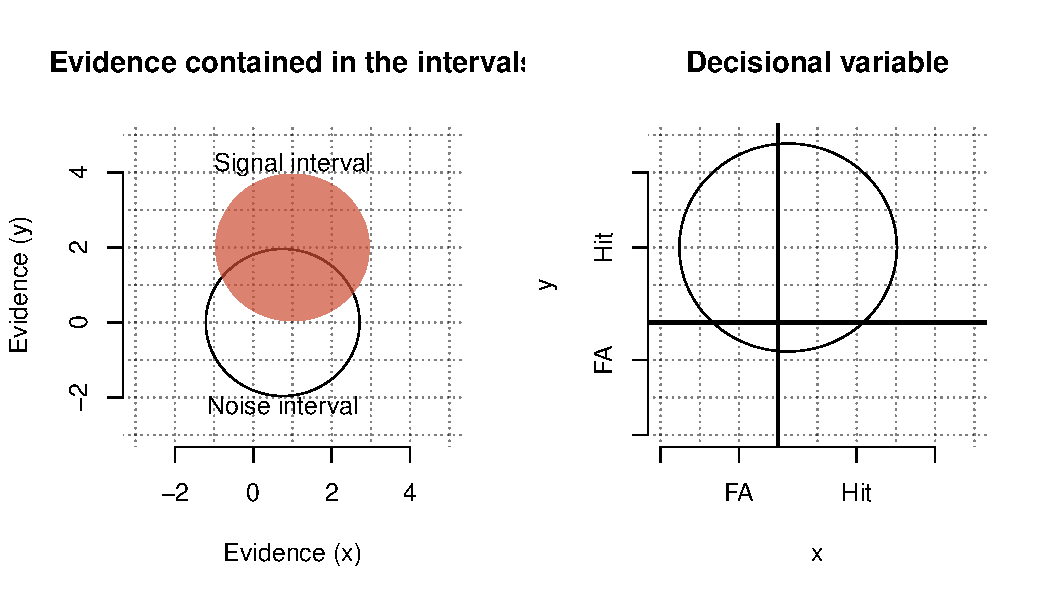
\includegraphics[width=\maxwidth]{figure/unnamed-chunk-9-1} 

\end{knitrout}
\caption{In the 21-4AFC task, the participant is assumed to base their responses on the difference in the evidence from signal and noise distributions (left panel). Variance of the distribution of differences is th sum of the variances of the individual distributions (right panel).}
\label{fig:2I4AFC}
\end{figure}

As in the Yes/No task, responses can be coded with -1 and 1. Here, \textit{false alarms} are coded with -1 and \textit{hits} with 1.  The general expression for the psychometric function is then

\begin{equation}
\psi_2(\bm{S}; \theta)_{\bm{R}} = \phi_2(\frac{d'_x}{\sqrt{2}}r_x, \frac{d'_y}{\sqrt{2}} r_y, \rho [r_x r_y])
\label{eq:generalPfun2}
\end{equation}

\paragraph{Comparison of the Yes/No and 2I-4AFC tasks}

The main difference between the Yes/No and 2I-4AFC tasks is what the participant's decision is directly related to. In the Yes/No task the decision is about the \textit{appearance} of the stimulus. As was already discussed, this means that the performance of the observer cannot be decoupled from their decisional criterion. This adds one more parameter to be estimated from the data. 

In the 2I-4AFC task the decision about the \textit{interval}. This means that it is not necessary for the participant to adopt a criterion relating the strength of evidence to a response. Also, since the participants are choosing an interval, which is by its nature more neutral decision, it is usually thought that this kind of task is less susceptible to bias \citep[Chapter 6]{kingdomprins2010}.

Since on each trial two stimuli have to be presented in the 2I-4AFC task, it is somewhat slower to administer. However, if the observer knows, in the Yes/No task, that some non-zero signal is present on each trial, nothing prevents them from answering \textit{yes} on each trial--they will always be correct, and seemingly able to detect the faintest of signals. To counter this, some amount of \textit{catch} trials are usually included. These are trials during which the signal level is zero. During these trials no information about the sensory processing--the parameters $\sigma$ and $\beta$--is accumulated. So even though individual trials are faster to complete, there has to be more of them. 

The issue of catch trials is exacerbated in the multidimensional case. This is because in the one-dimensional the issue is simple solved by including some noise stimuli as catch trials in the experimental run, resulting in two kinds of stimuli being presented: noise and signal stimuli. In the two-dimensional case there has to be three kinds of catch trials: noise only stimulus on either of the dimensions or both. Otherwise if the participant became aware of e.g. that the adaptive procedure only rarely selects a stimulus in which there's a noise stimulus on one dimension--i.e. [0,S] or [S,0] --, they might become biased towards choosing the responses [No, No] and [Yes,Yes]. The linear decision bounds used in this work are not able to model this kind of response bias; an issue which will be discussed later. 

Then, on theoretical grounds, the only difference to be expected is the omission of the criterion parameters from the 2I-4AFC model--reduction in sensitivity is taken into account by incorporating the term $\sqrt{2}$. 

\subsubsection{Interactions between the dimensions}

As already discussed GRT aims to model \textit{interactions} between the dimensions. When the one dimension has an effect on the other, this is called \textit{interference}. There are three kinds of interactions considered in this thesis. Two of these interactions are defined as \textit{couplings} between the psychometric functions, and the third interaction is the correlation of the evidence distribution, but since including correlation coefficient was already conclusively discussed in the preceding section, I will only discuss the couplings here.

Two kinds of couplings are modelled. These are demonstrated graphically  in Figure \ref{fig:grt_couplings}. Panels in the left column demonstrate coupling between means while panel on the right side demonstrate coupling between standard deviations. Top row shows effects of the interactions on the evidence distributions while the bottom row shows the effect on the psychometric function on one dimension.\footnote{mathematically the union of the psychometric functions $\psi{\bm{S}}_{(\text{Yes}, \text{Yes})}$ and $\psi{\bm{S}}_{(\text{Yes}, \text{No})}$.} In all panels dashed lines show the situation in the absence of interaction while the solid lines are drawn in the presence of interaction. 

\begin{figure}
\begin{center}
\begin{knitrout}
\definecolor{shadecolor}{rgb}{0.969, 0.969, 0.969}\color{fgcolor}
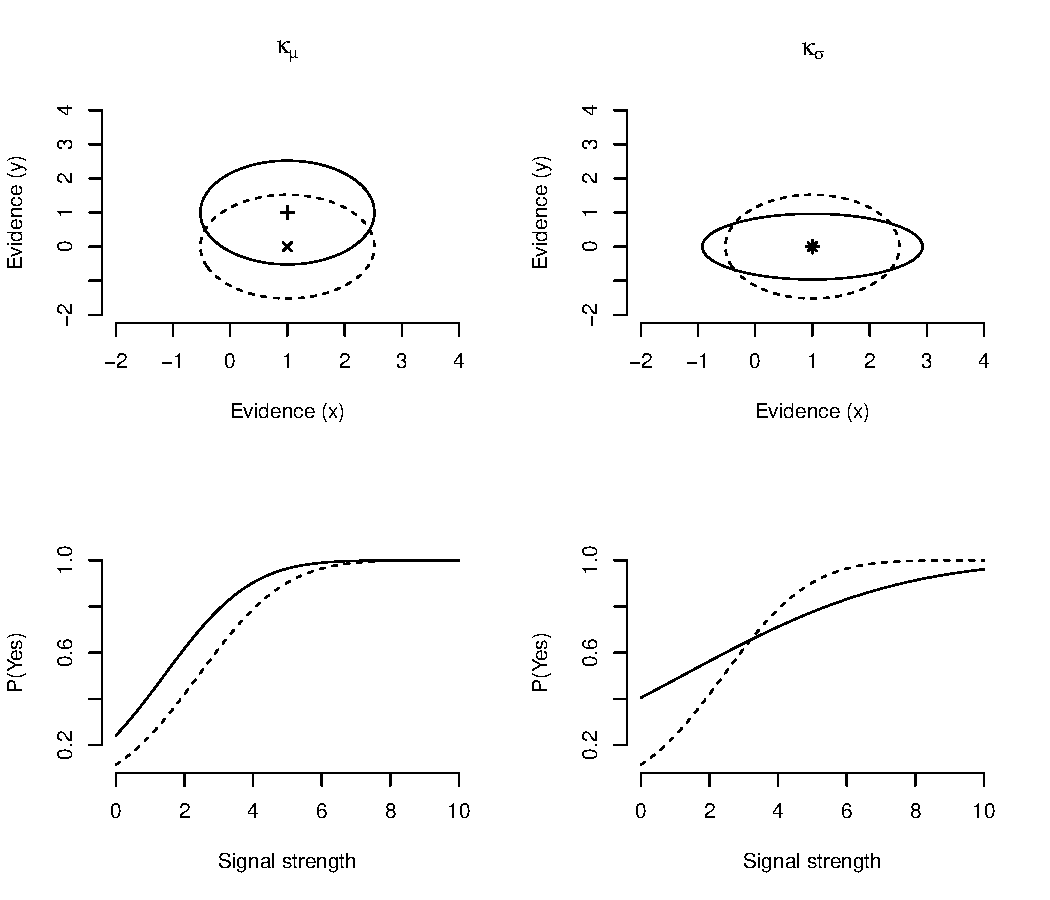
\includegraphics[width=\maxwidth]{figure/unnamed-chunk-10-1} 

\end{knitrout}
\end{center}
\caption{The two kinds of couplings in the model. The contours in the top row depict bivariate normal distributions. Dashed lines indicate the shape and location of the distribution in the absence of interaction; the solid lines depict them in the case that interaction is present. Curves in the lower row are psychometric functions for a single dimension.}
\label{fig:grt_couplings}
\end{figure}

\paragraph{Coupled means, $\kappa_{\mu}$}

Coupling between the means of the distributions is modelled by letting the other dimension influence the $d'$ values: 

\begin{align}
\label{eq:kappa_mu}
\begin{split}
d'_x &= (\frac{S_x}{\sigma_x})^{\beta_x} + \kappa_x^{\mu} S_y \\
d'_y &= (\frac{S_y}{\sigma_y})^{\beta_y} + \kappa_y^{\mu} S_x
\end{split}
\end{align}

As can be seen from the lower left panel of Figure \ref{fig:grt_couplings} this kind of interactions shifts the psychometric on the affected dimension. Here, the presence of interference has increased the $d'$ values and consequently probabilities for positive responses all along the range of the function.

\paragraph{Coupled standard deviations, $\kappa_{\sigma}$}

Another possibility is that the standard deviations are coupled. This kind of situation can arise if for example the other dimension is length: shorter signals contain less information, thus making frequency judgments noisier (see \citet[p.274]{houtsma1995}, also worse accuracy with shorter signal times has been reported by e.g. \cite{townsend1988} implying more noise).

Similar to $\kappa_{\mu}$, terms are included for letting the other dimension influence the $\sigma$ parameter. However, since the $\sigma$ parameters are constrained to positive real numbers (standard deviation can't be negative), this interaction is defined on the logarithmic scale (for a similar approach in probit modelling, which is closely related to SDT as will be discussed shortly, see \citet{freeman2018}):

\begin{align}
\label{eq:varshift}
\begin{split}
\sigma_x &= exp(log\sigma_x + \kappa_x^{\sigma} S_y) \\
\sigma_y &= exp(log\sigma_y + \kappa_y^{\sigma} S_x)
\end{split}
\end{align}

When the model parameters relating to response boundaries or criteria--as is the case in here for the \textit{Yes/No} model--they also have to be divided by the standard deviation. This is intuitively clear from the observation that as the spread of the evidence distribution becomes larger, the parts of the evidence distribution falling into the response regions become increasingly equal. In other words response probabilities get closer to 0.25, and a larger denominator for the term $c$ will achieve just this:

\begin{equation}
\psi_2(\bm{S}; \theta)_{\bm{R}} = \phi_2([-\frac{c_x}{\sigma_x} + d'_x]r_x, [-\frac{c_y}{\sigma_y} + d'_y] r_y, \rho [r_x r_y])
\label{eq:generalPfun_varshift}
\end{equation}  

This means that the definition of criterion is a bit different from that of when no coupling between standard deviations is present. In the model with constant variance, the criterion corresponds to the Z-score of the false alarm probability (see \citet[Chapter 6]{kingdomprins2010}): $\text{criterion} = \phi^{-1}(P(FA))$, in which $\phi^{-1}$ is the standard normal inverse cumulative distribution function; in the model with coupled standard deviations the whole first term corresponds to the Z-score of false alarm probability: $\frac{\text{criterion}}{\sigma} = \phi^{-1}(P(FA))$. This means that in this model the criterion parameter is more accurately the geometric location of the decisional criterion in the decisional space, independent of the variance of the evidence distributions. However, since it is easier to interpret false alarm probabilities, prior in the models is placed on the term $\frac{\text{criterion}}{\sigma}$--what this means in practice will be discussed in the section on Bayesian statistics

From the lower right panel of Figure \ref{fig:grt_couplings} one can see that the effect is to draw the response probabilities towards 0.5 on a single dimension. Note that this is in agreement with what was said earlier about response probabilities being drawn towards 0.25: since the psychometric function in the figure is shown only for one dimension, it represents the probability of a positive response irregardless of the other dimension. 

\paragraph{Model with both kinds of couplings}

The most realistic case is one in which both kinds of couplings are included in the model. This is achieved easily by using Equation \ref{eq:kappa_mu} and calculating the $\sigma$ terms as in Equation \ref{eq:varshift}.

\paragraph{Note on terminology} 

The couplings, $\kappa_{\mu}$ and $\kappa_{\sigma}$, are sometimes called \textit{between stimuli/distributions interference} \citep{silbert2009} and the situation in which they are absent can be referred to as \textit{sensory independence} \citep{ashby2015}. Correlation can be called \textit{within stimulus/distribution interference} \citep{silbert2009} and the absence of correlation as \textit{perceptual independence} \citep{ashby2015}. In addition, $\kappa_{\mu}$ can be called \textit{mean-shift integrality} and $\kappa_{\sigma}$ \textit{variance-shift integrality} \citep{ashby1994}.

\subsection{Lapsing behaviour}
\label{sec:lapses_general}

It is possible that during a psychophysical task, people sometimes \textit{lapse}. That is, for some reason the response they give doesn't reflect the cognitive process of interest. This might be due to e.g. lapse in attention, a coding error in the program, or a slip of a finger. In the classic GRT models, lapsing behaviour has not been taken into account, even though in the unidimensional case lapses have been shown to be able to exert considerable bias on the parameter estimates of the psychometric function \citep{wichmannhill2001}. 

Estimating lapsing rate from data can be problematic (\cite{wichmannhill2001, treutwein1999}), and this problem can be worse for adaptive procedures \citep{prins2012}. Since the values of the psychometric function that are closer to zero are affected both the lapses and the decision criterion (in the Yes/No task), most of the information gained about lapsing behaviour comes from lapses happening at high intensities. What makes matters worse is that the lapsing response doesn't necessarily differ from what the participant would've answered otherwise, so the distinction between lapses and genuine response is ambiguous (for further discussion on these problems, see \cite{prins2012}). For these reasons I fixed the values of $\lambda$ and $\gamma$ during the adaptive estimation phase. However, during the analysis of the psychophysical data I estimated the parameter $\lambda$ from the data, a decision, which will be discussed in more detail in the analysis section.

I model lapsing behaviour by using a (hierarchical) mixture model (see \citet{zeigenfuse2010}), which will be discussed in Section \ref{sec:hierarchical_models} \textit{\nameref{sec:hierarchical_models}}.


%!Rnw root = ../Joni_Paakko_-_Thesis.Rnw

\subsection{Critical discussion}
\label{sec:grt_criticism}

\subsubsection{Relationship to other models}

\paragraph{Classic GRT}

I will begin by discussing what I will call a \textit{classic} GRT model, and argue for the two main modifications implemented in this work: first abandoning the ubiquitous categorization task and second incorporating some functional for between the physical signal levels and the internal quantities. 

In the classic model the signals of interest are two-dimensional, the participant is required to hold one decisional criterion per dimension, and the method of constant stimuli (MOCS) is employed. Method of constant stimuli means that the levels of stimuli are fixed prior to the experiment. When two levels are used per dimensions, the experiment is called a 2x2 identification experiment.  A possible stimulus set is demonstrated in Table \ref{table:classicGRT}. I call this the classic model since it is the most widely--and in some cases the only--discussed type of model in GRT related literature (see e.g. \cite{ashby2015, ashby1986, cohen2003, kadlec1992, silbert2010, silbert2013}). 

\begin{table}[!htb]
 \centering
  \caption{An exemplar set of stimuli that could be used in a 2X2 identification experiment. The exact levels of e.g. high and low pitch are chosen a prior by the experimenter.}
  \vspace{0.5cm}
  \label{table:classicGRT}
   \begin{tabular}{rccc}
    \hline
     &       &         \multicolumn{2}{c}{Pitch} \\
                       \cline{3-4}
             &         & Low             & High   \\
     \hline
    \multirow{2}{*}{Timbre} 
            & Bright & \parbox[t]{5cm}{Low pitch + Bright timbre\\}& \parbox[t]{5cm}{High pitch + Bright timbre\\}\\
            & Dark    & \parbox[t]{5cm}{Low pitch + Dark timbre \\}  & \parbox[t]{5cm}{High pithc + Dark timbre \\ }\\
     \hline
    \end{tabular}
\end{table}

The logic in this kind of task differs from that of discrimination task. Instead of responding to differences in the stimuli, the participant's task is to categorize\footnote{Note that the term \textit{categorization} has it's own specific meaning distinct from identification in GRT literature (see \citet{ashby2015}), but here I'm using the term rather colloquially--and in any case, I believe the problems discussed here to apply both categorization and identification tasks.} the stimuli as if categorizing apples and oranges into their respective piles. The image of categorizing something into piles is surprisingly apt, since in the classic speeded classification experiments--which have been influential to the study of multidimensional perception, including GRT--\citep{garner1974} the participants would categorize visual stimuli printed on cards. 

Categorization is sensible in the case of clear differences, e.g. categorizing extremely different pitches such as 100 Hz and 5000 Hz. However, in the case of minute differences that are close to the detection threshold, it is more likely that the subject bases their decisions on perceived \textit{differences} between consecutive stimuli. One of the assumptions of the model is that single responses are statistically independent (see e.g. \citet[p. 218]{wickens1992}), but if indeed the responses are based on perceived differences between consecutive stimuli, this assumption is gravely violated.

Another difficulty is that the participant would have to hold accurate representations of the stimuli in their memory. Again this is simple when categorizing apples and oranges, but much more difficult in a psychophysical experiment in which the levels are to begin with selected in such a way that they are easily confusable. 

Of course all kinds of assumptions are always violated, since any statistical model is a simplification of the real and complex cognitive processes, but I feel it is better to use tasks that don't correspond with what can be realistically expected from the participant. It is for these reasons that I've opted to base the model presented here explicitly on discrimination instead of categorization or identification.

As per the second modification, the addition of functional relationships, in the classic GRT model each stimulus is represented by its own bivariate  normal distribution (see e.g. \cite{ashby2015}). For example, in the aforementioned 2X2 categorization task parameters for four bivariate normal distributions would be estimated. If more stimuli are used also more decision boundaries are needed in the categorization task: a separate set of decision boundaries between each category is required. 

This can lead to difficulties when trying to interpret the model. Consider for example the hypothetical case in Figure \ref{fig:classicGRT}: it is very difficult to come up with a simple summary of how the dimensions $x$ and $y$ are related. This is not only a problem for concise communication of results, but it is a theoretical problem: in my view modelling should strive towards more complete models, and staying agnostic about the functional forms of interactions does not advance this goal. 

\begin{figure}[!htb]
\centering
\begin{knitrout}
\definecolor{shadecolor}{rgb}{0.969, 0.969, 0.969}\color{fgcolor}
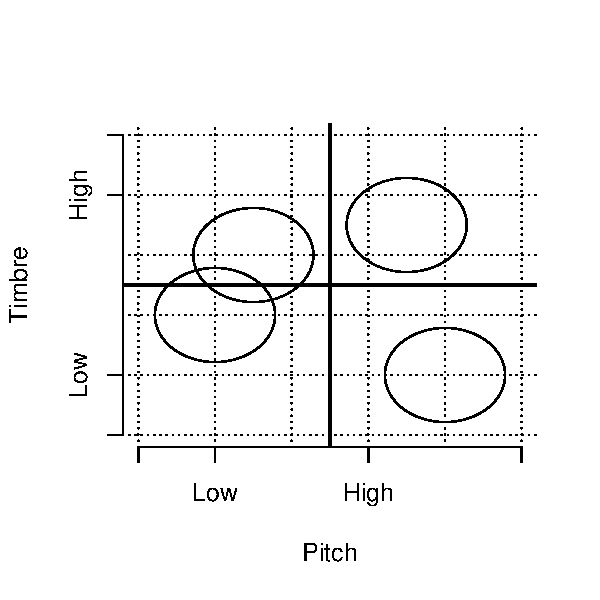
\includegraphics[width=\maxwidth]{figure/unnamed-chunk-11-1} 

\end{knitrout}
\caption{An example of a classic GRT model fitted to a 2X2 categorization data. Each of the stimuli are fitted with their own bivariate normal distribution.}
\label{fig:classicGRT}
\end{figure} 

Related difficulty is that it is hard to know, e.g. in the case depicted in Figure \ref{fig:classicGRT} which of the features of the data are purely coincidental and which of them accurately represent real dimensional interactions. Statistically speaking one could be \textit{overfitting}; a problem that is also recognized in the context of classic GRT models by \cite{soto2017}. Also, often the fit of the model is assessed by comparing the predicted response probabilities with the observed proportions (see for example \citet[Figure 4]{silbert2009}), but if a separate distribution is fitted to each stimulus, the model is overly flexible, and it is likely that \textit{any} data set would be matched very closely by the model. As such, this close match is not evidence for the veracity of the model; it is evidence for it's flexibility.

The current model rectifies these problems. Interactions are summarized by the $\kappa$ and $\rho$ coefficients, so it's easy to make inferences. Since the model is constrained by the explicit functional relationship between signal levels and $d'$, it's less prone to the type of overfitting described. 

\paragraph{Process model}

The interactions in the model can be conceptualized by hypothesizing a process structure to the model, as in \cite{ashby1989}, \cite{ashby2000} or \cite{cohen2003}. This is demonstrated in Figure \ref{fig:GRTprocess}. On each channel the physical signal, $S$, is transduced to the internal representation of the signal, $s$, after which it is judged against the decisional criterion, $c$, and the participant gives their response, $R$. The straight lines from a stage to the next--for example from $S_x$ to $s_y$ denote an influence to the average level of the variable while curved lines inside a stage--for example from $s_y$ and $s_x$--denote correlated noise. 

The effect of the signal level on the average level of the internal signal on the other channel is usually referred to as stage 1 interaction, the correlation of noise between the internal representations is referred to as stage 2 interaction, and the the dependence of the criteria on the internal level of the signal or correlation between their noise is referred to as stage 3 interaction. Stage 1 and 2 interactions are referred to as \textit{perceptual} interactions, and stage 3 interaction is referred to as \textit{cognitive} interaction. \citep{ashby1989, ashby2000, cohen2003}. 

\begin{figure}[!htb]
\centering
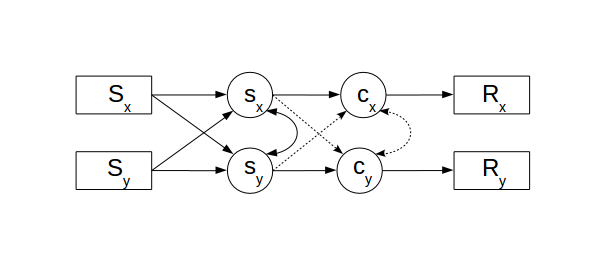
\includegraphics[scale = 0.8]{Process_model}
\caption{A process interpretation of the model. Variables inside rectangles are observed, whereas variables inside squares are latent. }
\label{fig:GRTprocess}
\end{figure}

In the current model, stage 1 interactions are modelled by the $\kappa$ terms while the stage 2 interaction is modelled by the correlation parameter $\rho$. Stage 3 interactions are not modelled, since, as the model currently stands, they are not identifiable. This issue will be discussed in greater detail later. 

\paragraph{Relationship to Generalized Linear Models}

Generalized Linear Models (GLM's) are widely implemented in statistical analysis (see e.g. \citet{kruschke2015, skrondahl2004}). The theoretical links to well-known models in statistics mean that the model should be easily generalizable to different situations, and that there exists a wide range of theoretical and empirical literature. 
 
\cite{decarlo1998} describes the unidimensional SDT model as a generalized linear model. In the case of normally distributed noise, a \textit{probit model}, which is how already Gustav Fechner--who is sometimes regarded as the founder of psychophysics--modelled categorical judgments in the 19th century (discussed in \citealt[Chapter 7]{stigler2003}). 

The models--with the caveat mentioned at the end of this section--used in this thesis can be thought of as a \textit{non-linear multinomial} probit model. Non-linear \citep[p. 379]{box2005} since the relationship between $S$ and $d'$ included the term $\beta$; multinomoal, since in a binary choice probit model the responses are assumed to follow the binomial distribution, but in the multidimensional model, since there are more than two choices, the responses are assumed to follow the multinomial distribution \cite[p. ERROR]{skrondahl2004}. 

As Generalized Linear Models in general, also the model here can in theory use any distribution as the model for the errors (the use of other than normal distributions in GRT has already been discussed in \citet{ashby1986}, but to my knowledge, other distributions besides normal have \textit{never} been used). The main limitation is mathematical and computational: how to effectively calculate the two-dimensional integrals needed for the response probabilities. There can also be other issues, e.g. for the  typical multinomial logistic model, no correlation is usually modelled \citep{skrondahl2004}, which can prove to be a too limiting assumption.

In the context of GLM's, the modelling of lapses is can be called \textit{robust regression} \citep[p. 635]{kruschke2015} since it relaxes the distributional assumptions somewhat, and isn't so prone to estimation errors due to outliers. However it should be noted that this requires the lapsing parameters to be fixed \citep[p. ERROR]{skrondahl2004}. This is not true for all of the models used in this thesis.

\subsubsection{Nonidentifiabilities and other limitations of the model}

\paragraph{What do the latent distributions really represent?}

The main assumption of SDT, and consequently GRT, is that the participant bases their decisions on noisy latent quantities. Therefore, it is important to discuss what those latent quantities actually represent.  

In SDT literature writers are generally careful to call the latent quantities evidence \citep{wickens2002, verde2006} or judgments (\citealp[p. 247]{stigler2003}). In GRT related literature, however, the latent quantities are thought to be more closely related perceptions. \cite{ashby2015} call them \textit{perceived values}; in \cite{ashby1986},  \cite{kadlec1992} and \cite{silbert2009} they are \textit{perceptual effects} and the space (in which the distributions are defined in) is defined as \textit{perceptual space}; \cite{soto2017} uses the term \textit{perceptual representation}.

As is clear from the preceding discussion on SDT and GRT, I've taken the more traditional way of calling the latent variables evidence, but even in this case one has to be careful in considering \textit{what} the evidence is about. Concretely the latent quantities are a sum of \textit{everything} that creates variability in responses: noise in encoding the signals, internal noise due to e.g. blood pressure or breathing, transient noises from sneezing or swallowing etc., lapses of attention, criterial changes, non-stationarity of threshold, effects of learning and so on. 

It is clear that for example in a pitch discrimination task many of the aforementioned factors don't necessarily directly effect the perceived amount of pitch difference, but can and will affect the judgments or amount of evidence in other ways, for example by masking the signal and limiting information that way.

Often there seems to be two strong implicit assumptions. First, that either the first factor would be significantly greater than any of the others, and second that any effect is sufficiently free from other influences. While these assumptions might not be that dangerous in SDT models, the problem is exacerbated in GRT: there is virtually no information about how the aforementioned factors influence e.g. inferences about interactions between the dimensions, a problem recognized already by \citet{silbert2009}. It is my impression, based on my own unpublished simulation studies, that the factors just mentioned can in some situations lead to significantly incorrect inferences. 

Validity of the process model described earlier relies heavily on these strong assumptions and our ability to differentiate between different sources of variation. It is my belief that in the current formulation, using straightforward perceptual experiments, one can not properly identify these, and indeed has to rely on strong prior assumptions. For this reason I would, at this point, see the process model more as a helpful conceptualization than anything else.

Conceptualization of the latent variables affects the way interactions are understood theoretically. Based on the preceding discussion I hope it is clear that it is different to say that e.g. timbre influences the distribution of \textit{evidence} about pitch than it is to say that timbre influences the distribution of \textit{perceptual effects} of pitch.

\paragraph{Criterial noise}

Criterial noise can be defined as random variation in the criteria around some central value, in the present context the central value would most naturally be thought of as the parameter $c$ in the model. If this variation is assumed to be Gaussian, it is not identifiable from other sources. This issue has been discussed in SDT literature already by \cite{wickelgren1968}\footnote{\cite{wickelgren1968} talks about \textit{unidimensional strength theory}, but the discussion is directly applicable to the present situation.}; in the context of GRT \citet{ashby2000} has discussed the role of criterial noise. In the context of SDT there have been proposals for identifying the magnitude of criterial noise using experimental manipulations (see e.g. \citealt{kellen2012, benjamin2009, cabrera2015}), but the application of these methodologies to GRT will not be considered further here. 

In practice, any criterial noise will be included in the $\sigma$ estimates, since, as already discussed, these represent to sum total of all variation. With regard to GRT the problem is if the criterial noise between the dimensions is correlated: this will be included in the $\rho$ estimates. Another possibility is that criterial changes--e.g. between sessions or during a long session--would also affect the $\kappa$ estimates. To my knowledge, no systematic exploration of this possibility exists; in my own non-systematic simulations I have noticed that indeed in some cases such criterial shifts can affect the the parameter estimates and lead to erroneous inferences. 

\paragraph{Non-orthogonality of decisional boundaries}

Another topic tying into the modelling of decisional processing is the (possible) non-orthogonality of the decisional boundaries. In the GRT literature non-orthogonal decisional boundaries are seen as failure of \textit{decisional separability} \citep{ashby2015}, since non-orthogonality implies that the decision is contingent on the level of the signal on the other dimension. 

In the present paper the focus is on orthogonal decisional boundaries. Non-orthogonal boundaries could be incorporated in the model, \cite{ennis2003} have shown a simple method for calculating the non-orthogonal integrals to evaluate the response probabilities. However, what could prove to be problematic is that the method, in my experience, is rather slow.  

Another problem is the identifiability of non-orthogonal decisional boundaries: \cite{soto2015} claim that their model makes decisional separability identifiable--contrary to the classic model \citep{silbert2013}--but their result has been refuted on mathematical grounds by \cite{silbert2016}: any non-orthogonal boundaries can be thought of as a transformation of the space to one in which the boundaries are orthogonal and correlation is non-zero. 

It follows that, in the models with orthogonal decisional boundaries, any non-orthogonality would be seen as non-zero values of the $\rho$ parameter, which should be taken into account when interpreting this parameter.

\newpage

%Rnw root = "../Joni_Paakko_-_Thesis.Rnw"

\section{Bayesian statistics}
\label{sec:bayes}

Bayesian statistics is at the core of this thesis: the adaptive algorithm to be used is based on the idea of representing uncertainty about parameters as probability distributions over them. Bayesian statistics will also be used for making inferences about data, and Bayesian philosophy will guide the model development process. In this section I will provide a short introduction to the central concepts that are needed for understanding the adaptive algorithm and, later, inferences made about the data. 

\subsection{Basics of Bayesian statistics}

The core idea of Bayesian statistics is the updating of prior information with observed data to arrive at a synthesis of them. This synthesis is called the posterior probability distribution, which brings me to another idiosyncrasy of Bayesian statistics: whereas in "classical" statistics one would calculate point estimates, that is for example the average difference between conditions, in Bayesian statistics the goal is evaluate how well \textit{any} plausible value fits (I use the word \textit{fit} colloquially) the observed difference resulting, indeed,  in a probability \textit{distribution} which is taken as the estimate. This can be taken as an intuitive quantification of uncertainty: if wide range of values fit the data almost as well, this indicates that there's more uncertainty about what can be said for example about the difference between the conditions, in contrast to situation in which only a narrow range of values fit the data.

Both the prior information and the posterior distribution are represented as probability distributions over the parameters, $\theta$. Usually some common probability densities with simple functional forms are used, for example normal distributions. Equation \ref{eq:bayesprop} represents updating prior information mathematically \citep{kruschke2015}:

\begin{equation}
P(\theta | Data) \propto P(\theta) P(Data | \theta)
\label{eq:bayesprop}
\end{equation} 

In this equation $P(\theta | Data)$ is the posterior distribution, $P(\theta)$ is the prior distribution and $P(Data | \theta)$ is the likelihood function, i.e. the probability of observing the data given the parameter values.\footnote{In the full Bayes' theorem the posterior distribution is normalized with the integral over the possible observed values, $P(Data)$, assuring that it always integrates to one and is a proper probability distribution: $P(\theta | Data) = (P(\theta) P(Data | \theta)) / P(Data)$ \citep{kruschke2015}, but I think the equation without the normalizing constant captures the main idea more clearly. This is why the symbol $\propto$ ("proportional to") is used in Equation \ref{eq:bayesprop}.} $Data$ refers to observations collected during a psychophysical experiment, that is, pairs of stimuli and responses, and $\theta$ are the parameters of any model in this thesis. 

The likelihood function determines \textit{how} the observed data updates the prior information. In practice, this means that there needs to be a model which determines how observed data translates into probabilities about parameter values, or how the model learns from observed data. Here, the likelihood is defined by any of the models (M in Equation \ref{eq:likelihood}) introduced earlier in this thesis. Consequently the likelihood for a particular $\theta$ is simply the product of the probabilities of the observed responses given the $\theta$ (and the model)\footnote{Remembering that multiplying probabilities corresponds to the logical operand \textit{and}, this means the we are interested in finding out the probability of the response on the first trial AND the response on the second trial and on the third trial and so on, depending on how many responses there are.}:

\begin{equation}
\prod_{t=1}^n (\bm{R}^t, \bm{S}^t; \theta, M)
\label{eq:likelihood}
\end{equation}

Note that usually the logarithmic likelihood function is used of numerical stability, $\sum_{t=1}^n ln (\bm{R}^t, \bm{S}^t; \theta, M)$, which is how the likelihood is defined in all of the R and Stan programs. Stan programs can be found from the appendices. 

Updating prior information is demonstrated for a single parameter in Figure \ref{fig:priorpost}. The shaded region represents the prior distribution $P(\theta)$, which in this case, is a log-normal distribution. The prior distribution is centred around $\sigma = 2$, indicating that values close to $2$ are seen as most probable prior to observing any data. 

After some data has been observed the prior distribution is updated with evidence, $P(Data | \theta)$, represented by the dashed line in Figure \ref{fig:priorpost}, which then results in the posterior distribution $P(\theta | Data)$, represented by the solid line. Observing data, in this particular case, has reduced our uncertainty about likely values for the parameter $\sigma$, which is evident in how the probability density has become more concentrated. In addition to this, the mode of the distribution has shifted, indicating shift in what values are found to be likely on average.

\begin{figure}
\centering
\begin{knitrout}
\definecolor{shadecolor}{rgb}{0.969, 0.969, 0.969}\color{fgcolor}
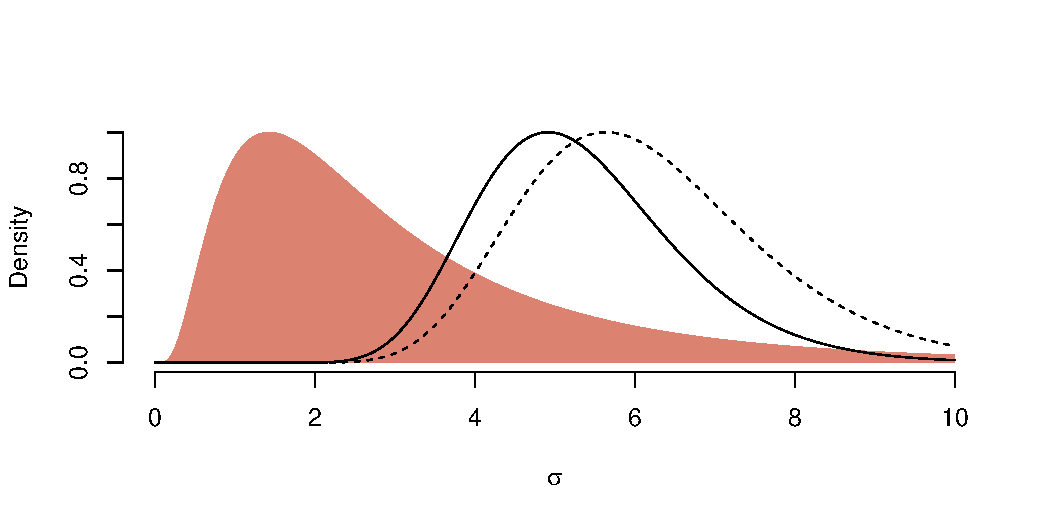
\includegraphics[width=\maxwidth]{figure/unnamed-chunk-12-1} 

\end{knitrout}
\caption{A simplified example of the basic concepts of Bayesian inference. The shaded area represents prior knowledge about the parameter $\sigma$. Dashed line is $P(Data | \theta)$ and the solid line is the posterior probability density, $P(\theta | Data)$}
\label{fig:priorpost}
\end{figure}

How the prior distribution is determined is a complex question. First of all, the prior distribution should take into account mathematical constraints, for example here the fact that $\sigma$ must always be positive, which is why I used the log-normal distribution in the example. Another aspect is that one can encode current knowledge in a meaningful way by choosing the prior appropriately. A \textit{weak} or \textit{non-informative} prior mostly acts as a way of regularizing the inferences and increasing computational stability, while a textit{strong} or \textit{informative} prior can encode specific subject-matter knowledge (for accessible discussion on priors and discussion on weak and strong priors see \citet{prior_choice_recommendations}). 

For determining priors for psychometric functions \citet{lee2018} recommends informative priors, and using prior predictive distributions--that is, distributions of psychometric functions--as a way of checking that the priors make sense and lead to psychometric functions that are realistic. One problem with this approach is that usually priors that assume independence among the parameters are used (an issue that is also discussed in \citet{prior_choice_recommendations}), but it is likely that the parameters of the psychometric functions have strong correlations between them. 

For example psychometric functions with high values for $\sigma$ but low values for $\beta$ produce psychometric functions that can be unrealistically slow in reaching high performance levels, especially if values for $\kappa_{\mu}$ or $\kappa_{\sigma}$ parameters are significantly large. The issue of encoding such dependencies in the prior is left for future work, I will be using priors which are independent out of convenience, and choosing values that make sense for the parameters in isolation, which is admittedly not optimal.  

Lastly, one particularly useful feature of priors is that it's easy to expand models into having a multilevel structure through them, which will be discussed in more detail in the next section.  

Of course, in models of any complexity prior and posterior probability densities are defined over a multidimensional space, e.g. in this thesis the dimensionalities range from 7 to 27. This means that we are not interested in, for example, probabilities for values of $\sigma$ parameter alone but probabilities for combinations of parameter values, for example, that $\sigma = 2.0$ and $\beta = 0.7$ and $\kappa_{\mu} = 0.1$ and so on for all of the parameters of the specific model.

Often it is useful to summarize multidimensional posterior density as its marginals. Most analyses done in this thesis will use the marginals of  the posterior probability densities somehow. Figure \ref{fig:marginals} demonstrates the relationship between a two-dimensional posterior probability density and its margins. The leftmost panel shows the two-dimensional distribution from above, and the two other figures show its marginals, which in this case correspond to viewing the two-dimensional "bump" from either axis. 

\begin{figure}
\centering
\begin{knitrout}
\definecolor{shadecolor}{rgb}{0.969, 0.969, 0.969}\color{fgcolor}
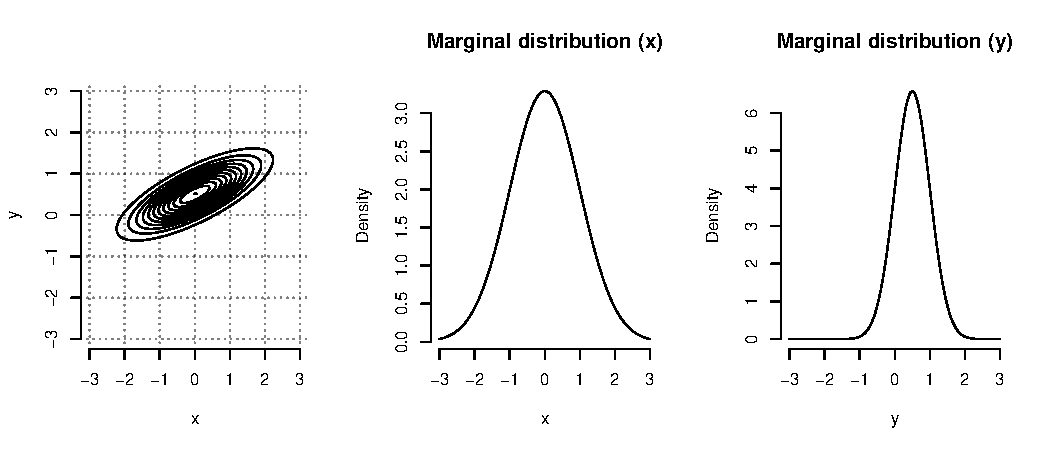
\includegraphics[width=\maxwidth]{figure/unnamed-chunk-13-1} 

\end{knitrout}
\caption{A two-dimensional posterior probability density and its marginals. }
\label{fig:marginals}
\end{figure}

\subsection{Hierarchical models}
\label{sec:hierarchical_models}

The term \textit{hierarchical model} can refer to many different kinds of models\footnote{Andrew Gelman has collected a bunch of different names for hierarchical models in to a blog post: https://statmodeling.stat.columbia.edu/2019/09/18/all-the-names-for-hierarchical-and-multilevel-modeling/ -- a fact which highlights the multifacetedness of hierarchical models}. I will be using two kinds of hierarchical models: 1) Model in which the parameters are assigned distributions 2) Models embedded in a higher level mixture model. Both kinds of models will be discussed separately.

\subsubsection*{Models in which parameters have distributions}

Often these kinds of models are described as being models in which priors have (hyper)priors (e.g. \citet[p. 225]{kruschke2015} talks about \textit{". . . hierarchical chain of dependencies among parameters."}). However, I think it's clearer to think this as an extension of fitting e.g. separate linear models to different data sets: instead it is possible to the individual linear models together on a higher level, and assign the groups of parameters (e.g. all intercepts for all of the models) distributions. This is sometimes known has \textit{random effects modelling} in the frequentist setting.

The general idea is demonstrated in Figure \ref{fig:hierarchical_model_for_groups}. The index $i$ is an index for the \textit{group} to which the observation $y_{ij}$ belongs to, $j$ indexes observations inside that group. Each observation is assumed to be drawn from a normal distribution, but each group gets a unique set of parameters of the linear model, i.e. there are as many $\alpha$ and $\beta$ as there are groups. Without the the hierarchical structure this would simply correspond to as many separate linear models as there are groups.  

Here, however, these parameters are each assigned a distribution (prior), which in this case is the normal distribution, whose parameters are unknown and are inferred from the data. Note that for the $\sigma$ parameters the normal distributions are truncated at zero. At the highest level each parameter of these distributions gets a hyperprior, which in this case for each parameter is the standard normal distribution--taking into account again that $\sigma$ is truncated at zero.

\begin{figure}[!htb]
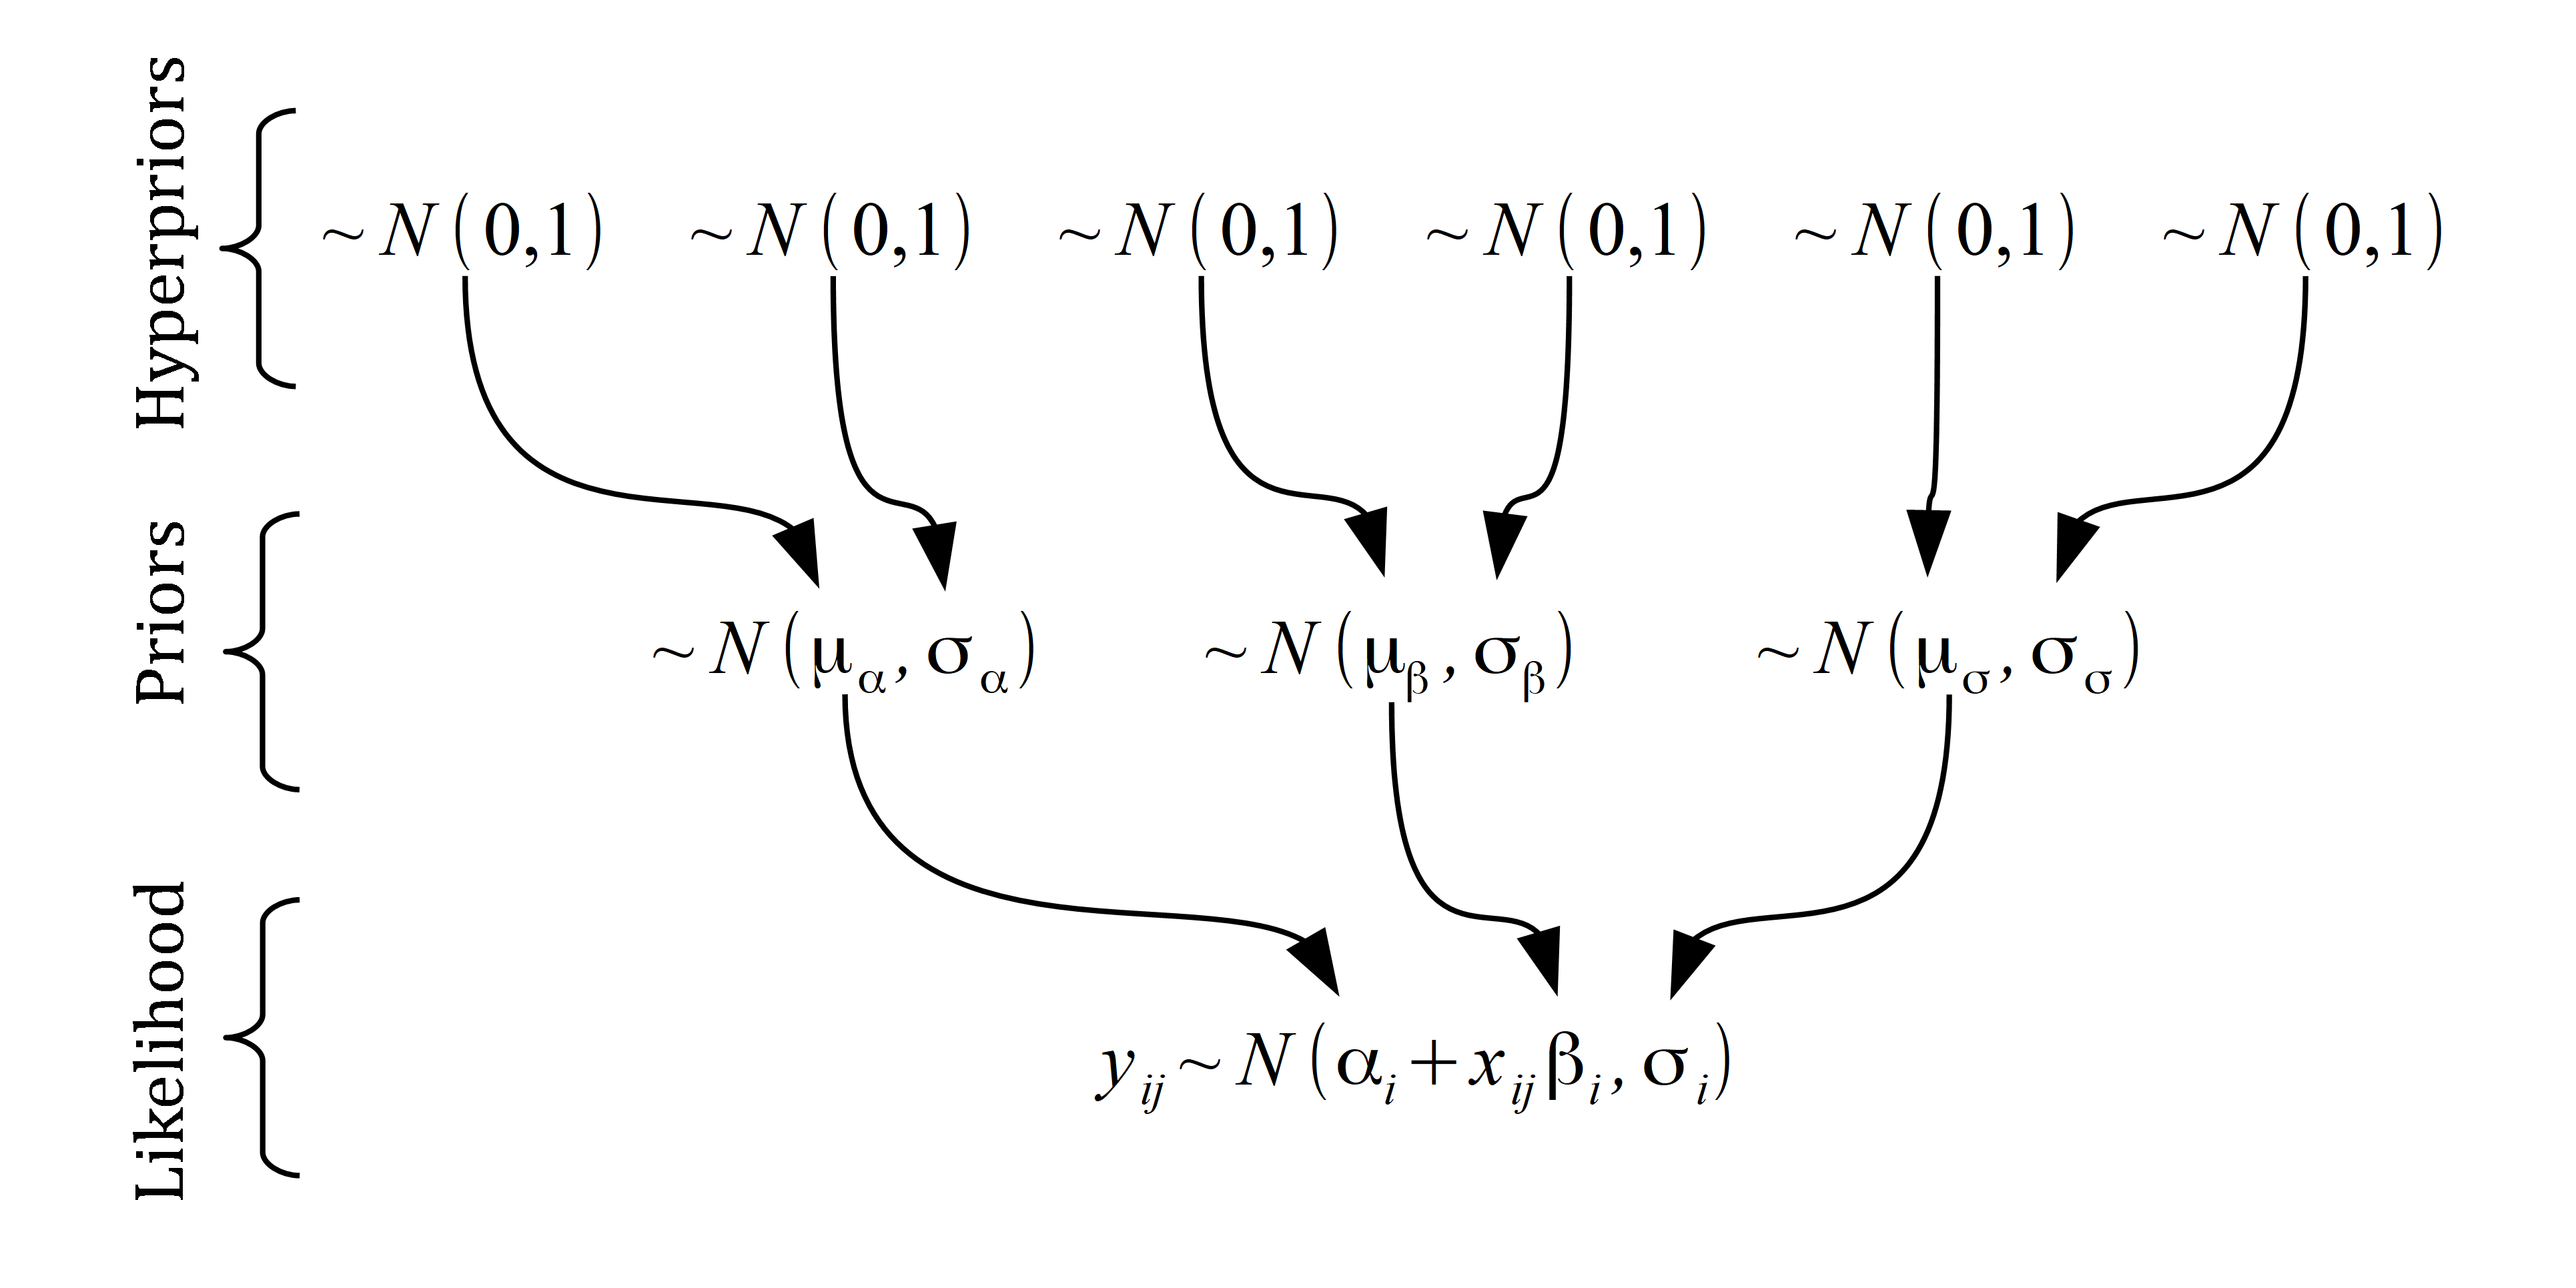
\includegraphics{Hierarchical_model_for_groups}
\caption{A schematic illustration of a hierarchical linear model in which each of the parameters is given a distribution for which the parameters are inferred from the data. This creates a distinct multilevel structure to the model.}
\label{fig:hierarchical_model_for_groups}
\end{figure}

In other words, there are--for example--separate $\alpha$ parameters for each group, but \textit{at the same time} as the values\footnote{To be precise, not \textit{values} but posterior distributions, as was discussed earlier.} for the individual $\alpha$ parameters are found, the parameters for the prior distribution from which they are assumed to be drawn from are also found; in this way the individual parameters depend on the priors, and  the parameters of the priors depend on the individual values.

Since the parameters are related on a higher level, some information is shared between them. One feature is that all of the means are adjusted towards the common mean, which functions analogously to multiple comparisons adjustments in frequentist statistics \citep{gelman2012}, which is the main reason for including the hierarchical structure here. 

\subsubsection*{Models embedded in a mixture model} 

Often the same data set can be fit by multiple models, or there are many plausible candidates for models of for the cognitive processes of interest. These are often also called \textit{mixture} models, since the idea is to model observed data as a mixture of the different models (for the general statistical idea see \citet{keller2018}). Since the individual models are embedded in a larger scale structure that models the mixing proportions, this kind of model is naturally also thought of as a hierarchical model (see \citet[Chapter 10]{kruschke2015}).

The simple two-level model I describe corresponds with how lapsing behaviour is often modelled in the psychophysical literature (see e.g. \citet{zeigenfuse2010} for a theoretical summary or e.g \citet{lesmes2015} for a practical implementation). The model is presented in figure \ref{fig:Basic_hierarchical_model}. At the lowest level, the figure shows two models, one labelled \textit{lapses} and the other \textit{cognitive}, embedded in the higher level model. Both of the lower level models aim to explain the same set of observations, $y_1, y_2 \dots y_i$, the $y$ terms, in this case, consisting of pairs of stimuli ($\bm{S} = [S_x, S_y]$) and responses ($\bm{R} = [R_x, R_y]$). 

\begin{figure}[!htb]
\begin{center}
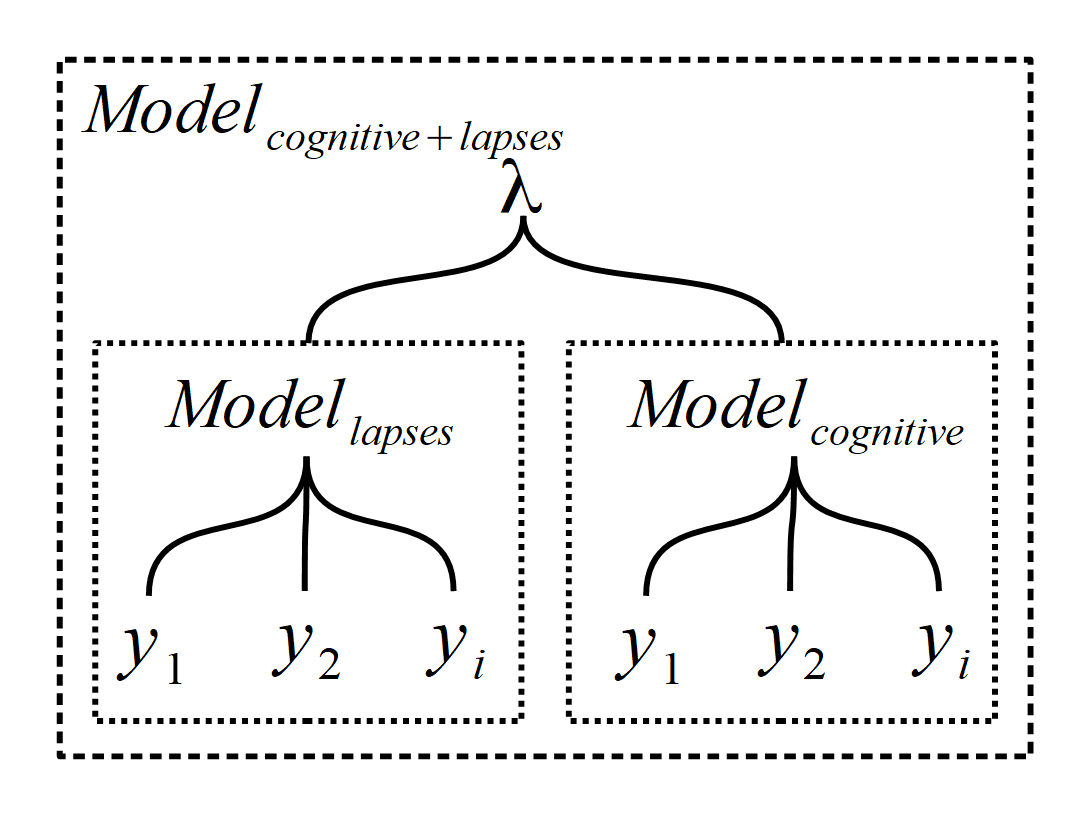
\includegraphics[scale=0.75]{Basic_hierarchical_mixture_model}
\end{center}
\caption{A simple hierarchical model, which shows how the two models, one modelling lapses and the other the cognitive processes of interest, are related on a higher level through the coefficient $\lambda$.}
\label{fig:Basic_hierarchical_model}
\end{figure}

The cognitive model can be any of the models defined in Section \ref{sec:grt_mdls} \textit{\nameref{sec:grt_mdls}}. The lapsing model (which was discussed in general terms in Section \ref{sec:lapses_general} \textit{\nameref{sec:lapses_general}}) is defined by the single parameter $\gamma$, which is a multinomial distribution containing the response probabilities for the individual response categories. These probabilities do not depend on the signal levels, or in fact, on anything else outside them (see Section \ref{sec:modelling_responses} \textit{\nameref{sec:modelling_responses}} for how the responses are coded):

\begin{equation}
P(y_i)=
\begin{cases}
  \gamma_1, & \text{if } \bm{R} = [-1, -1]\\
  \gamma_2, & \text{if } \bm{R} = [\phantom{-}1, -1]\\
  \gamma_3, & \text{if } \bm{R} = [-1, \phantom{-}1]\\
  \gamma_4, & \text{if } \bm{R} = [\phantom{-}1, \phantom{-}1]
\end{cases}
\end{equation}

This simply says that if, for example, on a certain trial the response $[1,-1]$ is observed, the likelihood is incremented by $\gamma_2$. I will be assuming that all responses are as likely, i.e. $\gamma = [0.25, 0.25, 0.25, 0.25]$. This implies that the parameters of the lapsing model are not inferred from the data, partially due to the aforementioned (see Section \ref{sec:lapses_general} \textit{\nameref{sec:lapses_general}}) difficulty of inferring details of lapsing behaviour from psychophysical data. 

The contributions of these two models are defined by the coefficient $\lambda$, which defines the weight of each model to the total likelihood:

\begin{multline}
\label{eq:lower_level_hiera}
P(y_i |\Theta_{\text{cognitive + lapses}}, \text{Model}_{\text{cognitive + lapses}}) = \lambda P(y_i | \theta_{\text{lapsing}}, \text{Model}_{\text{lapsing}}) + \\ (1 - \lambda) P(y_i | \theta_{\text{cognitive}}, \text{Model}_{\text{cognitive}})
\end{multline}

The vector $\Theta_{\text{cognitive + lapses}}$ contains all of the parameters for the lower level models and $\lambda$: $\Theta_{\text{cognitive + lapses}} = [\lambda, \theta_{\text{lapsing}}, \theta_{\text{cognitive}}]$.

\subsection{Approximating the Posterior Probability Densities}
\label{sec:posterior_approx}

One issues in doing Bayesian inference is how to calculate the posterior probability densities. Unfortunately analytical solutions are not available even for the simpler cases--e.g. one-dimensional psychometric functions--and no such solution will be developed in this thesis. \citet{kontsevichtyler1999} used \textit{grid approximation} which is based on dividing the effective range of the posterior distribution into equally spaced intervals and then calculating posterior probability density at each point (see \citealt[p.144]{kruschke2015}). The downside is that this method becomes computationally costly when dealing with high dimensional posterior distributions. E.g. if one has a 9-dimensional posterior distribution--like in the present case--and wishes to represent it with even 25 discrete points per dimension, one would need to calculate $25^9$ values, which is infeasible even given the computing capabilities of modern computers.

To circumvent this problem, three approximation methods were used in different parts of this thesis. For fitting models to already collected data, the models implemented in Stan programming language. For the adaptive algorithm to work, on each trial one needs approximate the current posterior probability density in (close to) real time, for this reason Resample-Move algorithm and Laplace approximation were used there. I will describe the Resample-Move algorithm and Laplace approximation in more detail, since they have direct consequences on the implementation of the adaptive algorithm; sampling methods used by Stan are taken \textit{as is}. It suffices to say that similar to the Resample-Move algorithm to be described shortly, Stan uses random numbers to approximate the posterior distribution and these random numbers are generated by Markov Chain Monte Carlo methods (\citet[Chapters 15 \& 16]{stan_manual_new}; for the general principle of approximating posterior distributions with random sampling see \citet[Chapter 7]{kruschke2015}).

\subsubsection{Resample-Move algorithm}

The Resample-Move algorithm, as described by \citet{chopin2002} involves using \textit{sequential importance sampling} and the occasional \textit{rejuvenation} step (see Algorithm \ref{alg:resamplemove}).  

Central idea is to represent the posterior distribution as \textit{random samples} from it. This is demonstrated in the left panel of Figure \ref{fig:degeneracy}, in which a one-dimensional normal distribution, as represented by the solid line, is approximated with a set of uniformly sampled values along the $x$-axis, called particles. The heights of the particles (the dashed lines) correspond to the weights of the particles (proportionally; the weights should always sum to unity). One can use the values and weights to estimate e.g. the mean and variance of the underlying distribution, using standard formulae for discrete random variables.

\begin{algorithm}
\caption{Sequential importance sampling with rejuvenation}
\label{alg:resamplemove}
\begin{algorithmic}[1]

\State At the beginning of the experiment, draw $N$ particles from the prior distribution and set uniform weights.
\State Observe a data point.
\State Update the particle weights according to the observation.
\If {$N_{\text{eff}} < N/4$}
        \State Resample particles.
        \State Move resampled particles.
    \EndIf
\State Return to step 2.

\end{algorithmic}
\end{algorithm}

\begin{figure}[!htb]
\begin{center}
\begin{knitrout}
\definecolor{shadecolor}{rgb}{0.969, 0.969, 0.969}\color{fgcolor}
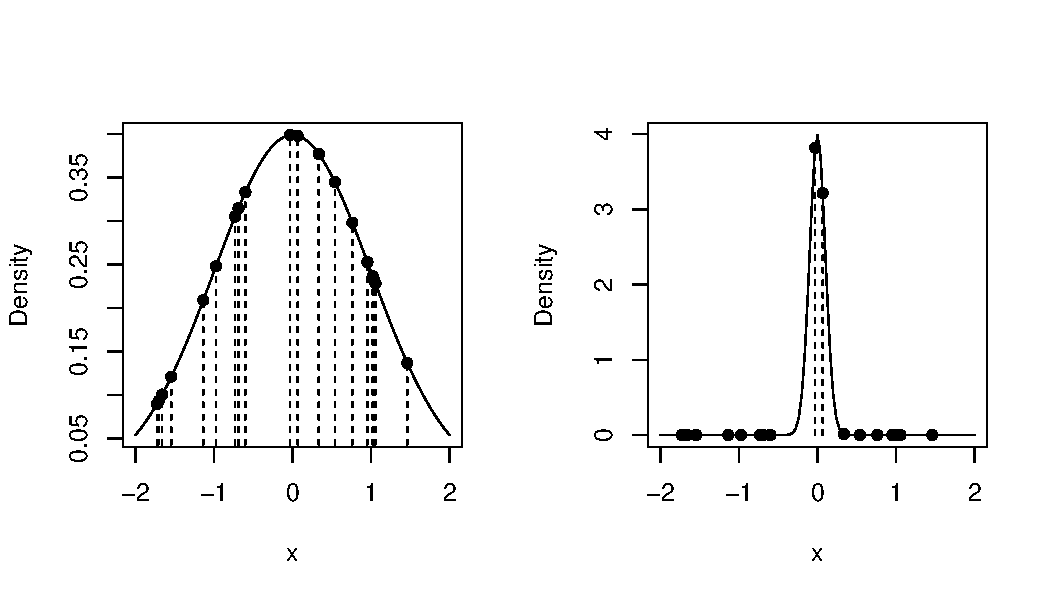
\includegraphics[width=\maxwidth]{figure/degeneracy-1} 

\end{knitrout}
\end{center}
\caption{ Demonstration of sequential importance sampling and particle degeneracy. When the posterior probability becomes more concentrated, after some data is observed, less particles have weights that differ significantly from zero. }
\label{fig:degeneracy}
\end{figure}

The complete particle sets thus is most conveniently thought of as a matrix with parameter values and their weights. Table \ref{table:particleSet} demonstrates this idea for the 2I-4AFC model. The particle set consists of randomly sampled values of the parameters, $\theta$. Each row corresponds with one set of parameter values and a weight, $w$. In Figure \ref{fig:degeneracy} weights were shown for a single parameter, here weights correspond with their "heights" in a 7-dimensional space. 

\begin{table}[!htb]
\centering
\caption{An example of a particle set, which consists of sets of parameter values, $\theta$, and associated weights.}
\vspace{0.5cm}
\label{table:particleSet}
\begin{tabular}{ccccccccc}
\toprule

& \multicolumn{7}{c}{$\theta$}    \\
\cmidrule(lr){2-8}
& $\sigma_x$  & $\sigma_y$  & $\beta_x$   & $\beta_y$   & $\kappa_x$ & $\kappa_y$ & $\rho$   & $w$  \\
\midrule
1    & 1.2  &  2.5 &  0.2 & 2.6 & -0.2 & 0.5 & -0.1 & 0.10 \\
2    & 0.5  &  0.3 &  1.1 & 0.6 &  0.4 & 0.1 & 0.2 & 0.05 \\
3    & 0.2  &  1.7 &  1.8 & 1.5 &  0.3 & -0.1 & 0.3 & 0.15 \\
\vdots & \vdots  &  \vdots &  \vdots & \vdots & \vdots  & \vdots & \vdots  & \vdots  \\
$N$  & 0.4  &  1.5 &  0.7 & 0.8 & -0.1 & -0.5& 0.75 & 0.20 \\
\bottomrule
\end{tabular}
\end{table}

As more data is observed, fewer and fewer particles have non-zero weights. This is natural, since usually at the beginning of an experiment there's more uncertainty about the specific values of the parameters, but as the experiment progresses, more and more particles can be singled out, or given smaller weights. When the underlying distribution becomes more concentrated, the weights of most particles approach zero, as is shown in Figure \ref{fig:degeneracy}). This is called \textit{particle degeneracy}. A simple way of quantifying it is the effective sample size \citep{speekenbrink2016}:

\begin{equation}
N_{\text{eff}} = 1 / \sum_{i}^{N} w_i^2
\end{equation}

When the particle set becomes too degenerated--here defined as the point when $N_{\text{eff}} < N/4$--it has to be rejuvenated. 

Rejuvenation is done by first resampling the particles. Resampling means sampling new particles with replacement proportional to their weights. I used \textit{multinomial resampling}. This is similar to how a roulette wheel works, the difference being that in a roulette wheel each number has a uniform probability of being chosen; here the "sectors" for some particles are wider, and thus they have greater chance of being chosen. This results in particles with greater weights being replicated, and particles with lower weights being removed from the particle set. This does not effectively combat particle degeneracy which is why the algorithm has a \textit{move} step. \citep{chopin2002}

During the move step proposed particles are drawn from what is called a \textit{proposal distribution}. As the proposal distribution I used a multivariate normal distribution with means and standard deviations corresponding to those of the current posterior distribution, as suggested by Chopin. These proposals are accepted with the probability: $p(\text{proposal}_i | y) / p(\text{old particle}_i | y)$, that is the ratio of the posterior probabilities of an old particle and a proposed particle. It is easy to see that for proposals, which have higher posterior probability than the old particles, the probability is greater than one, implying that they are always accepted. \citep{chopin2002}. 

Particle methods have been used in adaptive estimation for example by \citet{dimattina2015}, although they did not implement the rejuvenation step, making their implementation unrealistic for the longer experimental runs used here, and by  \citet{kujalalukka2006} who use a more sophisticated  rejuvenation step, which, due to its increased computational cost, was also not realistic. 

\subsubsection{Laplace Approximation}

In Laplace approximation one finds the maximum of the posterior distribution, and by calculating the second derivatives at that point estimates it's marginal standard deviations and correlations--called the Hessian matrix. The posterior distribution can then be represented by a multivariate normal distribution whose mean is the maximum and covariance matrix is calculated from the Hessian matrix. For example citet{shen2013} uses Laplace approximation for adaptively estimating auditory filters.

Given the reparametrisation at the end of this section, this could possibly be a reasonable way of approximating the  posterior, however in my experience the posterior distribution does sometimes have markedly non-linear dependencies among the parameters, and these are not captured well by Laplace approximation. For this reason Laplace approximation was used in this thesis just as a backup--see \ref{sec:practical_considerations} \textit{\nameref{sec:practical_considerations}}.

\subsection{Bayesian inference in the General Recognition Theory}

In this work Bayesian approach is also used during the analysis of the data. Classic GRT studies have been dominated by frequentist methods, and e.g. definitions of interactions have relied on testing for the statistical significance of the parameter values associated with them (e.g. \cite{ashby2015, wickens1992}), to my knowledge, \cite{silbert2010} is the only GRT related work using Bayesian analysis framework. Contrary to the majority of studies, I won't be doing any explicit significance tests, nor am I using the usual \textit{Type I/II} error framework \citep[pp. 470 - 471]{christensen1997}, since there are many problems associated with this.

For example if interactions are selected based on their statistical significance, effect sizes are likely to be exaggerated \citep{gelman2018}; but the more damning criticism is that the $p$-value doesn't differentiate between \textit{effect} or \textit{no effect} (\cite{greenland2016}), i.e. between \textit{interaction} or \textit{no interaction}, and in general, there has been a substantial amounts of criticism targeted towards focusing on binary decisions based on \textit{p}-values and instead a push to instead focus on the effect sizes and uncertainties associated with them (see e.g. \citet{kline2004, greenland2016, steiger1997}). 

This shift should not be seen only as a trivial data analytical decision: it should be seen as reflecting a wider push in the behavioural sciences to move away from binary decisions (see e.g. \citet{amrhein2017}), and--in the light of the topic--relating to the interpretation of interactions as being graded properties of the stimuli (as discussed in \citet{kemler1993}), instead of something that either is or isn't. On the other hand, in Null Hypothesis Testing (NHST, see \citet[Chapter 11]{kruschke2015}), as it is usually implemented, the main goal is to reject some uninteresting default model, while in Bayesian analysis--as it's defined in \citet{bda}--the explicit goal is to develop models that describe the data generating processes realistically. I find this goal to be much intuitively meaningful--rejecting an uninteresting default model only tells us that the specific model is bad, it does not tell us what models are good. In GRT this usually means rejecting some model that assumes no interactions between the dimensions--the important question of \textit{what kind} of interactions there then actually are can't be reliably answered by just using NHST.

\paragraph{Posterior predictive checks}

An important part of Bayesian work flow is \textit{model critique}. The starting point is the boxian philosophy that \textit{"All models are wrong . . ."} \citep{box2005}: since we can be a priori certain that all models are wrong to a degree, it becomes important to check the model against the data to see \textit{how} it is wrong, and if the mismatch is significant. This kind of \textit{model criticism} is an integral part of Bayesian workflow, as described e.g. in \citet[Part II]{bda}.

In the classical GRT models, model checking has usually been limited to comparing the predicted response probabilities with the observed probabilities (see for example \citet[Figure 4]{silbert2009}).  However this suffers from the fact that, as discussed earlier in Section \ref{sec:grt_criticism} \textit{\nameref{sec:grt_criticism}}, the classic GRT models are prone to over-fitting, which means that the predicted response probabilities will \textit{always} be fairly close to the observed probabilities. This not evidence for the theoretical assumptions behind the model, but rather just an artefact of the flexibility of the model.

In Bayesian setting, \textit{posterior predictive checks} can be used to assess the fit of the model to the data. The idea is to use the posterior distribution to predict new data. The distribution of predicted data can be thought of has what the model "thinks" about the data. If there's large discrepancies between what the model thinks and data, this is a clear indication that the model does not sufficiently capture all relevant features of the data. \citep[Chapter 7]{bda}.

Developing good posterior predictive checks can be difficult, and there is not a set way to conduct them. In this thesis I will be using simple checks that are based on dividing the data into discrete categories and counting the number of positive responses in each category. This is not exhaustive, but, as will be seen in the analysis section, is sufficient for some making some preliminary observations. 

\paragraph{Unconstrained parameterization}

By their very nature, $\sigma$ parameters are bound to be positive, since they represent standard deviations. The $\beta$ terms don't have to be positive, but since the psychometric functions are assumed to be monotonically increasing, I restricted the $\beta$ parameters to be positive too. The correlation parameter, $\rho$, is bound between -1 and 1. 

As already mentioned, these bounds have to be taken into account when deciding what distributions to use as prior distributions for the parameters. One solution is to choose distributions with matching supports, i.e. for example log-normal distributions for the parameters bound to positive real numbers. Another possibility is to \textit{reparametrise} the model in such a way that some convenient distributions can be used. The latter approach is taken here. 

Priors for $\sigma$ and $\beta$--and as a consequence the parameters themselves--are defined on the logarithmic scale. Prior for $\rho$ is defined on the inverse hyperbolic tangent scale. Both of these are widely used transformations in statistics for these kinds of situations (see \citet[Chapter 22]{stan_manual}). In practice this means  that the \textit{inverse} transformations have to be implemented in the likelihood calculations.

For the $d'$ calculations this implies that Equation \ref{eq:twodimdprime} becomes

\begin{align}
\begin{split}
d'_x &= (\frac{S_x}{exp(\sigma_x)})^{exp(\beta_x)} + \kappa_x S_y \\
d'_y &= (\frac{S_y}{exp(\sigma_y)})^{exp(\beta_y)} + \kappa_y S_x
\end{split}
\end{align}

and for the psychometric function (compare this with Equation \ref{eq:generalPfun}):

\begin{equation}
\psi_2(\bm{S}; \theta)_{(R_x, R_y)} = \phi_2([-c_x + d'_x]r_x, [-c_y + d'_y] r_y, \text{tanh}(\rho) [r_x r_y])
\end{equation}

A similar transformation would be applied also to Equation \ref{eq:generalPfun2}.

An important aspect of this process to note is that since the priors are normal on the \textit{transformed scale}--i.e. $log\sigma \sim N(\mu, \sigma)$--, they are not normal on the \textit{original scale} (see \citealt[pp. 729 - 732]{kruschke2015}). Indeed, the current parameterization implies that for  example the prior for $\sigma$ is a log-normal distribution.

Another consequence of reparametrisation is that it makes the rejuvenation step of the particle filter slightly simpler. During the rejuvenation step new proposal particles have to be generated from some distribution. It is possible to choose an asymmetric distribution, such as the log-normal distribution, but this leads to two additional complexities: the acceptance probability is now dependent also on the proposal distribution (see ERROR) and the moments calculated from the particle set (mean and standard deviations of the particles) have to be transformed to the parameters of the non-symmetric distribution. 

On the other hand using an unbounded proposal distribution on the bounded space can lead to many proposals  being  outside the support of the distribution, reducing the efficiency of the rejuvenation step.



\newpage

%Rnw root = "../Joni_Paakko_-_Thesis.Rnw"

\section{Adaptive estimation}
\label{sec:adaptive}

The motivation behind adaptive psychophysical testing can be traced to intuitive enough starting point. Suppose that the researcher is interested in finding out what is the faintest possible sound that the subject is able to detect. It wouldn't make sense to waste time presenting them with stimuli that they can always detect, rather, if the subject has very low threshold for detection, it would make sense to reduce the level of the stimuli until the subject starts making errors, which is how adaptive \textit{staircase methods work} (c.f. \citet[Chapter 5]{kingdomprins2010}).

A popular subclass of adaptive methods are based on Bayesian statistics. \cite{watson1983} introduced the \textit{QUEST} procedure which was influential in its use of Bayesian statistics in determining which stimuli to choose. The QUEST procedure was used only for estimating one parameter, threshold (analogous to the parameter $\sigma$ in this thesis),  and it was later expanded by \citet{king_smith1997} in their ZEST algorithm for estimating the threshold and slope of the psychometric function (analogous to the parameters $\sigma$ and $\beta$ in this thesis). 

However, it wasn't until the work by \citet{kontsevichtyler1999} that Bayesian Adaptive Estimation as how it would be known today would emerge. The aforementioned QUEST and ZEST procedures used \textit{ad hoc} heuristics for determining the placement of the stimuli: in the QUEST procedure stimuli are placed near the threshold, in the ZEST procedure, in order to estimate the slope of the psychometric function, stimuli are placed above and below the threshold. 

In the procedure used by \citet{kontsevichtyler1999} stimuli that minimize the \textit{expected entropy} of the posterior distribution are chosen. In simple terms, entropy refers to the evenness of a probability distribution \citep[p. 365]{kruschke2015}. This is demonstrated in Figure \ref{fig:entropy}. The figure depicts two multinomial distributions, in which the categories refer to the possible responses for two-dimensional stimuli (see Section \ref{sec:grt_mdls} \textit{\nameref{sec:grt_mdls}}. The distribution on the left is maximally even, while the distribution on the right side has more probability assigned to the responses (0,0) and (1,1). Consequently, the distribution on the right has less entropy.

\begin{figure}
\begin{center}
\begin{knitrout}
\definecolor{shadecolor}{rgb}{0.969, 0.969, 0.969}\color{fgcolor}
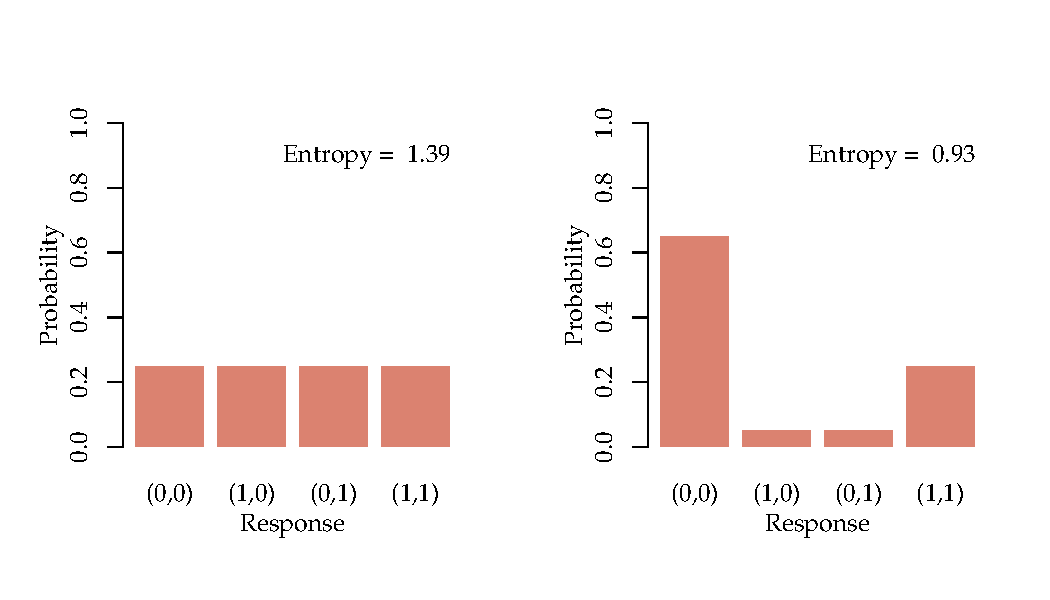
\includegraphics[width=\maxwidth]{figure/unnamed-chunk-14-1} 

\end{knitrout}
\end{center}
\caption{Two multinomial distributions that represent the probabilities for the possible response categories in the model. The distribution on the right is less even, and as a consequence has less entropy.}
\label{fig:entropy}
\end{figure}

In terms of posterior distribution this means that stimuli, that make the posterior probability densities as concentrated around a single point as possible are chosen. Recall from the previous section on Bayesian statistics that the spread of the posterior distribution for the parameters quantifies uncertainty related to the values of the parameters. Thus, minimizing the spread of the posterior entropy minimizes uncertainty about their values. 

The reason for using the distribution of responses in the above example is that \citet{kujalalukka2006} and \citet{kujala2011} show that minimizing the entropy of the response distribution is equivalent to minimizing the entropy of the posterior distribution of the parameters--which is the ultimate goal. This is, in my opinion, simpler than minimizing the entropy of the posterior distribution directly as done by \citet{kontsevichtyler1999}. Intuitively this can be understood by realizing that if there's lots of uncertainty about the parameters, this uncertainty carries over to predictions about responses (c.f. Figure \ref{fig:entropy}): all of the responses seem almost as likely. Conversely, if only very specific parameter values are, so are specific response categories too. 

\citet{kujalalukka2006} and \citet{kujala2011} give equations for calculating information gain using a set of IID particles--that is, particles with uniform weights. Since a weighted set is used here, the equations are modified to accommodate for this:

\begin{equation}
h(\sum_{i=1}^N w_i \psi_2(\bm{S};\theta_i)) - \sum_{i=1}^N h(w_i \psi_2(\bm{S};\theta_i)) 
\label{eq:infgain}
\end{equation}

in which $h$ is the entropy of a discrete distribution, in this case, a distribution the response probabilities. Each $\theta_i$ is a "slice" of the matrix of particles (a single  row of Table \ref{table:particleSet}), defining a single set of parameter values. $h$ is \citep{kontsevichtyler1999}:

\begin{equation}
h(p) = -\sum_{i = 1}^{N} p_i ln p_i
\end{equation}

On each trial the stimulus that maximizes Equation \ref{eq:infgain} is chosen. 

The allure of this method lies in that the stimulus selection heuristic is entirely based on principles of Bayesian statistics, and by that virtue entirely abstract and thus generalizable. Indeed, this principle has been applied widely in psychophysics, also to estimation of multidimensional psychometric functions. However, the approach I use differs from previous work on adaptive methods with multidimensional signals. 

In the approaches by \citet{dimattina2015}, \citet{lesmes2006}, \citet{shen2013, shen2014} and \citet{kujalalukka2006} Bernoulli distributed responses are modelled, that is, only two response categories are used. In the QUEST+ procedure introduced by \citet{watson2017} it is possible to use multinomial distribution as a model of the responses, but the approach is quite different, e.g. the correlation is not modelled and the approach is not based on GRT. 

\paragraph{Some practical considerations}
\label{sec:practical_considerations}

In the preceding discussion I described the adaptive algorithm theoretically. In implementing the algorithm in R \citep{r_language}, some practical issues came up. 

First, a look-up table of the bivariate integrals (the function $\phi_2$) was pre-computed to speed up the calculations. 

Second, maximizing the information gain function using optimization algorithms proved prohibitively slow and unreliable. For this reason the possible stimuli were chosen from a grid of 15 stimuli. This allowed me to pre-compute response probabilities for all of the stimuli, which sped up the algorithm considerably. 

Third, during the adaptive run, whenever the particle set was rejuvenated, the ranges for the grid, from which the stimuli were chosen were re-computed. The lower and upper limits for stimuli were found from inverting the $d'$ function, and then finding stimulus levels that would correspond to $d' = 0.1$ for the lower limit and $d' = 2$ for the upper limit (Equation \ref{eq:limits}). Posterior means for the $\sigma$ and $\beta$ parameters were used, in addition, to take into account posterior uncertainty, these were shifted by 1.96 standard deviations to produce psychometric functions with either steep slope (high $\beta$) and low threshold (low $\sigma$) or shallow slope and high threshold. These corresponded to the most extreme scenarios: if the observer's psychometric function has a shallow slope and high threshold, response probabilities change relatively slowly and the range of stimuli has to be larger; the inverse is true if the threshold is slow and the slope steep. 

\begin{align}
\begin{split}
\label{eq:limits}
S_{\text{lower}} &= 0.1^{(1.0 / exp(E[\beta] + 1.96 * SD[\beta])) exp(E[\sigma] - 1.96 * SD[\sigma])}
\\ 
S_{\text{higher}} &= 2.0^ {(1.0 / exp(E[\beta] - 1.96 * SD[\beta])) exp(E[\sigma] + 1.96 * SD[\sigma])}
\end{split}
\end{align}

Fourth, to ensure that the particle approximation is accurate, three parallel particle algorithms were run. If the algorithms diverged--here defined as the marginal means differing more that $.2$ on the prior scale--Laplace approximation was used to start the particle sets again.

\newpage

%!Rnw root = ../Joni_Paakko_-_Thesis.Rnw

\section{Simulations}
\label{sec:simulations}

I will be considering two main questions: 

\begin{enumerate}
  \item How much more efficient the adaptive algorithm is in relation to sampling stimuli from a fixed grid--if at all? 
  \item How well can generating parameters be recovered?
\end{enumerate}

These questions are closely related, since relative efficiency of the algorithms (Question 1) is defined here by the quantities that are also used to evaluate Question 2. 

There are two quantities of interest. First is defined by taking the means of the marginal posterior distributions as point estimates and calculating the squared differences to the generating parameters. This quantifies squared bias and variance of these estimators. The second quantity is the standard deviations of the marginal posterior distributions. This is used as a measure of how much uncertainty about the parameters is left after the data collection process. The goal, as already stated, is to minimize uncertainty about the parameters.

Question 1 is evaluated by inspecting if there are differences between the algorithms in how quickly the aforementioned quantities approach zero. Question 2 is answered by looking at the same  quantities, but the focus is on the overall performance, not differences. The first question is more closely related to the topic of this thesis, but the second question has more general value regarding the estimation of GRT models for which reason it can't be ignored. 

\subsection{Methods}

The general method was the following: first a set of generating parameters for the simulated observer were drawn randomly, and then either of the algorithms (adaptive/non-adaptive) described earlier were run. This was done for both the Yes/No and 21-4AFC procedure, resulting in four different conditions. I have chosen the number 800 fairly arbitrarily; it represents a number of trials that, I think, could still be administered relatively continuously to a participant, without taking into account non-stationarities induced by a multi-session design\footnote{This was the number of trials completed by both participants during one session of the psychophysical experiment conducted for this thesis, see Section \ref{sec:pp_exp} \textit{\nameref{sec:pp_exp}}}. 

\paragraph{Prior distributions}

Prior distributions and distributions from which generating parameters for the simulations were drawn from are shown in Figure \ref{fig:priors} and in tabular form in Table \ref{tab:priors}. The same prior and generating distribution is used for both dimensions. Note that the scale for criterion is given in false alarm probabilities for easier interpretation. 

Priors for the parameters were chosen based on prior information from \citet{silbert2009} and from pilot testing. 

Prior for $\sigma$ was chosen to be fairly vague to reflect the possibility of widely differing thresholds.

Generating parameters for the simulations were drawn from bimodal distributions. The idea was to draw values that are covered by the prior, but which do not necessarily correspond with the mode of the prior distribution. Another motivation was to have qualitatively different simulated observers: some that have high values for some of the parameters and others that have low values.

\begin{figure}[!htb]
\centering
\begin{knitrout}
\definecolor{shadecolor}{rgb}{0.969, 0.969, 0.969}\color{fgcolor}
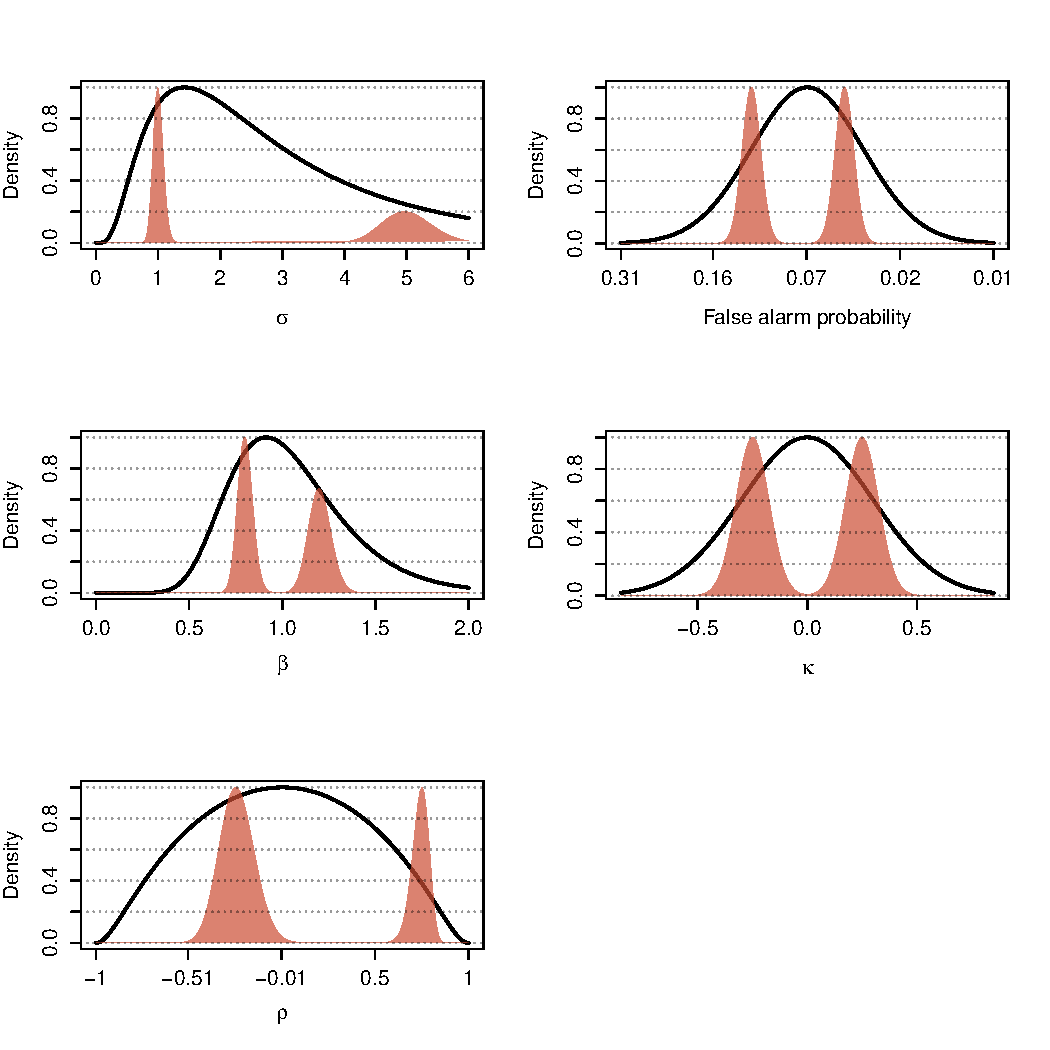
\includegraphics[width=\maxwidth]{figure/unnamed-chunk-15-1} 

\end{knitrout}

\caption{Prior distributions for the parameters of the model (solid black lines) and distributions for generating parameters for the simulations (regions shaded with red). Note that all of the densities are normalized to have maximum value of 1.0.}
\label{fig:priors}
\end{figure}

\begin{table}[H]
\centering
\caption{Parameters used for prior distributions and distributions of generating parameters. $M^l$ and $M^u$, respectively, are for the lower and upper peaks of bimodal distributions.}
\vspace{0.5cm}
\begin{tabular}{cccccc}
\toprule

          & \multicolumn{2}{c}{Prior} & \multicolumn{3}{c}{Generating}   \\
          \cmidrule(lr){2-3}\cmidrule(lr){4-6}
          & $M$       & $SD$    & $M^l$         & $M^u$         & $SD$   \\
\midrule
$\sigma$  & $log(2.5)$  & $0.75$   & $log(1)$    & $log(5)$    & $0.08$ \\
$C$       & $1.5$            & $0.3$   & $1.2$         & $1.7$         & $0.05$  \\
$\beta$   & $log(1)$  & $0.3$   & $log(0.8)$    & $log(1.2)$    & $0.05$ \\
$\kappa$  & $0$            & $0.3$   & $-0.25$        & $0.25$         & $0.075$ \\
$\rho$    & $0$            & $0.7$  & $atanh(0.75)$ & $atanh(-0.25)$  & $0.1$ \\
\bottomrule
\end{tabular}
\label{tab:priors}
\end{table}

\subsection{Results}

Total number of simulations per condition are shown in Table \ref{tab:conditions}. Squared errors and marginal standard deviations are presented in two ways: 1) on trial-by-trial basis and 2) by estimating the average differences on the last trial.

\begin{table}[H]
\centering
\caption{Conditions and number of simulations in each.}
\vspace{0.5cm}
\begin{tabular}{ccc}

\toprule
Procedure & Algorithm & N \\
\midrule
Yes/No & Adaptive & 184 \\
Yes/No & Random & 284 \\
2I-4AFC & Adaptive & 174 \\
2I-4AFC & Random & 130 \\

\bottomrule

\end{tabular}

\label{tab:conditions}
\end{table}

\paragraph{Trial-by-trial estimates}
Trial-by-trial results from the simulations are summarized in Figures \ref{fig:simulation_YN_sensory_sq_error} to \ref{fig:simulation_AFC_interaction_SD}. The figures show squared errors in relation to generating parameters and marginal standard deviations after $N$ trials, all the way to trial number 800. In all plots black color is used for the randomly sampled stimuli while red is used for adaptively sampled stimuli. The shaded regions indicate 50\%-quantiles (from 25\% to 75\%); solid lines indicate medians. Sensory ($\sigma$, $\beta$, crit) and interaction ($\kappa_{\mu}$, $\rho$) are shown in their own figures.

\begin{figure}[H]
\centering
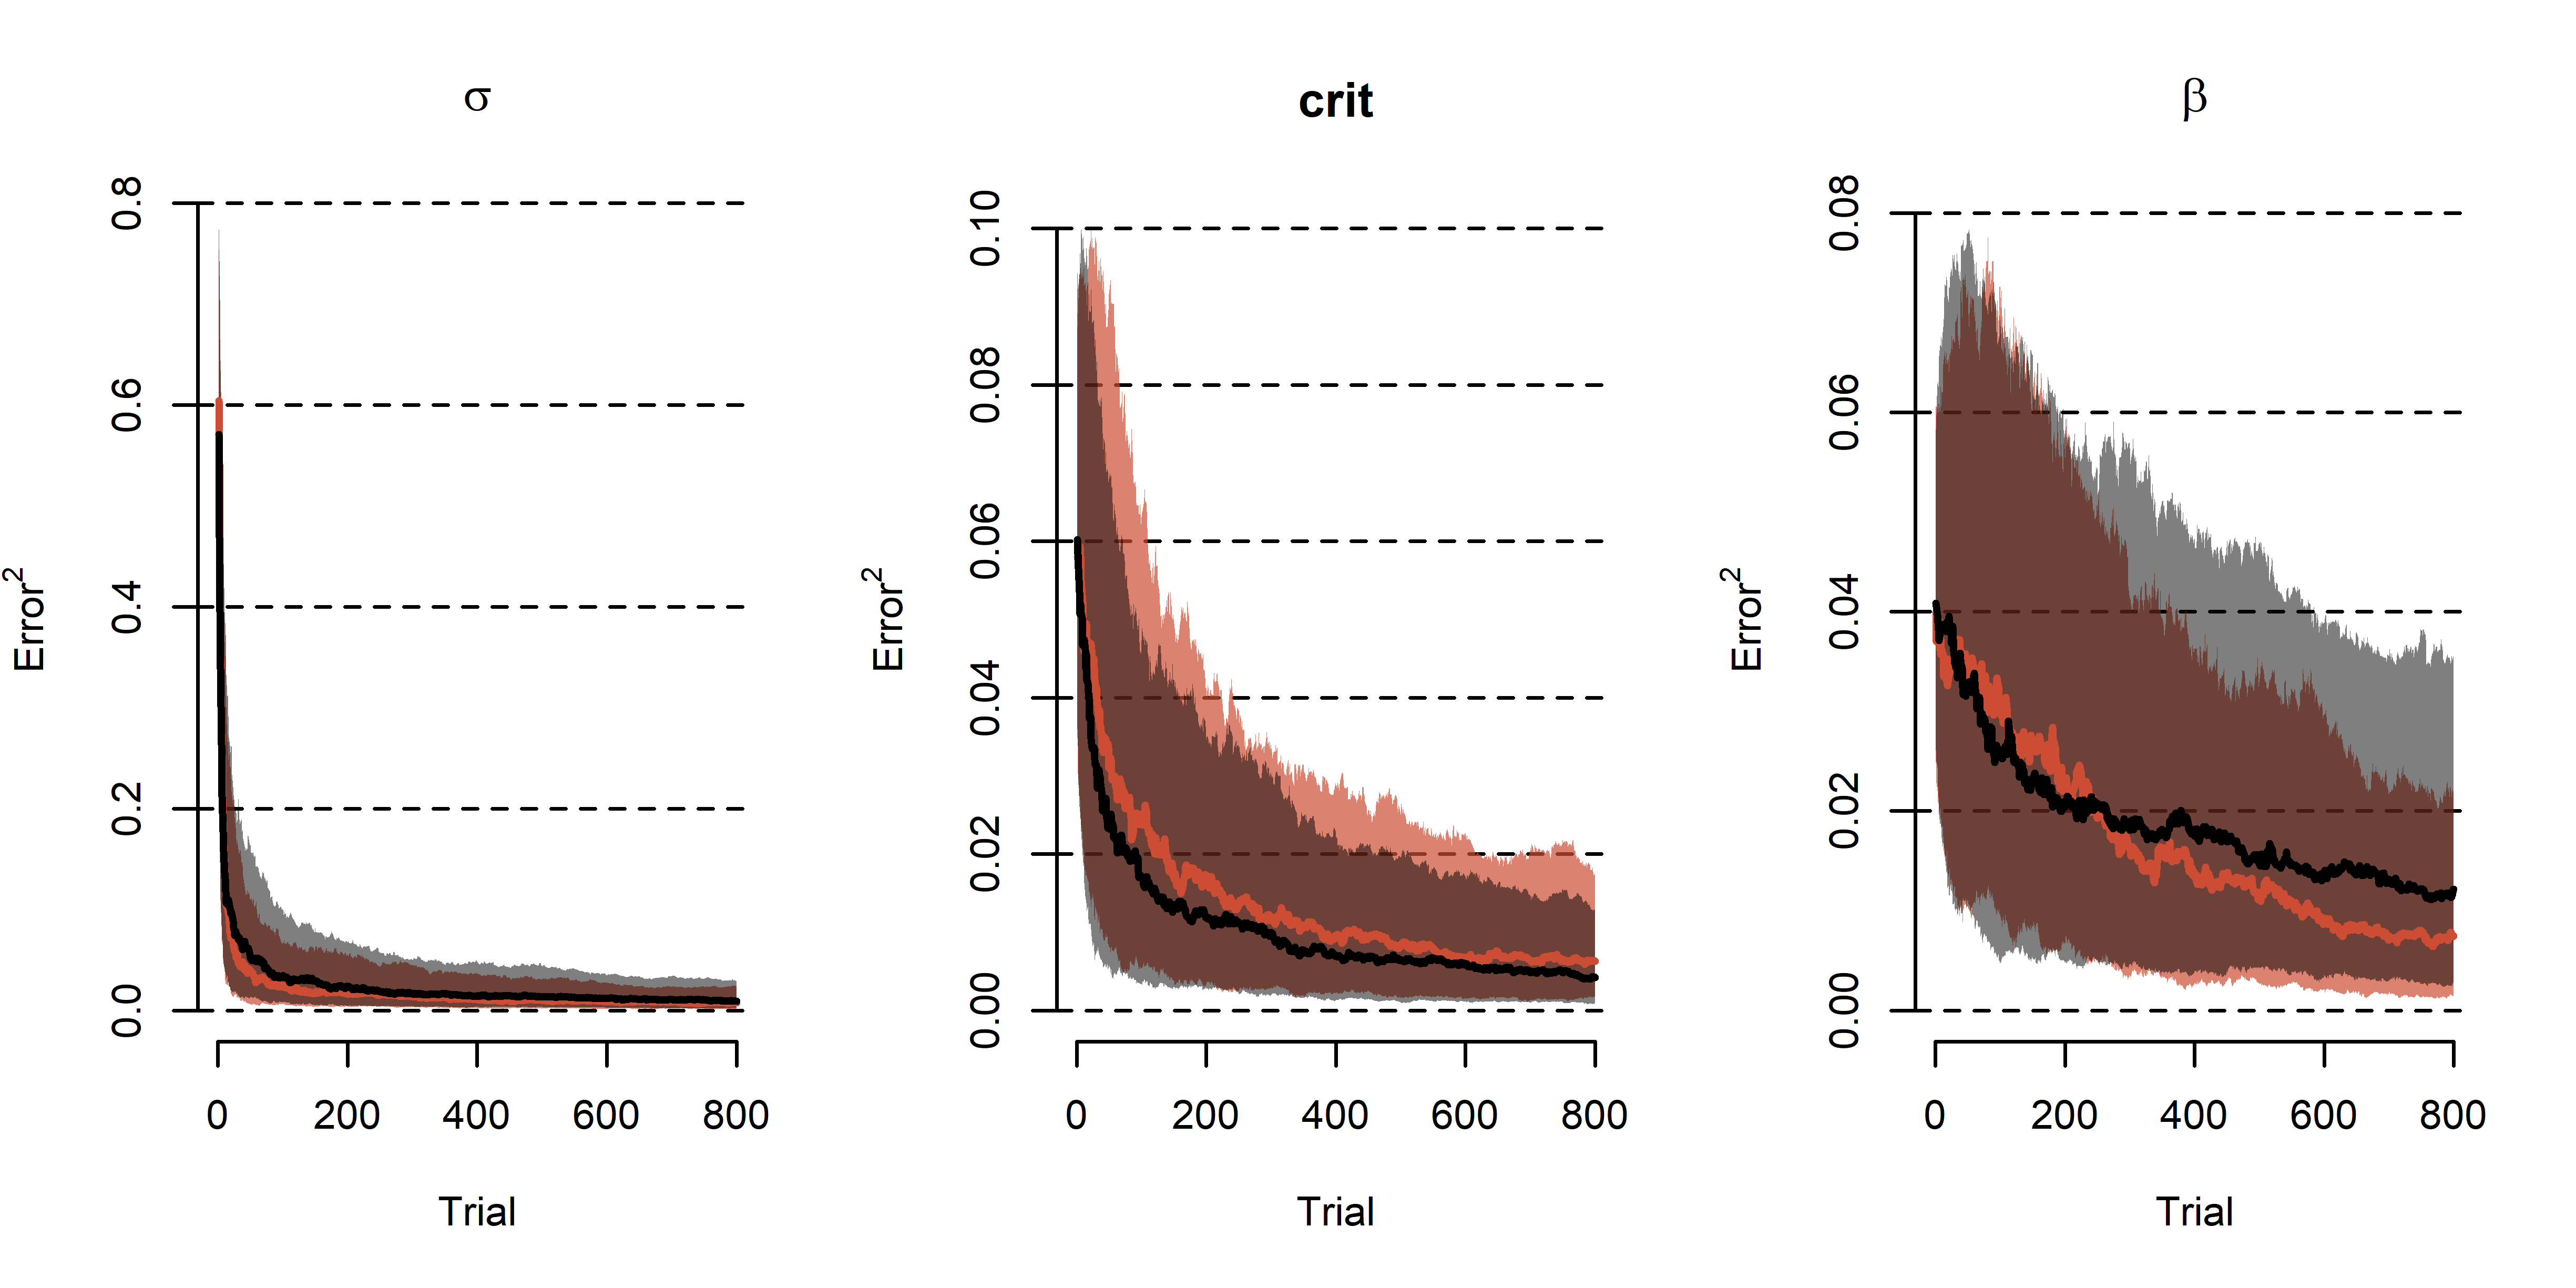
\includegraphics[scale=0.75, angle = 0]{simulation_YN_sensory_sq_error}
\caption{Procedure: Yes/No; sensory parameters. Trial-by-trial squared error between marginal means of the posterior distribution and generating parameters. Red: adaptive algorithm; black: random stimuli.}
\label{fig:simulation_YN_sensory_sq_error}
\end{figure}

\begin{figure}[H]
\centering
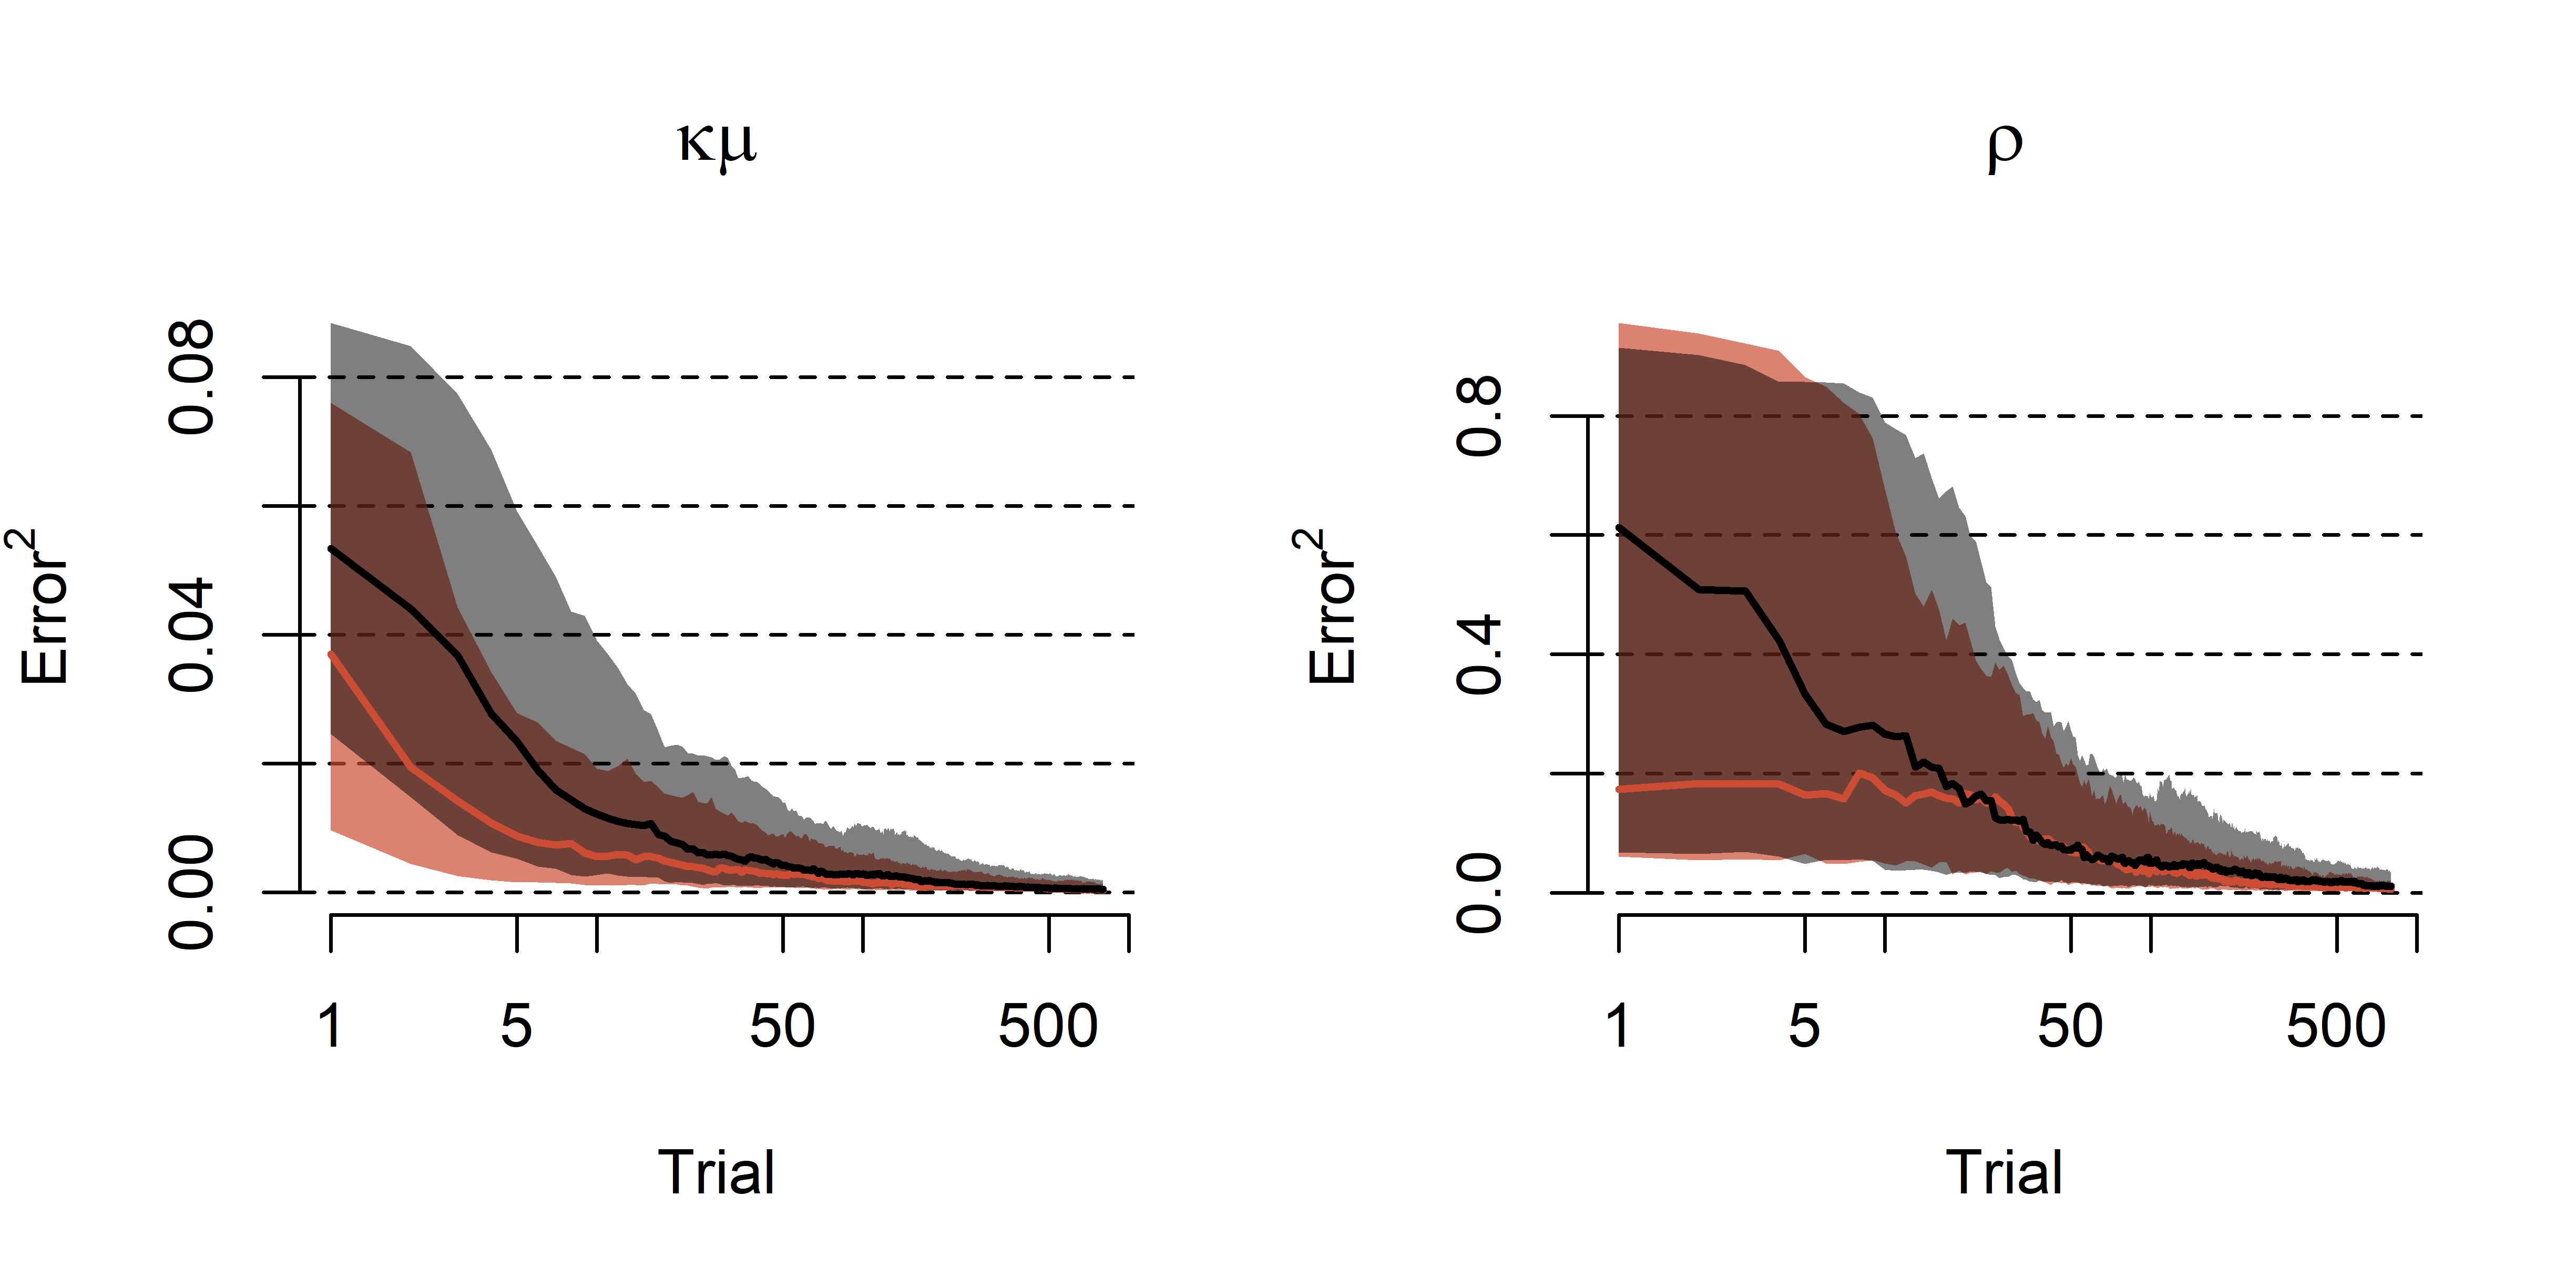
\includegraphics[scale=0.75, angle = 0]{simulation_YN_interaction_sq_error}
\caption{Procedure: Yes/No; interaction parameters. Trial-by-trial squared error between marginal means of the posterior distribution and generating parameters. Red: adaptive algorithm; black: random stimuli.}
\label{fig:simulation_YN_interaction_sq_error}
\end{figure}

\begin{figure}[H]
\centering
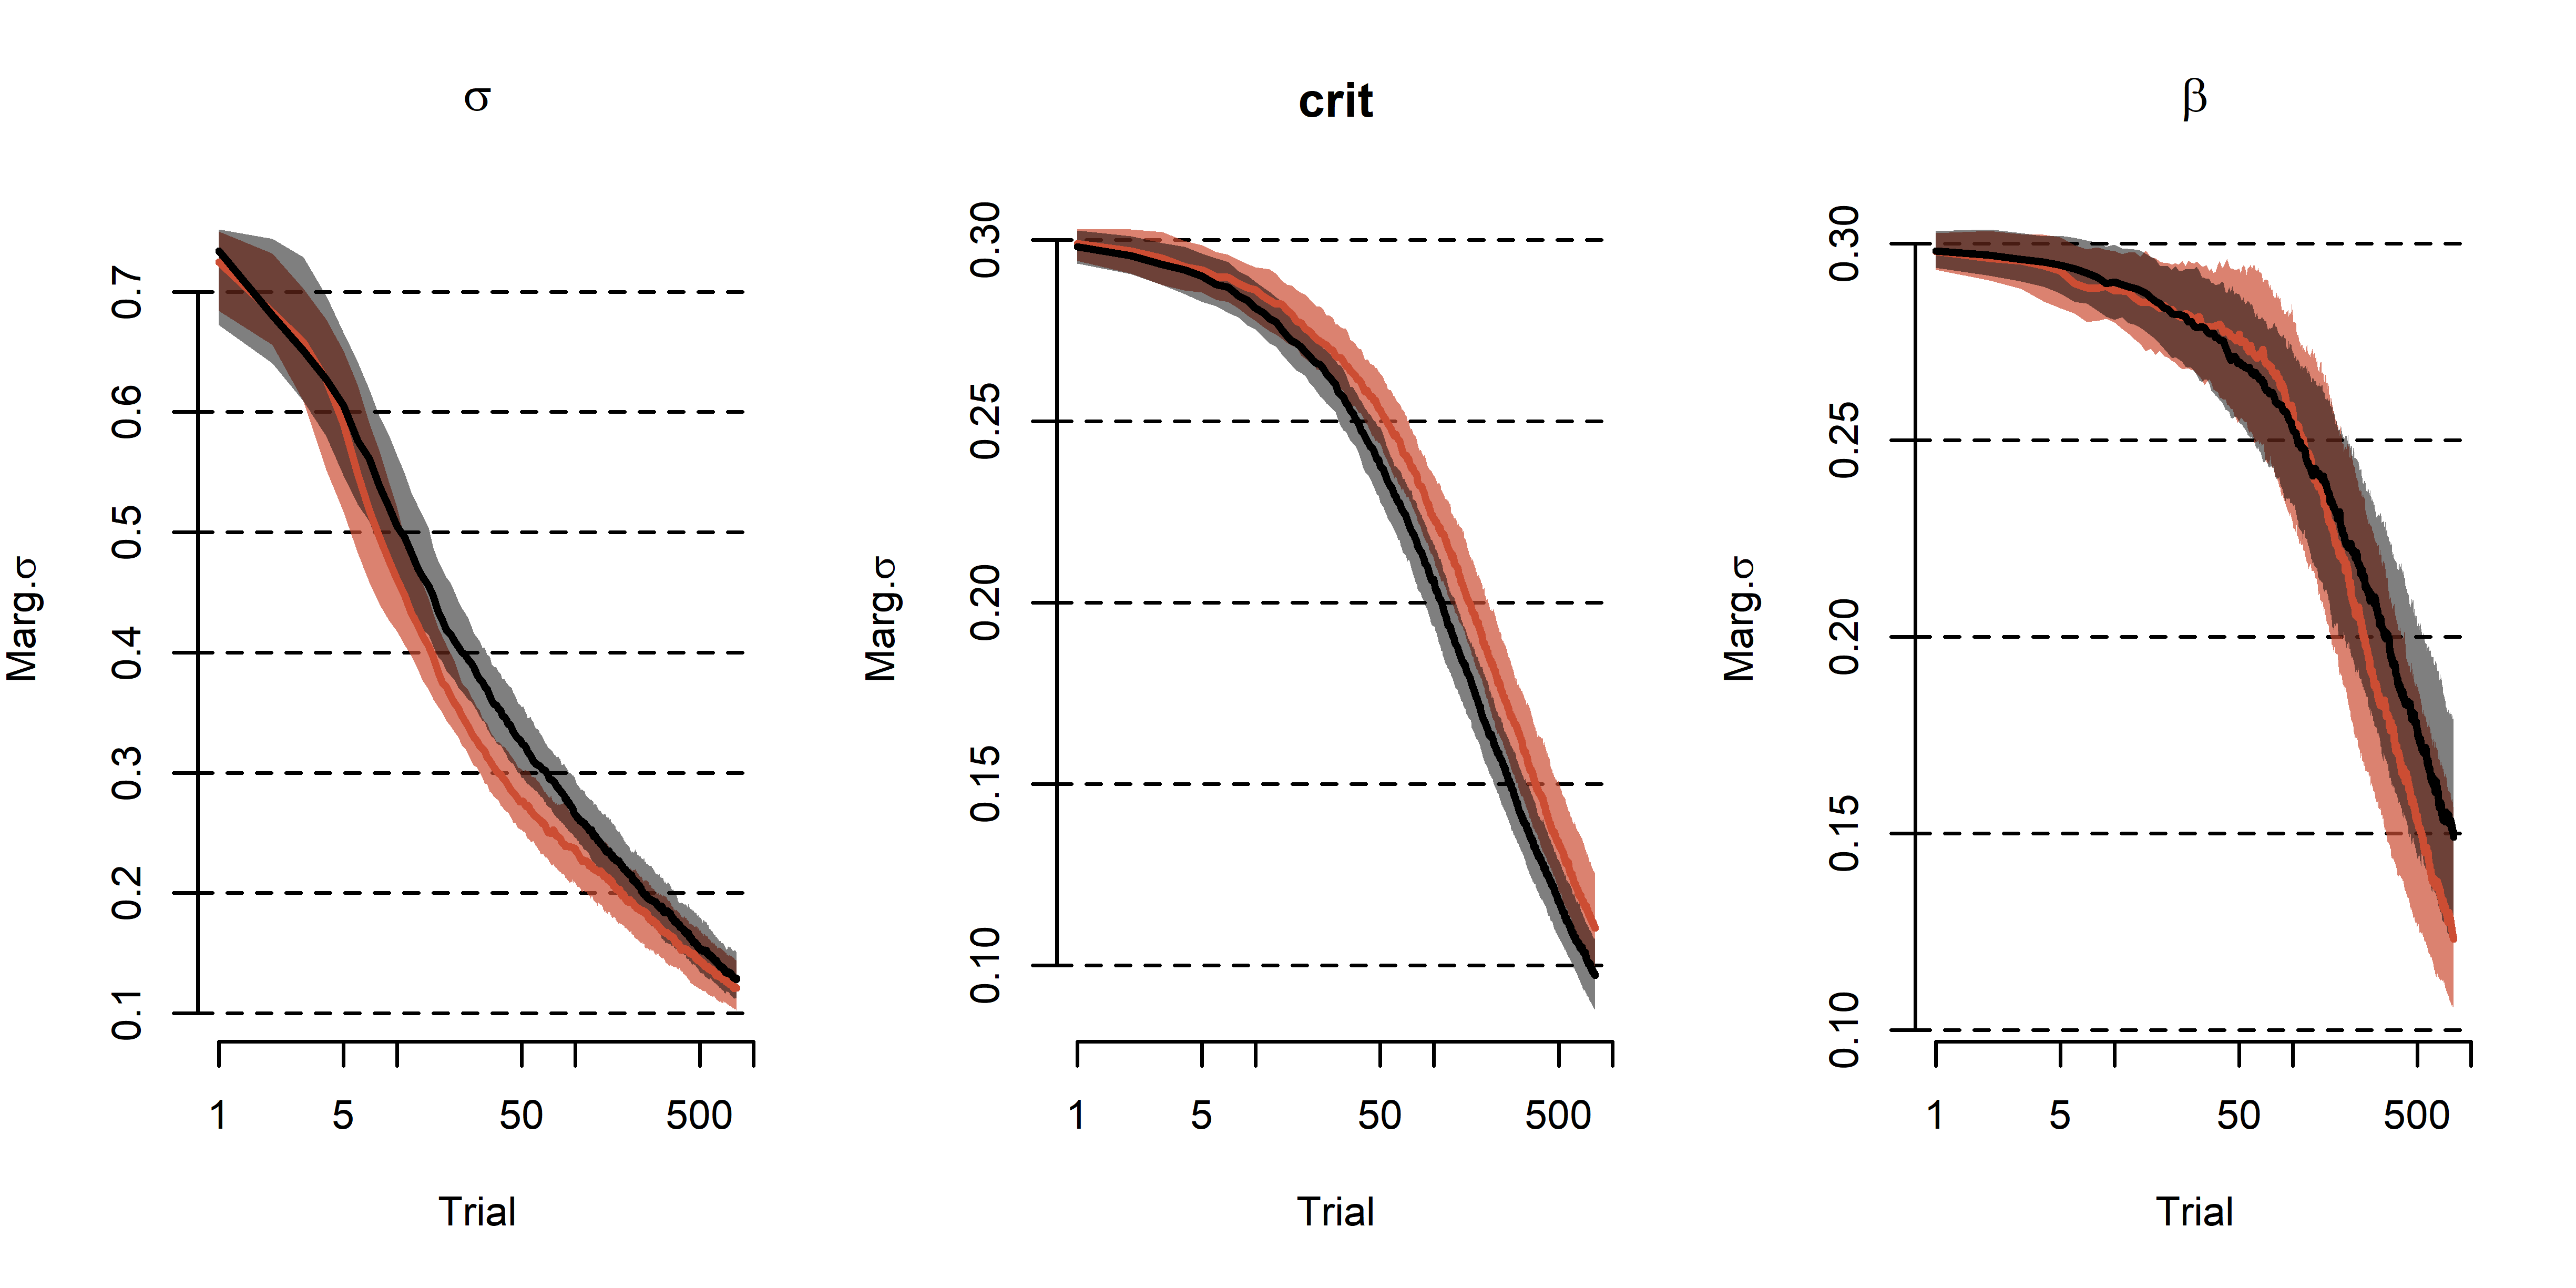
\includegraphics[scale=0.75, angle = 0]{simulation_YN_sensory_SD}
\caption{Procedure: Yes/No; sensory parameters. Trial-by-trial marginal standard deviations. Red: adaptive algorithm; black: random stimuli.}
\label{fig:simulation_YN_sensory_SD}
\end{figure}

\begin{figure}[H]
\centering
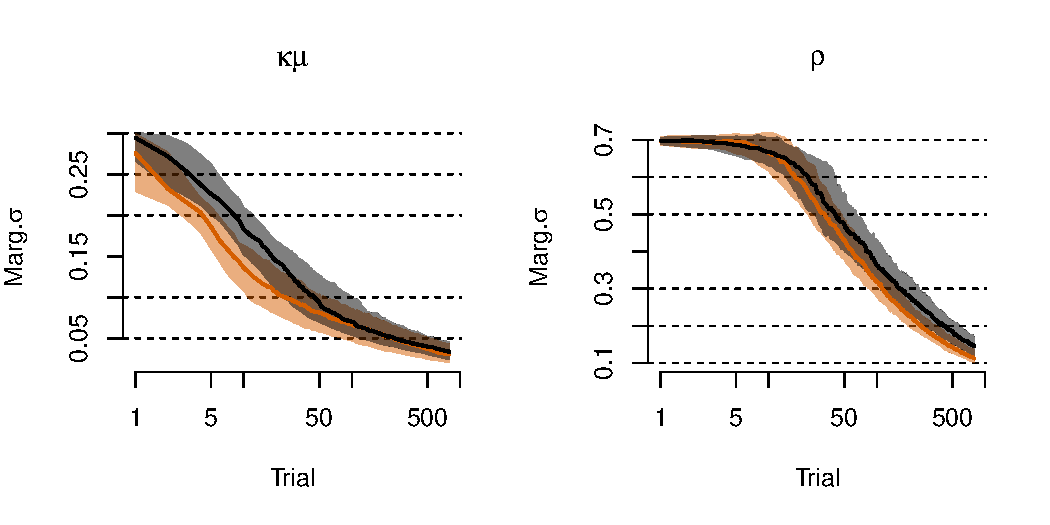
\includegraphics[scale=0.75, angle = 0]{simulation_YN_interaction_SD}
\caption{Procedure: Yes/No; interaction parameters. Trial-by-trial marginal standard deviations. Red: adaptive algorithm; black: random stimuli.}
\label{fig:simulation_YN_interaction_SD}
\end{figure}

\begin{figure}[H]
\centering
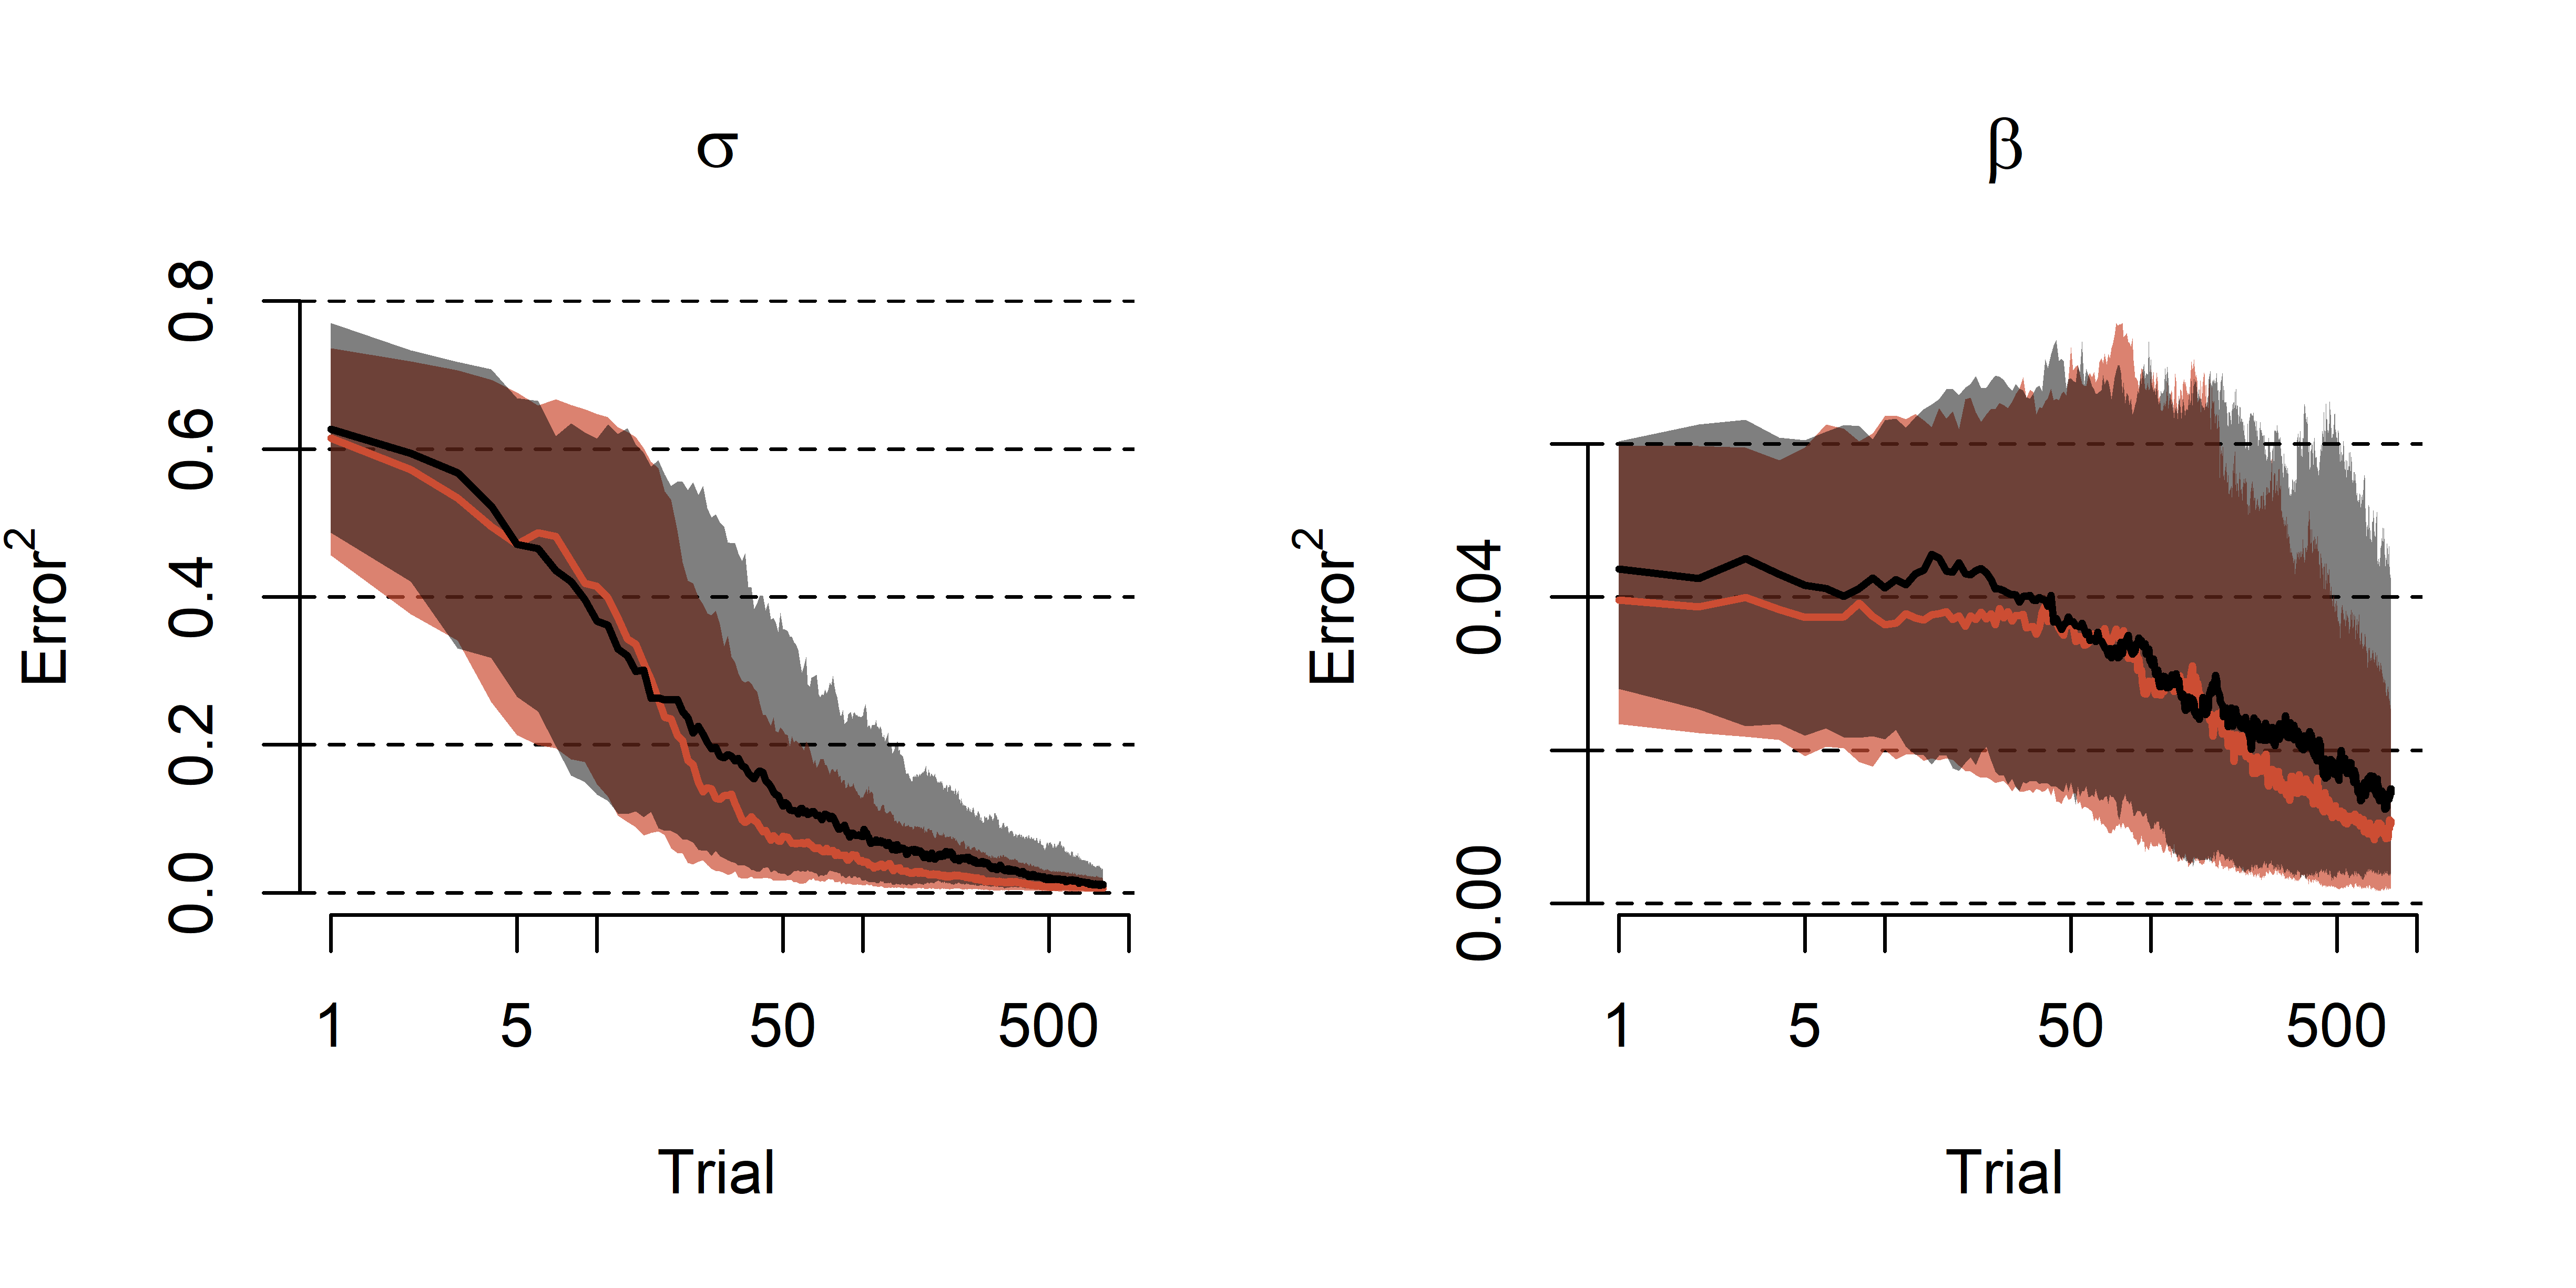
\includegraphics[scale=0.75, angle = 0]{simulation_AFC_sensory_sq_error}
\caption{Procedure: 2I-4AFC; sensory parameters. Trial-by-trial squared error between marginal means of the posterior distribution and generating parameters. Red: adaptive algorithm; black: random stimuli.}
\label{fig:simulation_AFC_sensory_sq_error}
\end{figure}

\begin{figure}[H]
\centering
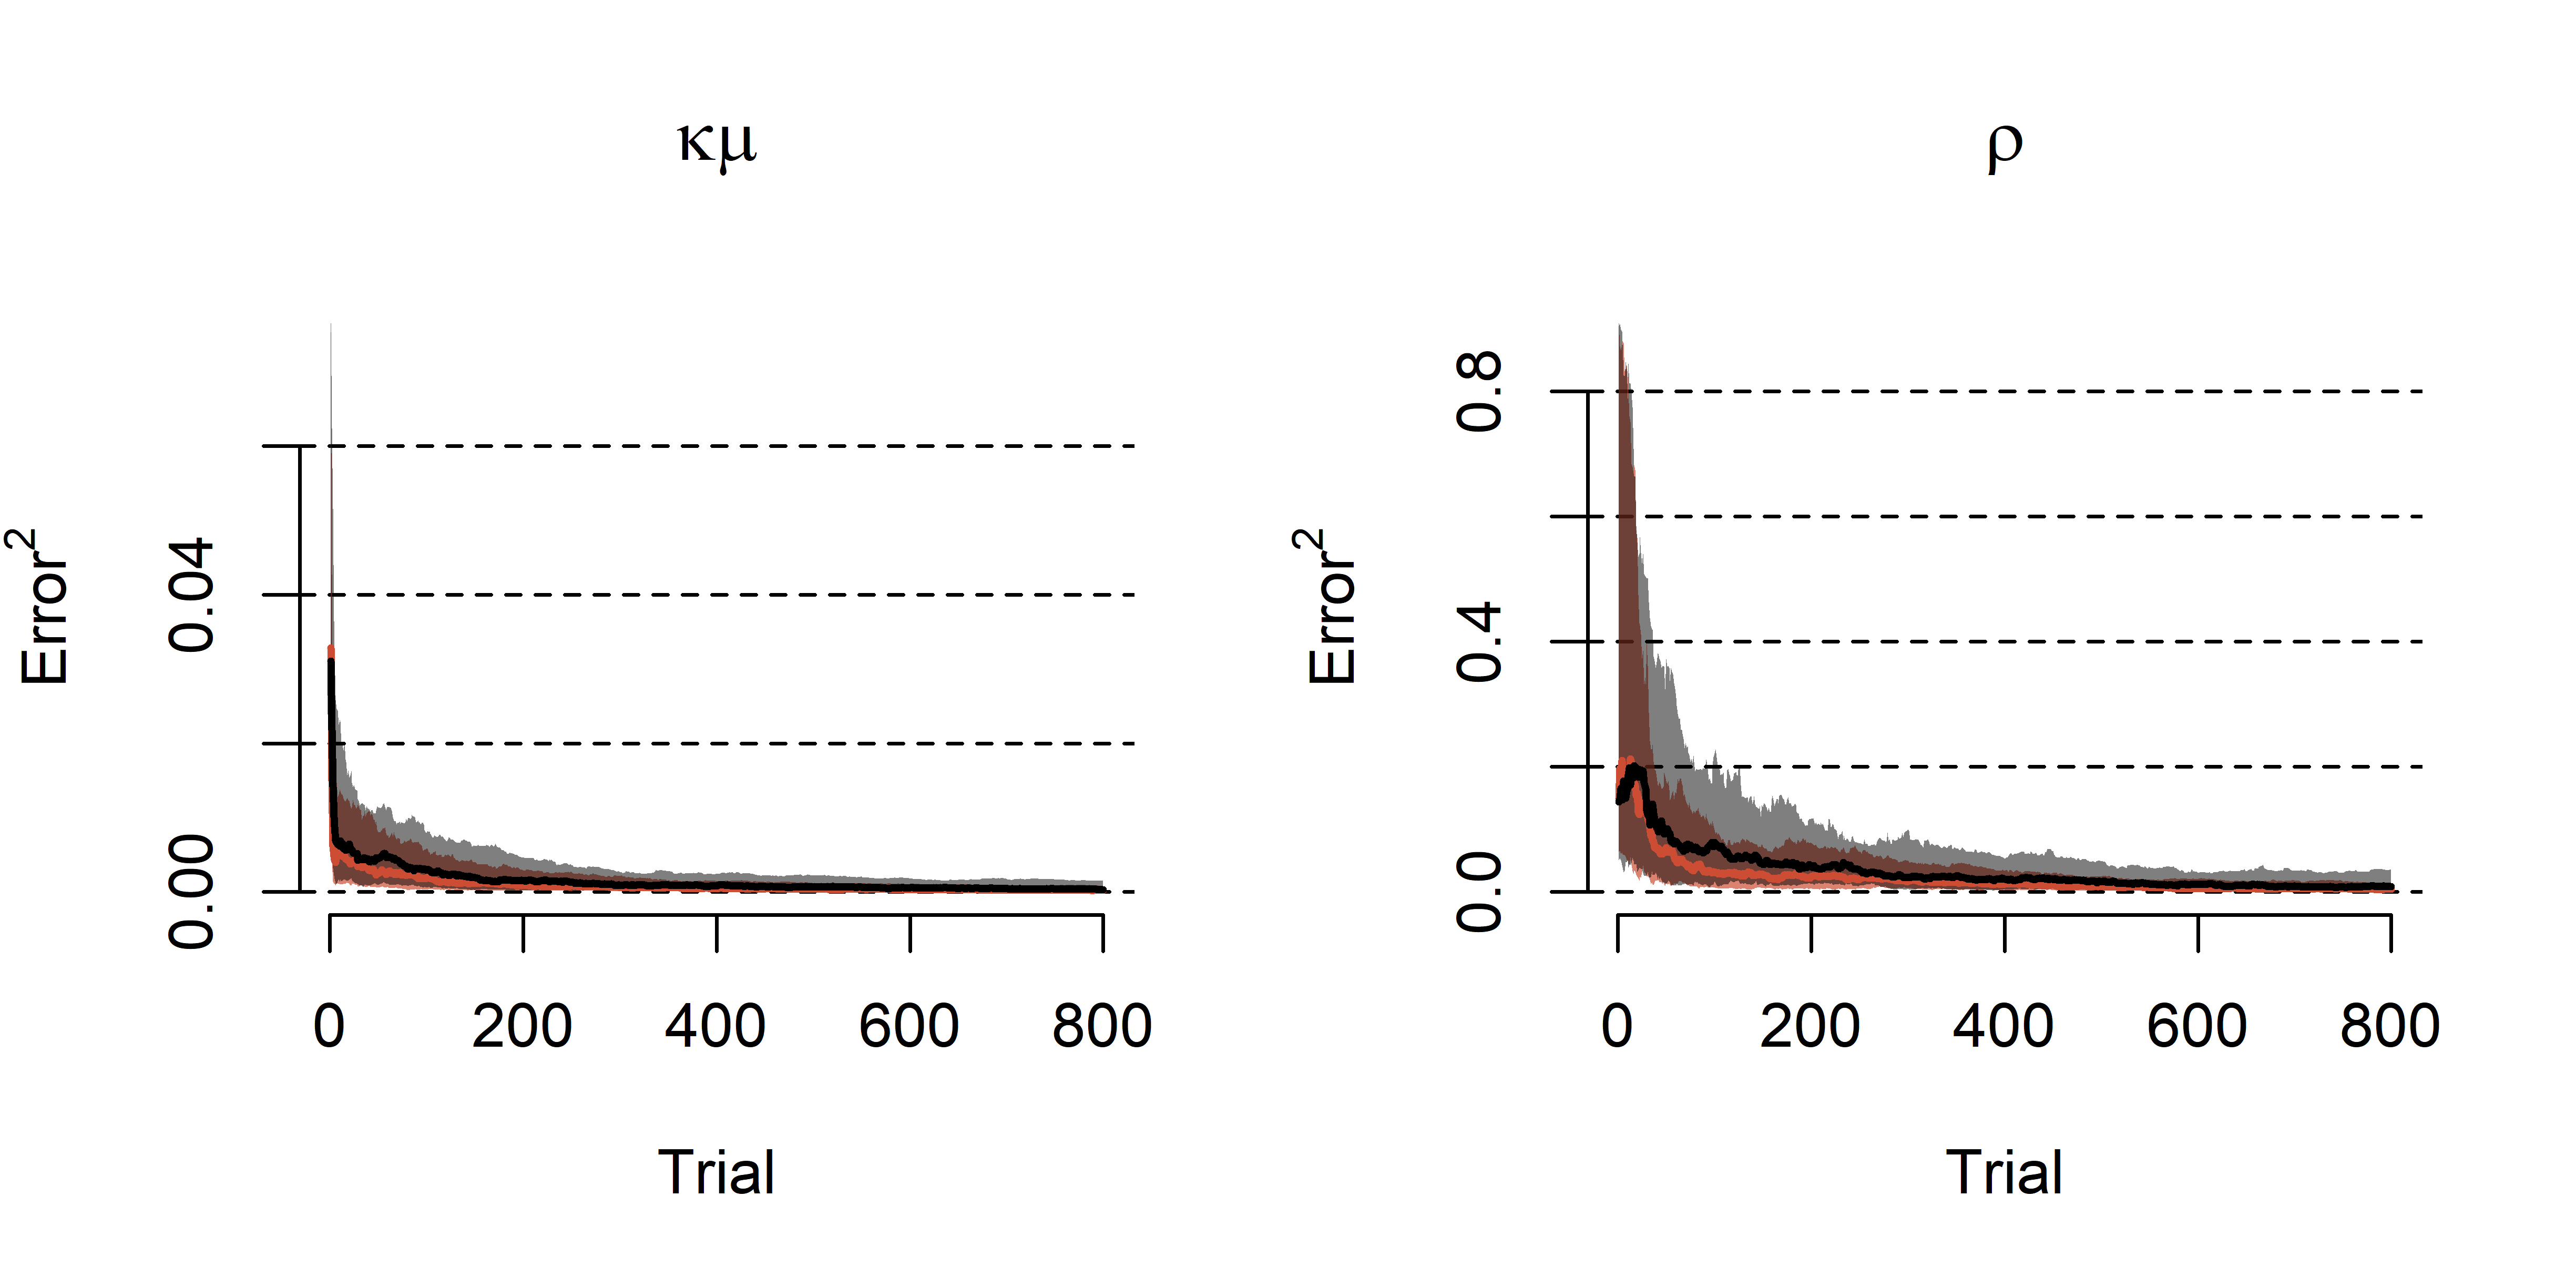
\includegraphics[scale=0.75, angle = 0]{simulation_AFC_interaction_sq_error}
\caption{Procedure: 2I-4AFC; interaction parameters. Trial-by-trial squared error between marginal means of the posterior distribution and generating parameters. Red: adaptive algorithm; black: random stimuli.}
\label{fig:simulation_AFC_interaction_sq_error}
\end{figure}

\begin{figure}[H]
\centering
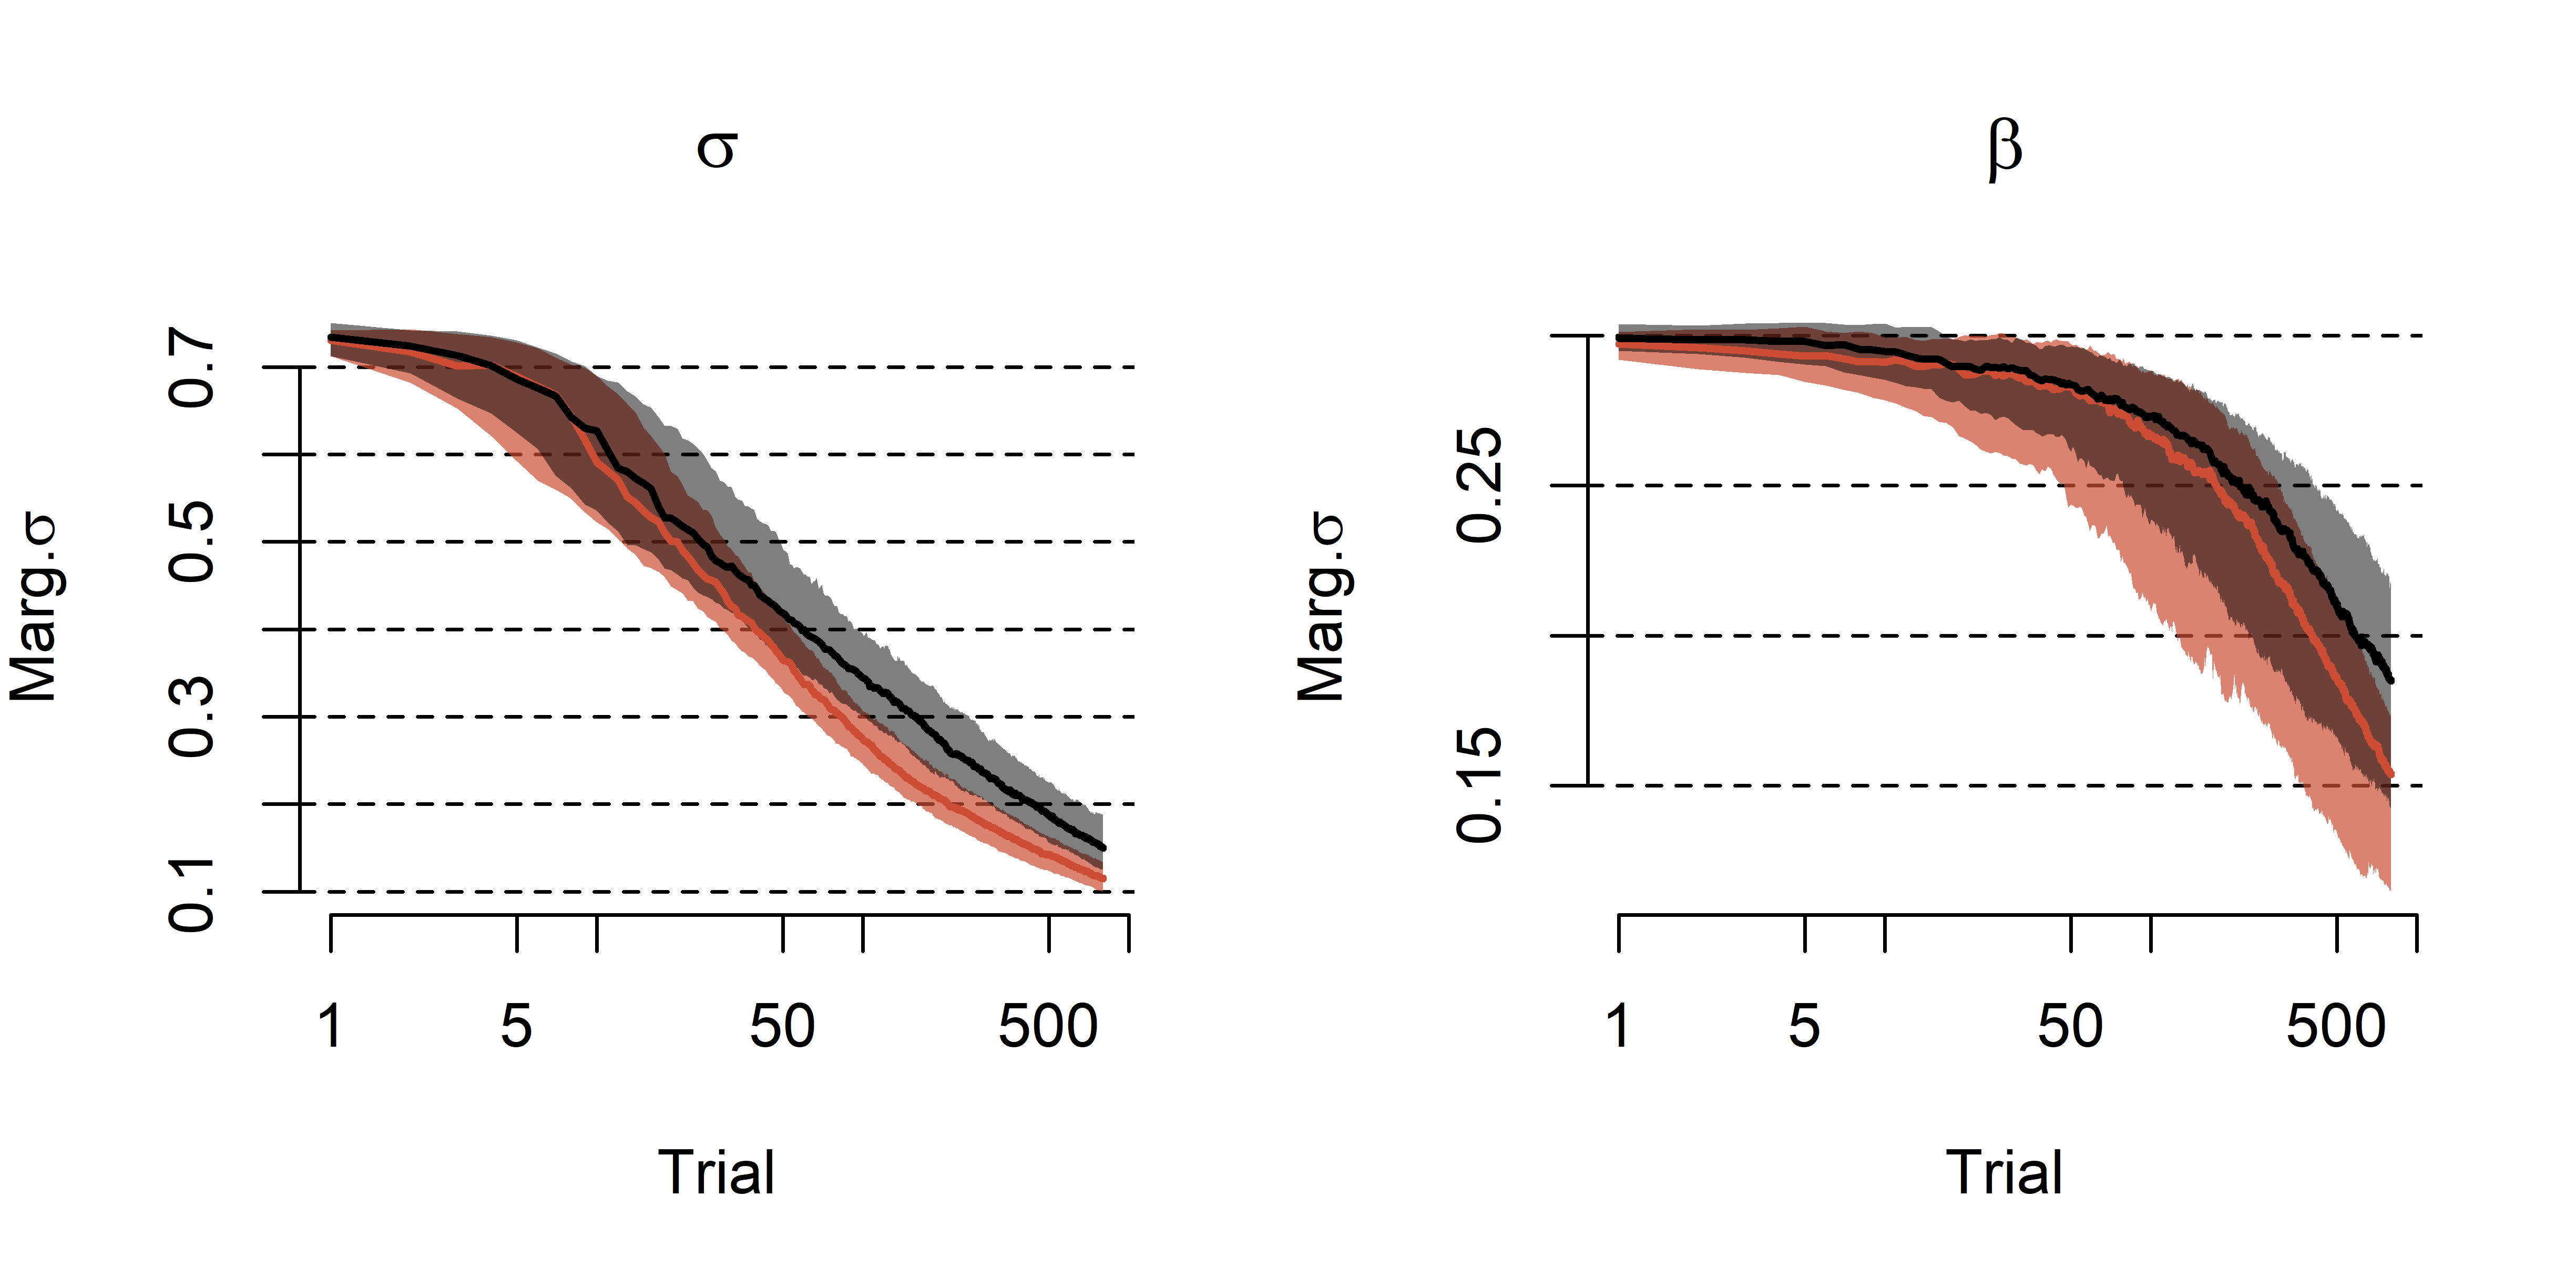
\includegraphics[scale=0.75, angle = 0]{simulation_AFC_sensory_SD}
\caption{Procedure: 2I-4AFC; sensory parameters. Trial-by-trial marginal standard deviations. Red: adaptive algorithm; black: random stimuli.}
\label{fig:simulation_AFC_sensory_SD}
\end{figure}

\begin{figure}[H]
\centering
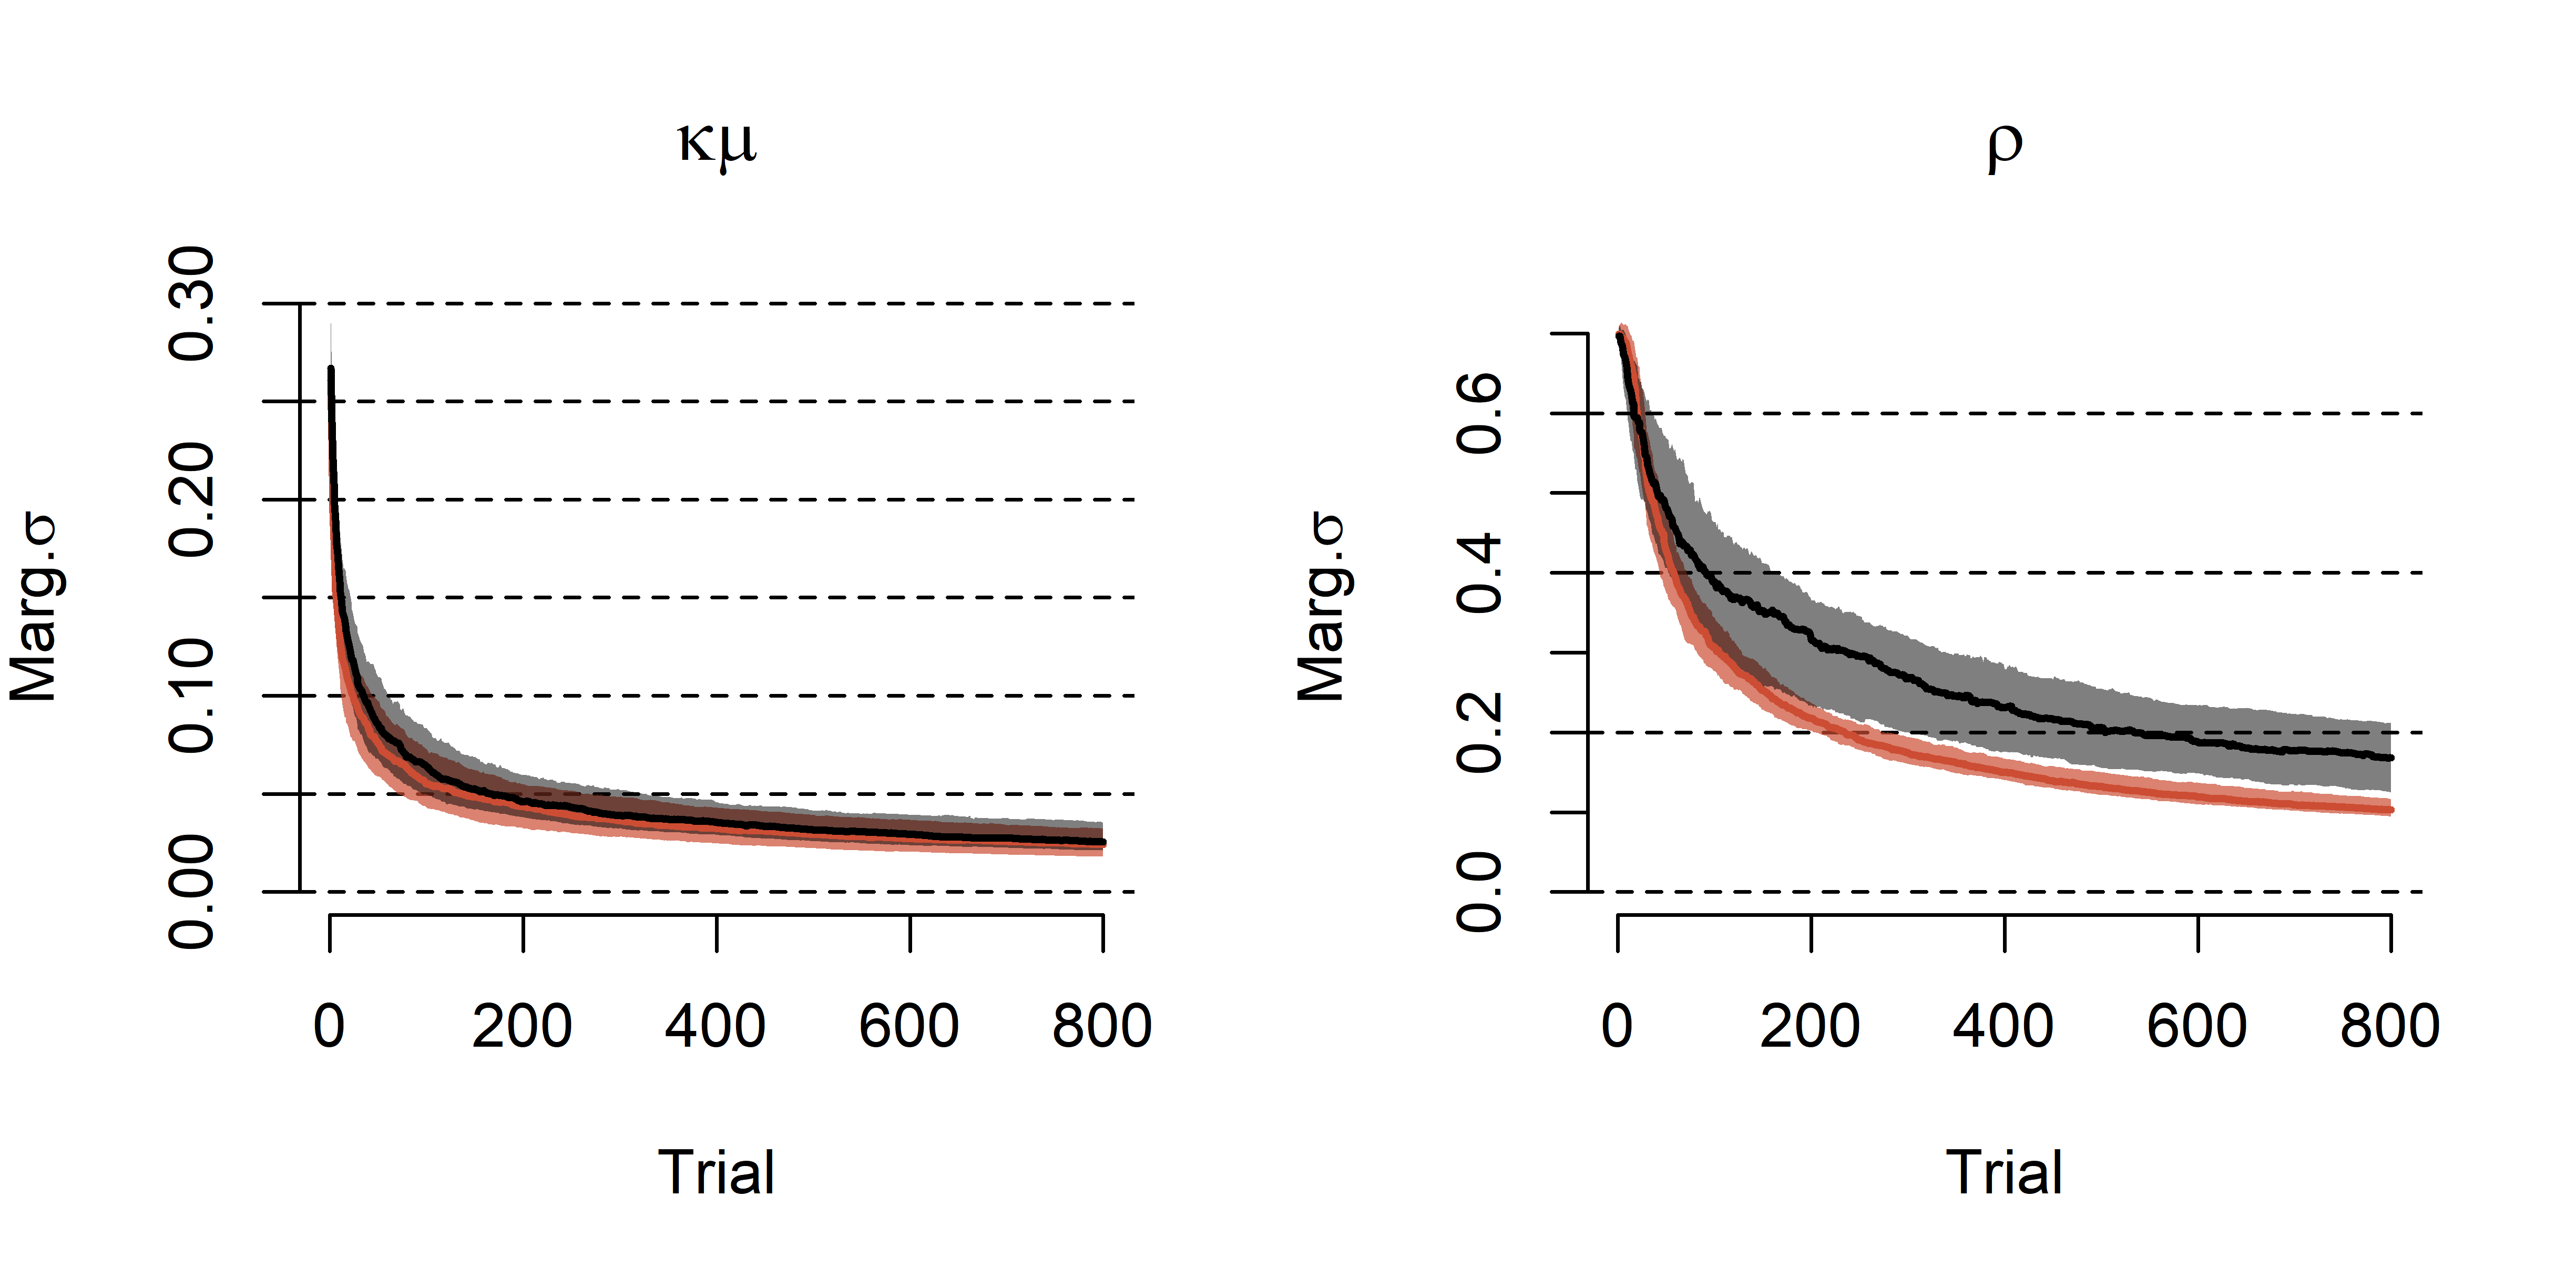
\includegraphics[scale=0.75, angle = 0]{simulation_AFC_interaction_SD}
\caption{Procedure: 2I-4AFC; interaction parameters. Trial-by-trial marginal standard deviations. Red: adaptive algorithm; black: random stimuli.}
\label{fig:simulation_AFC_interaction_SD}
\end{figure}

\paragraph{Hierarchical model}

A hierarchical model was fit to both the marginal standard deviations and squared errors at the last trial to get a more quantitative understanding of the differences at that point. This should be considered as a first-order approximation of a more complete model of performance. Why only the estimates at the last trial are presented is because for any simple model which breaks the performance down in two factors, namely the final values and the speed at which they were arrived at, only one of the factors needs to be known. This is because all of the algorithms start from the same values (the prior distribution) and are run for the same amount of time (800 trials). Of course some more sophisticated model, that would perform more complex decomposition of performance could be used, but the development of such algorithm is beyond the scope of this thesis. 

A common dummy coded linear model with Gaussian errors was used. The slopes, intercepts and standard deviations were pooled inside each condition, which means that e.g. all of the marginal standard deviations in the Yes/No condition with adaptively selected stimuli were given a common hyperprior. The models were fit using Stan.

Data was standardized before fitting ($y' = (y - \overline{y}) / \text{SD}(y) $). Parameter-specific $\beta'$ coefficients (slopes fit to standardized data) of the linear model are shown in Figures from \ref{fig:qs_YN_SD} to \ref{fig:qs_AFC_sq_error}. In all plots the thicker parts indicate 50\% and narrower lines 95\% equal-tailed intervals\footnote{\textit{Equal-tailed interval} (ETI) means the interval between some percentiles of the posterior distribution \citep[p. 342]{kruschke2015}, here for example the interval between 2.5\% and 97.5\% for the 95\% ETI.}. Positive values indicate better performance by the adaptive algorithm.

\begin{figure}[H]
\centering
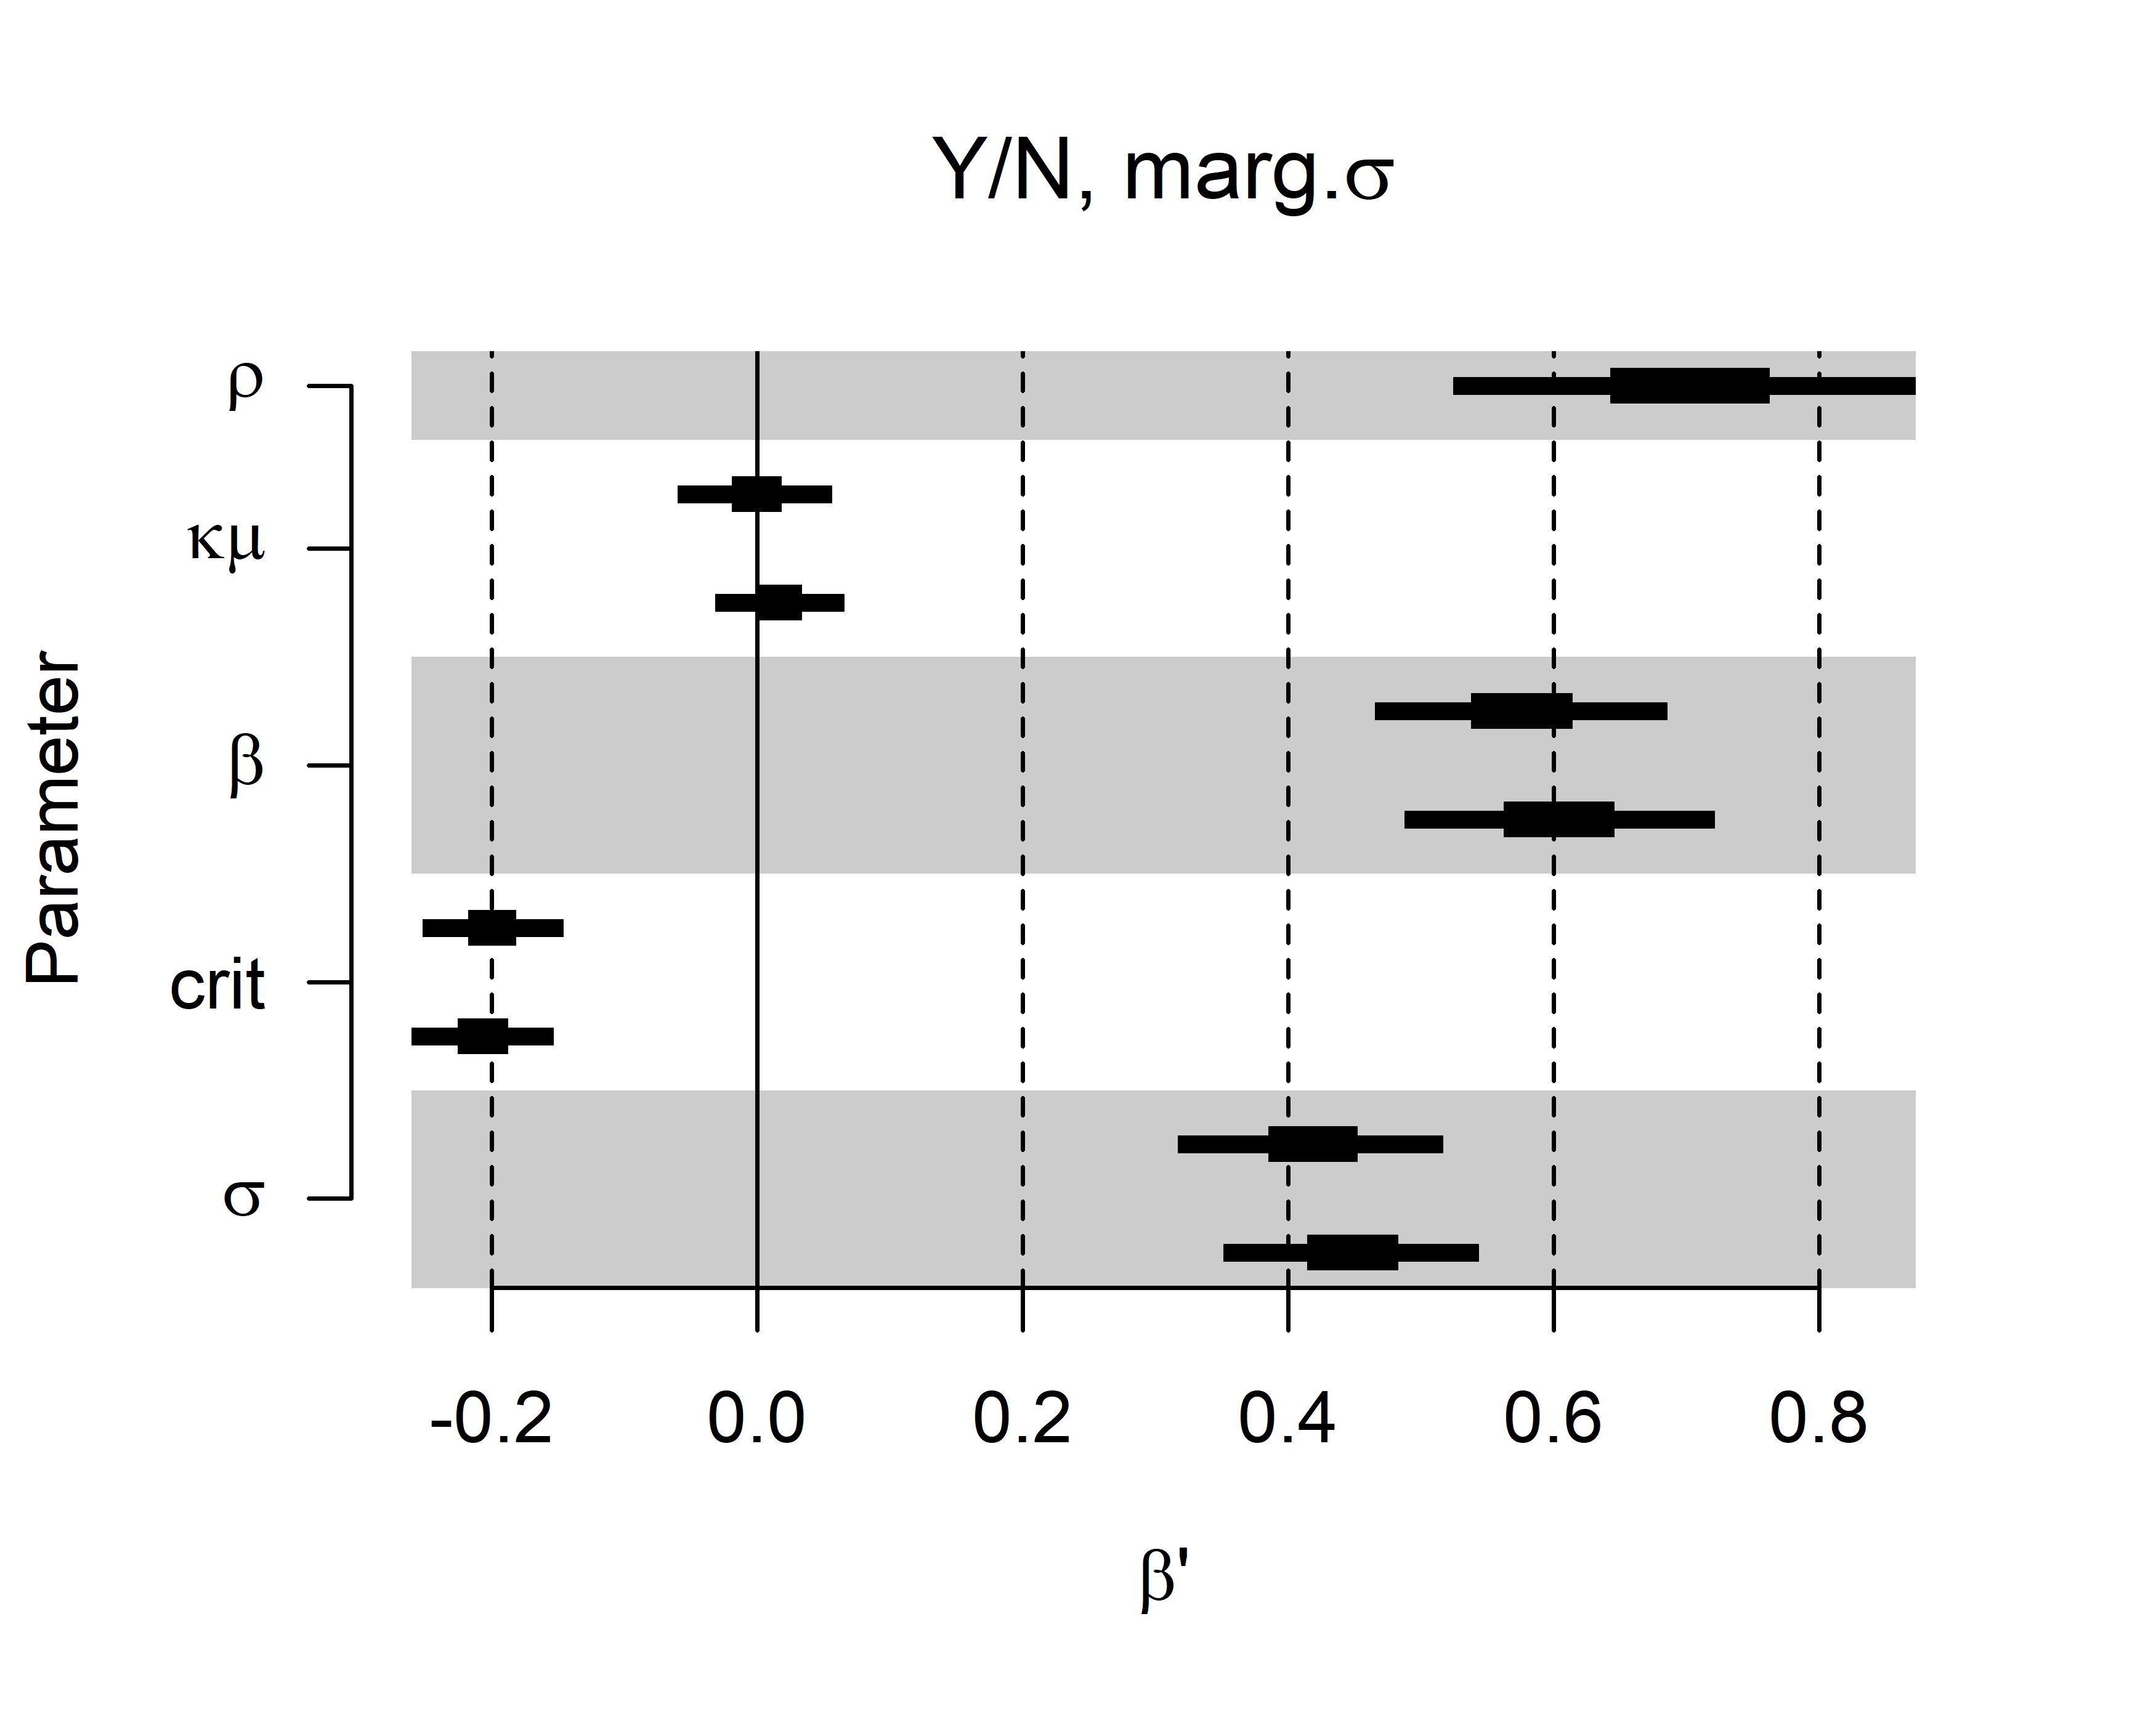
\includegraphics[scale=0.75]{qs_YN_SD}
\caption{Procedure: Yes/No. $\beta'$ coefficients for the difference between adaptive and random algorithms in marginal standard deviations.}
\label{fig:qs_YN_SD}
\end{figure} 

\begin{figure}[H]
\centering
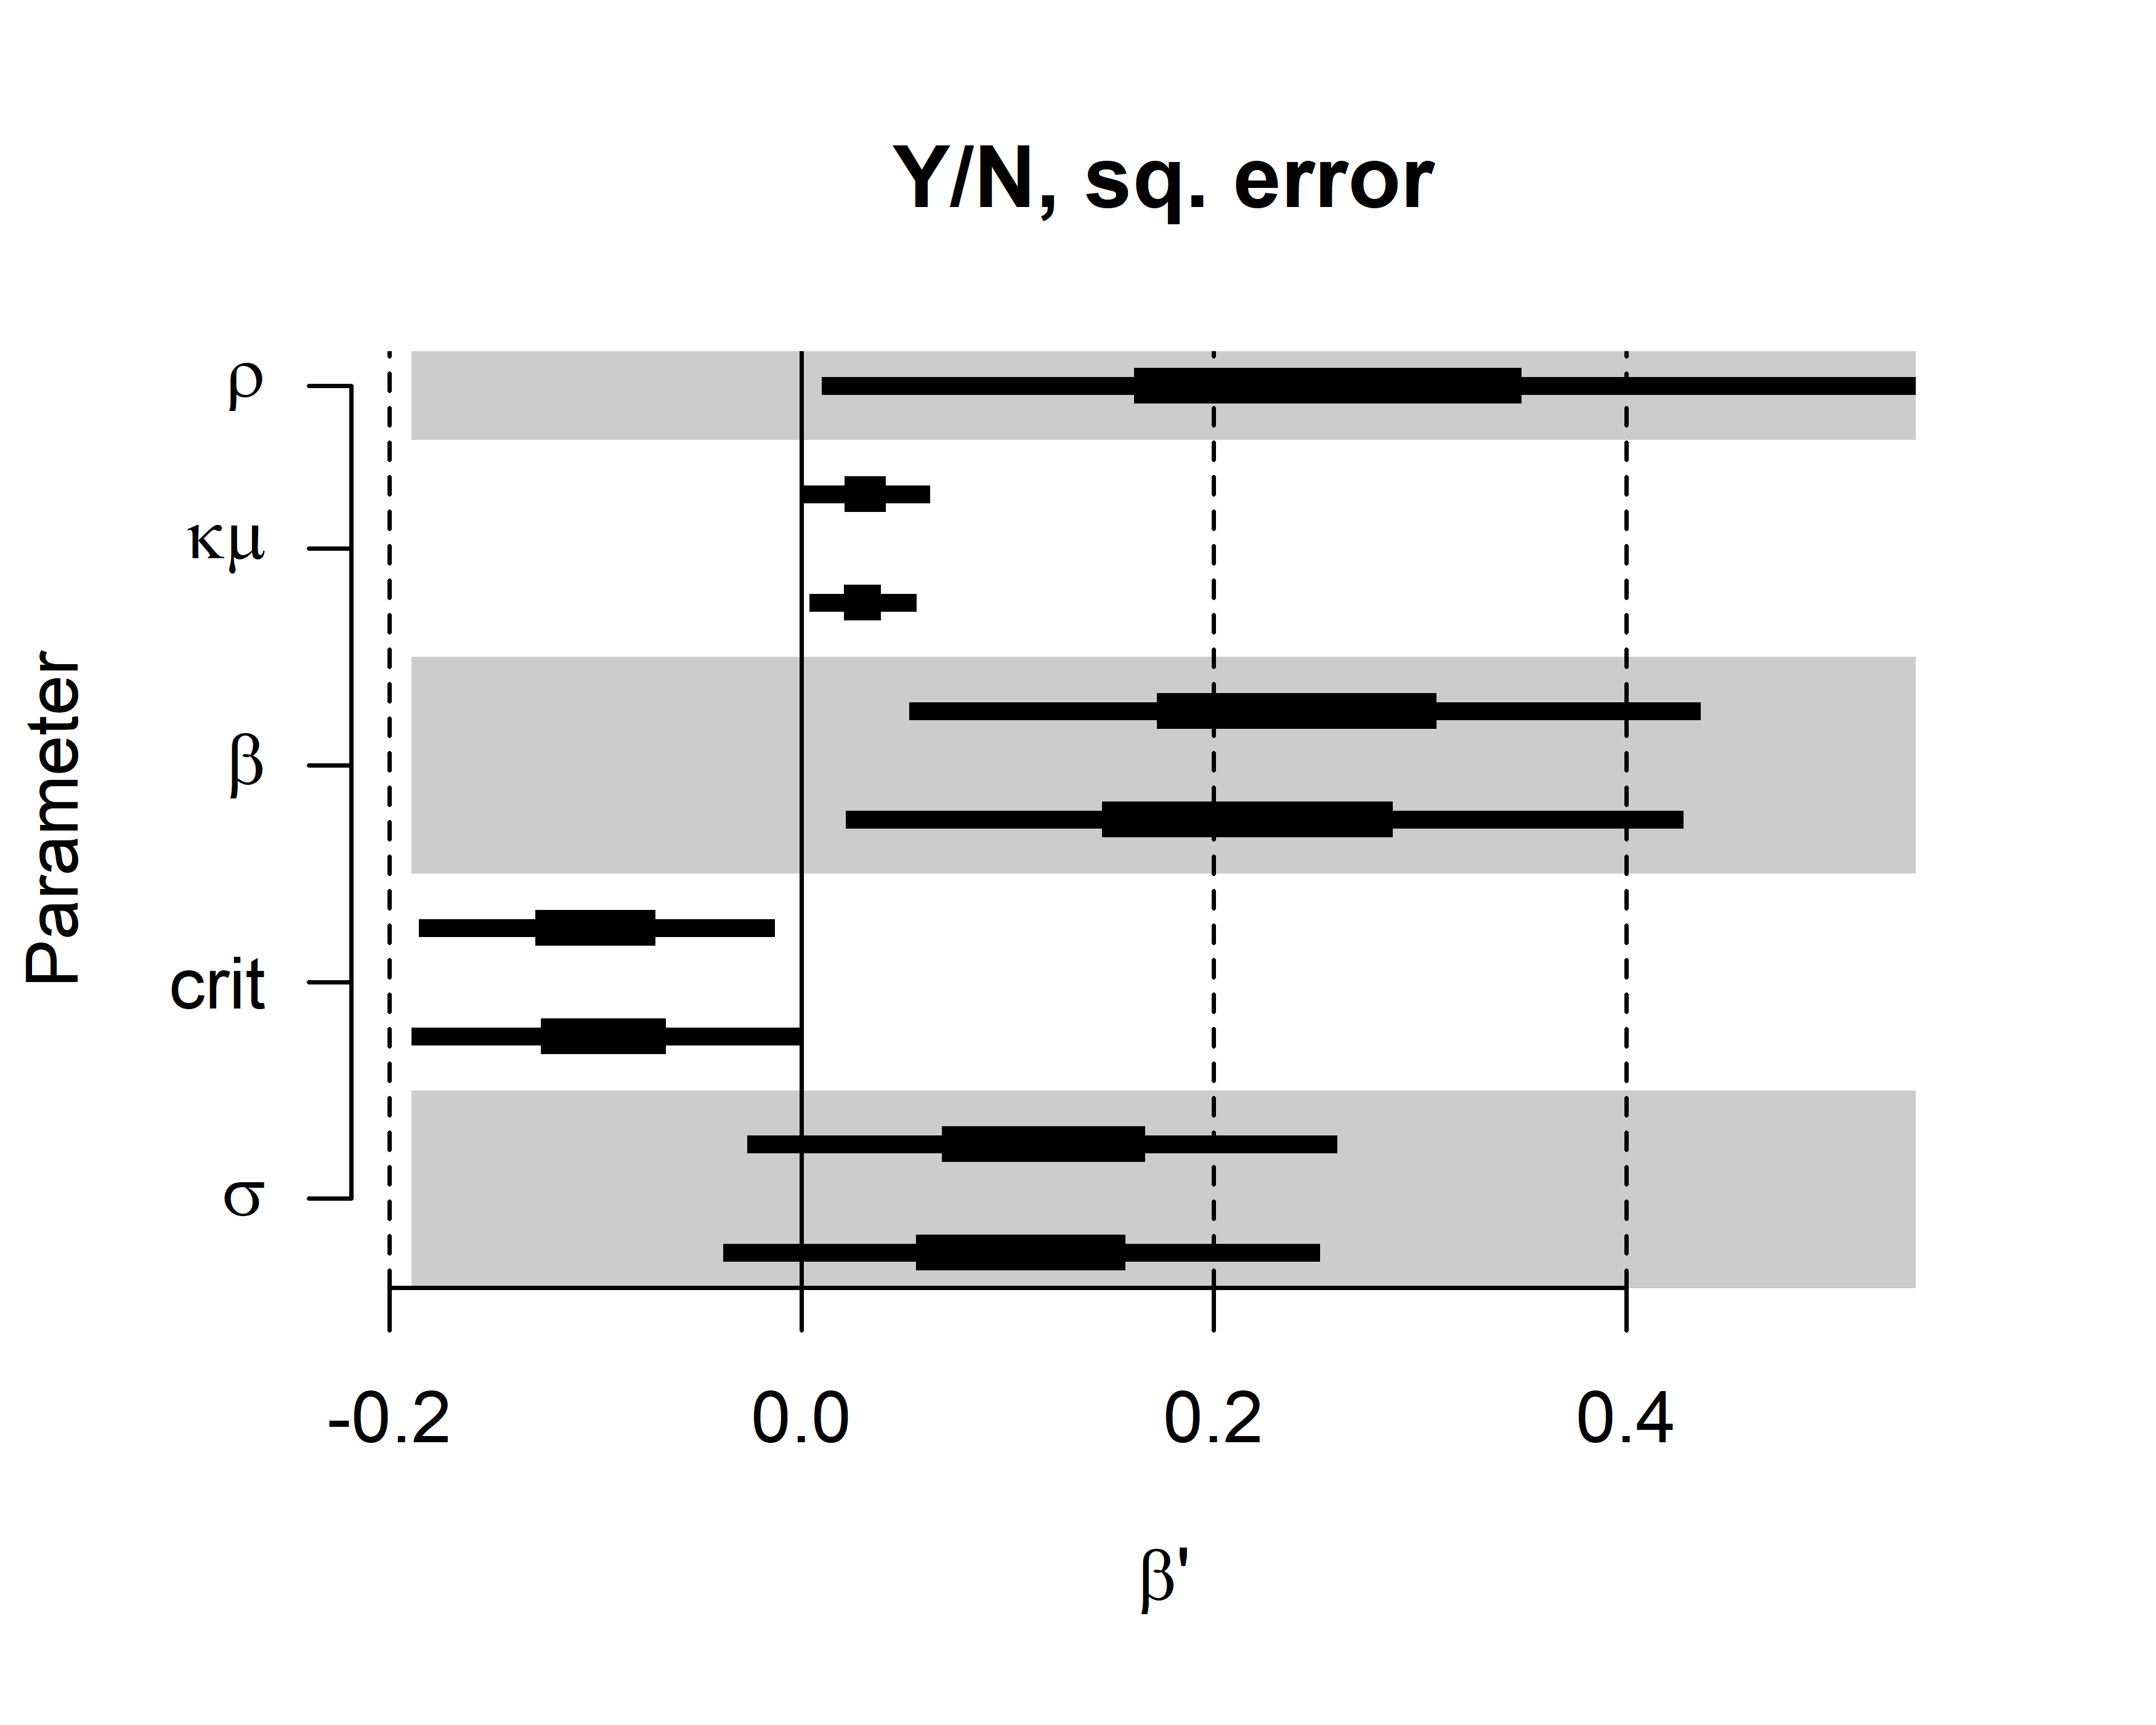
\includegraphics[scale=0.75]{qs_YN_sq_error}
\caption{Procedure: Yes/No. $\beta'$ coefficients for the difference between adaptive and random algorithms in squared errors between marginal means and generating parameters.}
\label{fig:qs_YN_sq_error}
\end{figure} 

\begin{figure}[H]
\centering
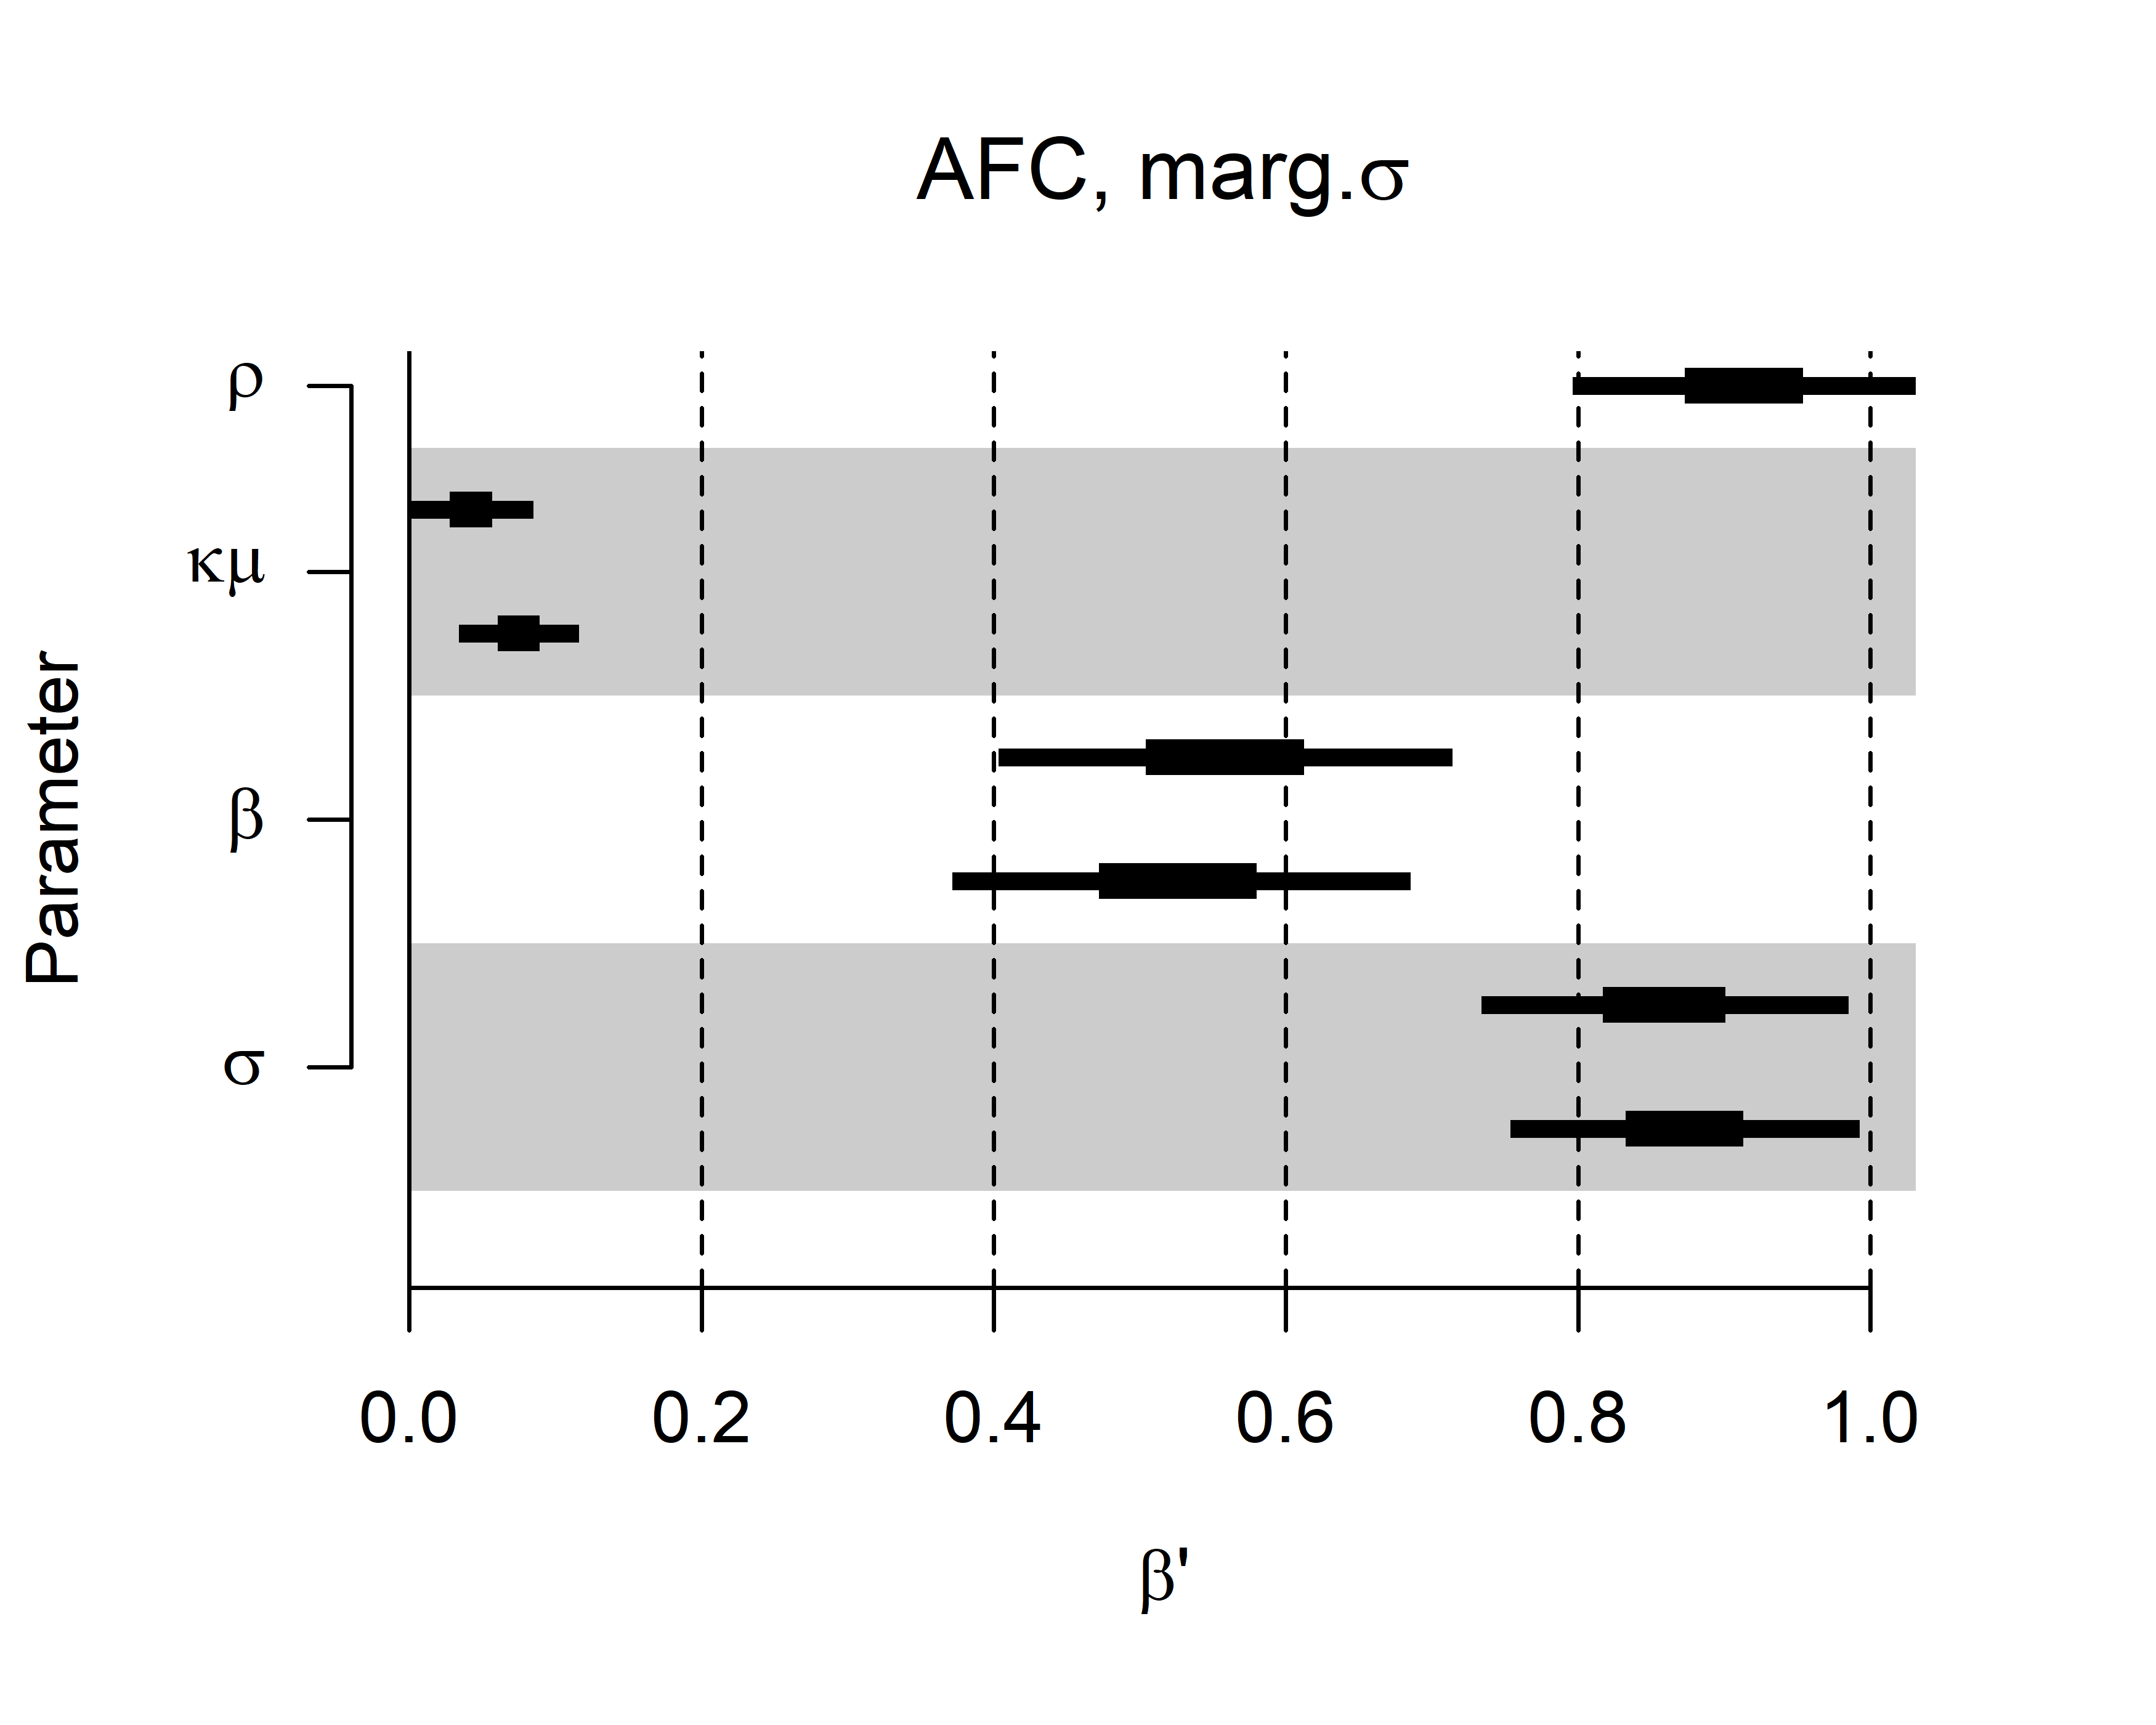
\includegraphics[scale=0.75]{qs_AFC_SD}
\caption{Procedure: 2I-4AFC. $\beta'$ coefficients for the difference between adaptive and random algorithms in marginal standard deviations.}
\label{fig:qs_AFC_SD}
\end{figure} 

\begin{figure}[H]
\centering
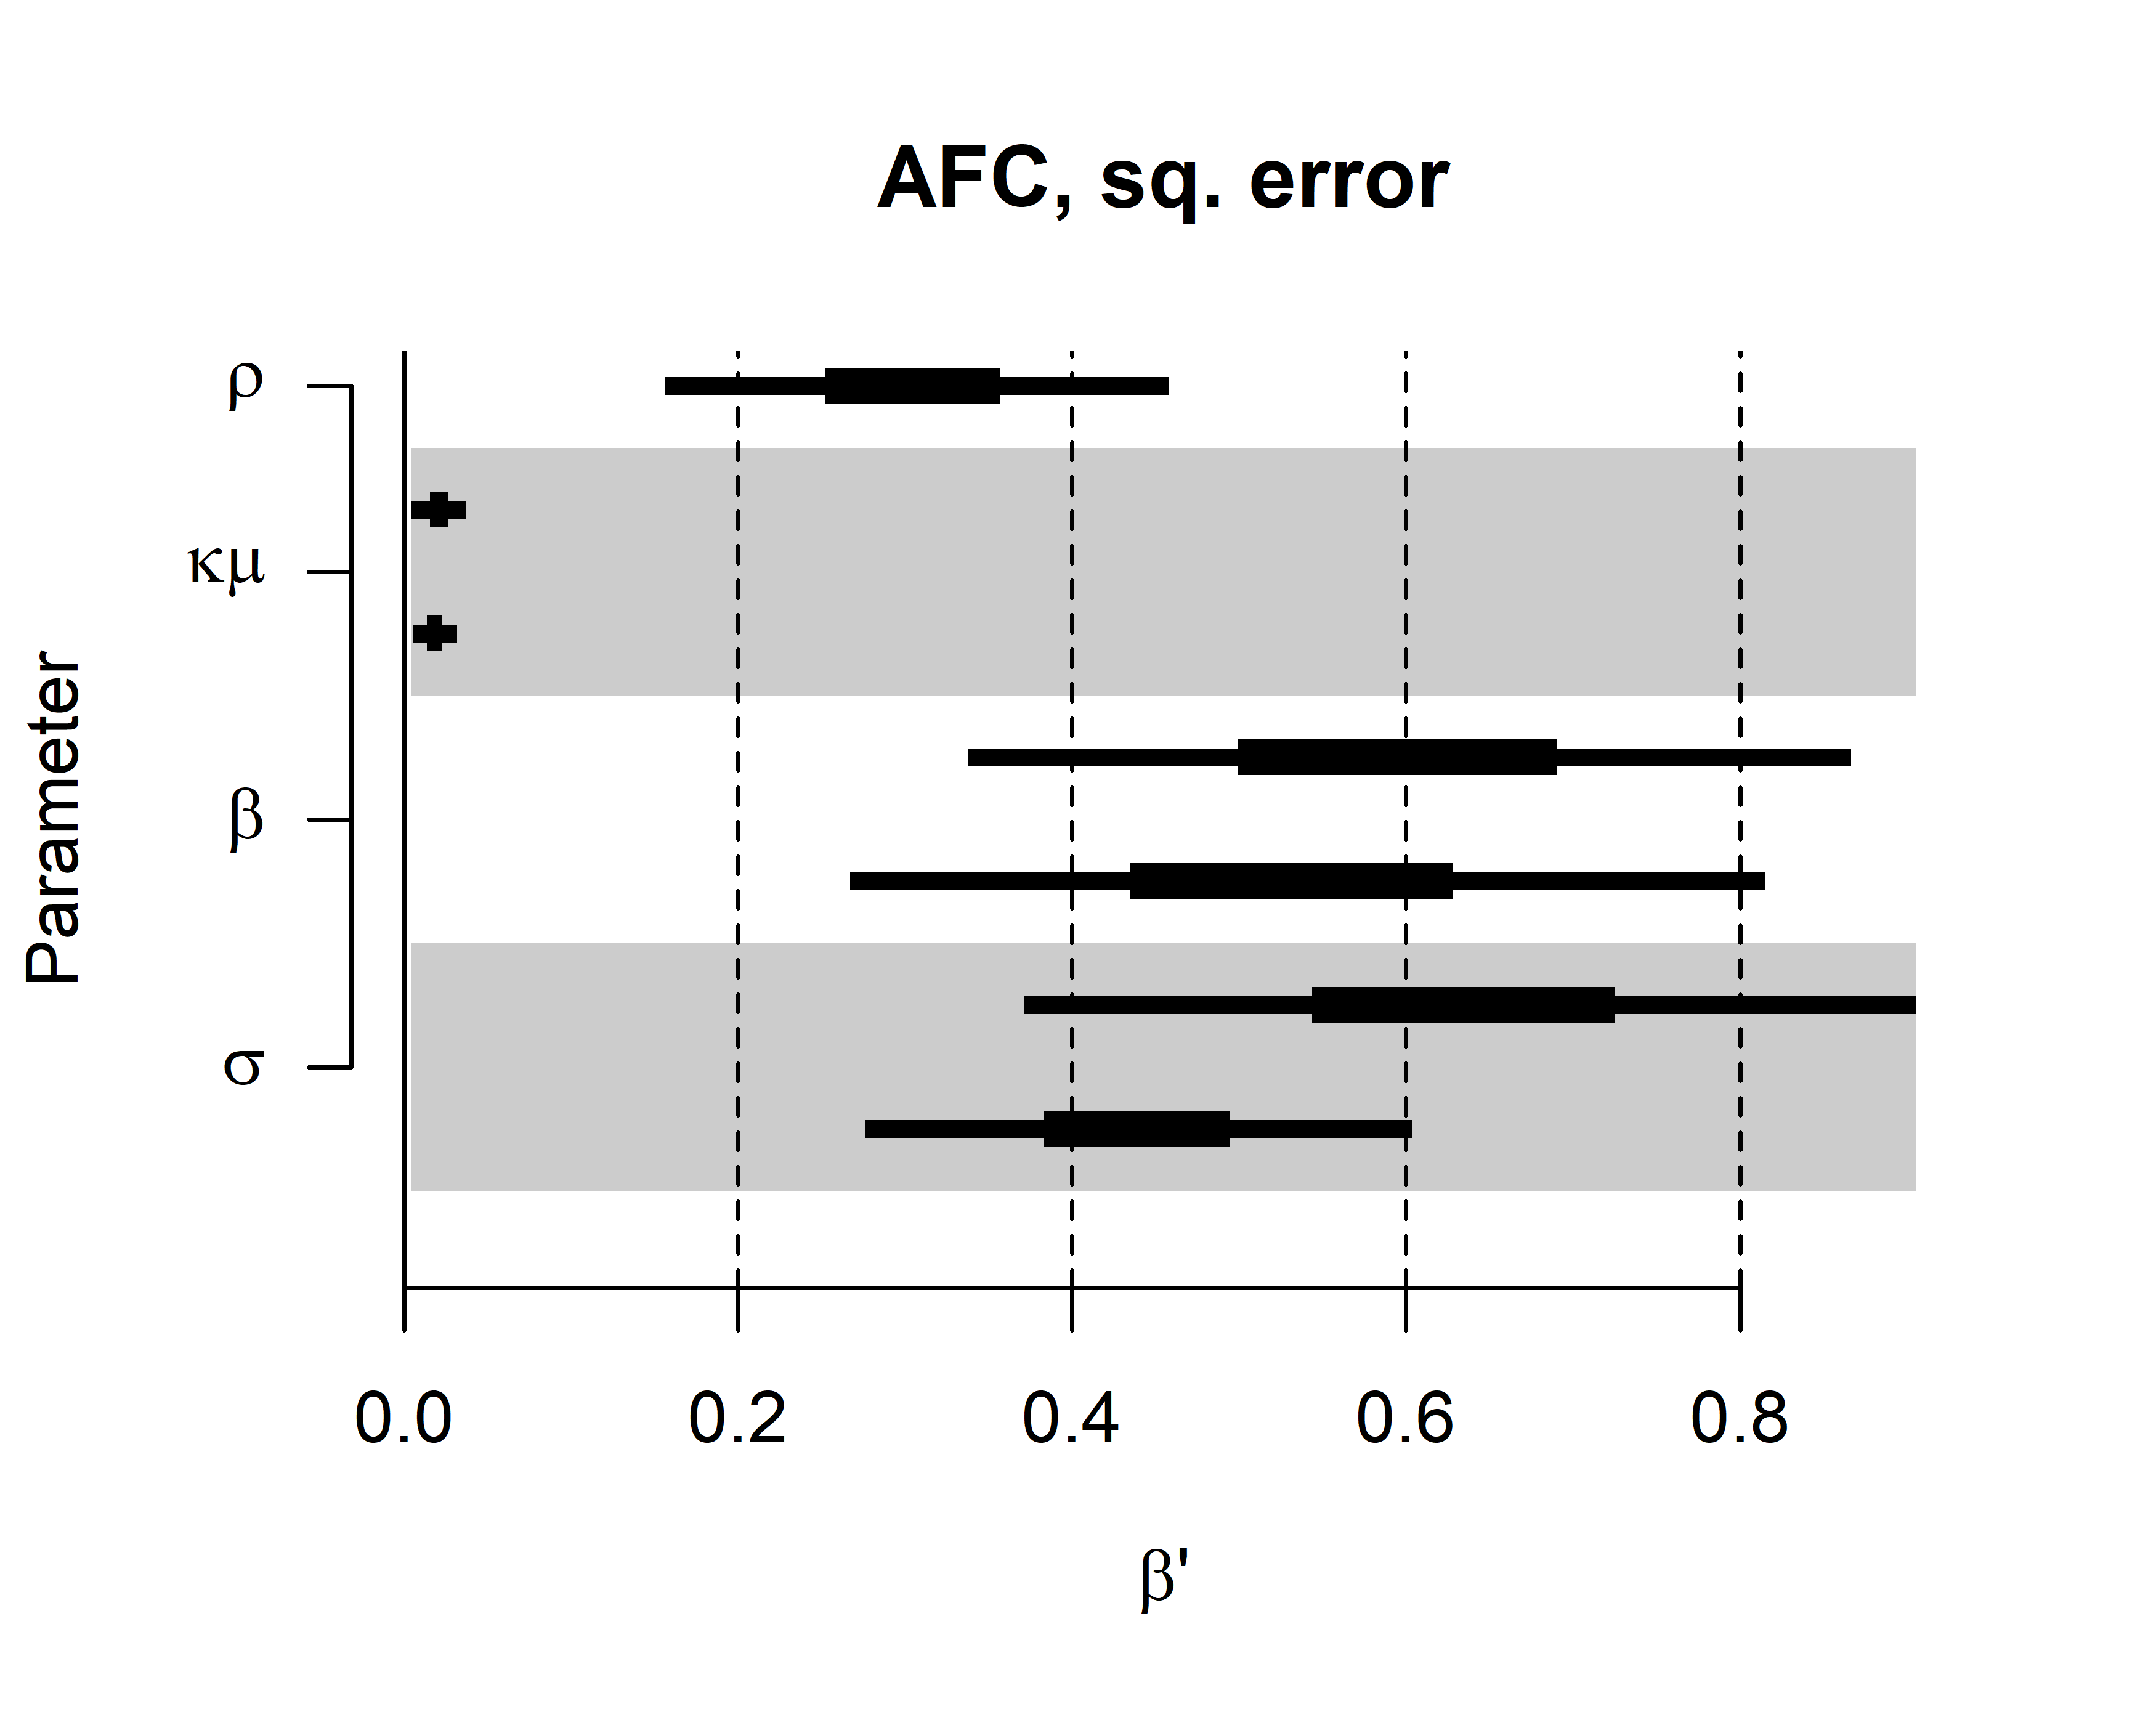
\includegraphics[scale=0.75]{qs_AFC_sq_error}
\caption{Procedure: 2I-4AFC. $\beta'$ coefficients for the difference between adaptive and random algorithms in squared errors between marginal means and generating parameters.}
\label{fig:qs_AFC_sq_error}
\end{figure} 

\subsection{Discussion}

\paragraph{Question 1: is the adaptive algorithm more efficient?}

Judging from Figures \ref{fig:qs_YN_SD} and \ref{fig:qs_AFC_SD}, by the time of 800 completed trials the adaptive algorithm has managed to reduce marginal standard deviations more for parameters $\sigma$, $\beta$ and $\rho$ in both conditions. Effect sizes range from around $0.4$ to almost $1.0$. However, as can be seen from Figures \ref{fig:simulation_YN_sensory_SD}, \ref{fig:simulation_YN_interaction_SD}, \ref{fig:simulation_AFC_sensory_SD} and \ref{fig:simulation_AFC_interaction_SD}, differences in raw scores are fairly modest, around 0.05 to 0.20.

There doesn't seem to be that much difference in $\kappa_{\mu}$ parameters, which is probably explained by the fact that, as can be seen from Figures \ref{fig:simulation_AFC_interaction_SD} and \ref{fig:simulation_YN_interaction_SD} the marginal standard deviations for these parameters reduce fairly quickly.

The most surprising result is that random sampling seems to be more effective in reducing uncertainty about the criteria (Figure \ref{fig:qs_YN_SD}). 

Similar pattern can be observed for the squared errors (Figures \ref{fig:qs_YN_sq_error} and \ref{fig:qs_AFC_sq_error}) but the differences are swamped by a lot more variability. 

\paragraph{Question 2: how well are generating parameters recovered?}

It seems that the majority of of improvement for most parameters happens before 400 trials. After that, information gain seems to slow down considerably.

The most problematic parameters would seem to be the $\beta$ parameters. This contrasts results in for example \cite{kontsevichtyler1999}, and could indicate that when in this more complex model inferences about the non-linearity of the $d'$ function become more uncertain. Note also that the variance of squared error in estimating the $\beta$ parameter increses somewhat during the first 100 trials (Figures \ref{fig:simulation_YN_sensory_sq_error} and \ref{fig:simulation_AFC_sensory_sq_error}, but the effect is more pronounced in the Yes/No condition), implying that for some simulations the posterior means drift further from the generating parameters. 

With regard to the interaction terms, squared errors and marginal standard deviations for the $\kappa_{\mu}$ parameters seem to approach zero fairly quickly, most of the improvements seems to have happened well before 100 trials, but the $\rho$ parameters seem more problematic (Figures \ref{fig:simulation_YN_interaction_sq_error}, \ref{fig:simulation_YN_interaction_SD}, \ref{fig:simulation_AFC_interaction_sq_error} and \ref{fig:simulation_AFC_interaction_SD}). Marginal standard deviations for the $\rho$s don't get, on average, much smaller than $.2$ which still implies a lot of uncertainty--keeping in mind that correlation coefficients are bound between $-1$ and $1$.

\newpage

%!Rnw root = ../Joni_Paakko_-_Thesis.Rnw

\section{Psychophysical experiments}
\label{sec:pp_exp}

I conducted a psychophysical experiment with two participants to test the model. The most important prediction is that estimates from both tasks should be similar, since as was already discussed, the only difference should be that the sensitivity (parameter $\sigma$) in the 2I-4AFC task is reduced by $\sqrt{2}$. This prediction has been often used to test Signal Detection Theory models, see for example \citet{wickens2002}.  

During the experimental run the model with $\kappa_{\mu}$ (Model 1) was used to determine the stimulus choices for two reasons. First, it's the most widely used model in the GRT related literature (or, the classic model that is analogous to it, see Section \ref{sec:grt_criticism} \textit{\nameref{sec:grt_criticism}}: The models used e.g. in the 2x2 categorization experiments commonly model interactions as interaction between means of the distributions. Second, there are some results suggesting timbre affects the pitch of signal \citep{allen2014, platt1985}, a phenomenon that would most naturally be modelled as shift in the mean of the evidence distribution; on the other hand, according to \cite{silbert2009} the main source of interaction between pitch and timbre arises from correlated noise, which again is included in the model as the parameter $\rho$.

There were three main questions: 

\begin{enumerate}
  \item Is the model used sufficient? 
  \item Are there differences in parameter estimates from the two tasks (Yes/No and 2I-4AFC)?
  \item What inferences can be made about the processing of pitch and timbre?
\end{enumerate}
 
\subsection{Methods}

\paragraph{Procedure}

The experiments were programmed and run in R \citep{r_language}. Both participants completed 400 trials for both tasks and completed both them during the same session.  Before each trial participants were prompted to press enter to hear the stimulus, and feedback was provided after each trial.

The participants responded separately to both pitch and timbre. In both tasks the first input always corresponded with pitch and the second with timbre. In the Yes/No task the participant would type 0 for \textit{No} and 1 for \textit{Yes}. For example, if they thought that pitch didn't change but timbre changed, they typed the string "01". In the 2I-4AFC task the participant would type the intervals in which they thought the dimensions changed. For example, if they thought pitch changed in the second interval and timbre in the first interval, they typed the string "21". 

\paragraph{Stimuli}

A single stimulus consisted of a reference tone and a test tone, as shown schematically in Figure \ref{fig:discrtask}. 

Similar to \citet{silbert2009} the individual tones consisted of 13 components that were integer multiples of the first component: pitch was manipulated by changing the frequency of the first component and timbre by filtering the harmonics with a Gaussian filter ($\sigma = 150Hz$).

Reference level (pitch of the first component) for pitch was 150Hz; reference level ($\mu$ of the Gaussian filter) for spectral prominence was 850Hz .

Reference and test tones were 300ms in length, with a 100ms gap in between. In the 2I-4AFC task the intervals were divided by a 300ms gap.

\begin{figure}
\centering
\begin{knitrout}
\definecolor{shadecolor}{rgb}{0.969, 0.969, 0.969}\color{fgcolor}
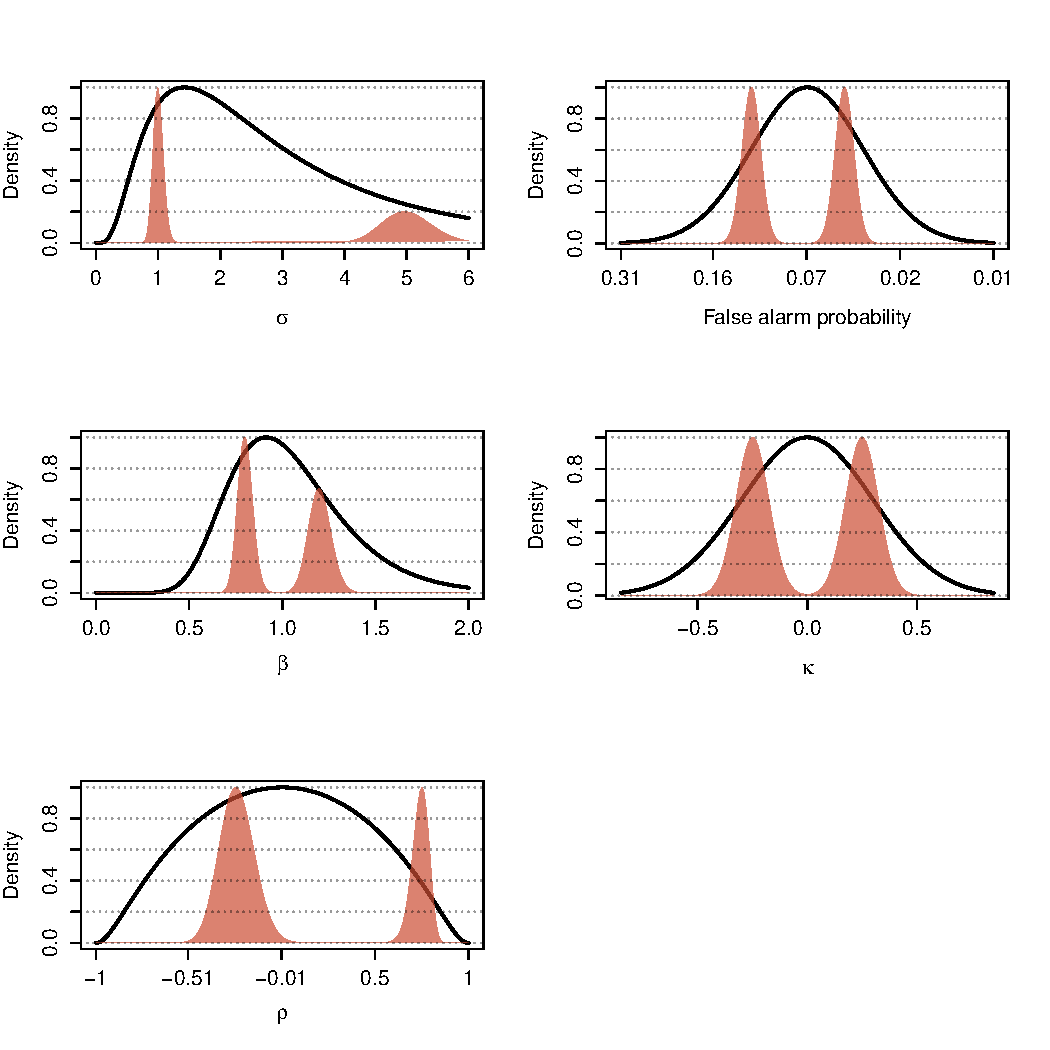
\includegraphics[width=\maxwidth]{figure/unnamed-chunk-16-1} 

\end{knitrout}

\caption{Examples of stimuli used in the psychophysical experiment. In both panels $F_1 = 150\text{Hz}$. Spectral prominence in upper panel is 850Hz and in lower panel 1300Hz, making the stimulus in the lower panel brighter in timbre.}
\label{fig:stimuli}
\end{figure}


%!Rnw root = ../Joni_Paakko_-_Thesis.Rnw

\subsection{Results} 

Some model development was inevitable in order to fit the psychophysical data. All of the models are presented  in Table \ref{tab:models}. Note that the models for the Yes/No and 2I-4AFC tasks are identical save for the AFC models lacking the criterion parameters. 

Model fits for both participants are presented separately. Analysis for both participants is divided into two stages, the first describing models 1 to 3 and the second a model in which both kinds of interactions are present. I've also included short discussions of the models alongside the results, to act as a roadmap through the model fitting/development process; general discussion about the main questions is reserved for later. 

I will also present the reader with some introspective remarks, to act as qualitative model criticism.  

\begin{table}
\caption{All of the models fitted to the psychophysical data. If other information is not present, an X indicates that the parameter(s) are free in the model. }
\vspace{0.5cm}
\begin{adjustbox}{center}
\begin{tabular}{rrccccccc}

\toprule

  &       & \multicolumn{7}{c}{Parameters} \\
\cmidrule(lr){3-9}  
 Task & Model & $\sigma$ & C & $\beta$ & $\kappa_{\mu}$ & $\kappa_{\sigma}$ & $\rho$ & $\lambda$ \\
\midrule
\multirow{5}{*}{\rotatebox[origin=c]{90}{Yes/No}} & Model 1 & X & X & X & X &   & X & Fixed ($\lambda = 0.02$) \\
& Model 2 & X & Wider prior & X & X &   & X & X \\
& Model 3 & X & Wider prior & X &   & X  & X & X \\
& Both    & X & Wider prior & X & X & X  & $-0.8 < \rho < 0.8$ & X \\
& Both (Truncated) & X & Wider prior & X & X & $\kappa_{\sigma} > 0$  & $-0.8 < \rho < 0.8$ & X \\

\hline

\multirow{5}{*}{\rotatebox[origin=c]{90}{2I-4AFC}} & Model 1 & X &   & X & X &   & X & Fixed ($\lambda = 0.02$) \\
& Model 2 & X &   & X & X &   & X & X \\
& Model 3 & X &   & X &   & X  & X & X \\
& Both    & X &   & X & X & X  & $-0.8 < \rho < 0.8$ & X \\
& Both (Truncated) & X &  & X & X & $\kappa_{\sigma} > 0$  & $-0.8 < \rho < 0.8$ & X \\

\bottomrule

\end{tabular}
\end{adjustbox}

\label{tab:models}
\end{table}

Models one to three present the initial stage of model development: Model 1 is the same as the one used in simulations. For models 2 and 3 the parameter $\lambda$ was estimated from the data, to accomodate the (presumably) higher proportion of lapsing trials than assumed a prior; also the prior for the criterion was widened, again, to better accomodate smaller false alarm probabilities. Model 3 uses the $\kappa_{sigma}$ style model of interference. 

The model labelled \textit{Both} has, as the name implies, both kinds of interferences in it. The last model, \textit{Both (Truncated)} is otherwise identical to the previous model, but the $\kappa{sigma}$ is bound to positive values. For these models also the parameter $\rho$ was bound between -0.8 and 0.8 to improve computational stability: for the model with normal prior on tanh transformed scale the chains of the MCMC sampler sometimes get stuck to extreme values of correlation.

All of the models are included in the appendix, the naming convention follows the one established in this section. 

\subsubsection{Posterior predictive plots}

I did model checking by dividing the two dimensional space of stimuli into three bins per dimension, resulting into 9 total bins, and calculating the proportion of positive responses in each bin for both dimensions. In the data from the Yes/No task the first bin always included stimuli with strength 0.

This method resulted in unequal bin sizes and I would recommend that future works use more sophisticated methods for finding boundaries for the bins. 

In all of the posterior predictive plots (see for example Figure \ref{fig:OK_YN_post_pred}) the black dots joined by the dashed lines indicate observed data. For example in the top left of Figure \ref{fig:OK_YN_post_pred} the first three black dots indicate responses to increasingly large pitch changes pitch when timbre category is 1 (no change in timbre), the next three dots indicate response to pitch when timbre category is 2 (some change in timbre) and so on. 

In this exemplar figure one can can see that in each timbre category the probability of a positive response to a pitch change increases when the pitch differences get larger. However, the magnitude changes with the timbre category, indicating some kind of interference between pitch and timbre.

The data, in each case, is also divided by the category of the irrelevant dimension. For example on the upper row probability of a positive response to pitch dimension (relevant dimension) is plotted. These are broken down with regards to timbre (irrelevant dimension). Inside each timbre category, pitch category goes up from left to right. 

Since completely straight and orthogonal boundaries were used for binning the data, the number of observations per bin varied somewhat; for the participant JP, there didn't seem to be bounds that would result in better distribution. Another factor leading to uneven bin sizes was my decision to bin stimuli with strength 0 in the YN task separately. Number of observations per bin are reported in Table \ref{tab:binsizes}.

\begin{table}
\caption{Number of observations per bin in the posterior predictive distribution.}
\vspace{0.5cm}
\centering
\begin{tabular}{rrrccccccccc}

\toprule

\multirow{2}{*}{\rotatebox[origin=c]{90}{Bin}} & \multicolumn{2}{r}{Pitch} & 1 & 1 & 1 & 2 & 2 & 2 & 3 & 3 & 3 \\
& \multicolumn{2}{r}{Timbre} & 1 & 2 & 3 & 1 & 2 & 3 & 1 & 2 & 3 \\

\midrule

\multirow{4}{*}{\rotatebox[origin=c]{90}{N}} & \multirow{2}{*}{JP} & YN & 108 & 58 & 49 & 53 & 38 & 6 & 50 & 6 & 32 \\
& & AFC & 48 & 81 & 21 & 68 & 38 & 24 & 26 & 34 & 60 \\

\cmidrule(lr){2-12}

& \multirow{2}{*}{OK} & YN & 111 & 39 & 50 & 49 & 38 & 14 & 50 & 18 & 31 \\
& & AFC & 105 & 27 & 20 & 45 & 80 & 16 & 12 & 16 & 79 \\

\end{tabular}
\label{tab:binsizes}
\end{table}

\subsubsection{Participant OK, Models 1 to 3}

\begin{figure}[H]
\centering
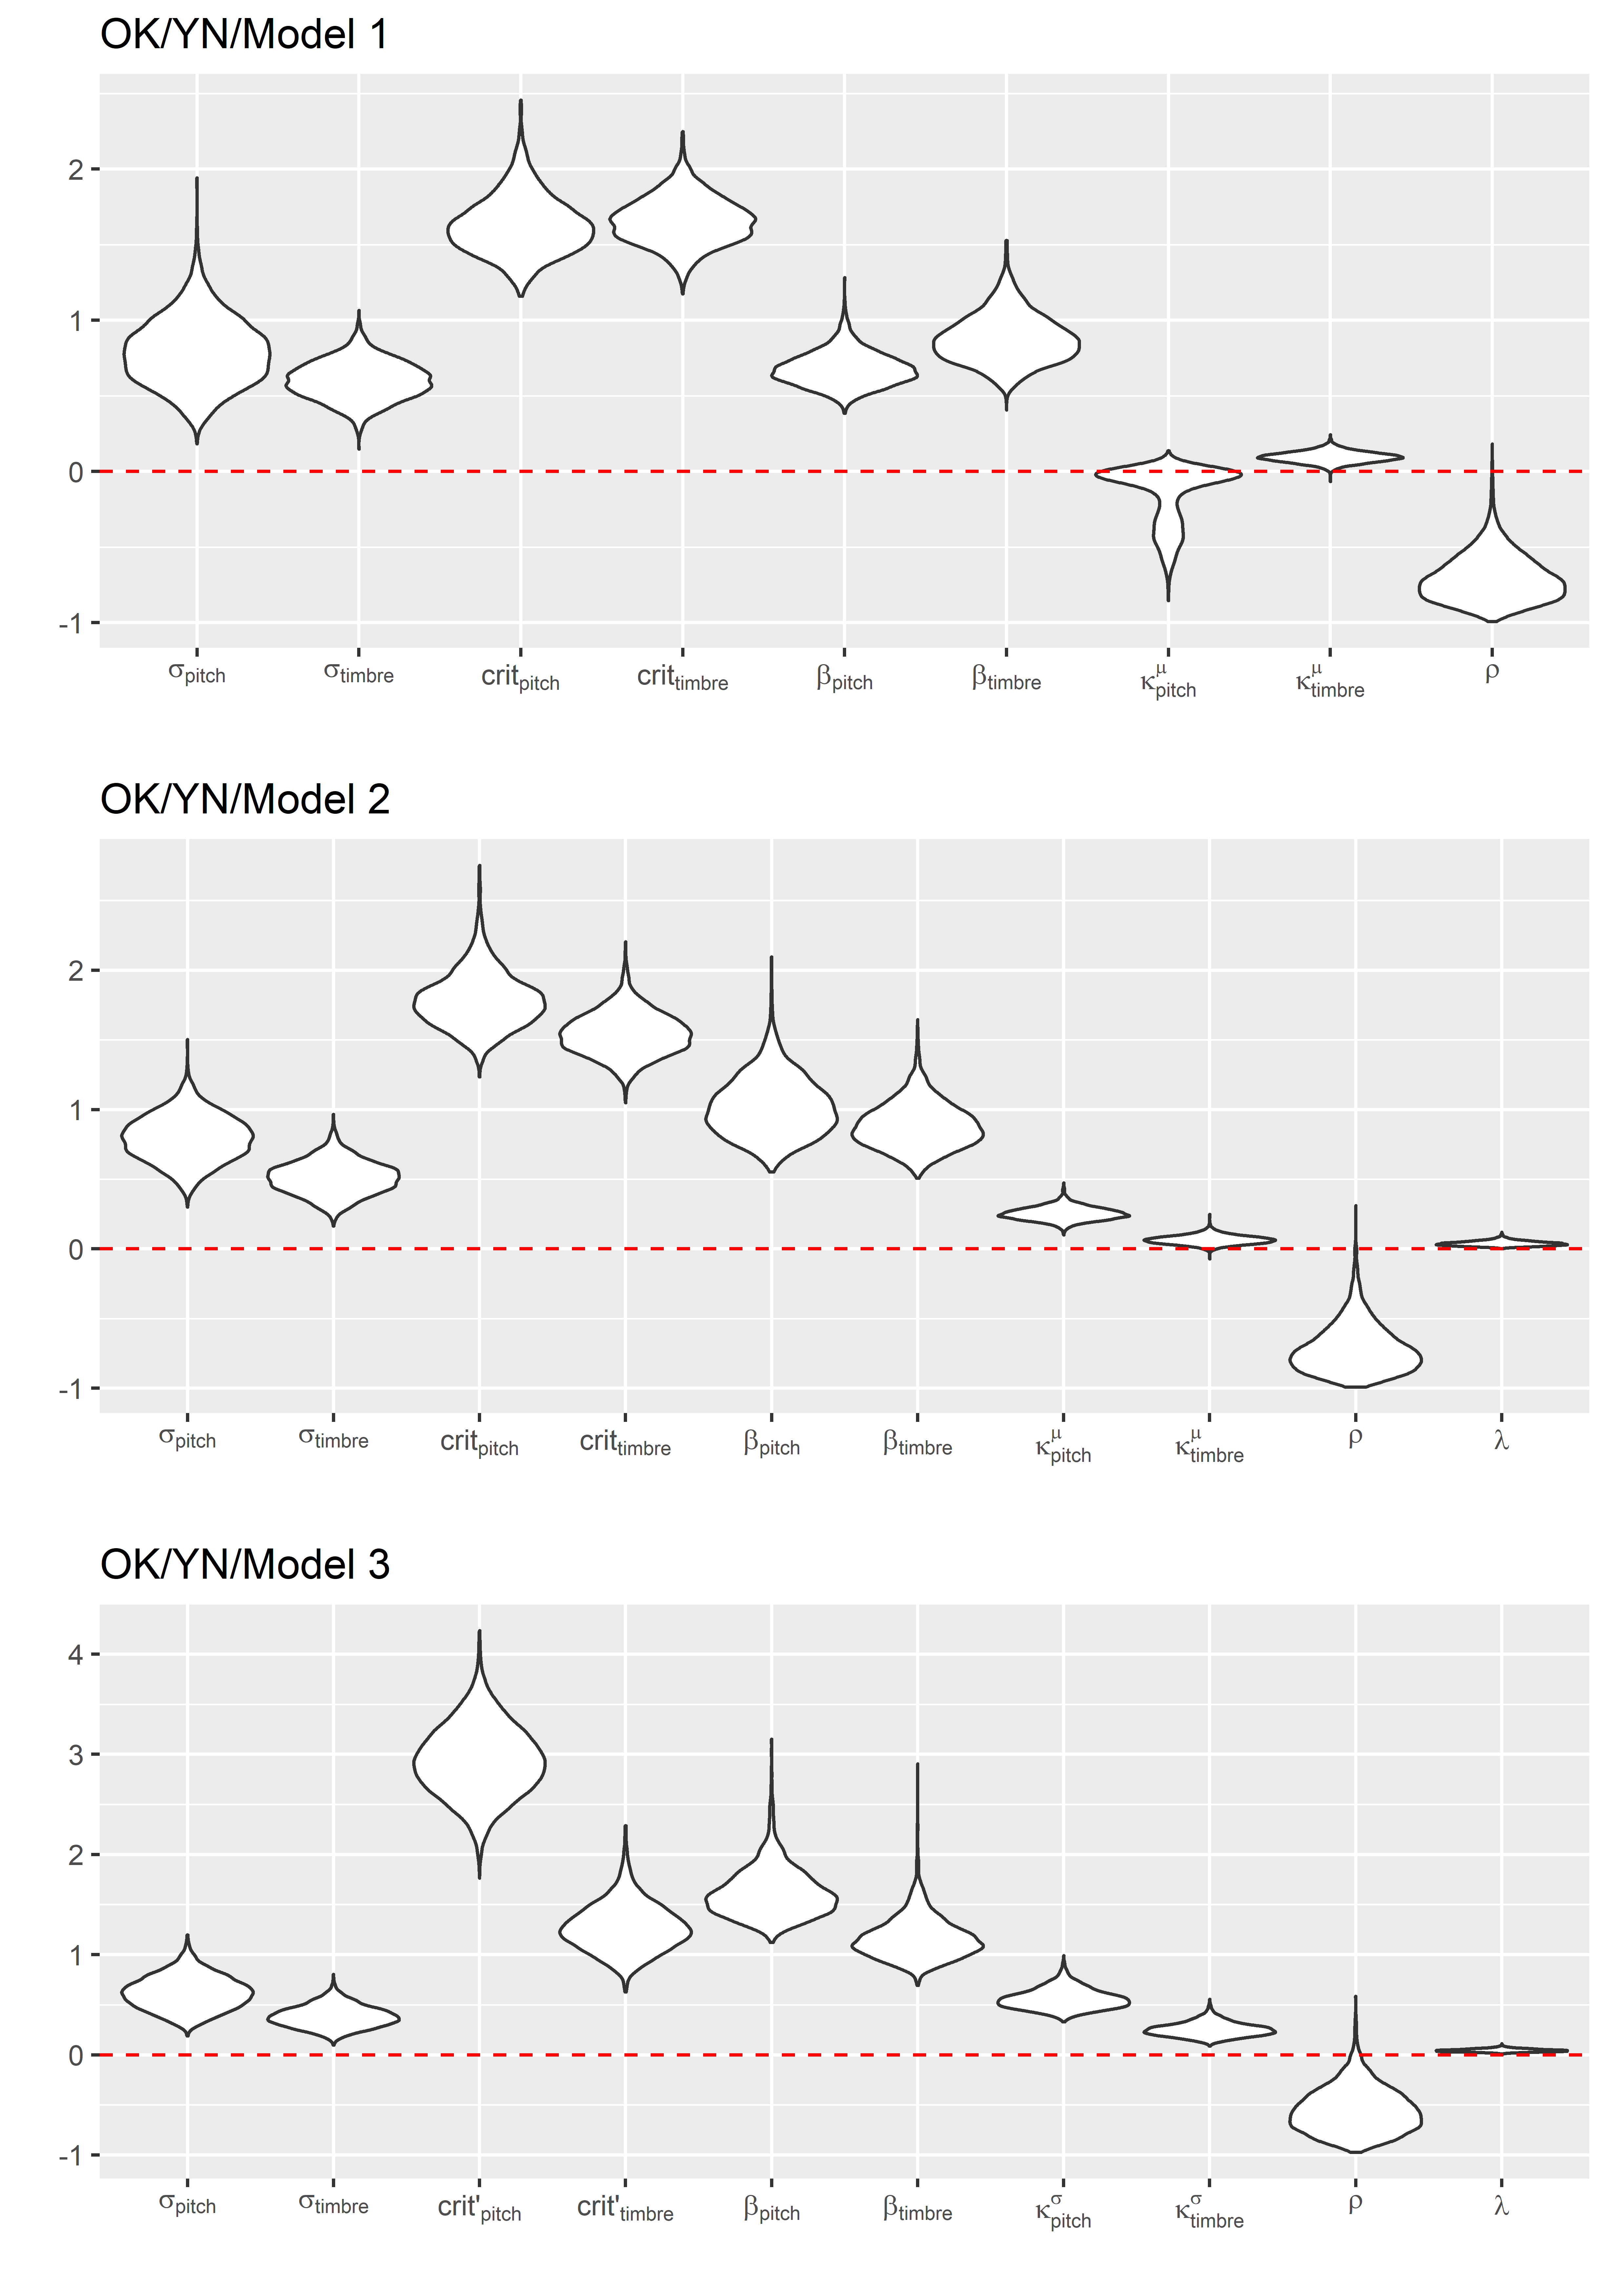
\includegraphics[scale=0.75, angle = 0]{Analysis_of_Human_Data/OK_YN_Basic_models}
\caption{Task: Yes/No; Participant: OK. Marginal posterior distributions for parameters of Models 1 to 3.}
\label{fig:OK_YN_Basic_models}
\end{figure}

\begin{figure}[H]
\centering
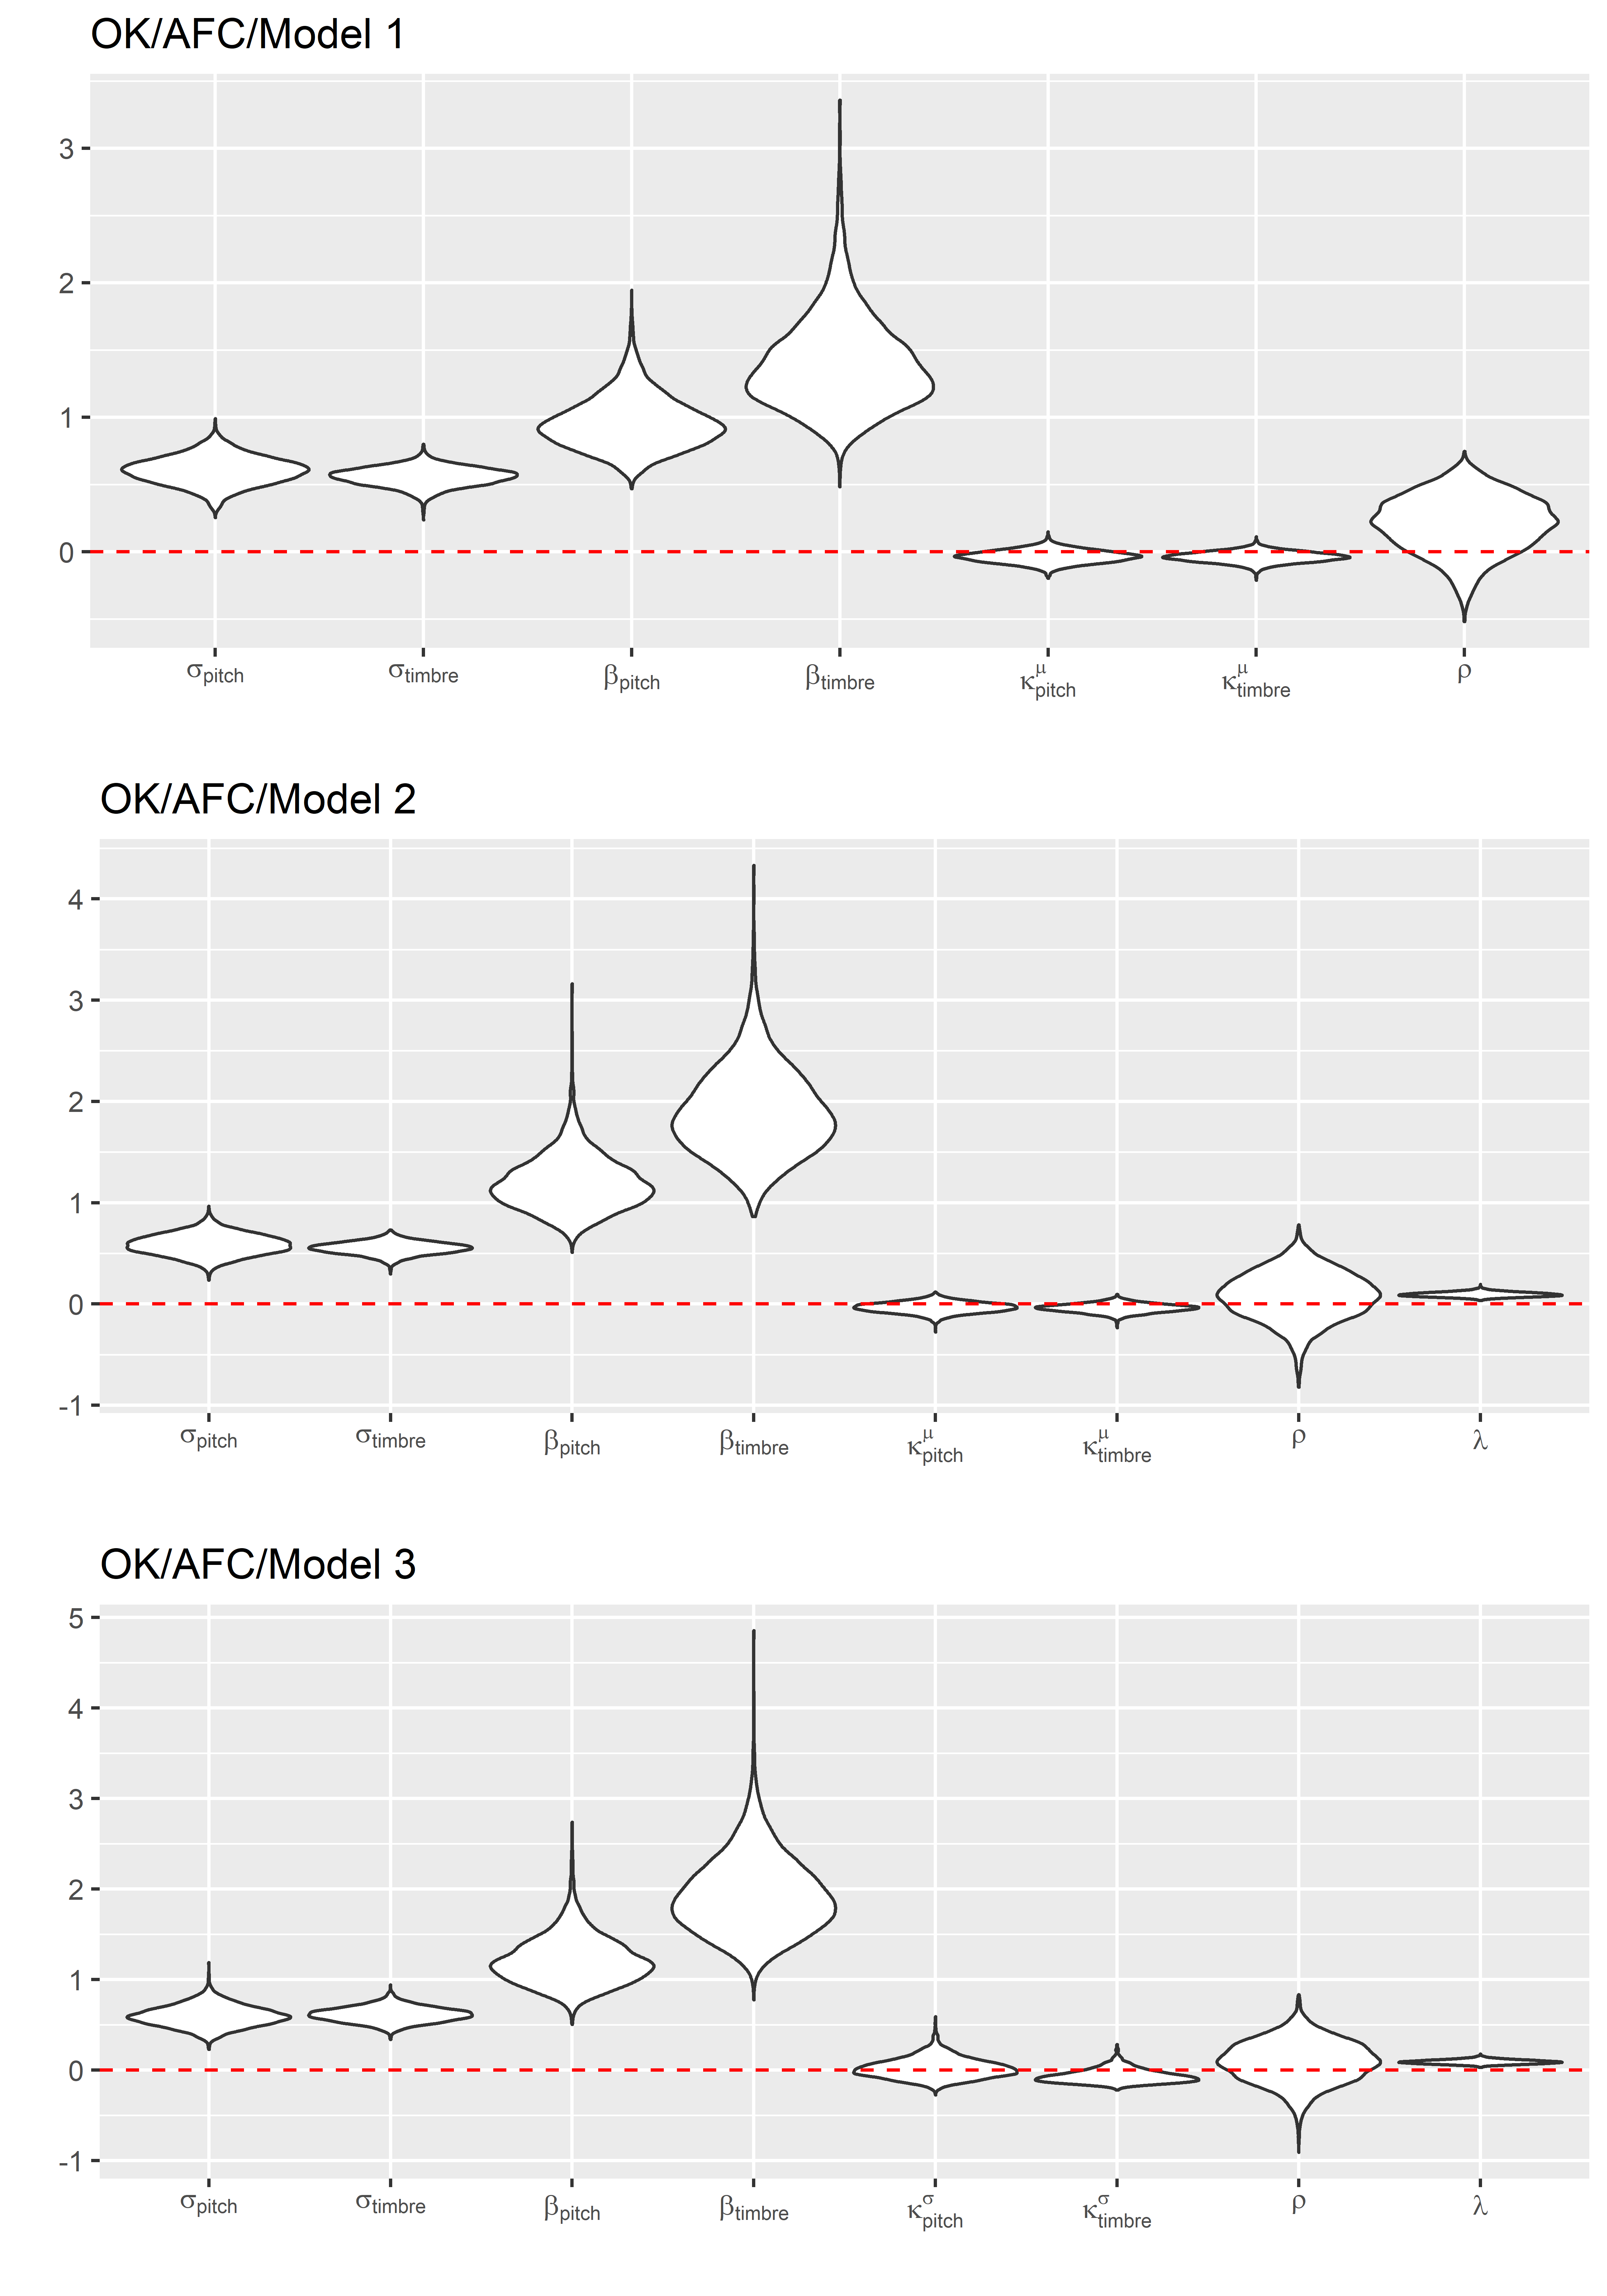
\includegraphics[scale=0.75, angle = 0]{Analysis_of_Human_Data/OK_AFC_Basic_models}
\caption{Task: 2I-4AFC; Participant: OK. Marginal posterior distributions for parameters of Models 1 to 3.}
\label{fig:OK_AFC_Basic_models}
\end{figure}

\begin{figure}[H]
\centering
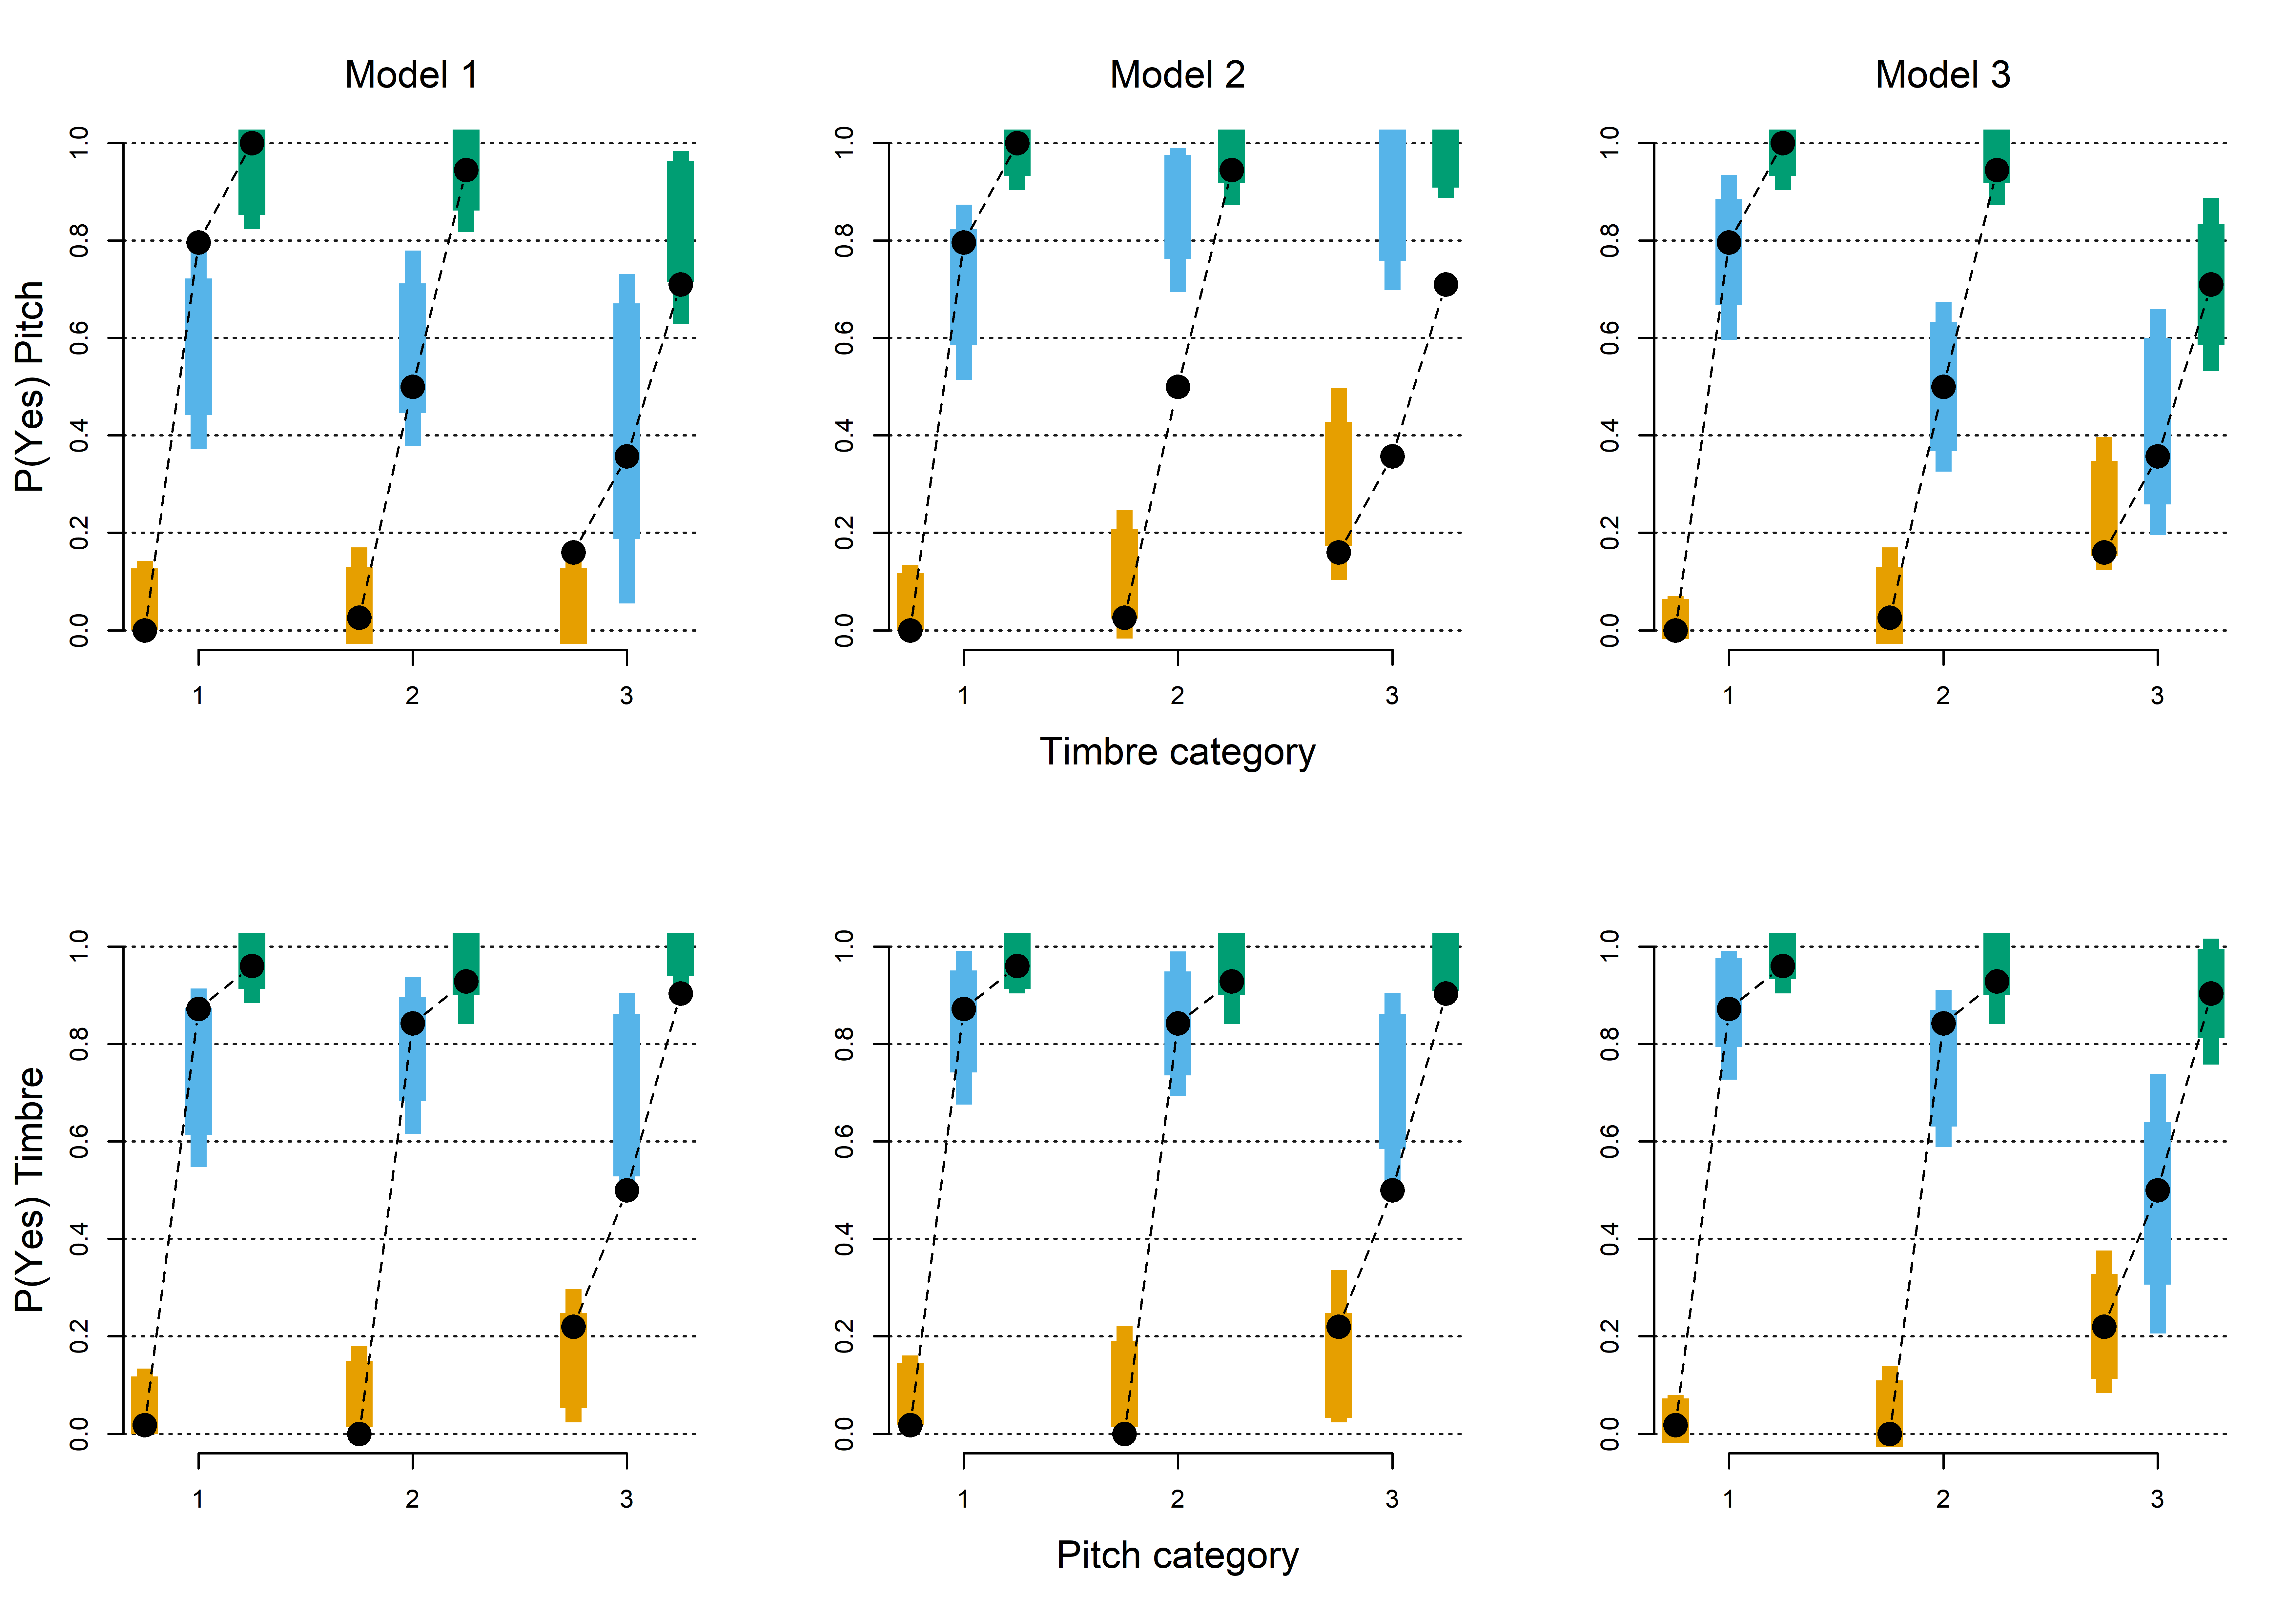
\includegraphics[scale=0.75, angle = 270]{Analysis_of_Human_Data/OK_YN_post_pred}
\caption{Task: Yes/No; Participant: OK. Posterior predictive distributions for parameters of Models 1 to 3.}
\label{fig:OK_YN_post_pred}
\end{figure}

\begin{figure}[H]
\centering
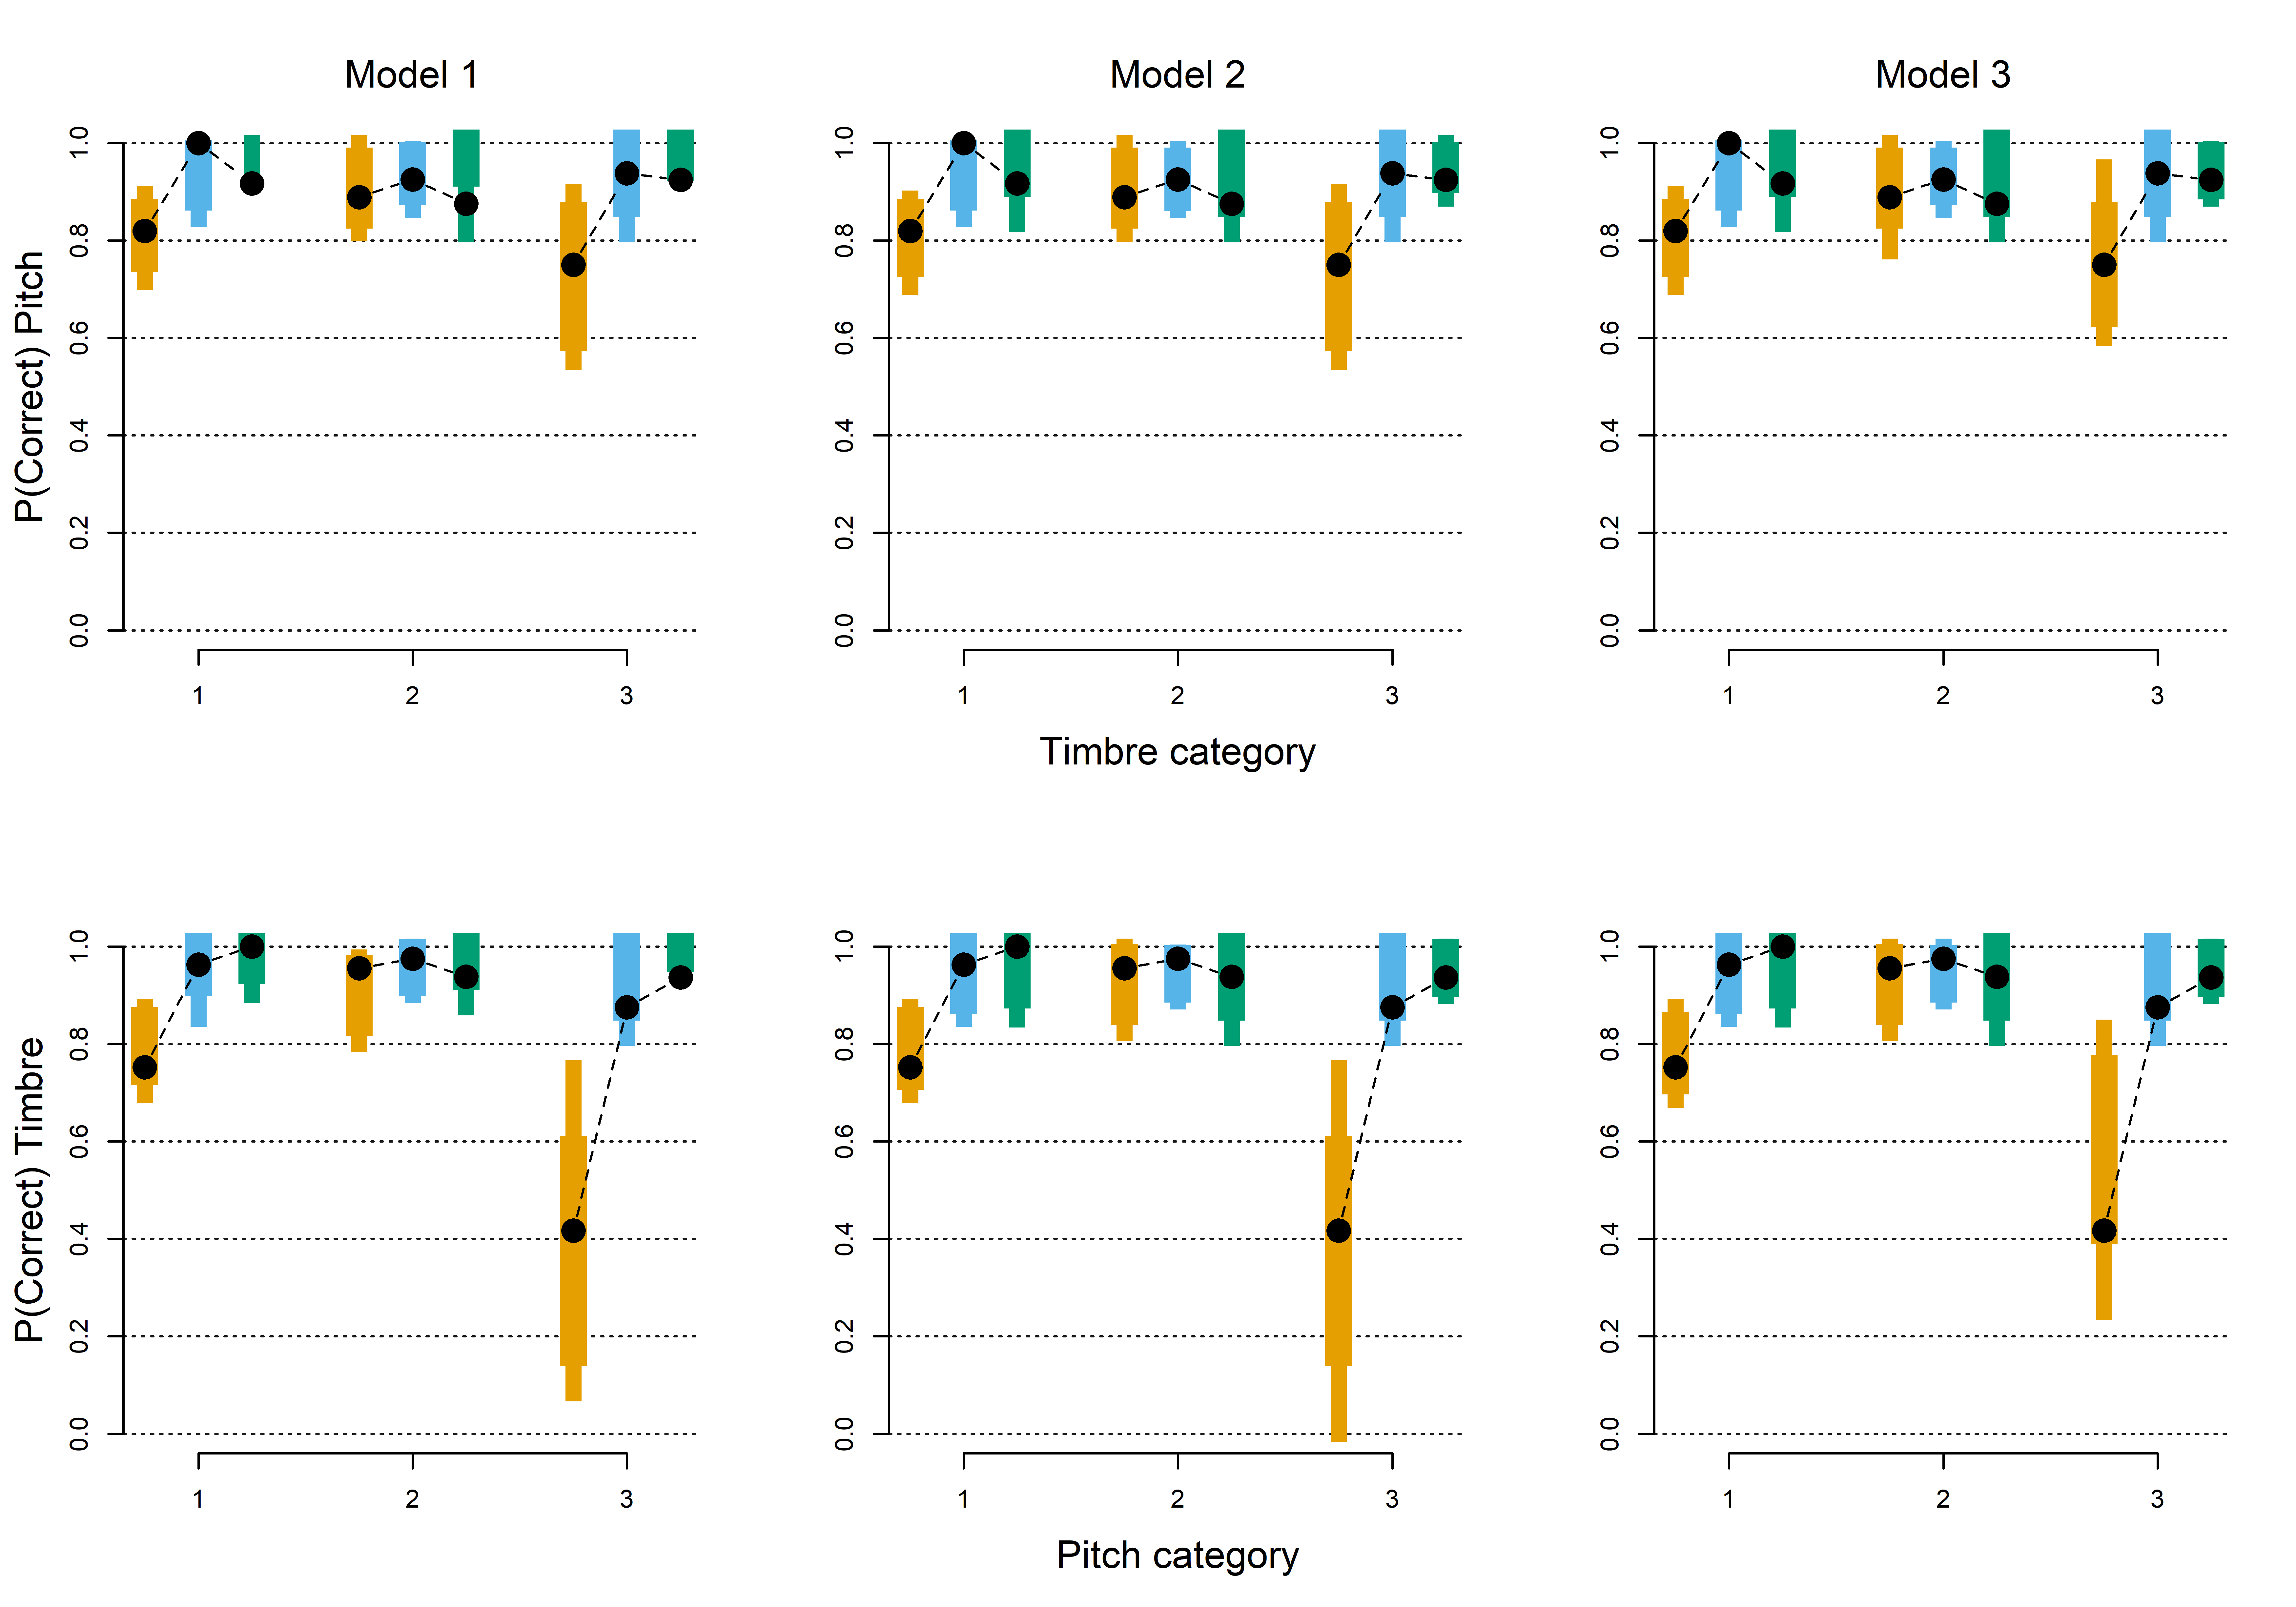
\includegraphics[scale=0.75, angle = 270]{Analysis_of_Human_Data/OK_AFC_post_pred}
\caption{Task: 2I-4AFC; Participant: OK. Posterior predictive distributions for parameters of Models 1 to 3.}
\label{fig:OK_AFC_post_pred}
\end{figure}

\paragraph{Participant OK, Models 1 to 3: Discussion}

In the Yes/No task, it is apparent from the bimodality of the posterior distribution for the $\kappa_{mu}$ parameter (Figure \ref{fig:OK_YN_Basic_models}, top panel) that there are problems with Model 1. Freeing the $\lambda$ parameter (Model 2) manages to fix the bimodality for that parameter (centre panel in the same figure), but this affects the posterior predictive performance negatively (Figure \ref{fig:OK_YN_post_pred}, centre panel). 

From looking at the observed responses (Figure \ref{fig:OK_YN_post_pred}) it is clear that as the irrelevant signal level increases, the probability of a \textit{Yes} response goes towards $0.50$ which is more consistent with a shift in \textit{standard deviation}. 

Due to this, model with coupled standard deviations (Model 3) was fit to the data. It is clear from the posterior predictive plots (Figure \ref{fig:OK_YN_post_pred}, right panel) that this has the closest match to the observed data.

The observed false alarm rates were lower than what I had anticipated \textit{a prior}. To alleviate this problem I widened the prior for the criterion for all of the models besides Model 1, which is the original model.

The same set of models was fit to the data from the 2I-4AFC task. However there is much less to be said; none of the models seem to do significantly worse than the others (Figures \ref{fig:OK_AFC_Basic_models} and \ref{fig:OK_AFC_post_pred}).

\subsubsection{Participant OK, Model with both interactions}

\begin{figure}[H]
\centering
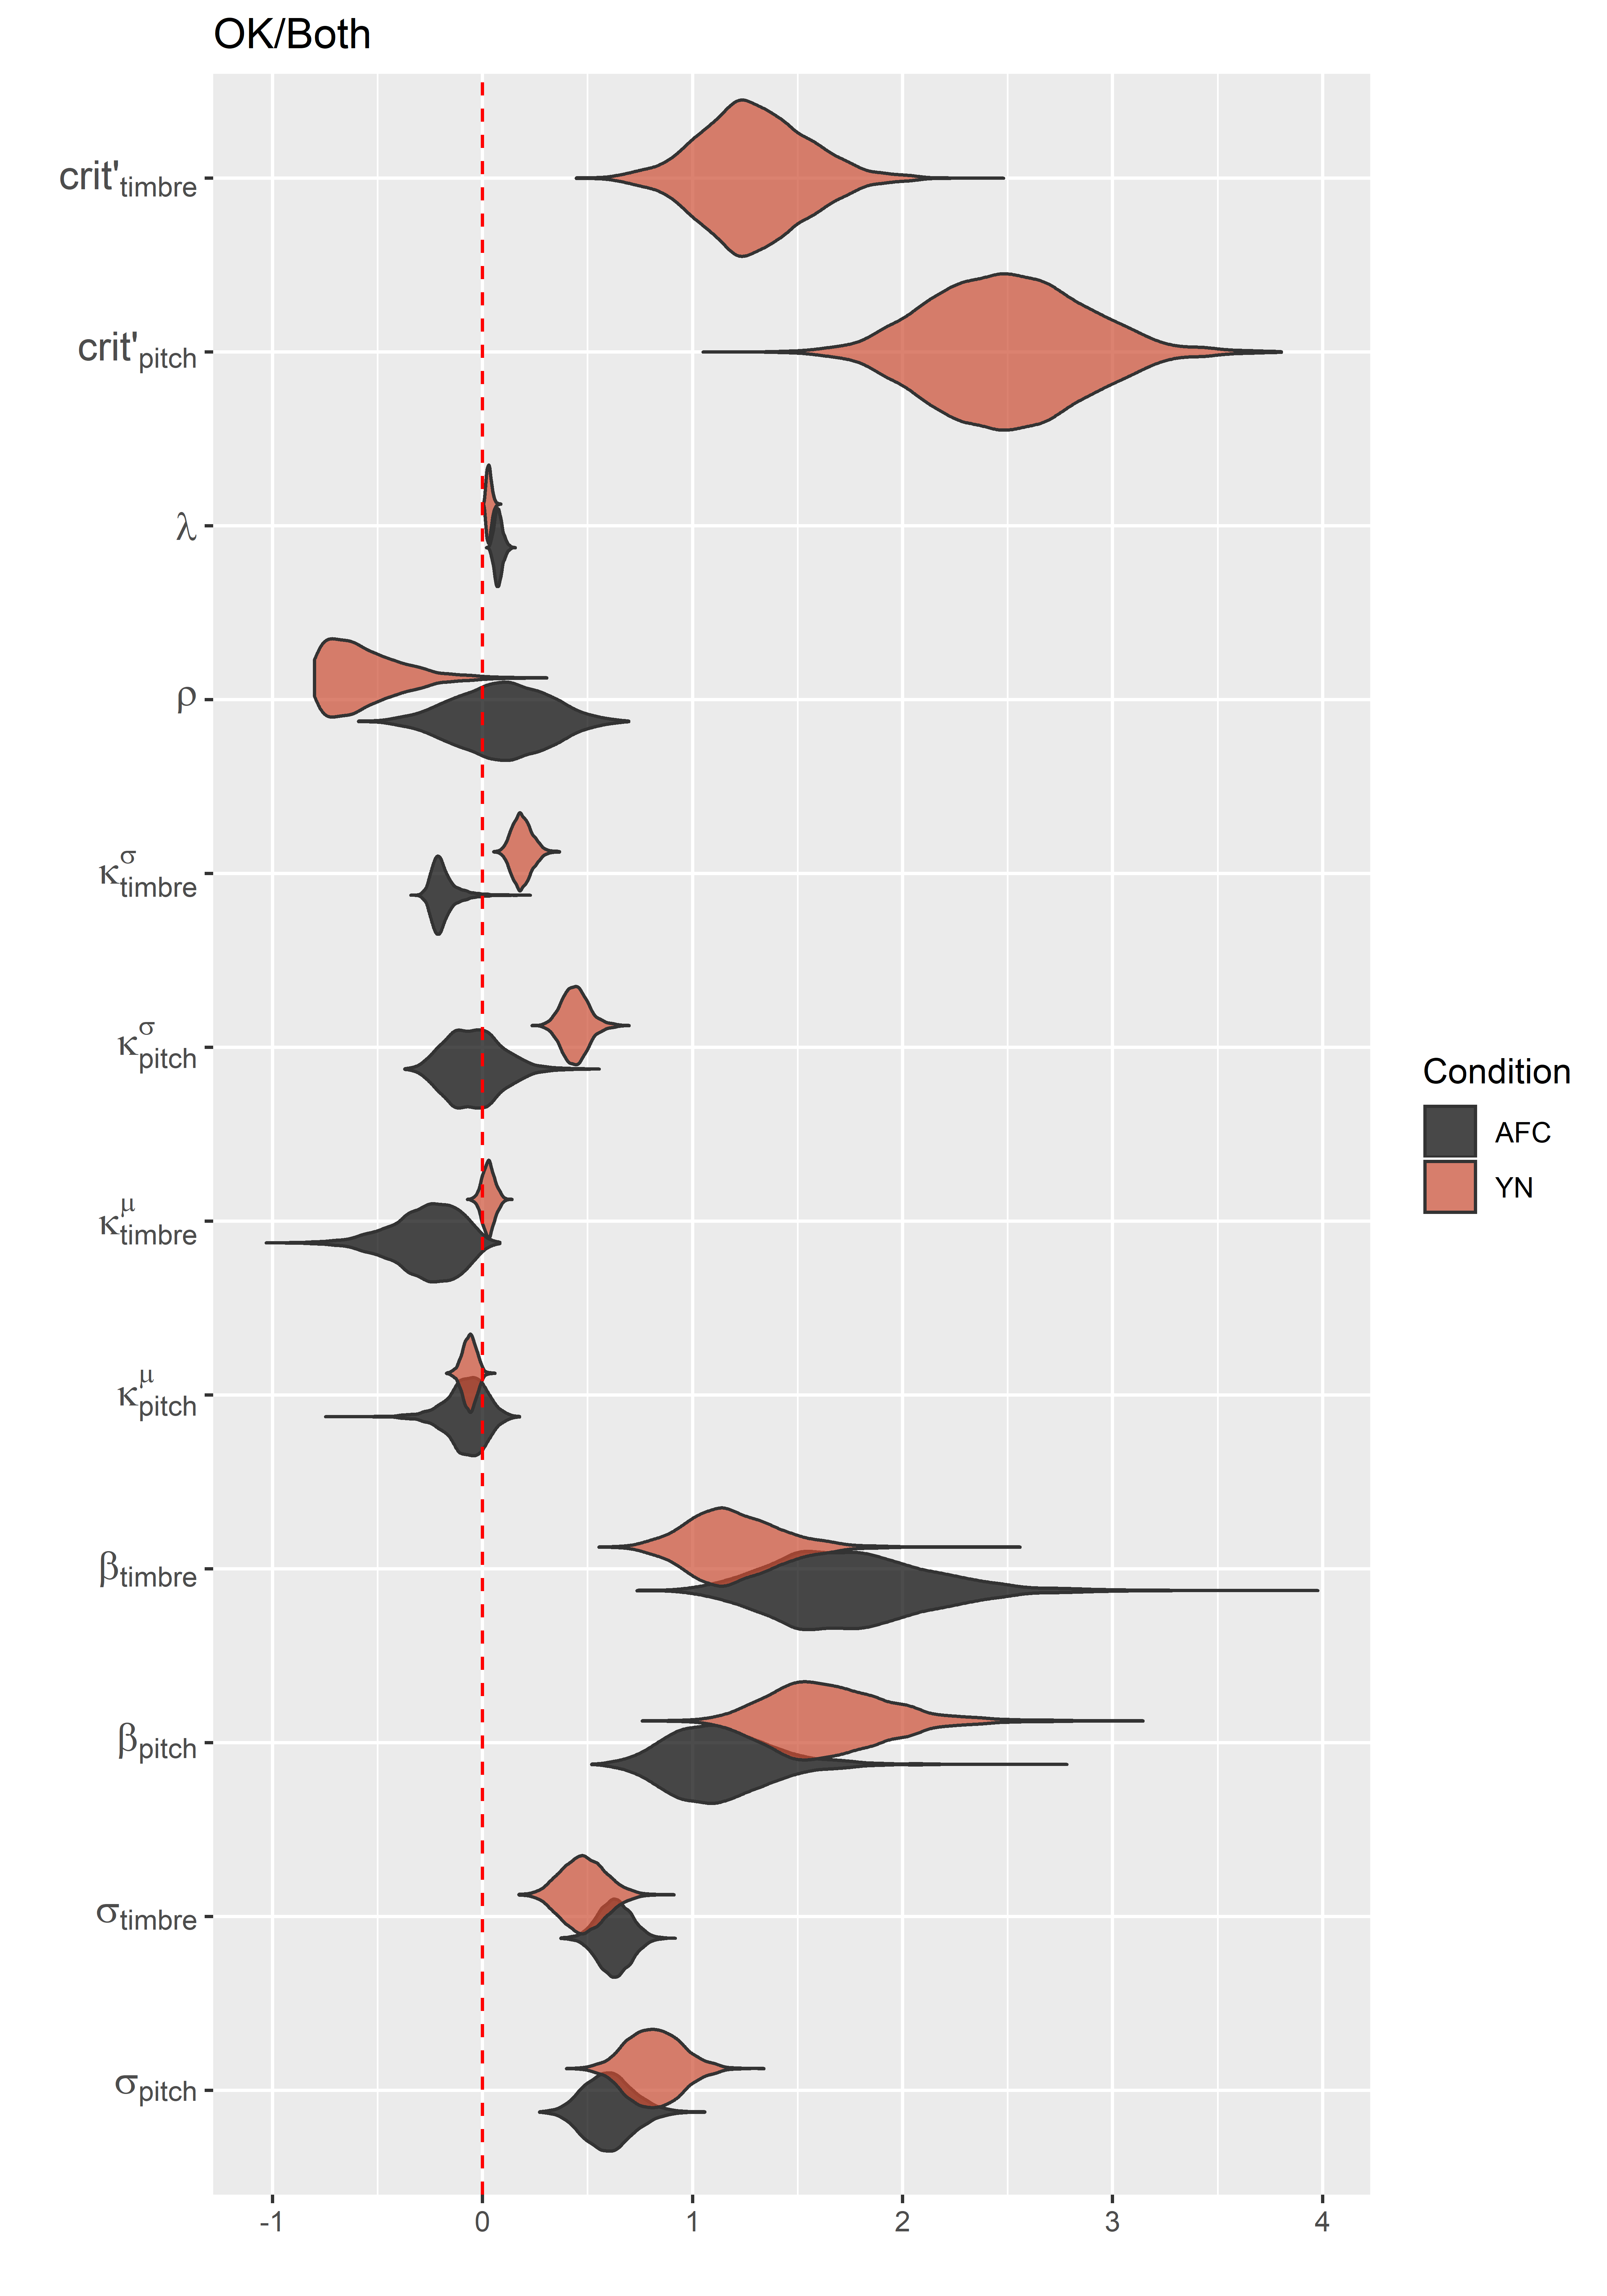
\includegraphics[scale=0.75, angle = 0]{Analysis_of_Human_Data/OK_YN_AFC_Both}
\caption{Both tasks; Participant: OK. Marginal posterior distributions for parameters of model with both interactions}
\label{fig:OK_YN_AFC_Both}
\end{figure}

\begin{figure}[H]
\centering
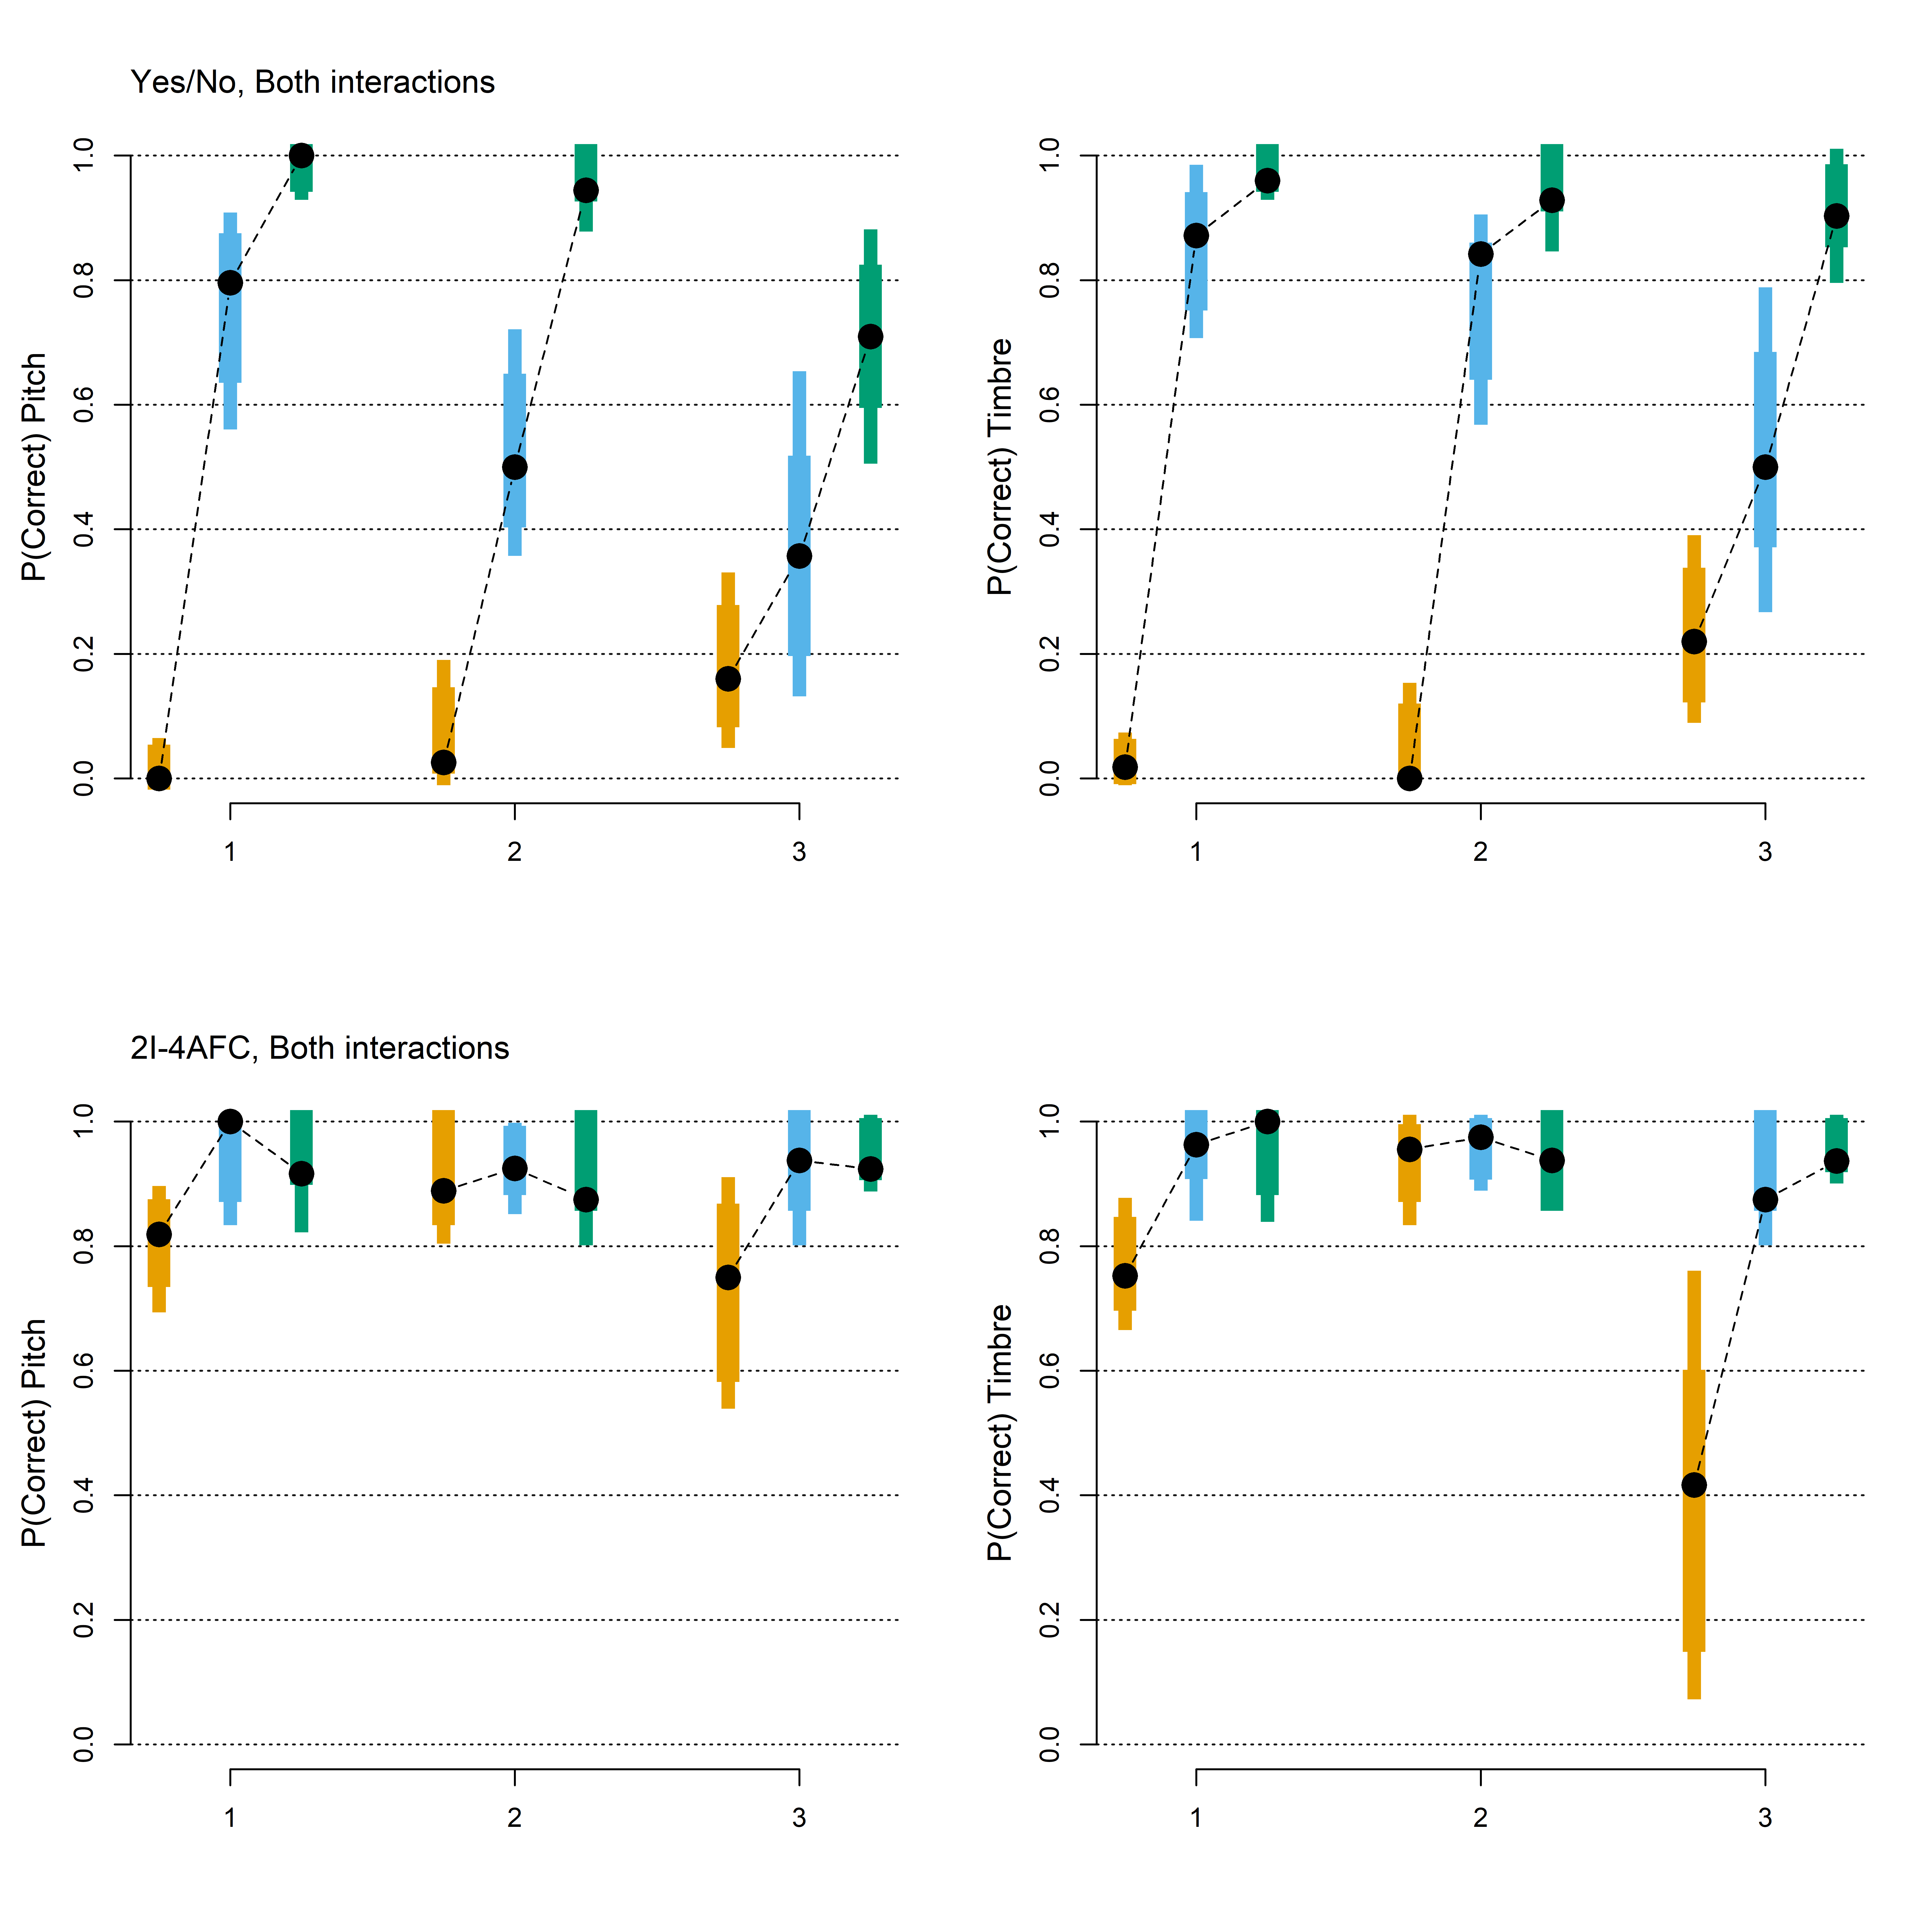
\includegraphics[scale=0.50, angle = 270]{Analysis_of_Human_Data/OK_post_pred_both}
\caption{Both tasks; Participant: OK. Marginal posterior distributions for parameters of model with both interactions}
\label{fig:OK_post_pred_both}
\end{figure}

\paragraph{Participant OK, Model with both interactions: Discussion}

Both kinds of interactions were combined to a single model, in order to compare the relative contributions of both interactions to the observed patterns of inference. Also, one other modification was made: the prior for $\rho$ was changed to a uniform distribution ($\rho \sim \text{Uniform}(-0.8, 0.8)$) since when running the Stan programs, a chain, if it wandered too close to extreme values, would get stuck to those extreme values; the motivation in this  modification, then, was to improve computational stability of the model. 

\subsubsection{Participant JP, Models 1 to 3}

\begin{figure}[H]
\centering
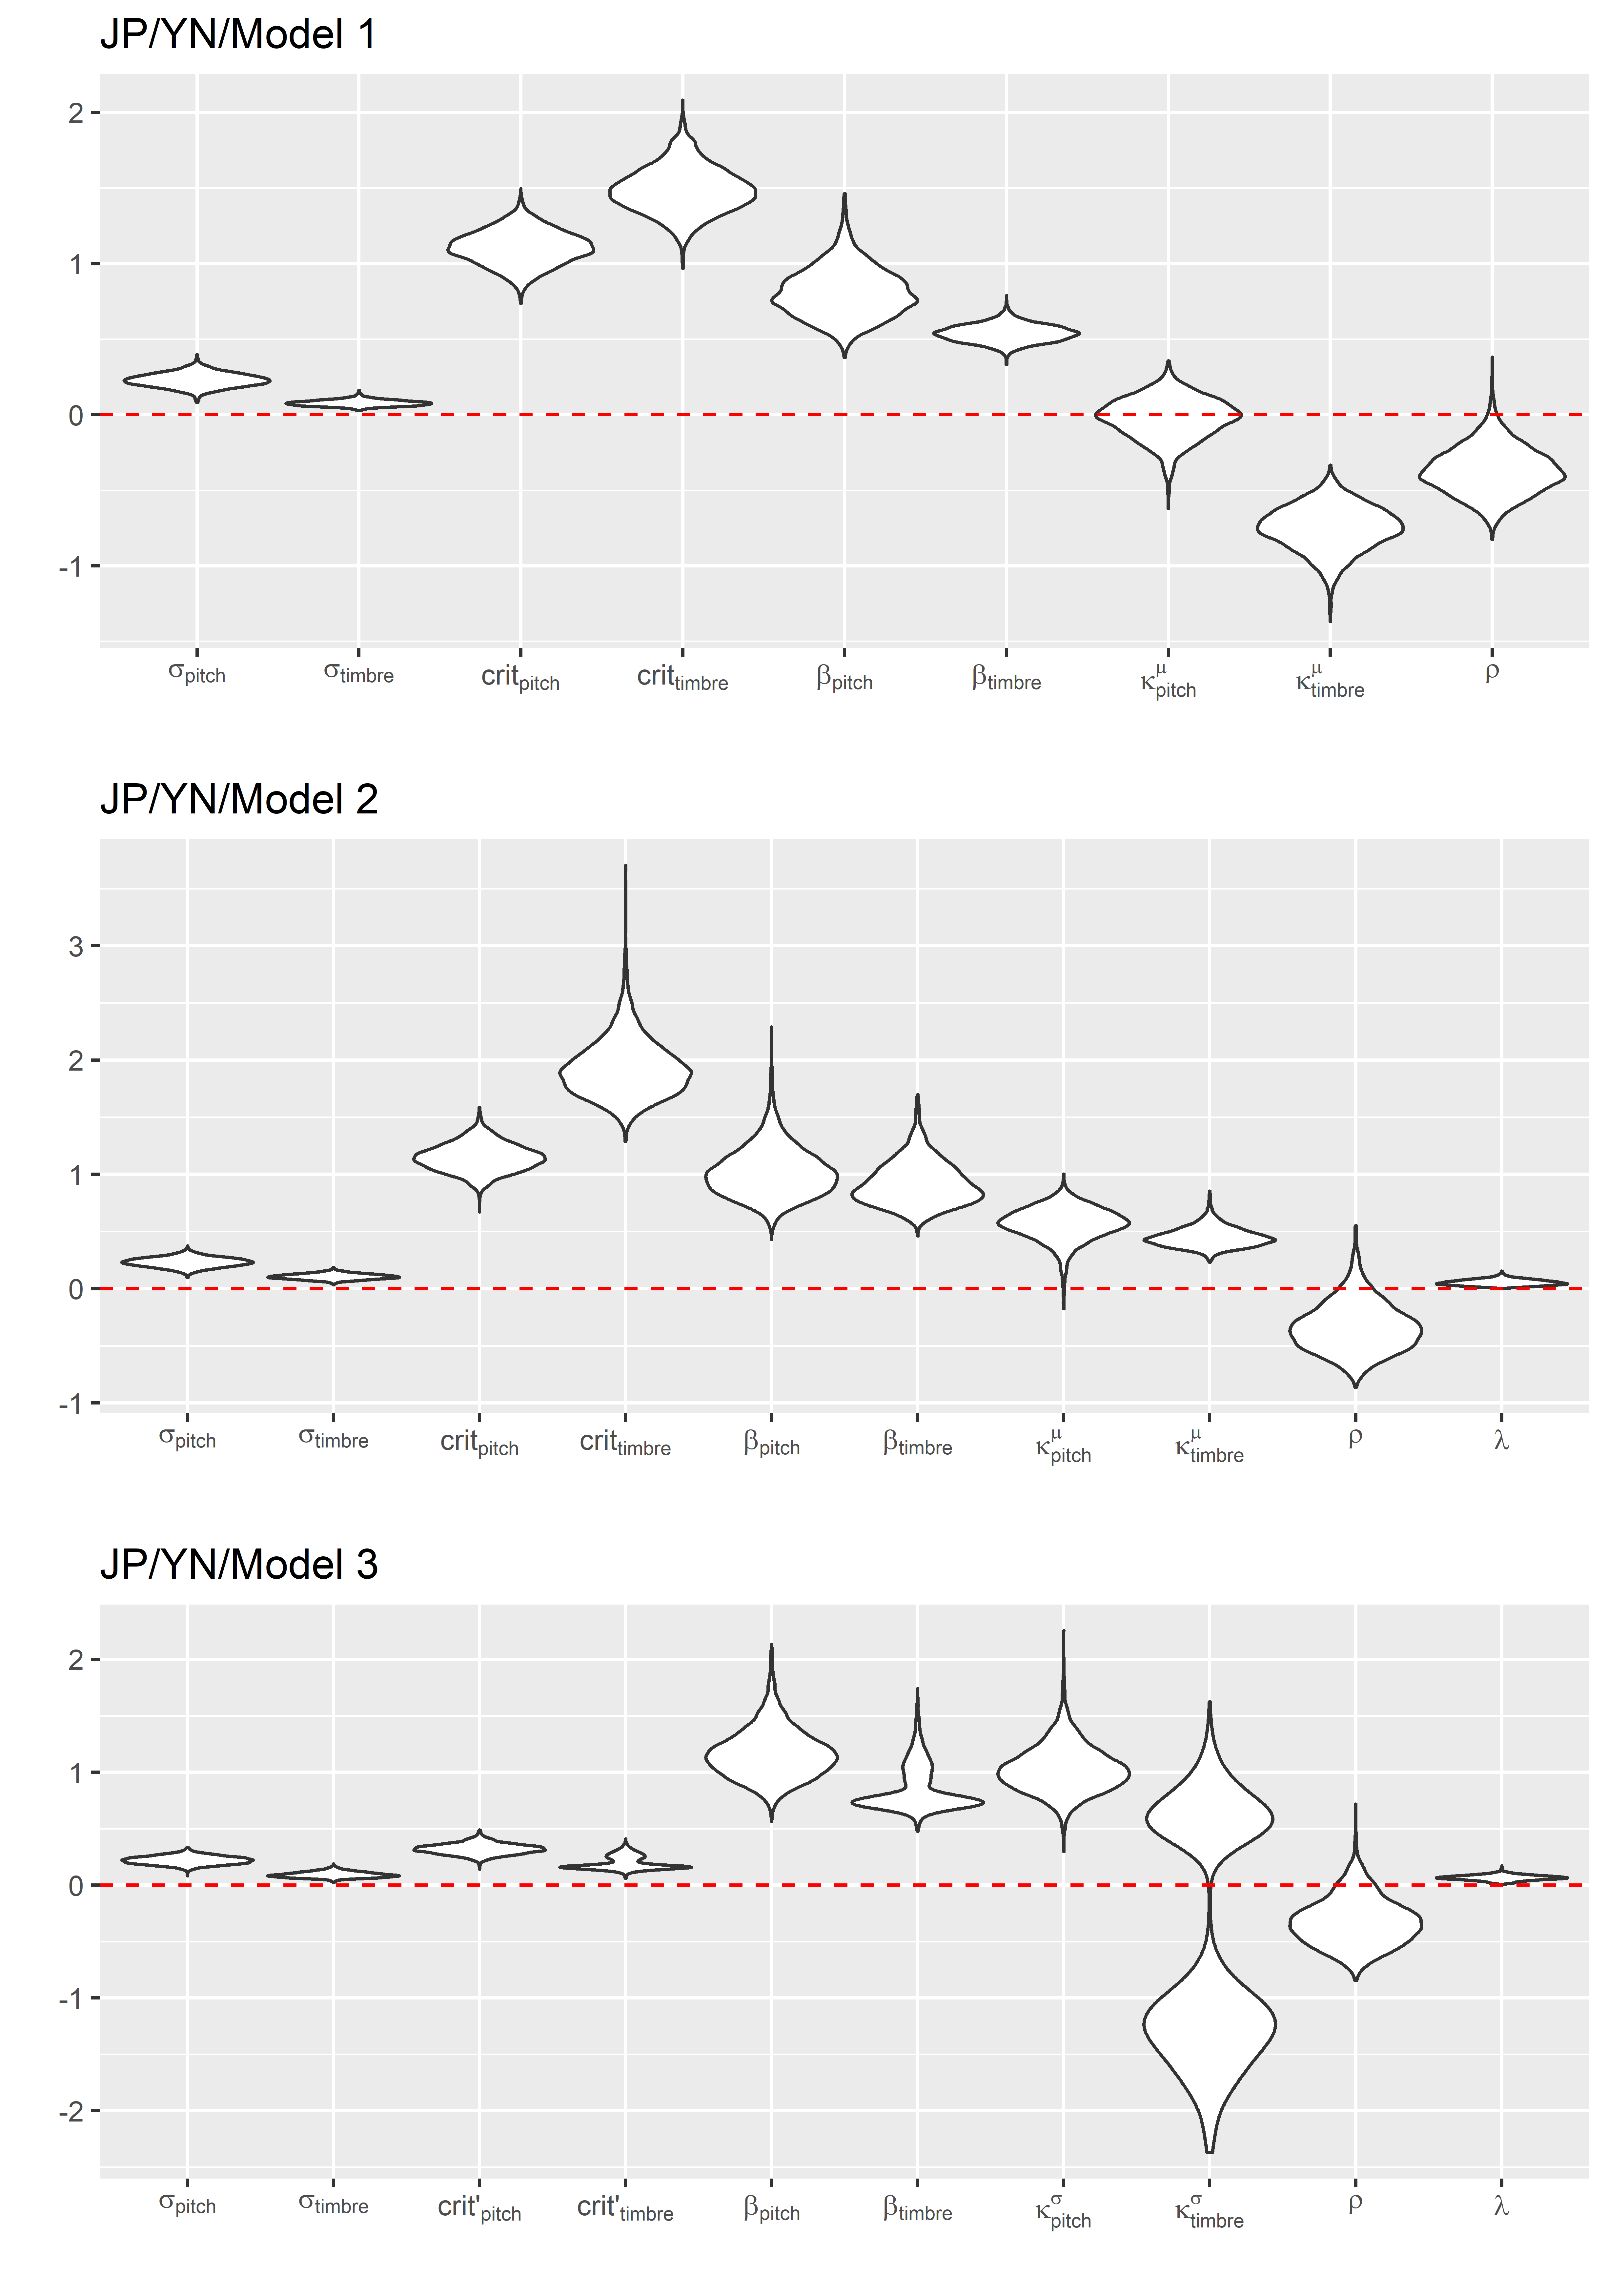
\includegraphics[scale=0.75, angle = 0]{Analysis_of_Human_Data/JP_YN_Basic_models}
\caption{Task: Yes/No; Participant: JP. Marginal posterior distributions for parameters of Models 1 to 3.}
\label{fig:JP_YN_Basic_models}
\end{figure}

\begin{figure}[H]
\centering
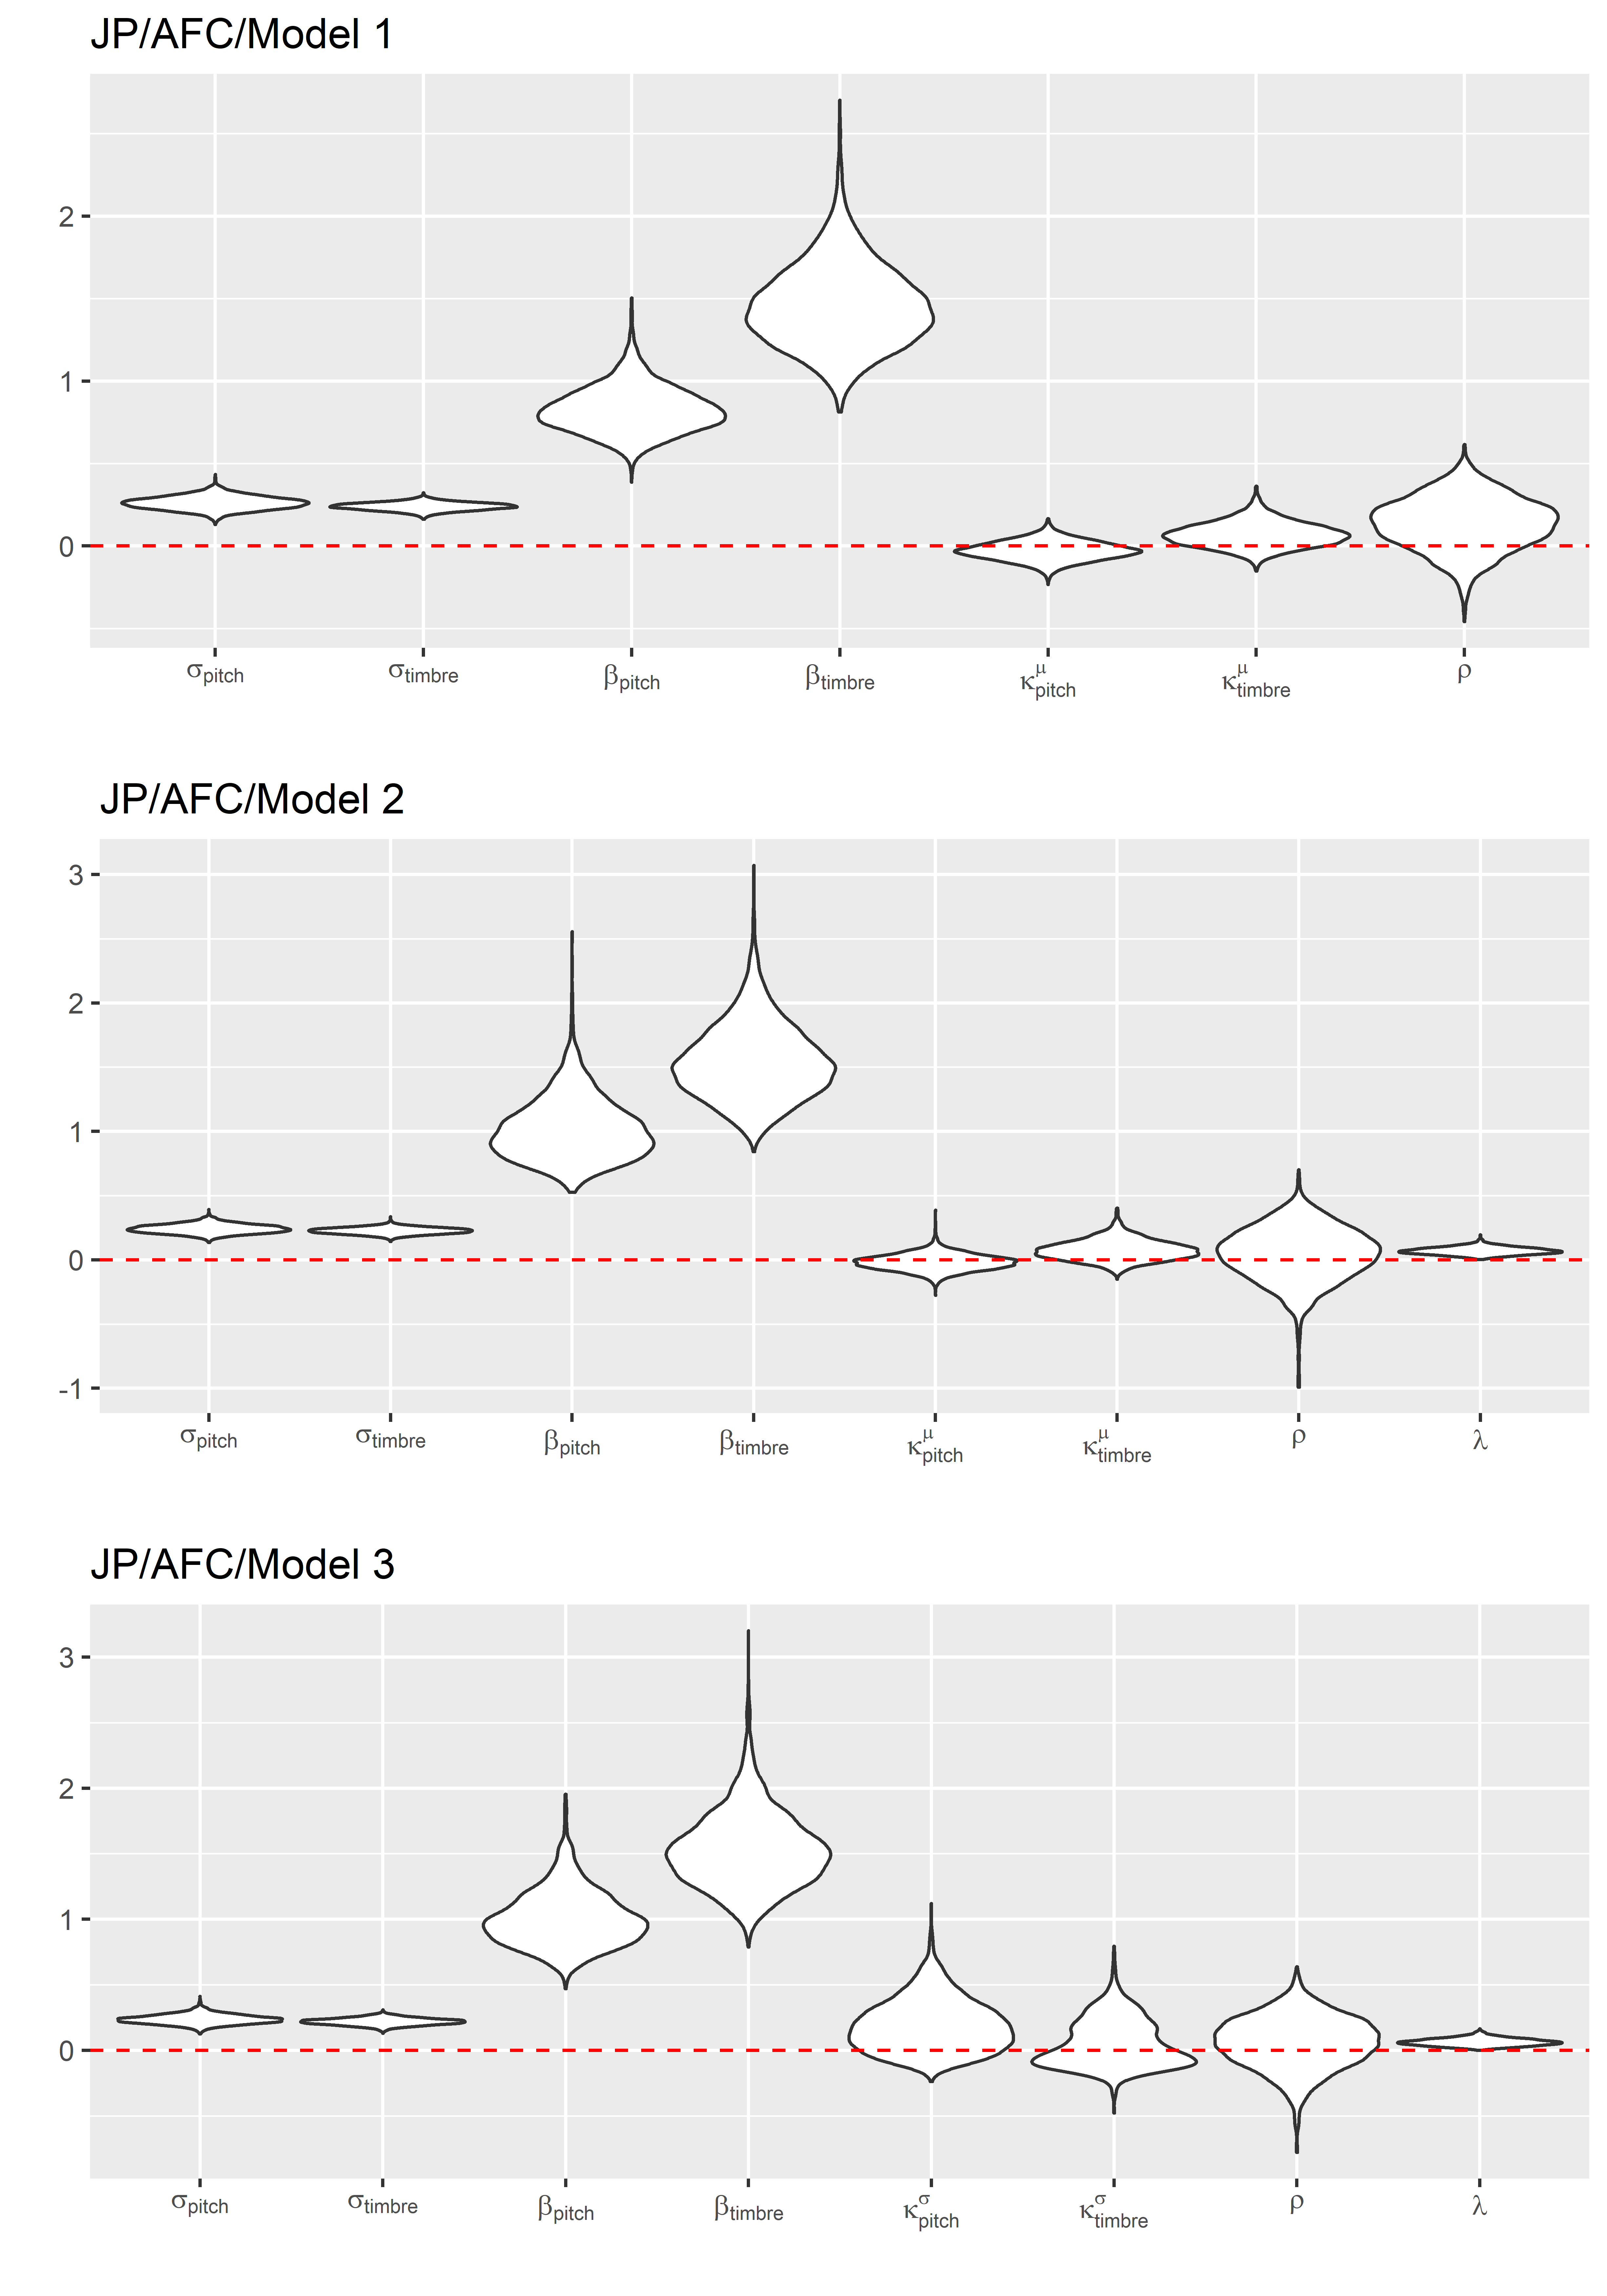
\includegraphics[scale=0.75, angle = 0]{Analysis_of_Human_Data/JP_AFC_Basic_models}
\caption{Task: 2I-4AFC; Participant: JP. Marginal posterior distributions for parameters of Models 1 to 3.}
\label{fig:JP_AFC_Basic_models}
\end{figure}

\begin{figure}[H]
\centering
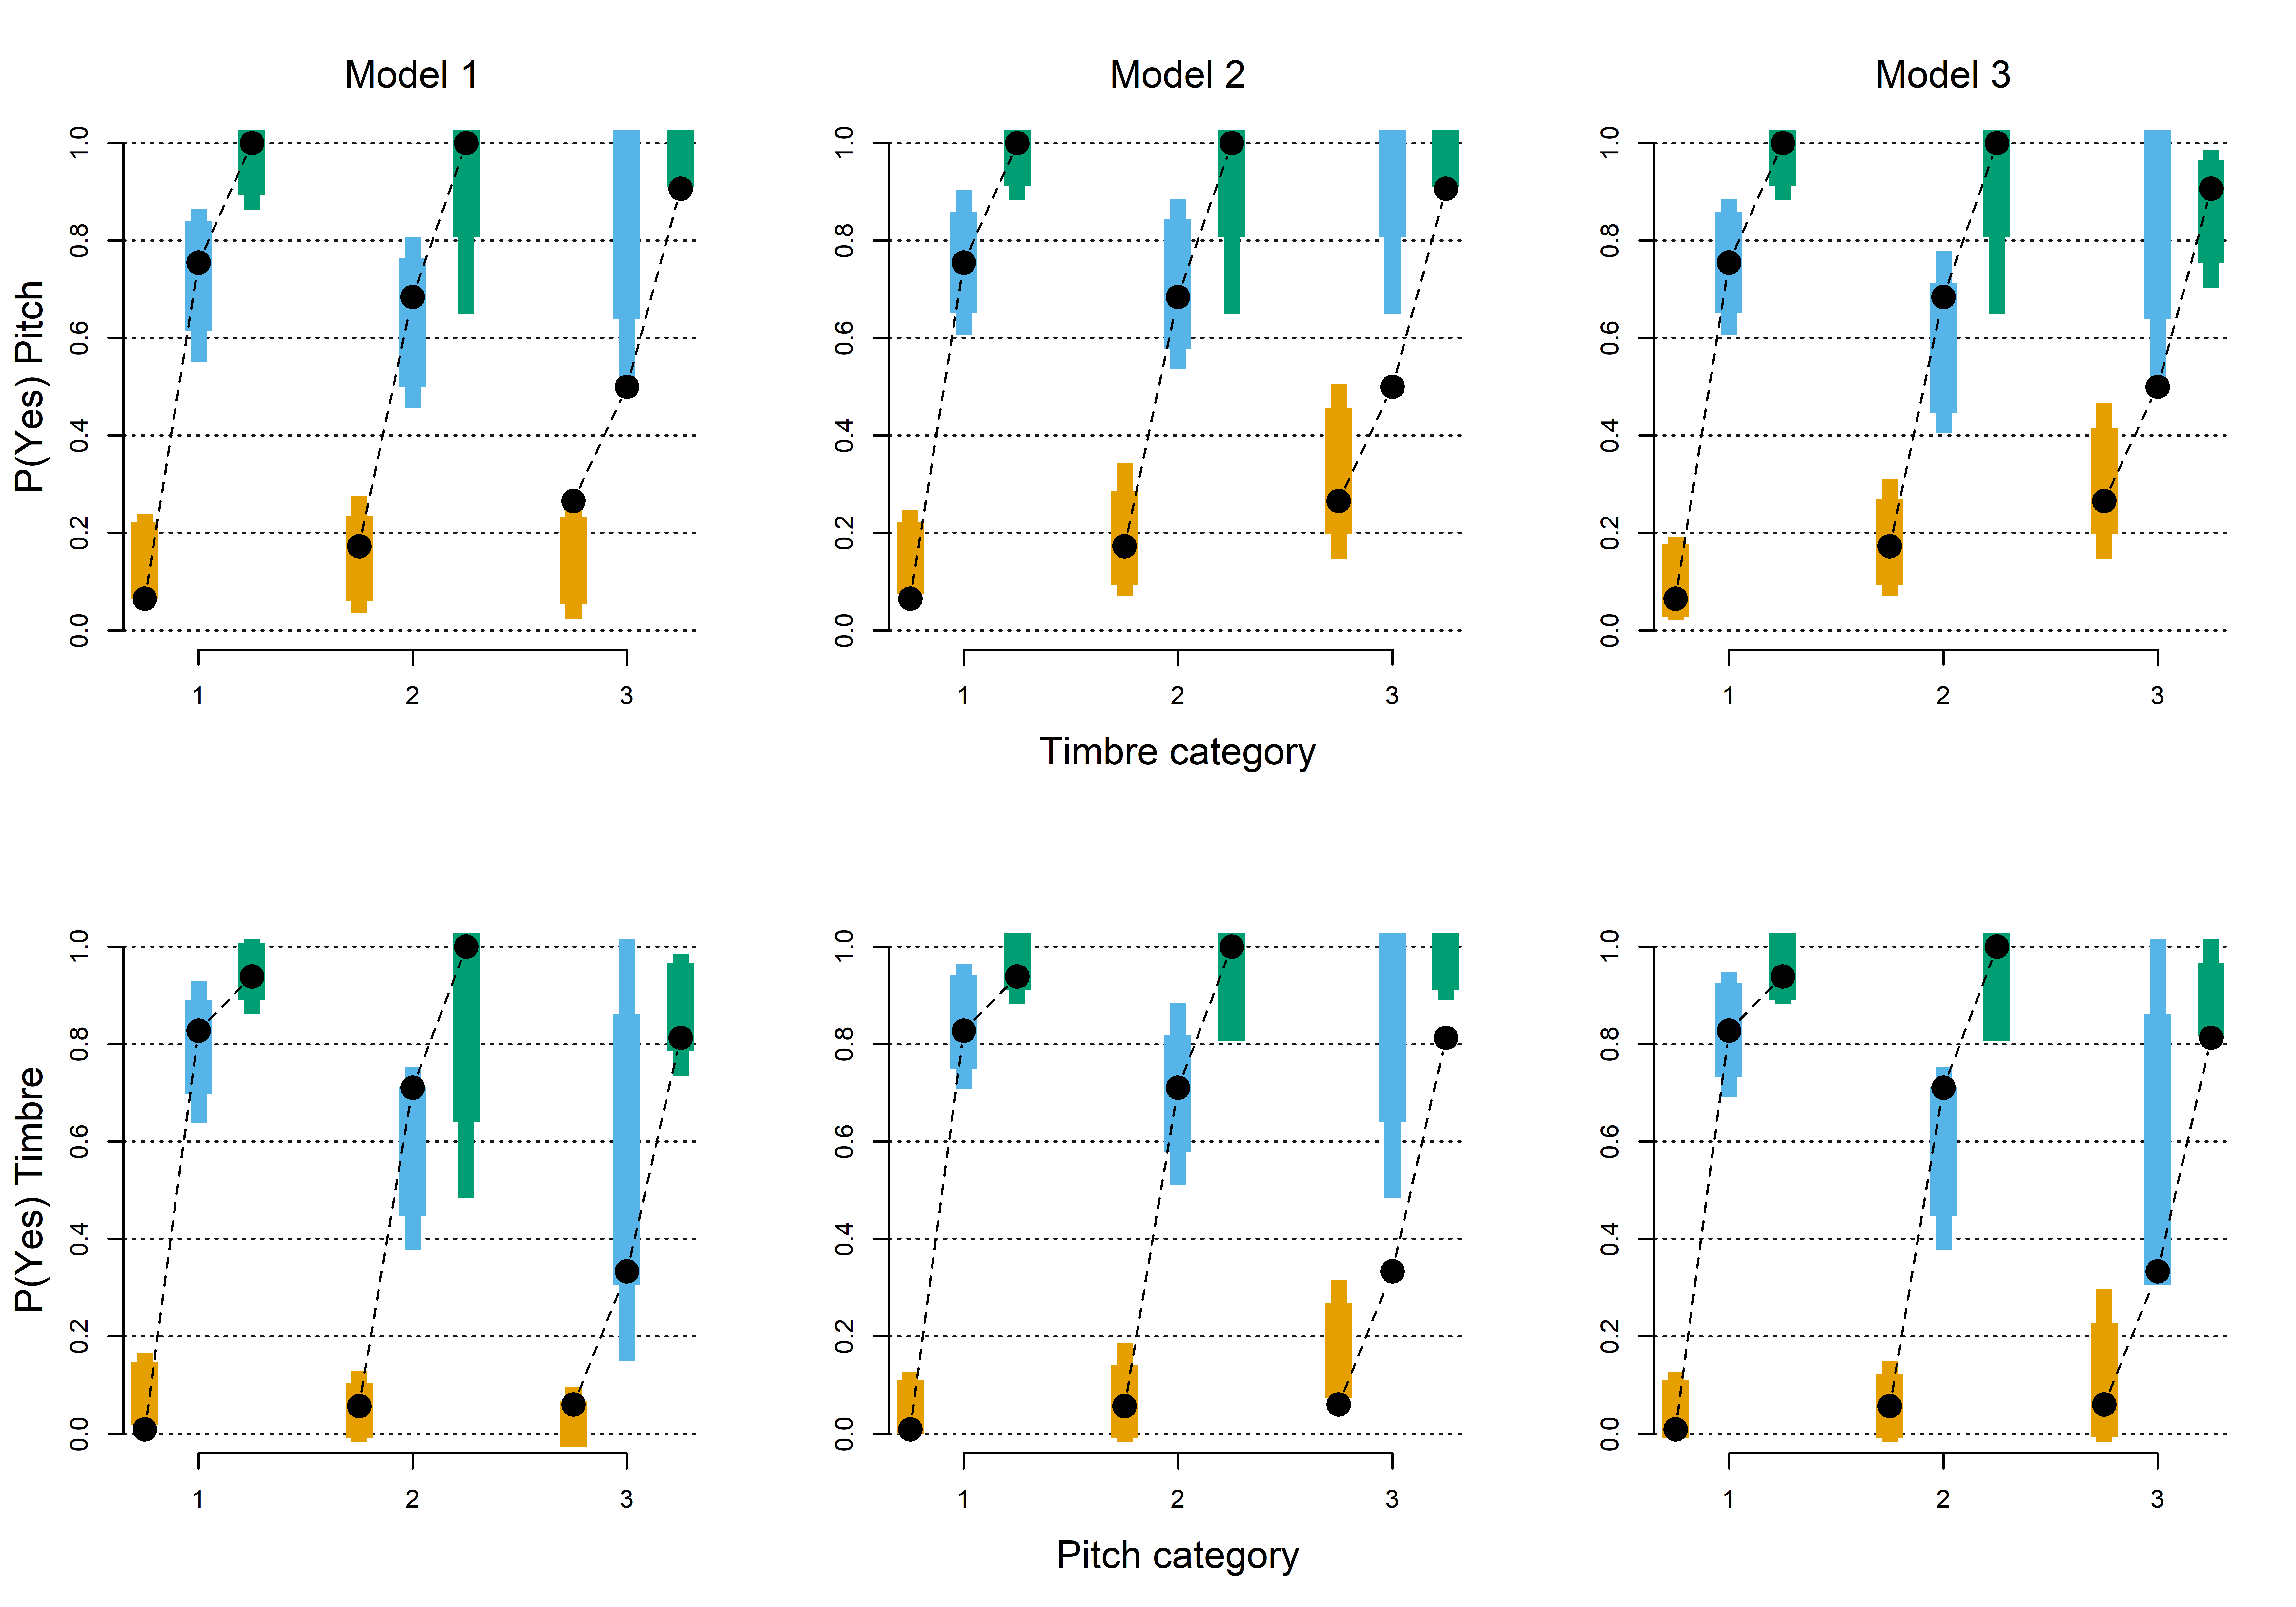
\includegraphics[scale=0.75, angle = 270]{Analysis_of_Human_Data/JP_YN_post_pred}
\caption{Task: Yes/No; Participant: JP. Posterior predictive distributions for parameters of Models 1 to 3.}
\label{fig:JP_YN_post_pred}
\end{figure}

\begin{figure}[H]
\centering
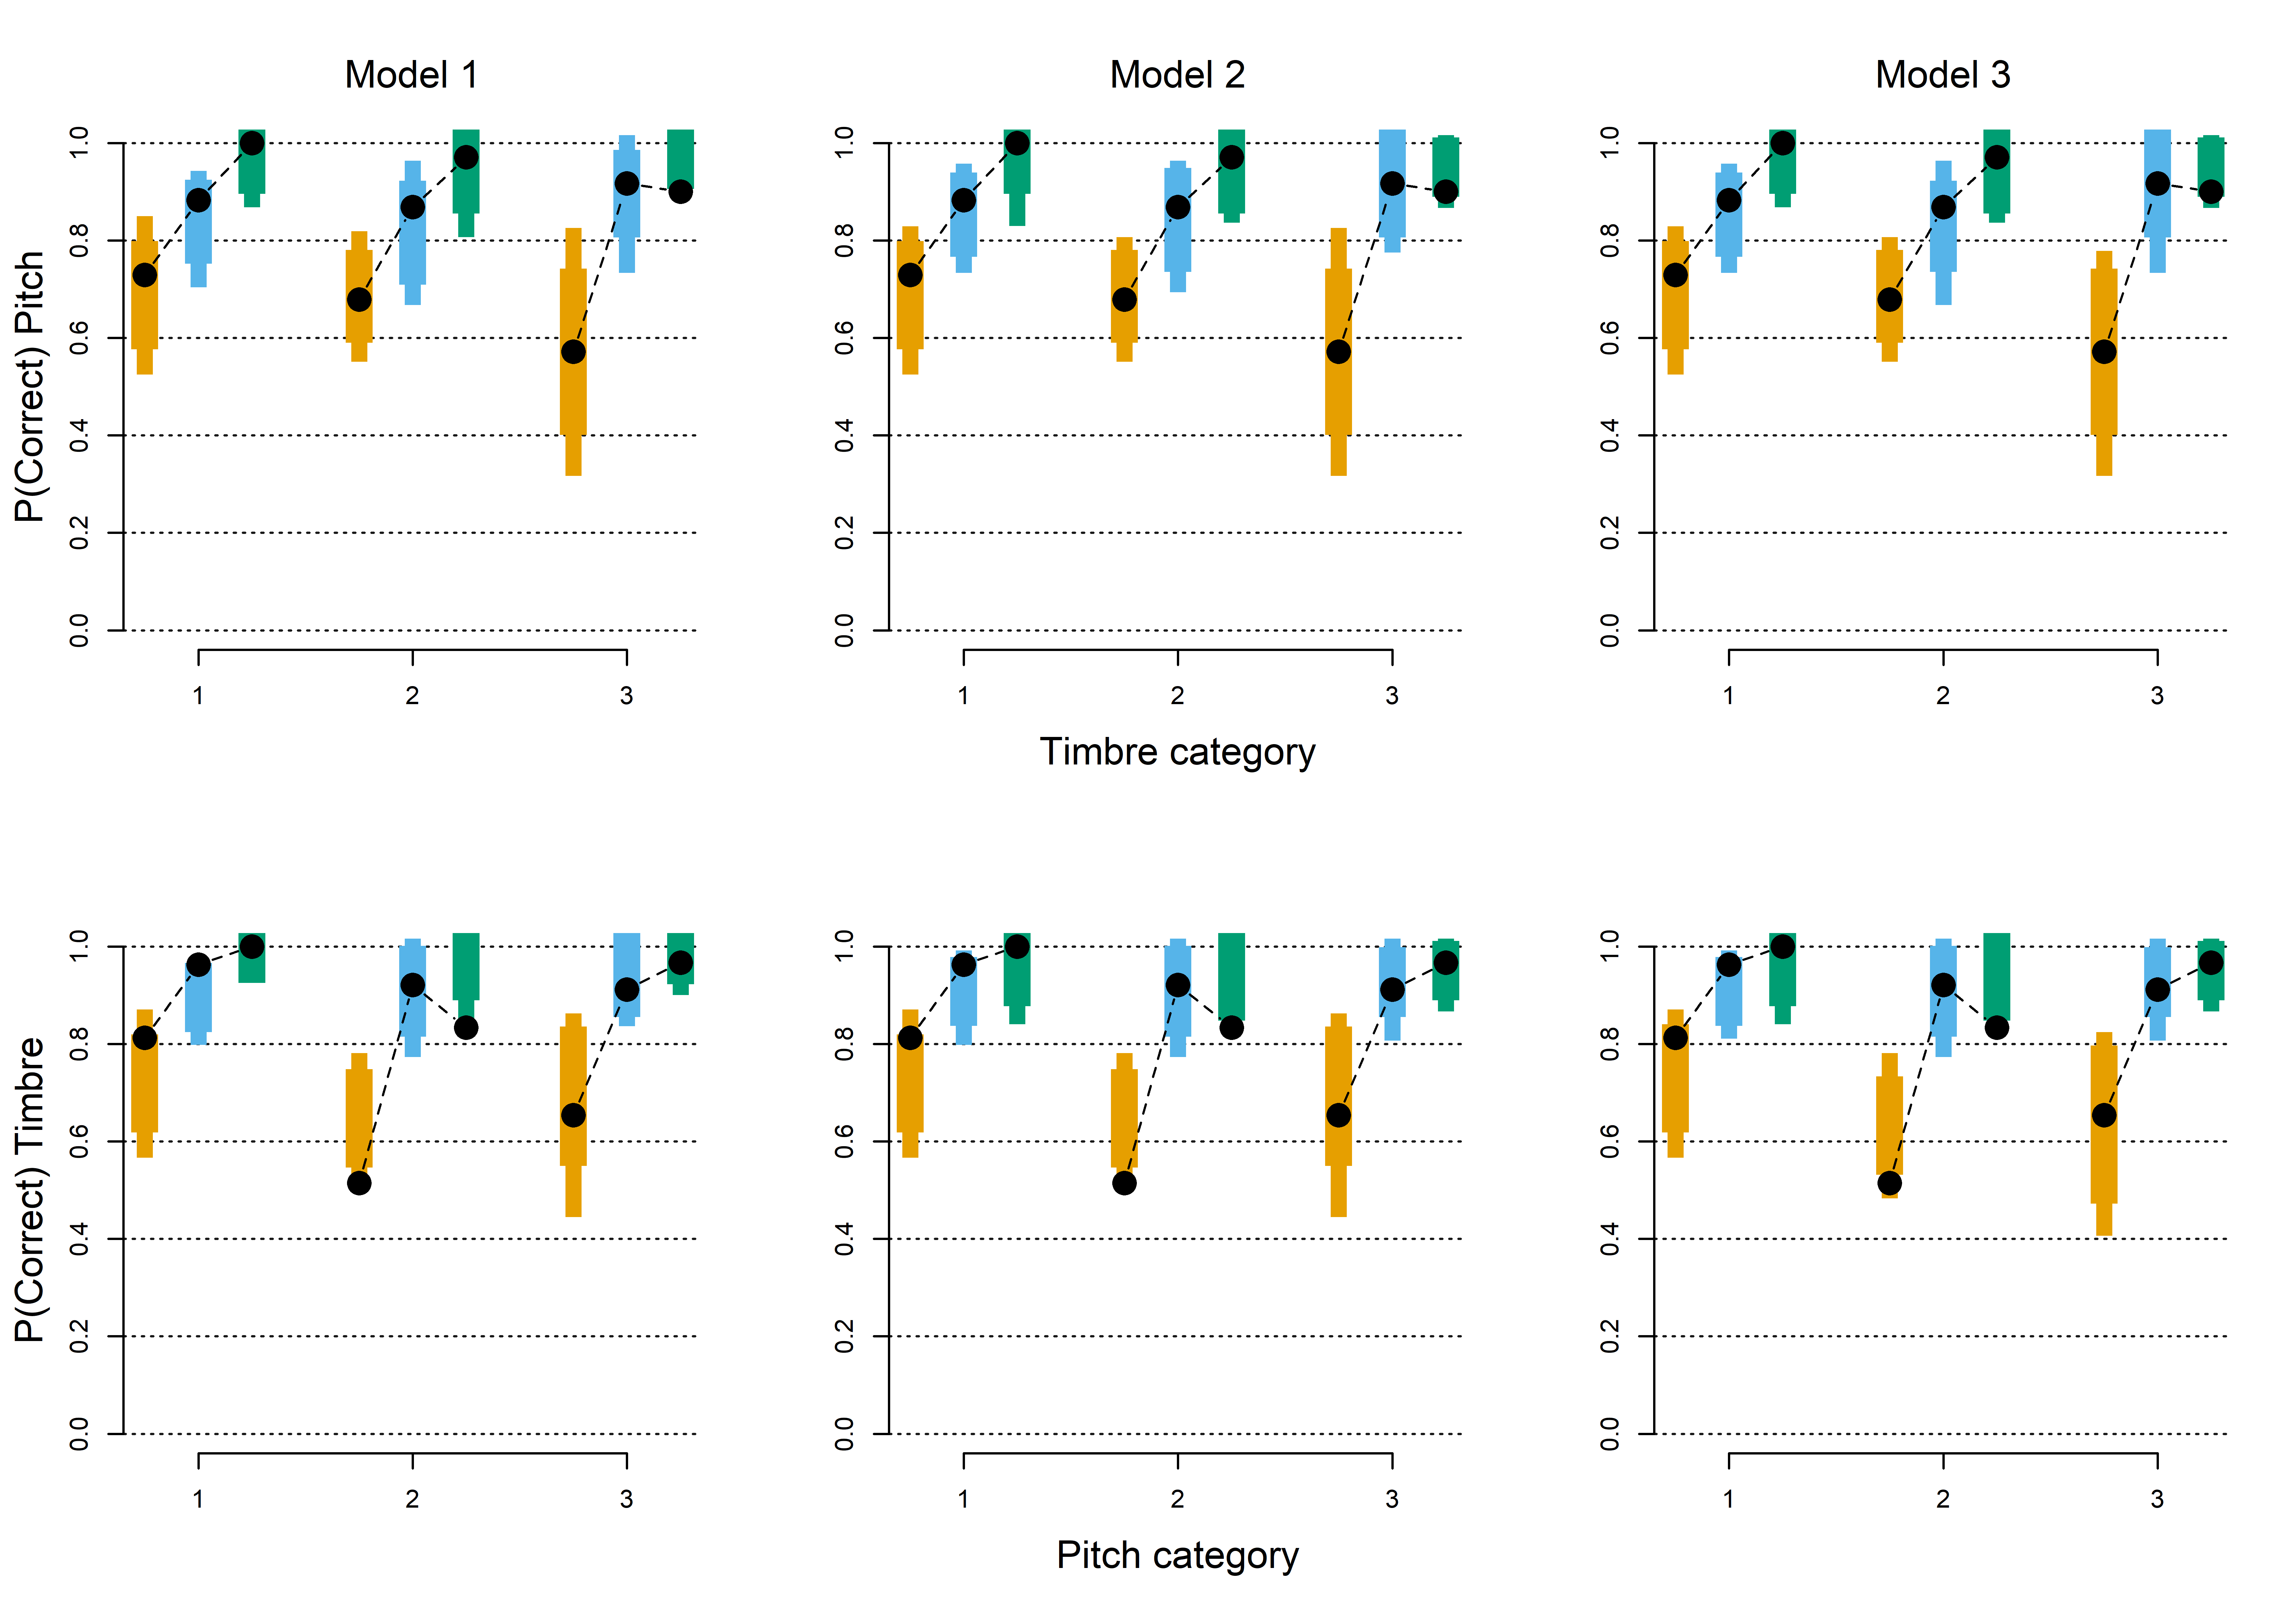
\includegraphics[scale=0.75, angle = 270]{Analysis_of_Human_Data/JP_AFC_post_pred}
\caption{Task: 2I-4AFC; Participant: JP. Posterior predictive distributions for parameters of Models 1 to 3.}
\label{fig:JP_AFC_post_pred}
\end{figure}

\paragraph{Participant JP, Models 1 to 3: Discussion}

Yes/No: In contrast to participant OK, here Model 3 (Figure \ref{fig:JP_YN_Basic_models}) seems to suffer from non-identifiabilities: sign for the $\kappa_{\sigma}$ parameter for \textit{timbre} dimension seems to not be identifiable from the data. The bimodality from the $\kappa_{\sigma}$ parameters seems to have bled to the criterion parameter on the \textit{timbre} dimension.

\subsubsection{Participant JP, Model with both interactions}

\begin{figure}[H]
\centering
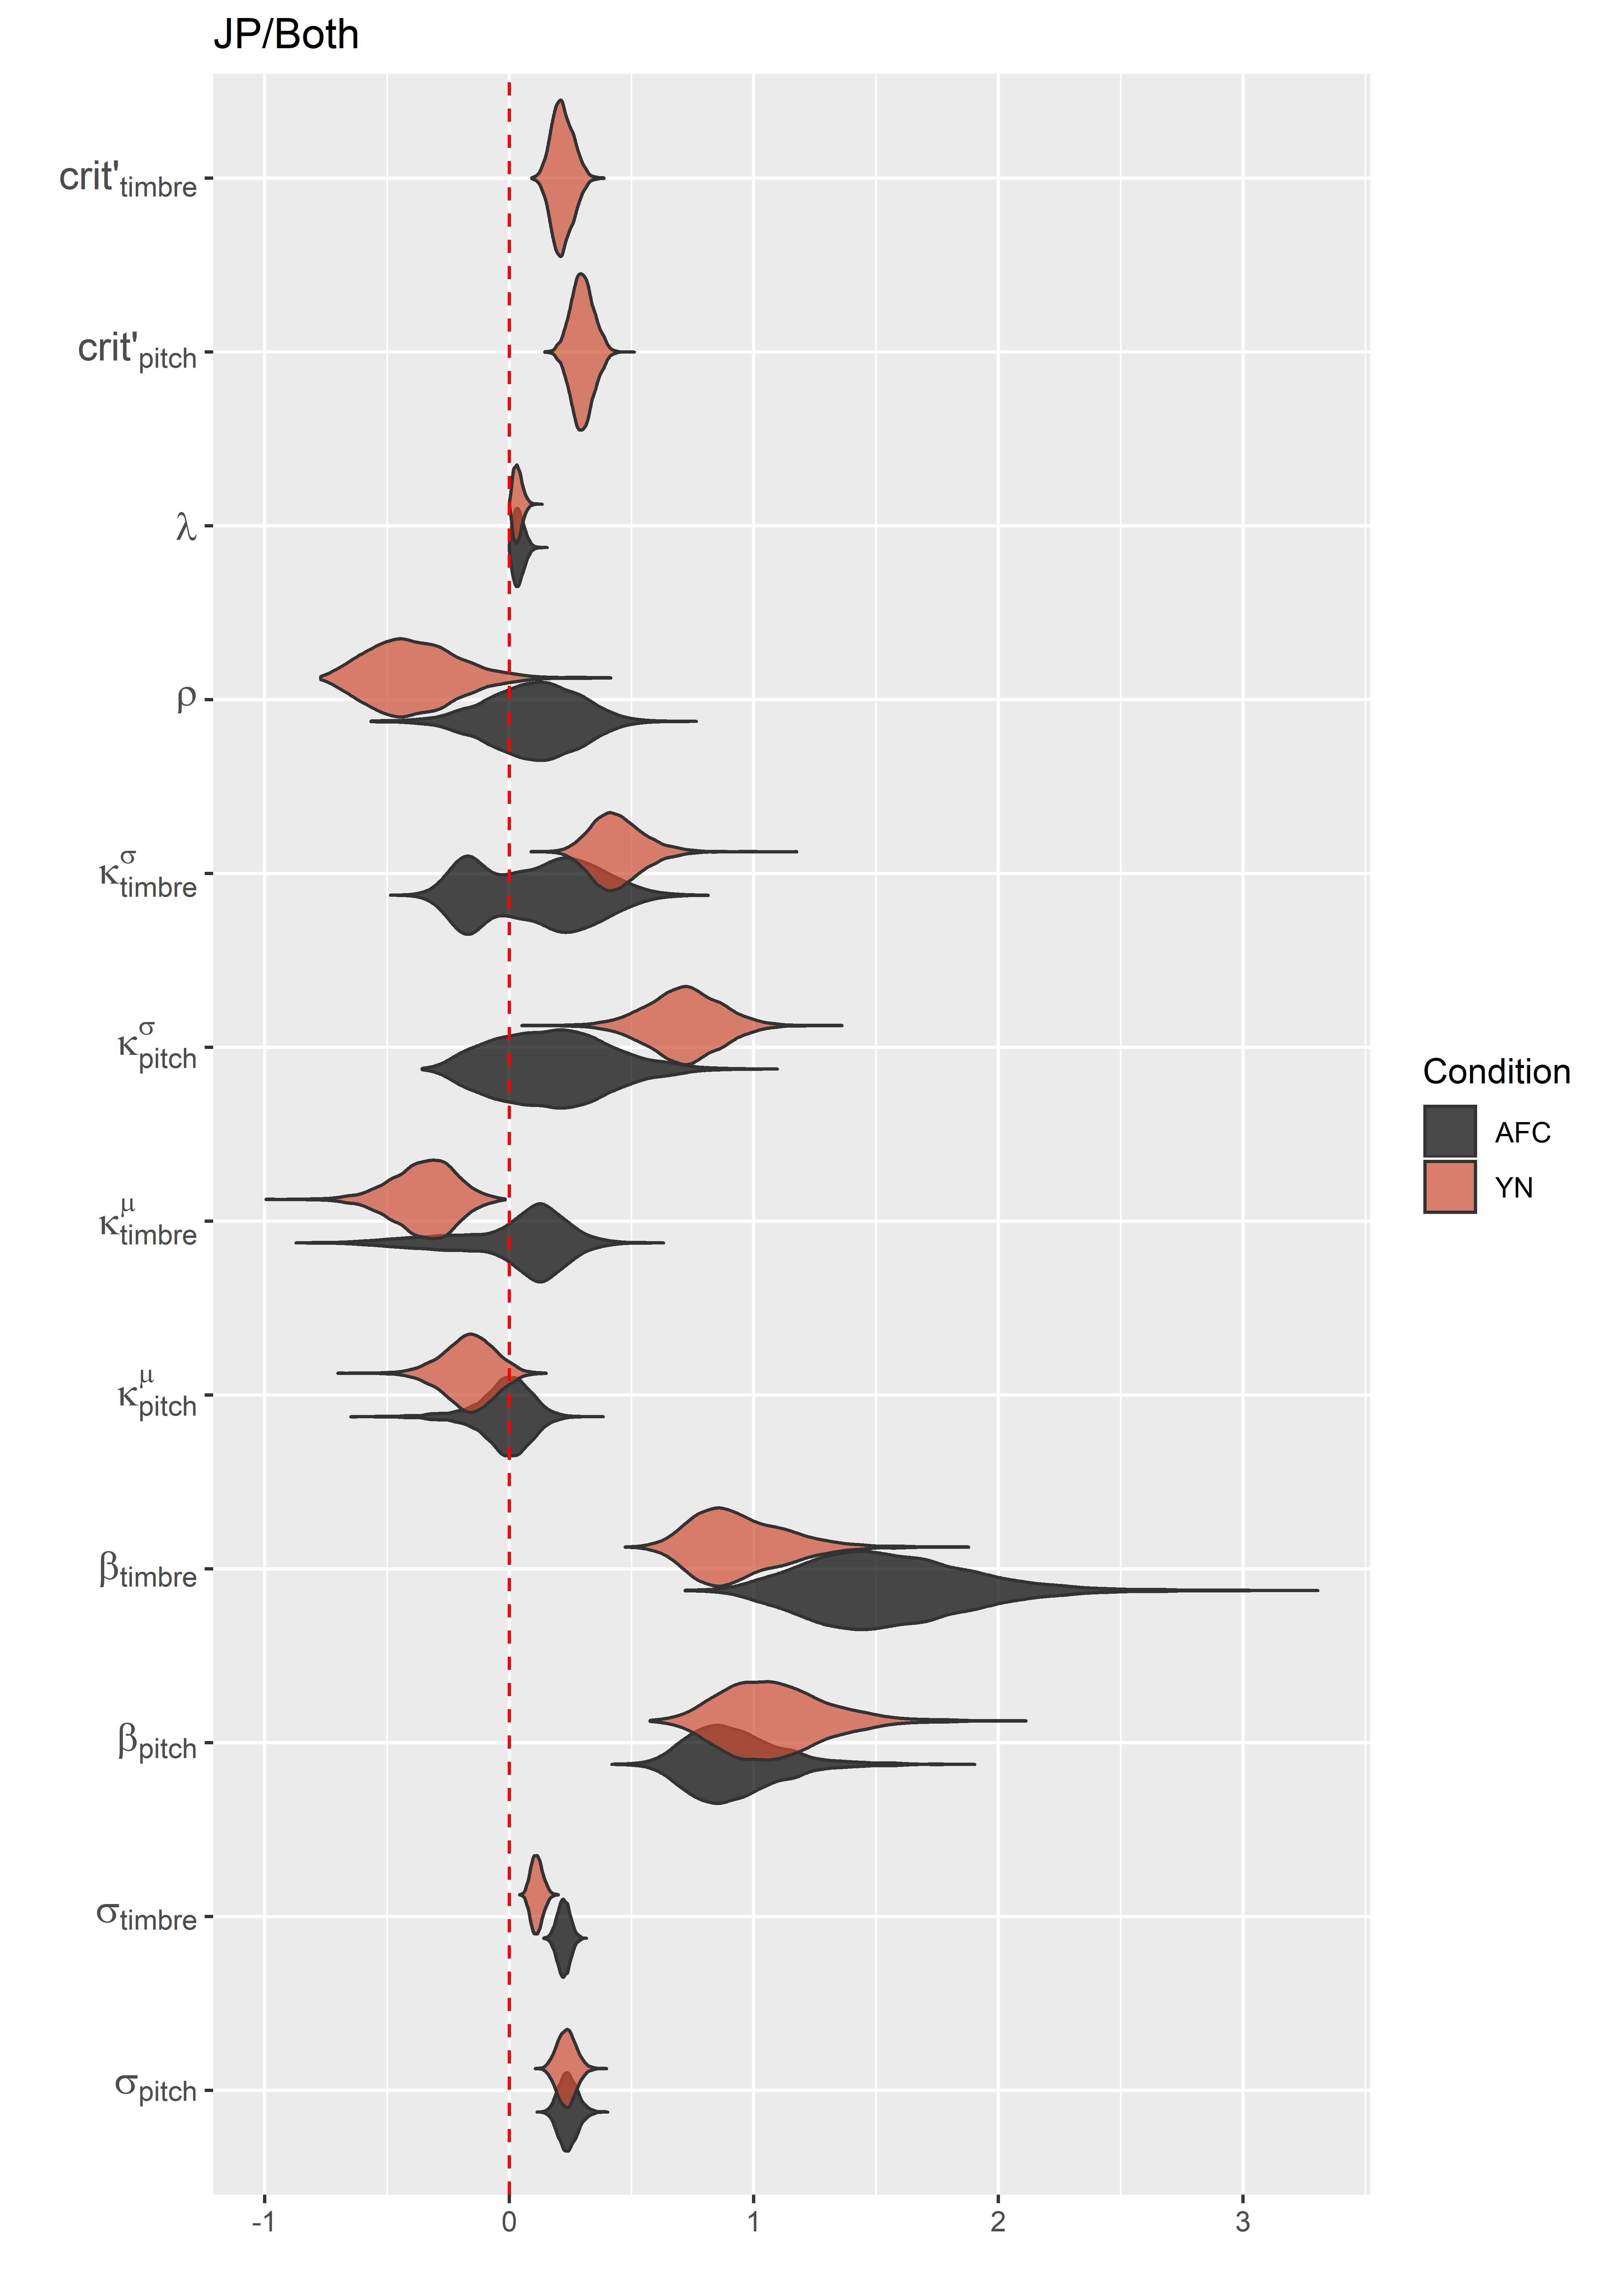
\includegraphics[scale=0.75, angle = 0]{Analysis_of_Human_Data/JP_YN_AFC_Both}
\caption{Both tasks; Participant: JP. Marginal posterior distributions for parameters of model with both interactions}
\label{fig:JP_YN_AFC_Both}
\end{figure}

\paragraph{Participant JP, Model with both interactions: Discussion}

As can be seen from the parameter estimates (Figure \ref{fig:JP_YN_AFC_Both}) the $\kappa_{\sigma}$ in the Yes/No task is not identifiable here either. To alleviate this problem, I constrained $\kappa_{sigma}$ to positive values. This seemed reasonable, since the parameter was identified as positive in the 2I-4AFC model, and on the grounds that pitch and timbre are usually thought to interfere negatively. 

\subsubsection{Participant JP, Model with both interactions, $\kappa_{\sigma} > 0$}

\begin{figure}[H]
\centering
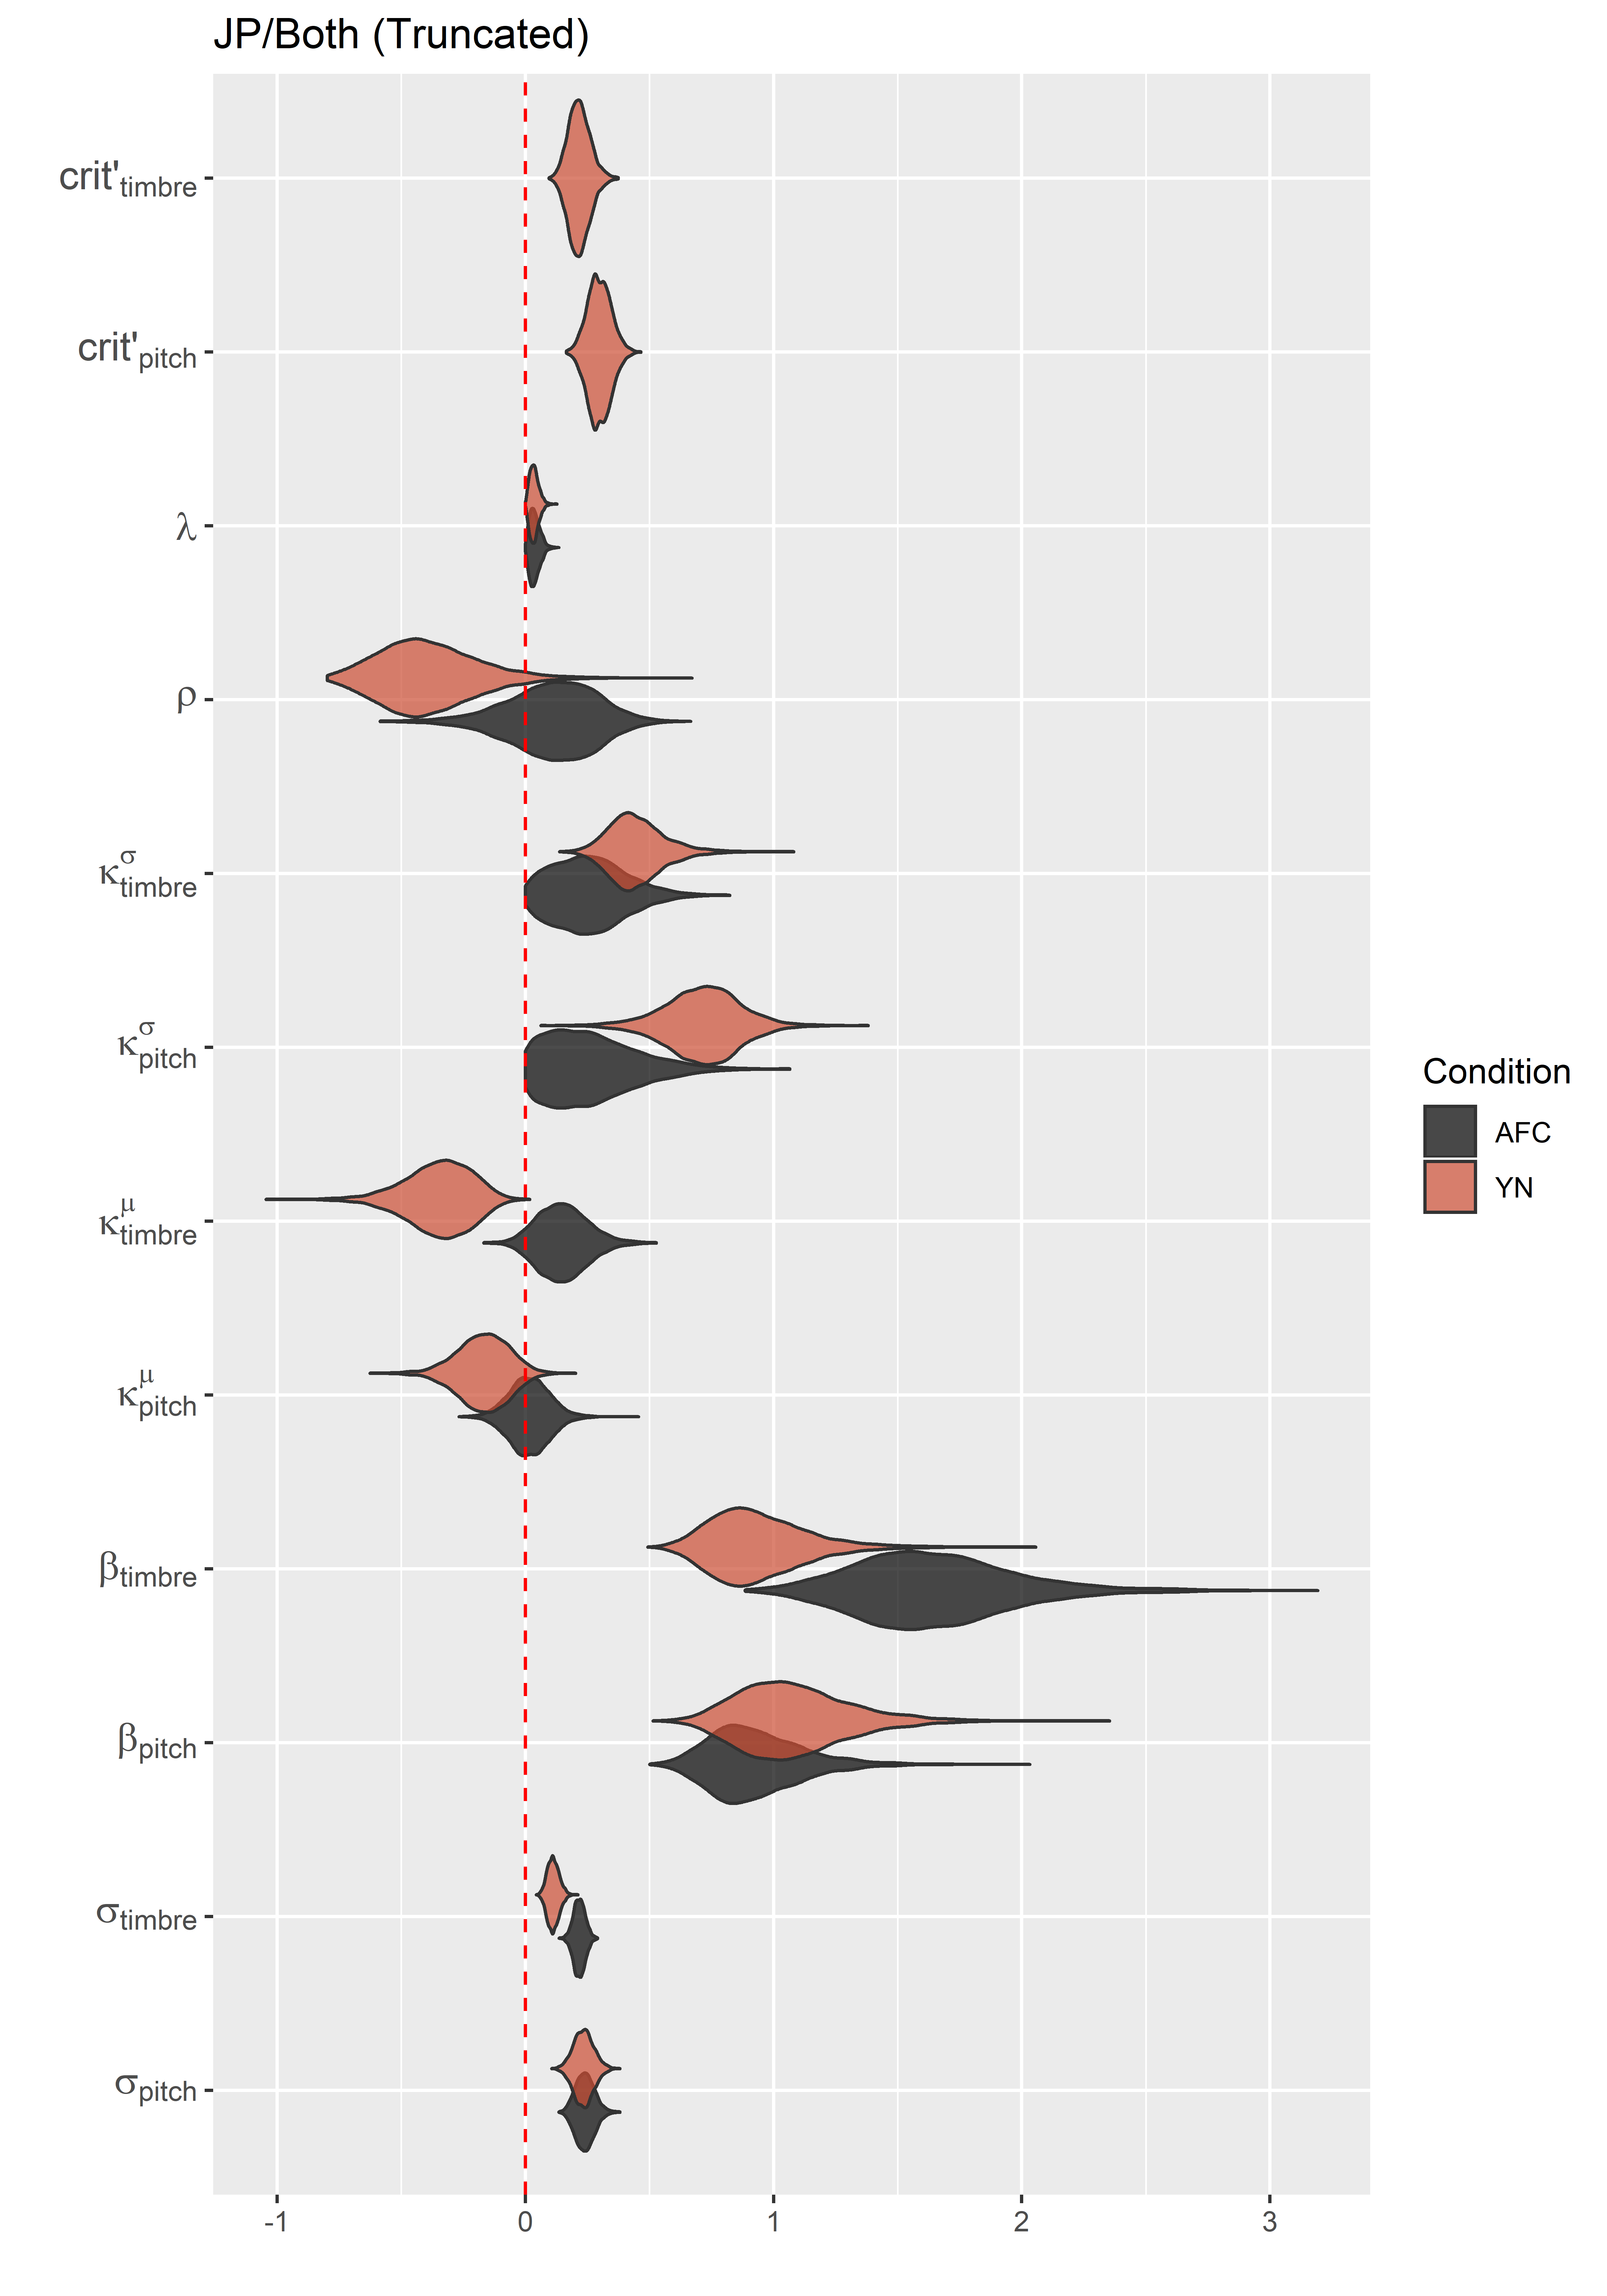
\includegraphics[scale=0.75, angle = 0]{Analysis_of_Human_Data/JP_YN_AFC_Both_T}
\caption{Both tasks; Participant: JP. Marginal posterior distributions for parameters of model with both interactions, and $\kappa_{\sigma} > 0$}
\label{fig:JP_YN_AFC_Both_T}
\end{figure}

\begin{figure}[H]
\centering
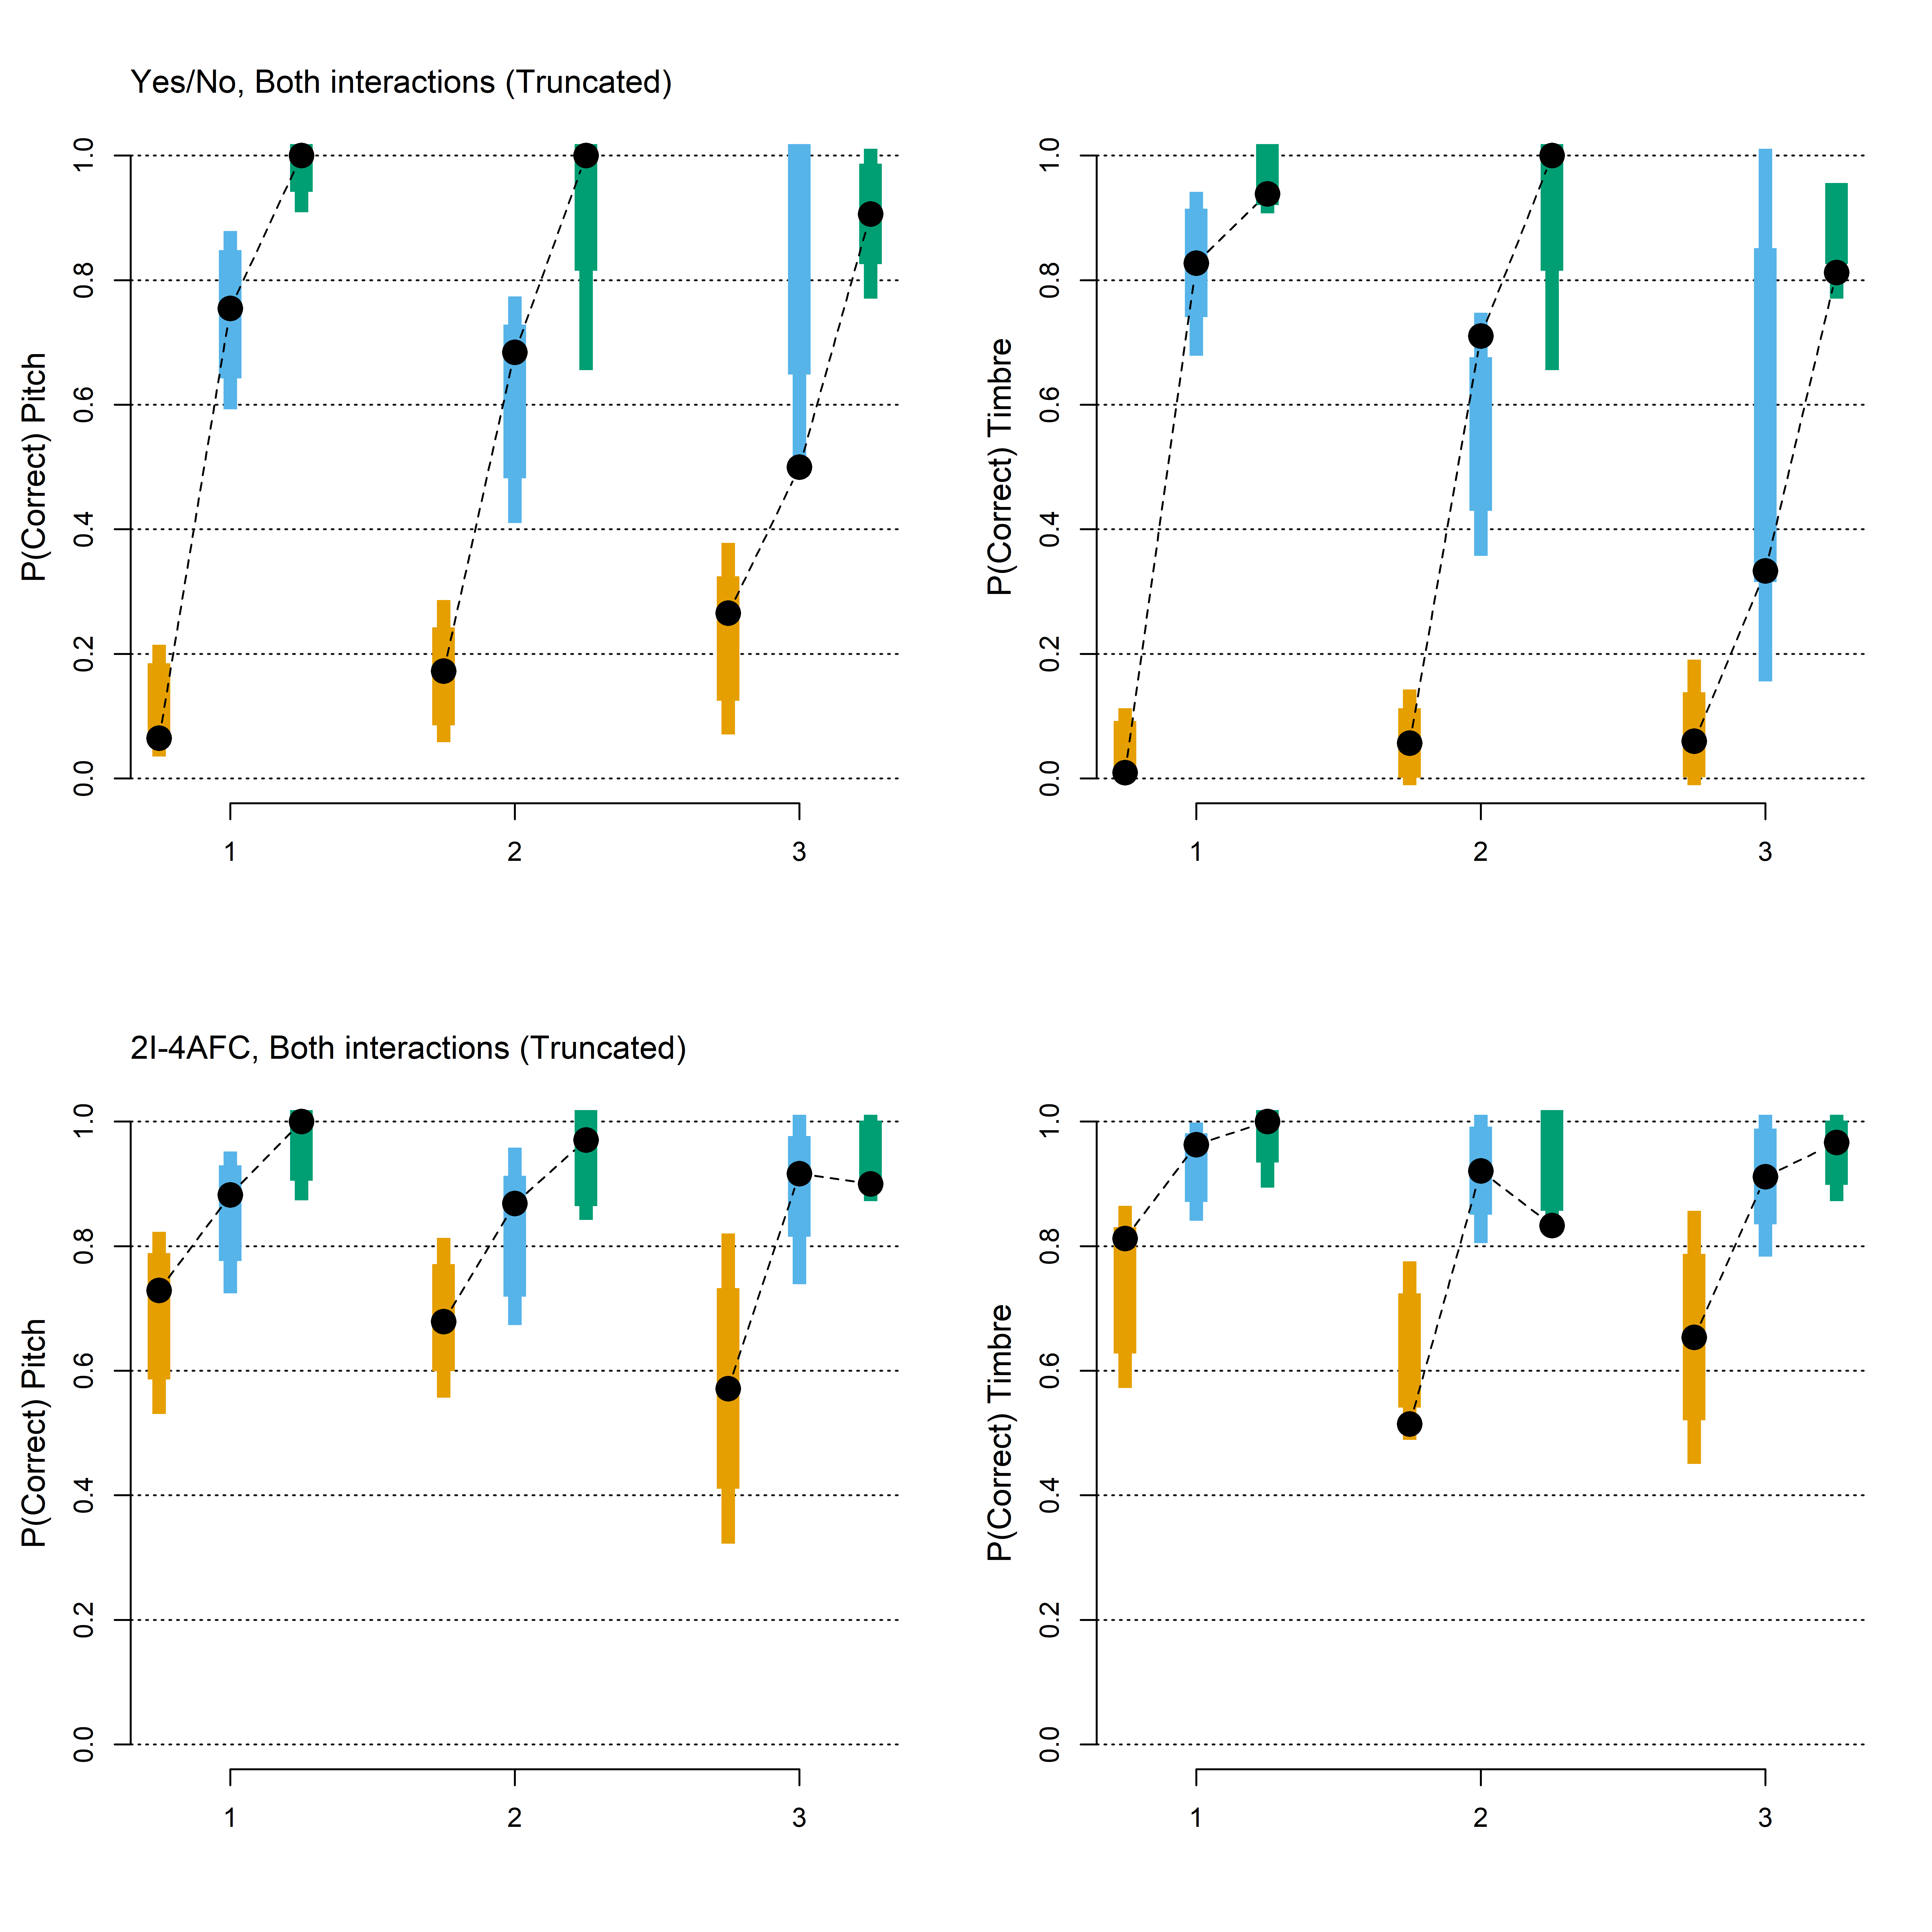
\includegraphics[scale=0.50, angle = 270]{Analysis_of_Human_Data/JP_post_pred_both_truncated}
\caption{Both tasks; Participant: JP. Marginal posterior distributions for parameters of model with both interactions, $\kappa_{\sigma} > 0$.}
\label{fig:JP_post_pred_both_truncated}
\end{figure}

\paragraph{Participant JP, Model with both interactions, $\kappa_{\sigma} > 0$: Discussion}

The posterior distributions don't exhibit obvious problems with the model (Figure \ref{fig:JP_YN_AFC_Both_T}) and the posterior predictive distribution (Figure \ref{fig:JP_post_pred_both_truncated}) indicates acceptable fit with the observed data.

\subsection{Some introspective remarks}
\label{sec:introspec}

While posterior predictive checking acts as a quantitative way to check (some) aspects of the models, I will be also incorporating more qualitative model critique in the form of introspective remarks. I've compiled and edited ones that I feel are most important regarding violations of the assumptions of the model in this section. 

I've chosen not to include the information about from which participant each remark is for three reasons: first, these are highly subjective and contingent on how each participant verbalizes their internal processes; second, some of the remarks can be conflicting, reflecting dynamic changes strategies or attention; and third, since there were only two participants, no inferences about the generalizability can be made anyway. However, these provide important information about the limitations of the models and tasks as implemented here; which ones are important and how they are to be remedied are questions left for future work. 

\begin{remark}
The response input style used for the 2I-AFC task here was difficult, and potentially lead to increased amount of lapses; at least it meant that the cognitive burden was greater in that task.
\end{remark}

\begin{remark}
In the 2I-4AFC task the overall sounds of the intervals were compared against each other more so than stimuli inside the intervals.
\end{remark}

\begin{remark}
Attention and decisional criteria were calibrated by immediately preceding stimuli. For example the internal idea of how stimulus in which there's change on both dimension sounds like was affected by preceding stimuli and responses to them. 
\end{remark}

\begin{remark}
Stimuli were attended sequentially: one of the dimensions was primary, and the decision whether it changed/in which interval it changed was made first. 
\end{remark}

\begin{remark}
In the 2I-4AFC task easily discriminable stimuli terminated attention to that dimension. E.g. if there was a clear change in timbre in the first interval, there was no need to listen to it on the second interval; instead, all attention could be diverted to listening for changes in pitch. 
\end{remark}

\begin{remark}
In the 2I-4AFC task if one of the dimensions was not discriminable and the other was, often the default choice was to pick the interval in which the more discriminable stimulus was, thinking that maybe the large stimulus masked the fainter.
\end{remark}

\begin{remark}
There was a lot of variability in how the response categories were used during the experiment.
\end{remark}

\subsection{General discussion}

\paragraph{Question 1: Was the original model (Model 1) sufficient?}

For participant OK Model 1 resulted in posterior distribution with two modes (Figure \ref{fig:OK_YN_Basic_models}), which is a clear sign of problems with the model. The marginal posterior distributions for participant JP are less problematic, but it is clear from the posterior predictive plots for both participants (Figures \ref{fig:OK_YN_post_pred} and \ref{fig:fig:JP_YN_post_pred}) that Model 1 fails to capture the fact that for both participants changes in the other dimension increase false alarm probability while decreasing the probability of a  hit. A pattern that is only explained by including the term $\kappa_{\sigma}$ to the model. 

For the 2I-4AFC models there aren't as great differences. 

The pattern of results in which the Yes/No model has more problems probably is due to that model being more diagnostic.    

\paragraph{Question 2: Did coefficients in the Yes/No and 2I-4AFC tasks correspond with each other?}

Due to problems with Models 1 to 3, I used models with both kinds of interactions (and with $\kappa_{\sigma} > 0$ for participant JP) to test the prediction that the coefficients from both tasks should be identical (when taking into account the reduced sensitivity in the 2I-4AFC task).

Results are summarized in Figures \ref{fig:OK_YN_AFC_Both} and \ref{fig:JP_YN_AFC_Both_T}. For both participants it seems that the sensory parameters ($\sigma$ and $\beta$) are fairly close to each other in both tasks. However, the interactions are more varied. 

Parameter $\kappa_{\mu}$ seems to be the most well-behaved  in this sense. For participant OK the $\kappa_{\mu}$ parameters suggest--strongly for the \textit{timbre} dimension--different signs for the coefficient; for participant JP these coefficients for the AFC model seem to lean towards zero, while for the YN model positive values are suggested. 

For both participants the $\rho$ parameters are drawn towards zero in the AFC model while strongly suggesting negative values in the YN model. 

\paragraph{Question 3: What inferences can we make about the processing of pitch and timbre?}

As already discussed, the interaction coefficients varied significantly across the two models, which suggest that the coefficients are strongly influenced by e.g. attention and decisional processes. This makes it hard to draw strong inferences.

Discussion will again be based on Figures \ref{fig:OK_YN_AFC_Both} and \ref{fig:JP_YN_AFC_Both_T}. For both participants the $\kappa_{\sigma}$ coefficients are positive for both \textit{pitch} and \textit{timbre}. This suggest that  changes on the other dimension increase the variability in the evidence distributions. 

For participant JP both $\kappa{\mu}$ coefficients are negative, suggesting that changes on the other dimension decrease the mean of the evidence on the other dimension, that is for example large timbral changes make pitch changes seem smaller (assuming that the evidence distribution reflects mainly perceptual processing).

In the AFC task $\kappa^{\mu}_\text{timbre}$ is mostly on the positive side, which would suggest that changes in pitch would make timbral changes seem larger; or that the participant becomes more prone to answering positively to \textit{timbre} dimension. 

\paragraph{Conclusions from introspection}

It is clear from the introspective remarks that many of the (implicit) assumptions of the models were violated. The remarks indicate for example non-stationarity, serial processing of the dimensions and autocorrelation between subsequent stimuli. Especially the 2I-4AFC task proved to be problematic due to the more complicated response scheme and complex stimuli.  To better diagnose these--and other--problems, more methods for posterior predictive checking should be developed, to increase the coverage of model criticism. 

\newpage

%!Rnw root = ../Joni_Paakko_-_Thesis.Rnw

\section{Conclusions}

The main theoretical contribution of this thesis is to add psychometric functions to GRT and define interactions through the coupling of these functions. Primary reason for this was to model response probabilities as a function of continuous stimulus values; the classic GRT models are used for categorial stimuli. This adds some structural assumptions to the model, such as, how to parameterize the relationship between physical signals and $d'$ values and how to couple the psychometric functions. The additional structural constraints help make more focused predictions, that--when they violate observed data--can be diagnostic of problems with the models, which in turn is important for model development. The classic categorical models suffer from over-fitting, which can mask such problems.

Another important difference (to classic GRT) is that instead of categorization I modelled discrimination. Since the perception of faint stimuli is more often based on the differences between stimuli, I believe models of (auditory) perception should take this into account, as it is a rather simple thing to do--although this does limit the selection of experimental tasks.  

As shown by  the simulations,  the adaptive method, unsurprisingly, was able to achieve better performance on average, however, the difference was rather small and was engulfed in a lot of variability. This suggests that adaptive sampling of stimuli offers little in terms of precision in parameter estimates. What I would believe to be sufficient would be to estimate psychometric functions for each dimension in the absence of interactions and adapt stimuli to these functions, separately for each dimension; similar to how adaptation was implemented for one-dimensional stimuli in \citet{kontsevichtyler1999}. 

There's a lot of variability in how well the generating parameters of the simulated observers are recovered. The $\kappa_{\mu}$ terms were recovered fairly fast, but the posterior distributions for $\rho$ parameters were left relatively wide. The central implication for future research is that it would be extremely difficult to for example try to infer the dependence of $\rho$ parameter on the stimulus values (which is sometimes done in classic GRT  models, see \citet{ashby2015, soto2017}), however for the $\kappa_{\mu}$ parameter this kind of inference seems more plausible.  
 
Data from the psychophysical experiments indicated rather poor fit of the initial model (the one that was used for the simulations), especially in the case of the observer OK. For this observer the data indicated that the main source of interaction between the dimensions was in how they influenced the standard deviations of the evidence distributions. For both observers I ended up using a model that included coefficients for both coupled means and standard deviations. 

The challenge that adaptive methods are facing when it comes to GRT related models is not necessarily how to minimize the entropy of the posterior distribution--as was done here--but rather how to make reliable inferences about the structural aspects of the models, and how to deal with e.g. the kind of non-identifiabilities that were discussed during the analysis of psychophysical data. For observer JP the sign of the parameter $\kappa_{\sigma}$ was not identifiable which required me to constrain the parameter to positive values. This suggests that strong prior information might be needed to identify the models completely--at least for some data sets.

The response input mechanism for the 2I-4AFC task proved to be problematic. I do believe that it is useful to compare parameter estimates from different tasks, since these provide  simple tests of  some predictions of the models, but the 2I-4AFC task, as it was implemented  here, was lacking. More intuitive methods for inputting responses should be developed. 

Despite these problems, the sensory parameters from the both tasks were fairly similar, suggesting some agreement with the theoretical predictions, however there were significant differences in the interaction parameters. This indicates strong influence from non-sensory sources. Identifying sensory and non-sensory sources of variability has been proven problematic even in SDT, as was discussed in Section \ref{sec:GRT} \textit{\nameref{sec:GRT}}, and it would seem, based on these data, that the problem might be even worse in GRT. 

\citet{garner1974} defined dimensional interactions as a set of \textit{converging operations}, that is from an array of different tasks, some of which required the participant to attend to both dimensions and some to just one (for a review see \citet{burns2014}). Indeed, this research by Garner greatly influenced the seminal paper on GRT (that is \citet{ashby1986}) in which one of the motivations was to unify these concepts under one theory. Since then, the task in which the participant is required to attend to both dimensions simultaneously has dominated the field, which was the case in this thesis.. Insights from the introspection point towards this assumption of simultaneous attention being problematic, and perhaps being one factor in why the interaction estimates from the two tasks diverged. For greater unification a model of what \textit{mode of attention} (that is, are they attending to the dimensions sequentially, is one of the primary, or are they attending to the wholes as a unity etc.) the participant is using in the task might be needed.

I made the assumption that the observer isn't significantly biased in the 2I-4AFC task. Due to the coding scheme (responses were coded as \textit{hits} and \textit{false alarms}), and not recording the actual intervals testing this assumption was not possible. The effects of bias on the parameter estimates should be explored more thoroughly.

\clearpage
\bibliography{references}
\bibliographystyle{apacite}

\newpage

%!Rnw root = ../Joni_Paakko_-_Thesis.Rnw

\appendix
\cftaddtitleline{toc}{section}{Appendices}{}

\section{Algorithm for calculating \texorpdfstring{$\phi_2$}{bivariate CDF}}

The algorithm is based on \citet{boys1989} and \citet{pan2017}.

\lstinputlisting{../Stan/bivariate_cdf.stan}

\newpage
\section{Code for models for the Yes/No task}

\subsection{Model 1}
\lstinputlisting{../Stan/mdlYN.stan}

\subsection{Model 2}
\lstinputlisting{../Stan/mdlYN_FL.stan}

\subsection{Model 3}
\lstinputlisting{../Stan/mdlYN_varshift_FL.stan}

\subsection{Both}
\lstinputlisting{../Stan/mdlYN_both.stan}

\subsection{Both (Truncated)}
\lstinputlisting{../Stan/mdlYN_both_truncated.stan}

\newpage
\section{Code for model for the 2I-4AFC task}

\subsection{Model 1}
\lstinputlisting{../Stan/mdlAFC.stan}

\subsection{Model 2}
\lstinputlisting{../Stan/mdlAFC_FL.stan}

\subsection{Model 3}
\lstinputlisting{../Stan/mdlAFC_varshift_FL.stan}

\subsection{Both}
\lstinputlisting{../Stan/mdlAFC_both.stan}


\end{document}
